\documentclass[twoside]{book}

% Packages required by doxygen
\usepackage{fixltx2e}
\usepackage{calc}
\usepackage{doxygen}
\usepackage[export]{adjustbox} % also loads graphicx
\usepackage{graphicx}
\usepackage[utf8]{inputenc}
\usepackage{makeidx}
\usepackage{multicol}
\usepackage{multirow}
\PassOptionsToPackage{warn}{textcomp}
\usepackage{textcomp}
\usepackage[nointegrals]{wasysym}
\usepackage[table]{xcolor}

% Font selection
\usepackage[T1]{fontenc}
\usepackage[scaled=.90]{helvet}
\usepackage{courier}
\usepackage{amssymb}
\usepackage{sectsty}
\renewcommand{\familydefault}{\sfdefault}
\allsectionsfont{%
  \fontseries{bc}\selectfont%
  \color{darkgray}%
}
\renewcommand{\DoxyLabelFont}{%
  \fontseries{bc}\selectfont%
  \color{darkgray}%
}
\newcommand{\+}{\discretionary{\mbox{\scriptsize$\hookleftarrow$}}{}{}}

% Page & text layout
\usepackage{geometry}
\geometry{%
  letterpaper,%
  top=2.5cm,%
  bottom=2.5cm,%
  left=2.5cm,%
  right=2.5cm%
}
\tolerance=750
\hfuzz=15pt
\hbadness=750
\setlength{\emergencystretch}{15pt}
\setlength{\parindent}{0cm}
\setlength{\parskip}{0.2cm}
\makeatletter
\renewcommand{\paragraph}{%
  \@startsection{paragraph}{4}{0ex}{-1.0ex}{1.0ex}{%
    \normalfont\normalsize\bfseries\SS@parafont%
  }%
}
\renewcommand{\subparagraph}{%
  \@startsection{subparagraph}{5}{0ex}{-1.0ex}{1.0ex}{%
    \normalfont\normalsize\bfseries\SS@subparafont%
  }%
}
\makeatother

% Headers & footers
\usepackage{fancyhdr}
\pagestyle{fancyplain}
\fancyhead[LE]{\fancyplain{}{\bfseries\thepage}}
\fancyhead[CE]{\fancyplain{}{}}
\fancyhead[RE]{\fancyplain{}{\bfseries\leftmark}}
\fancyhead[LO]{\fancyplain{}{\bfseries\rightmark}}
\fancyhead[CO]{\fancyplain{}{}}
\fancyhead[RO]{\fancyplain{}{\bfseries\thepage}}
\fancyfoot[LE]{\fancyplain{}{}}
\fancyfoot[CE]{\fancyplain{}{}}
\fancyfoot[RE]{\fancyplain{}{\bfseries\scriptsize Generated on Mon Jun 22 2015 12\+:44\+:59 for True\+North Time\+Warp Benchmark by Doxygen }}
\fancyfoot[LO]{\fancyplain{}{\bfseries\scriptsize Generated on Mon Jun 22 2015 12\+:44\+:59 for True\+North Time\+Warp Benchmark by Doxygen }}
\fancyfoot[CO]{\fancyplain{}{}}
\fancyfoot[RO]{\fancyplain{}{}}
\renewcommand{\footrulewidth}{0.4pt}
\renewcommand{\chaptermark}[1]{%
  \markboth{#1}{}%
}
\renewcommand{\sectionmark}[1]{%
  \markright{\thesection\ #1}%
}

% Indices & bibliography
\usepackage{natbib}
\usepackage[titles]{tocloft}
\setcounter{tocdepth}{3}
\setcounter{secnumdepth}{5}
\makeindex

% Hyperlinks (required, but should be loaded last)
\usepackage{ifpdf}
\ifpdf
  \usepackage[pdftex,pagebackref=true]{hyperref}
\else
  \usepackage[ps2pdf,pagebackref=true]{hyperref}
\fi
\hypersetup{%
  colorlinks=true,%
  linkcolor=blue,%
  citecolor=blue,%
  unicode%
}

% Custom commands
\newcommand{\clearemptydoublepage}{%
  \newpage{\pagestyle{empty}\cleardoublepage}%
}


%===== C O N T E N T S =====

\begin{document}

% Titlepage & ToC
\hypersetup{pageanchor=false,
             bookmarks=true,
             bookmarksnumbered=true,
             pdfencoding=unicode
            }
\pagenumbering{roman}
\begin{titlepage}
\vspace*{7cm}
\begin{center}%
{\Large True\+North Time\+Warp Benchmark }\\
\vspace*{1cm}
{\large Generated by Doxygen 1.8.9.1}\\
\vspace*{0.5cm}
{\small Mon Jun 22 2015 12:44:59}\\
\end{center}
\end{titlepage}
\clearemptydoublepage
\tableofcontents
\clearemptydoublepage
\pagenumbering{arabic}
\hypersetup{pageanchor=true}

%--- Begin generated contents ---
\chapter{Todo List}
\label{todo}
\hypertarget{todo}{}

\begin{DoxyRefList}
\item[\label{todo__todo000001}%
\hypertarget{todo__todo000001}{}%
global\+Scope$>$ Global \hyperlink{assist_8h_a4d378196b7fceed090d64ec8820b4065}{get\+Current\+Big\+Tick} (tw\+\_\+stime now)]\+: Implement \& determin if ε needs to be added to the return value. 
\item[\label{todo__todo000005}%
\hypertarget{todo__todo000005}{}%
global\+Scope$>$ Global \hyperlink{neuron_8h_a92d5882a15e11e2a6733483d51428e46}{neuron\+Should\+Fire} (\hyperlink{structneuron_state}{neuron\+State} $\ast$st)]check to see if this is needed, since it looks like just a simple if statement is in order. 
\item[\label{todo__todo000006}%
\hypertarget{todo__todo000006}{}%
Global \hyperlink{structneuron_state_a4199c14c5aabfd52f441e01623bdc84c}{neuron\+State\+:\+:dendrite\+Global\+Dest} ]\+: The dendrite\+Core and dendrite\+Local values might not be needed anymroe.  
\item[\label{todo__todo000002}%
\hypertarget{todo__todo000002}{}%
Module \hyperlink{neuron_8c_amgrpb71b6f136d39fa6c989fa9f8bce28fa9}{Reset\+Functions} ]\+: Check that reverse reset functions are needed, since previous voltage is stored in the neuron.  
\item[\label{todo__todo000003}%
\hypertarget{todo__todo000003}{}%
global\+Scope$>$ Global \hyperlink{neuron_8h_a2e78d7d2b70bf7349c3854b3727dcc25}{reset\+Linear} (void $\ast$neuron\+State)]\+: Check implementation against paper. 
\item[\label{todo__todo000004}%
\hypertarget{todo__todo000004}{}%
global\+Scope$>$ Global \hyperlink{neuron_8h_ae53276ccdb759ba1ea09806cbf9fc940}{reverse\+Reset\+Zero} (void $\ast$neuron\+State)]\+: Check that this is the proper way to handle reset zero function 
\end{DoxyRefList}
\chapter{Data Structure Index}
\section{Data Structures}
Here are the data structures with brief descriptions\+:\begin{DoxyCompactList}
\item\contentsline{section}{\hyperlink{structaxon_state}{axon\+State} }{\pageref{structaxon_state}}{}
\item\contentsline{section}{\hyperlink{structinput_simulator_state}{input\+Simulator\+State} \\*Struct that manages the spike generator }{\pageref{structinput_simulator_state}}{}
\item\contentsline{section}{\hyperlink{structleak_fun_del}{leak\+Fun\+Del} \\*This is a dec }{\pageref{structleak_fun_del}}{}
\item\contentsline{section}{\hyperlink{struct_msg___data}{Msg\+\_\+\+Data} \\*Main message struct }{\pageref{struct_msg___data}}{}
\item\contentsline{section}{\hyperlink{struct_neuron_model}{Neuron\+Model} \\*This struct maintains the state of an individual neuron.\+The neuron struct contains the parameters needed to maintain state in the neuron, along with references to output commands (dendrites) }{\pageref{struct_neuron_model}}{}
\item\contentsline{section}{\hyperlink{structneuron_state}{neuron\+State} }{\pageref{structneuron_state}}{}
\item\contentsline{section}{\hyperlink{structrandom_spikes}{random\+Spikes} \\*Struct that genreates spikes randomly }{\pageref{structrandom_spikes}}{}
\item\contentsline{section}{\hyperlink{unionreset_rate}{reset\+Rate} \\*Reset\+Rate This is a support union for neuron reset rates }{\pageref{unionreset_rate}}{}
\item\contentsline{section}{\hyperlink{structreverse_leak_del}{reverse\+Leak\+Del} \\*This fun }{\pageref{structreverse_leak_del}}{}
\item\contentsline{section}{\hyperlink{structselected_spikes}{selected\+Spikes} }{\pageref{structselected_spikes}}{}
\item\contentsline{section}{\hyperlink{structsynapse_state}{synapse\+State} \\*Synapse state structure }{\pageref{structsynapse_state}}{}
\end{DoxyCompactList}

\chapter{File Index}
\section{File List}
Here is a list of all files with brief descriptions\+:\begin{DoxyCompactList}
\item\contentsline{section}{/\+Users/\+Mark/\+Development/\+True\+North/tnt\+\_\+benchmark/\hyperlink{assist_8c}{assist.\+c} }{\pageref{assist_8c}}{}
\item\contentsline{section}{/\+Users/\+Mark/\+Development/\+True\+North/tnt\+\_\+benchmark/\hyperlink{assist_8h}{assist.\+h} }{\pageref{assist_8h}}{}
\item\contentsline{section}{/\+Users/\+Mark/\+Development/\+True\+North/tnt\+\_\+benchmark/\hyperlink{mappings_8c}{mappings.\+c} }{\pageref{mappings_8c}}{}
\item\contentsline{section}{/\+Users/\+Mark/\+Development/\+True\+North/tnt\+\_\+benchmark/\hyperlink{model__main_8c}{model\+\_\+main.\+c} }{\pageref{model__main_8c}}{}
\item\contentsline{section}{/\+Users/\+Mark/\+Development/\+True\+North/tnt\+\_\+benchmark/\hyperlink{model__main_8h}{model\+\_\+main.\+h} }{\pageref{model__main_8h}}{}
\item\contentsline{section}{/\+Users/\+Mark/\+Development/\+True\+North/tnt\+\_\+benchmark/\hyperlink{spike__generator_8c}{spike\+\_\+generator.\+c} }{\pageref{spike__generator_8c}}{}
\item\contentsline{section}{/\+Users/\+Mark/\+Development/\+True\+North/tnt\+\_\+benchmark/\hyperlink{spike__generator_8h}{spike\+\_\+generator.\+h} \\*Spike\+\_\+generate defines a L\+P state and functions that generate output at a tuneable rate }{\pageref{spike__generator_8h}}{}
\item\contentsline{section}{\hyperlink{mapping__specifications_8rtf}{mapping\+\_\+specifications.\+rtf} }{\pageref{mapping__specifications_8rtf}}{}
\item\contentsline{section}{/\+Users/\+Mark/\+Development/\+True\+North/tnt\+\_\+benchmark/models/\hyperlink{neuron__model_8c}{neuron\+\_\+model.\+c} }{\pageref{neuron__model_8c}}{}
\item\contentsline{section}{/\+Users/\+Mark/\+Development/\+True\+North/tnt\+\_\+benchmark/models/\hyperlink{neuron__model_8h}{neuron\+\_\+model.\+h} }{\pageref{neuron__model_8h}}{}
\item\contentsline{section}{/\+Users/\+Mark/\+Development/\+True\+North/tnt\+\_\+benchmark/models/\hyperlink{synapse_8h}{synapse.\+h} }{\pageref{synapse_8h}}{}
\end{DoxyCompactList}

\chapter{Data Structure Documentation}
\hypertarget{structaxon_state}{}\section{axon\+State Struct Reference}
\label{structaxon_state}\index{axon\+State@{axon\+State}}


{\ttfamily \#include $<$axon.\+h$>$}

\subsection*{Data Fields}
\begin{DoxyCompactItemize}
\item 
\hyperlink{assist_8h_ad77e6fc5a9b03d46e7c97b7c4b92e89f}{\+\_\+stat\+T} \hyperlink{structaxon_state_a7fc444364b1559859bccdf91f1e95475}{recv\+Msg\+Count}
\item 
\hyperlink{assist_8h_ad77e6fc5a9b03d46e7c97b7c4b92e89f}{\+\_\+stat\+T} \hyperlink{structaxon_state_a217ba44fb923dc4dc62bb73b14e61517}{send\+Msg\+Count}
\item 
tw\+\_\+lpid \hyperlink{structaxon_state_a665999819b255f36d756f17b85bc9a03}{dest\+Synapse}
\end{DoxyCompactItemize}


\subsection{Detailed Description}


Definition at line \hyperlink{axon_8h_source_l00014}{14} of file \hyperlink{axon_8h_source}{axon.\+h}.



\subsection{Field Documentation}
\hypertarget{structaxon_state_a665999819b255f36d756f17b85bc9a03}{}\index{axon\+State@{axon\+State}!dest\+Synapse@{dest\+Synapse}}
\index{dest\+Synapse@{dest\+Synapse}!axon\+State@{axon\+State}}
\subsubsection[{dest\+Synapse}]{\setlength{\rightskip}{0pt plus 5cm}tw\+\_\+lpid dest\+Synapse}\label{structaxon_state_a665999819b255f36d756f17b85bc9a03}


Definition at line \hyperlink{axon_8h_source_l00017}{17} of file \hyperlink{axon_8h_source}{axon.\+h}.

\hypertarget{structaxon_state_a7fc444364b1559859bccdf91f1e95475}{}\index{axon\+State@{axon\+State}!recv\+Msg\+Count@{recv\+Msg\+Count}}
\index{recv\+Msg\+Count@{recv\+Msg\+Count}!axon\+State@{axon\+State}}
\subsubsection[{recv\+Msg\+Count}]{\setlength{\rightskip}{0pt plus 5cm}{\bf \+\_\+stat\+T} recv\+Msg\+Count}\label{structaxon_state_a7fc444364b1559859bccdf91f1e95475}


Definition at line \hyperlink{axon_8h_source_l00015}{15} of file \hyperlink{axon_8h_source}{axon.\+h}.

\hypertarget{structaxon_state_a217ba44fb923dc4dc62bb73b14e61517}{}\index{axon\+State@{axon\+State}!send\+Msg\+Count@{send\+Msg\+Count}}
\index{send\+Msg\+Count@{send\+Msg\+Count}!axon\+State@{axon\+State}}
\subsubsection[{send\+Msg\+Count}]{\setlength{\rightskip}{0pt plus 5cm}{\bf \+\_\+stat\+T} send\+Msg\+Count}\label{structaxon_state_a217ba44fb923dc4dc62bb73b14e61517}


Definition at line \hyperlink{axon_8h_source_l00016}{16} of file \hyperlink{axon_8h_source}{axon.\+h}.



The documentation for this struct was generated from the following file\+:\begin{DoxyCompactItemize}
\item 
/\+Users/\+Mark/\+Development/\+True\+North/tnt\+\_\+benchmark/models/\hyperlink{axon_8h}{axon.\+h}\end{DoxyCompactItemize}

\hypertarget{structinput_simulator_state}{}\section{input\+Simulator\+State Struct Reference}
\label{structinput_simulator_state}\index{input\+Simulator\+State@{input\+Simulator\+State}}


Struct that manages the spike generator.  




{\ttfamily \#include $<$input\+\_\+simulator.\+h$>$}

\subsection*{Data Fields}
\begin{DoxyCompactItemize}
\item 
int \hyperlink{structinput_simulator_state_af892db49cef1c5e5d95010561e549678}{outbound}
\begin{DoxyCompactList}\small\item\em Represents how many conenctions the input system is attached to in spike\+\_\+generator\+\_\+model\+::outbound. \end{DoxyCompactList}\item 
tw\+\_\+lpid $\ast$ \hyperlink{structinput_simulator_state_a569dc67b8984bb0a3616bf17f9763ebb}{connected\+Synapses}
\begin{DoxyCompactList}\small\item\em An array of synapses that this is Random\+Spikes is attached to. \end{DoxyCompactList}\item 
\hyperlink{input__simulator_8h_aa47e87d309aab7727810011578bae86e}{spike\+Gen\+Del} \hyperlink{structinput_simulator_state_ae40f21a48f3157bcad074f424046ed2c}{spike\+Gen}
\item 
int $\ast$ \hyperlink{structinput_simulator_state_a666eb9ad96121cf3e4ce134e1a4c12c0}{output\+Mesh}
\begin{DoxyCompactList}\small\item\em Array that represents the output levels per tick. \end{DoxyCompactList}\item 
int \hyperlink{structinput_simulator_state_a97727a3be0dbd5813f860c99733048a8}{output\+Mesh\+Lengh}
\begin{DoxyCompactList}\small\item\em Size of the output mesh. \end{DoxyCompactList}\item 
float \hyperlink{structinput_simulator_state_a1333eb5695ae83d1ffccf24b08bc6288}{random\+Rate}
\begin{DoxyCompactList}\small\item\em If the random value is over this, spike. \end{DoxyCompactList}\item 
\hyperlink{input__simulator_8h_aa0d25534cd73156287b1136dd89c0215}{selected\+Random} \hyperlink{structinput_simulator_state_a18766f12fc4212349fb61b221f83b779}{rand\+Method}
\begin{DoxyCompactList}\small\item\em Selected random generator. \end{DoxyCompactList}\item 
float \hyperlink{structinput_simulator_state_a0eb8199754a403ccc8eac256f9193a02}{rnd\+Fct\+Val}
\begin{DoxyCompactList}\small\item\em For functions that need a second parameter (eg, binomial etc.), this is the second parameter. \end{DoxyCompactList}\item 
int \hyperlink{structinput_simulator_state_accc0c3f890194cda401a16f5f54e43cb}{current\+Out}
\begin{DoxyCompactList}\small\item\em current\+Out is the currently selected output synapse. \end{DoxyCompactList}\end{DoxyCompactItemize}


\subsection{Detailed Description}
Struct that manages the spike generator. 

Generally, there should be one of these per simulation! 

Definition at line \hyperlink{input__simulator_8h_source_l00042}{42} of file \hyperlink{input__simulator_8h_source}{input\+\_\+simulator.\+h}.



\subsection{Field Documentation}
\hypertarget{structinput_simulator_state_a569dc67b8984bb0a3616bf17f9763ebb}{}\index{input\+Simulator\+State@{input\+Simulator\+State}!connected\+Synapses@{connected\+Synapses}}
\index{connected\+Synapses@{connected\+Synapses}!input\+Simulator\+State@{input\+Simulator\+State}}
\subsubsection[{connected\+Synapses}]{\setlength{\rightskip}{0pt plus 5cm}tw\+\_\+lpid$\ast$ connected\+Synapses}\label{structinput_simulator_state_a569dc67b8984bb0a3616bf17f9763ebb}


An array of synapses that this is Random\+Spikes is attached to. 



Definition at line \hyperlink{input__simulator_8h_source_l00044}{44} of file \hyperlink{input__simulator_8h_source}{input\+\_\+simulator.\+h}.

\hypertarget{structinput_simulator_state_accc0c3f890194cda401a16f5f54e43cb}{}\index{input\+Simulator\+State@{input\+Simulator\+State}!current\+Out@{current\+Out}}
\index{current\+Out@{current\+Out}!input\+Simulator\+State@{input\+Simulator\+State}}
\subsubsection[{current\+Out}]{\setlength{\rightskip}{0pt plus 5cm}int current\+Out}\label{structinput_simulator_state_accc0c3f890194cda401a16f5f54e43cb}


current\+Out is the currently selected output synapse. 

Used in sequential mode 

Definition at line \hyperlink{input__simulator_8h_source_l00053}{53} of file \hyperlink{input__simulator_8h_source}{input\+\_\+simulator.\+h}.

\hypertarget{structinput_simulator_state_af892db49cef1c5e5d95010561e549678}{}\index{input\+Simulator\+State@{input\+Simulator\+State}!outbound@{outbound}}
\index{outbound@{outbound}!input\+Simulator\+State@{input\+Simulator\+State}}
\subsubsection[{outbound}]{\setlength{\rightskip}{0pt plus 5cm}int outbound}\label{structinput_simulator_state_af892db49cef1c5e5d95010561e549678}


Represents how many conenctions the input system is attached to in spike\+\_\+generator\+\_\+model\+::outbound. 



Definition at line \hyperlink{input__simulator_8h_source_l00043}{43} of file \hyperlink{input__simulator_8h_source}{input\+\_\+simulator.\+h}.

\hypertarget{structinput_simulator_state_a666eb9ad96121cf3e4ce134e1a4c12c0}{}\index{input\+Simulator\+State@{input\+Simulator\+State}!output\+Mesh@{output\+Mesh}}
\index{output\+Mesh@{output\+Mesh}!input\+Simulator\+State@{input\+Simulator\+State}}
\subsubsection[{output\+Mesh}]{\setlength{\rightskip}{0pt plus 5cm}int$\ast$ output\+Mesh}\label{structinput_simulator_state_a666eb9ad96121cf3e4ce134e1a4c12c0}


Array that represents the output levels per tick. 



Definition at line \hyperlink{input__simulator_8h_source_l00048}{48} of file \hyperlink{input__simulator_8h_source}{input\+\_\+simulator.\+h}.

\hypertarget{structinput_simulator_state_a97727a3be0dbd5813f860c99733048a8}{}\index{input\+Simulator\+State@{input\+Simulator\+State}!output\+Mesh\+Lengh@{output\+Mesh\+Lengh}}
\index{output\+Mesh\+Lengh@{output\+Mesh\+Lengh}!input\+Simulator\+State@{input\+Simulator\+State}}
\subsubsection[{output\+Mesh\+Lengh}]{\setlength{\rightskip}{0pt plus 5cm}int output\+Mesh\+Lengh}\label{structinput_simulator_state_a97727a3be0dbd5813f860c99733048a8}


Size of the output mesh. 



Definition at line \hyperlink{input__simulator_8h_source_l00049}{49} of file \hyperlink{input__simulator_8h_source}{input\+\_\+simulator.\+h}.

\hypertarget{structinput_simulator_state_a18766f12fc4212349fb61b221f83b779}{}\index{input\+Simulator\+State@{input\+Simulator\+State}!rand\+Method@{rand\+Method}}
\index{rand\+Method@{rand\+Method}!input\+Simulator\+State@{input\+Simulator\+State}}
\subsubsection[{rand\+Method}]{\setlength{\rightskip}{0pt plus 5cm}{\bf selected\+Random} rand\+Method}\label{structinput_simulator_state_a18766f12fc4212349fb61b221f83b779}


Selected random generator. 



Definition at line \hyperlink{input__simulator_8h_source_l00051}{51} of file \hyperlink{input__simulator_8h_source}{input\+\_\+simulator.\+h}.

\hypertarget{structinput_simulator_state_a1333eb5695ae83d1ffccf24b08bc6288}{}\index{input\+Simulator\+State@{input\+Simulator\+State}!random\+Rate@{random\+Rate}}
\index{random\+Rate@{random\+Rate}!input\+Simulator\+State@{input\+Simulator\+State}}
\subsubsection[{random\+Rate}]{\setlength{\rightskip}{0pt plus 5cm}float random\+Rate}\label{structinput_simulator_state_a1333eb5695ae83d1ffccf24b08bc6288}


If the random value is over this, spike. 



Definition at line \hyperlink{input__simulator_8h_source_l00050}{50} of file \hyperlink{input__simulator_8h_source}{input\+\_\+simulator.\+h}.

\hypertarget{structinput_simulator_state_a0eb8199754a403ccc8eac256f9193a02}{}\index{input\+Simulator\+State@{input\+Simulator\+State}!rnd\+Fct\+Val@{rnd\+Fct\+Val}}
\index{rnd\+Fct\+Val@{rnd\+Fct\+Val}!input\+Simulator\+State@{input\+Simulator\+State}}
\subsubsection[{rnd\+Fct\+Val}]{\setlength{\rightskip}{0pt plus 5cm}float rnd\+Fct\+Val}\label{structinput_simulator_state_a0eb8199754a403ccc8eac256f9193a02}


For functions that need a second parameter (eg, binomial etc.), this is the second parameter. 



Definition at line \hyperlink{input__simulator_8h_source_l00052}{52} of file \hyperlink{input__simulator_8h_source}{input\+\_\+simulator.\+h}.

\hypertarget{structinput_simulator_state_ae40f21a48f3157bcad074f424046ed2c}{}\index{input\+Simulator\+State@{input\+Simulator\+State}!spike\+Gen@{spike\+Gen}}
\index{spike\+Gen@{spike\+Gen}!input\+Simulator\+State@{input\+Simulator\+State}}
\subsubsection[{spike\+Gen}]{\setlength{\rightskip}{0pt plus 5cm}{\bf spike\+Gen\+Del} spike\+Gen}\label{structinput_simulator_state_ae40f21a48f3157bcad074f424046ed2c}


Definition at line \hyperlink{input__simulator_8h_source_l00045}{45} of file \hyperlink{input__simulator_8h_source}{input\+\_\+simulator.\+h}.



The documentation for this struct was generated from the following file\+:\begin{DoxyCompactItemize}
\item 
/\+Users/\+Mark/\+Development/\+True\+North/tnt\+\_\+benchmark/\hyperlink{input__simulator_8h}{input\+\_\+simulator.\+h}\end{DoxyCompactItemize}

\hypertarget{structleak_fun_del}{}\section{leak\+Fun\+Del Struct Reference}
\label{structleak_fun_del}\index{leak\+Fun\+Del@{leak\+Fun\+Del}}


This is a dec.  




{\ttfamily \#include $<$neuron.\+h$>$}



\subsection{Detailed Description}
This is a dec. 

of a function that allows for neurons to have different leak functions. At this point, the only function is a dummy one. The functions alter the neuron\textquotesingle{}s current voltage. 

The documentation for this struct was generated from the following file\+:\begin{DoxyCompactItemize}
\item 
/home/mplagge/development/tnt\+\_\+benchmark/models/\hyperlink{neuron_8h}{neuron.\+h}\end{DoxyCompactItemize}

\hypertarget{struct_msg___data}{}\section{Msg\+\_\+\+Data Struct Reference}
\label{struct_msg___data}\index{Msg\+\_\+\+Data@{Msg\+\_\+\+Data}}


{\ttfamily \#include $<$assist.\+h$>$}

\subsection*{Data Fields}
\begin{DoxyCompactItemize}
\item 
tw\+\_\+lpid \hyperlink{struct_msg___data_ac94c7cb1b3f009936733d0f0cec9f72a}{sender}
\item 
\hyperlink{mappings_8c_adc0d1d400308f82e4d42245c2fd946b9}{\+\_\+id\+Type} \hyperlink{struct_msg___data_af4e0329991e30bd3958b93c3bbb3038d}{sender\+Local\+I\+D}
\item 
\hyperlink{mappings_8c_adc0d1d400308f82e4d42245c2fd946b9}{\+\_\+id\+Type} \hyperlink{struct_msg___data_a0ce9b87ee4780bfc676814cf8d485a97}{dest\+Core}
\item 
\hyperlink{mappings_8c_adc0d1d400308f82e4d42245c2fd946b9}{\+\_\+id\+Type} \hyperlink{struct_msg___data_aa0359599db6f5e6c68ac2b7123b4147a}{dest\+Local\+I\+D}
\item 
\hyperlink{mappings_8c_adc0d1d400308f82e4d42245c2fd946b9}{\+\_\+id\+Type} \hyperlink{struct_msg___data_a13b05c6b2a199a7bdf79a18b9e7c22e9}{source\+Core}
\item 
enum \hyperlink{assist_8h_ad29858f6d8ab73f2970f41cb21a76b84}{events} \hyperlink{struct_msg___data_ab8720847cee557678e9bfc7da95d46bf}{type}
\item 
\hyperlink{mappings_8c_a368ddcd71f7b61cb0f918f22d07ce999}{\+\_\+ne\+Volt\+Type} \hyperlink{struct_msg___data_a20818fc301603eac9d3685ba53424699}{prev\+Voltage}
\begin{DoxyCompactList}\small\item\em This saves the old state of the neuron, before firing, so that roll back functions will occur. \end{DoxyCompactList}\end{DoxyCompactItemize}


\subsection{Detailed Description}


Definition at line 137 of file assist.\+h.



\subsection{Field Documentation}
\hypertarget{struct_msg___data_a0ce9b87ee4780bfc676814cf8d485a97}{}\index{Msg\+\_\+\+Data@{Msg\+\_\+\+Data}!dest\+Core@{dest\+Core}}
\index{dest\+Core@{dest\+Core}!Msg\+\_\+\+Data@{Msg\+\_\+\+Data}}
\subsubsection[{dest\+Core}]{\setlength{\rightskip}{0pt plus 5cm}{\bf \+\_\+id\+Type} dest\+Core}\label{struct_msg___data_a0ce9b87ee4780bfc676814cf8d485a97}


Definition at line 140 of file assist.\+h.

\hypertarget{struct_msg___data_aa0359599db6f5e6c68ac2b7123b4147a}{}\index{Msg\+\_\+\+Data@{Msg\+\_\+\+Data}!dest\+Local\+I\+D@{dest\+Local\+I\+D}}
\index{dest\+Local\+I\+D@{dest\+Local\+I\+D}!Msg\+\_\+\+Data@{Msg\+\_\+\+Data}}
\subsubsection[{dest\+Local\+I\+D}]{\setlength{\rightskip}{0pt plus 5cm}{\bf \+\_\+id\+Type} dest\+Local\+I\+D}\label{struct_msg___data_aa0359599db6f5e6c68ac2b7123b4147a}


Definition at line 141 of file assist.\+h.

\hypertarget{struct_msg___data_a20818fc301603eac9d3685ba53424699}{}\index{Msg\+\_\+\+Data@{Msg\+\_\+\+Data}!prev\+Voltage@{prev\+Voltage}}
\index{prev\+Voltage@{prev\+Voltage}!Msg\+\_\+\+Data@{Msg\+\_\+\+Data}}
\subsubsection[{prev\+Voltage}]{\setlength{\rightskip}{0pt plus 5cm}{\bf \+\_\+ne\+Volt\+Type} prev\+Voltage}\label{struct_msg___data_a20818fc301603eac9d3685ba53424699}


This saves the old state of the neuron, before firing, so that roll back functions will occur. 



Definition at line 145 of file assist.\+h.



Referenced by neuron\+Receive\+Message().

\hypertarget{struct_msg___data_ac94c7cb1b3f009936733d0f0cec9f72a}{}\index{Msg\+\_\+\+Data@{Msg\+\_\+\+Data}!sender@{sender}}
\index{sender@{sender}!Msg\+\_\+\+Data@{Msg\+\_\+\+Data}}
\subsubsection[{sender}]{\setlength{\rightskip}{0pt plus 5cm}tw\+\_\+lpid sender}\label{struct_msg___data_ac94c7cb1b3f009936733d0f0cec9f72a}


Definition at line 138 of file assist.\+h.

\hypertarget{struct_msg___data_af4e0329991e30bd3958b93c3bbb3038d}{}\index{Msg\+\_\+\+Data@{Msg\+\_\+\+Data}!sender\+Local\+I\+D@{sender\+Local\+I\+D}}
\index{sender\+Local\+I\+D@{sender\+Local\+I\+D}!Msg\+\_\+\+Data@{Msg\+\_\+\+Data}}
\subsubsection[{sender\+Local\+I\+D}]{\setlength{\rightskip}{0pt plus 5cm}{\bf \+\_\+id\+Type} sender\+Local\+I\+D}\label{struct_msg___data_af4e0329991e30bd3958b93c3bbb3038d}


Definition at line 139 of file assist.\+h.



Referenced by neuron\+Receive\+Message().

\hypertarget{struct_msg___data_a13b05c6b2a199a7bdf79a18b9e7c22e9}{}\index{Msg\+\_\+\+Data@{Msg\+\_\+\+Data}!source\+Core@{source\+Core}}
\index{source\+Core@{source\+Core}!Msg\+\_\+\+Data@{Msg\+\_\+\+Data}}
\subsubsection[{source\+Core}]{\setlength{\rightskip}{0pt plus 5cm}{\bf \+\_\+id\+Type} source\+Core}\label{struct_msg___data_a13b05c6b2a199a7bdf79a18b9e7c22e9}


Definition at line 142 of file assist.\+h.

\hypertarget{struct_msg___data_ab8720847cee557678e9bfc7da95d46bf}{}\index{Msg\+\_\+\+Data@{Msg\+\_\+\+Data}!type@{type}}
\index{type@{type}!Msg\+\_\+\+Data@{Msg\+\_\+\+Data}}
\subsubsection[{type}]{\setlength{\rightskip}{0pt plus 5cm}enum {\bf events} type}\label{struct_msg___data_ab8720847cee557678e9bfc7da95d46bf}


Definition at line 143 of file assist.\+h.



The documentation for this struct was generated from the following file\+:\begin{DoxyCompactItemize}
\item 
/\+Users/\+Mark/\+Development/\+True\+North/tnt\+\_\+benchmark/\hyperlink{assist_8h}{assist.\+h}\end{DoxyCompactItemize}

\hypertarget{structneuron_state}{}\section{neuron\+State Struct Reference}
\label{structneuron_state}\index{neuron\+State@{neuron\+State}}


{\ttfamily \#include $<$neuron.\+h$>$}



Collaboration diagram for neuron\+State\+:
\nopagebreak
\begin{figure}[H]
\begin{center}
\leavevmode
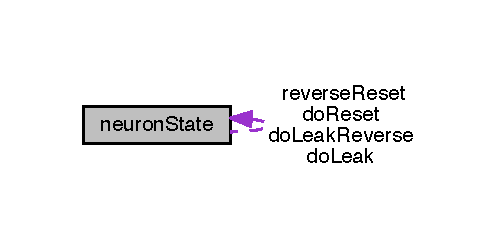
\includegraphics[width=239pt]{structneuron_state__coll__graph}
\end{center}
\end{figure}
\subsection*{Data Fields}
\begin{DoxyCompactItemize}
\item 
\hyperlink{assist_8h_a3f7a6e6a1210b6d9d7a42177dcb9634b}{\+\_\+id\+T} \hyperlink{structneuron_state_a76ef99e5766b6e36c3f41a2920e8c56c}{my\+Core\+I\+D}
\item 
\hyperlink{assist_8h_a3f7a6e6a1210b6d9d7a42177dcb9634b}{\+\_\+id\+T} \hyperlink{structneuron_state_ac24762c24aede292a2ce5df78114881c}{my\+Local\+I\+D}
\begin{DoxyCompactList}\small\item\em Neuron\textquotesingle{}s core\+I\+D. \end{DoxyCompactList}\item 
\hyperlink{assist_8h_abe1fc1b8f9efd1187e564bcb8de7f815}{\+\_\+volt\+T} \hyperlink{structneuron_state_a0fdd8f44c4105a94e17c4c58a51db486}{membrane\+Pot}
\begin{DoxyCompactList}\small\item\em Neuron\textquotesingle{}s local I\+D (from 0 -\/ j-\/1);. \end{DoxyCompactList}\item 
\hyperlink{assist_8h_abe1fc1b8f9efd1187e564bcb8de7f815}{\+\_\+volt\+T} \hyperlink{structneuron_state_ad17e1ac0b4bca75d10da8b0ab56edd6e}{prev\+Membrane\+Pot}
\begin{DoxyCompactList}\small\item\em current \char`\"{}voltage\char`\"{} of neuron \end{DoxyCompactList}\item 
\hyperlink{assist_8h_abe1fc1b8f9efd1187e564bcb8de7f815}{\+\_\+volt\+T} \hyperlink{structneuron_state_af321d0fa58028b78986160845189077e}{threshold}
\begin{DoxyCompactList}\small\item\em previous state membrane potential \end{DoxyCompactList}\item 
tw\+\_\+stime \hyperlink{structneuron_state_a0658ad1f8b57a00589c6ea84f9a4ab13}{last\+Active\+Time}
\begin{DoxyCompactList}\small\item\em neuron\textquotesingle{}s threshold value \end{DoxyCompactList}\item 
uint\+\_\+fast16\+\_\+t \hyperlink{structneuron_state_af8935bcba177f2f3dfb9119c39ef7dc5}{received\+Synapse\+Msgs}
\begin{DoxyCompactList}\small\item\em last time the neuron fired -\/ used for calculating leak and reverse functions. \end{DoxyCompactList}\item 
\hyperlink{neuron_8h_a48885ea6be5b55a2e24de9f97552d4ee}{neuron\+Fire\+Mode} \hyperlink{structneuron_state_a55890f9e021064df30e9d18a9df98845}{fire\+Mode}
\begin{DoxyCompactList}\small\item\em neuron firing parameters \end{DoxyCompactList}\item 
\hyperlink{neuron_8h_ae7e5990745cd949246894bfb633ca4a2}{reset\+Fun\+Del} \hyperlink{structneuron_state_afcf9d931e4fda519c43b4efeab687463}{do\+Reset}
\begin{DoxyCompactList}\small\item\em neuron\textquotesingle{}s firing mode \end{DoxyCompactList}\item 
\hyperlink{assist_8h_abe1fc1b8f9efd1187e564bcb8de7f815}{\+\_\+volt\+T} \hyperlink{structneuron_state_add87cc0b2bc3426f0fd870f7df6decd5}{reset\+Volt\+Param}
\begin{DoxyCompactList}\small\item\em neuron reset function \end{DoxyCompactList}\item 
\hyperlink{neuron_8h_aa939c0acc5b3367975f2f0cb7bc36d17}{reverse\+Reset\+Del} \hyperlink{structneuron_state_abf6970098695585c81e101b2a741b9a5}{reverse\+Reset}
\begin{DoxyCompactList}\small\item\em Optional parameter for reset voltage functions. \end{DoxyCompactList}\item 
\hyperlink{assist_8h_abe1fc1b8f9efd1187e564bcb8de7f815}{\+\_\+volt\+T} $\ast$ \hyperlink{structneuron_state_ab39656a1580505adcabc4c7a1f4d8100}{per\+Synapse\+Weight}
\begin{DoxyCompactList}\small\item\em Neuron reverse reset function. \end{DoxyCompactList}\item 
bool $\ast$ \hyperlink{structneuron_state_a95688135a244a3ce3b35698a49d0da18}{per\+Synapse\+Det}
\begin{DoxyCompactList}\small\item\em An array determining if each synapse is handled stochastically or deterministically. \end{DoxyCompactList}\item 
\hyperlink{assist_8h_a3f7a6e6a1210b6d9d7a42177dcb9634b}{\+\_\+id\+T} \hyperlink{structneuron_state_a62463fa4d33c39297aa5ce3a145d474f}{dendrite\+Core}
\item 
\hyperlink{assist_8h_a3f7a6e6a1210b6d9d7a42177dcb9634b}{\+\_\+id\+T} \hyperlink{structneuron_state_a73e5b16411af572181411b8fd8d5117d}{dendrite\+Local}
\begin{DoxyCompactList}\small\item\em Local core of the remote dendrite. \end{DoxyCompactList}\item 
tw\+\_\+lpid \hyperlink{structneuron_state_a4199c14c5aabfd52f441e01623bdc84c}{dendrite\+Global\+Dest}
\begin{DoxyCompactList}\small\item\em Local I\+D of the remote dendrite -- not L\+P\+I\+D, but a local axon value (0-\/i) \end{DoxyCompactList}\item 
\hyperlink{structleak_fun_del}{leak\+Fun\+Del} \hyperlink{structneuron_state_aa430f424f34dc59dc27736e27ec61320}{do\+Leak}
\begin{DoxyCompactList}\small\item\em G\+I\+D of the axon this neuron talks to. T\+O\+D\+O\+: The dendrite\+Core and dendrite\+Local values might not be needed anymroe. \end{DoxyCompactList}\item 
\hyperlink{structreverse_leak_del}{reverse\+Leak\+Del} \hyperlink{structneuron_state_af4ded7f575b64ada6c0a6664f638307c}{do\+Leak\+Reverse}
\begin{DoxyCompactList}\small\item\em Function pointer to the neuron\textquotesingle{}s current leak function. \end{DoxyCompactList}\item 
\hyperlink{assist_8h_abe1fc1b8f9efd1187e564bcb8de7f815}{\+\_\+volt\+T} \hyperlink{structneuron_state_a7138aaa7e2988e5ad0d32cc9846dcbbb}{leak\+Rate}
\item 
\hyperlink{assist_8h_abe1fc1b8f9efd1187e564bcb8de7f815}{\+\_\+volt\+T} \hyperlink{structneuron_state_a46a71f61511b5311e14643084109d90f}{sgn\+Lambda}
\item 
\hyperlink{assist_8h_ad77e6fc5a9b03d46e7c97b7c4b92e89f}{\+\_\+stat\+T} \hyperlink{structneuron_state_afe8825076c4cf3863c677307fec63c61}{fire\+Count}
\item 
\hyperlink{assist_8h_ad77e6fc5a9b03d46e7c97b7c4b92e89f}{\+\_\+stat\+T} \hyperlink{structneuron_state_ab8f63a1dfdb2992657530ff8a63fdc01}{rcvd\+Msg\+Count}
\begin{DoxyCompactList}\small\item\em count of this neuron\textquotesingle{}s output \end{DoxyCompactList}\item 
\hyperlink{assist_8h_ad77e6fc5a9b03d46e7c97b7c4b92e89f}{\+\_\+stat\+T} \hyperlink{structneuron_state_a71fbb9a79e8048b473b6e09d29a64bbe}{S\+O\+P\+S\+Count}
\begin{DoxyCompactList}\small\item\em The number of synaptic messages received. \end{DoxyCompactList}\end{DoxyCompactItemize}


\subsection{Detailed Description}


Definition at line \hyperlink{neuron_8h_source_l00085}{85} of file \hyperlink{neuron_8h_source}{neuron.\+h}.



\subsection{Field Documentation}
\hypertarget{structneuron_state_a62463fa4d33c39297aa5ce3a145d474f}{}\index{neuron\+State@{neuron\+State}!dendrite\+Core@{dendrite\+Core}}
\index{dendrite\+Core@{dendrite\+Core}!neuron\+State@{neuron\+State}}
\subsubsection[{dendrite\+Core}]{\setlength{\rightskip}{0pt plus 5cm}{\bf \+\_\+id\+T} dendrite\+Core}\label{structneuron_state_a62463fa4d33c39297aa5ce3a145d474f}


Definition at line \hyperlink{neuron_8h_source_l00118}{118} of file \hyperlink{neuron_8h_source}{neuron.\+h}.

\hypertarget{structneuron_state_a4199c14c5aabfd52f441e01623bdc84c}{}\index{neuron\+State@{neuron\+State}!dendrite\+Global\+Dest@{dendrite\+Global\+Dest}}
\index{dendrite\+Global\+Dest@{dendrite\+Global\+Dest}!neuron\+State@{neuron\+State}}
\subsubsection[{dendrite\+Global\+Dest}]{\setlength{\rightskip}{0pt plus 5cm}tw\+\_\+lpid dendrite\+Global\+Dest}\label{structneuron_state_a4199c14c5aabfd52f441e01623bdc84c}


Local I\+D of the remote dendrite -- not L\+P\+I\+D, but a local axon value (0-\/i) 



Definition at line \hyperlink{neuron_8h_source_l00120}{120} of file \hyperlink{neuron_8h_source}{neuron.\+h}.

\hypertarget{structneuron_state_a73e5b16411af572181411b8fd8d5117d}{}\index{neuron\+State@{neuron\+State}!dendrite\+Local@{dendrite\+Local}}
\index{dendrite\+Local@{dendrite\+Local}!neuron\+State@{neuron\+State}}
\subsubsection[{dendrite\+Local}]{\setlength{\rightskip}{0pt plus 5cm}{\bf \+\_\+id\+T} dendrite\+Local}\label{structneuron_state_a73e5b16411af572181411b8fd8d5117d}


Local core of the remote dendrite. 



Definition at line \hyperlink{neuron_8h_source_l00119}{119} of file \hyperlink{neuron_8h_source}{neuron.\+h}.

\hypertarget{structneuron_state_aa430f424f34dc59dc27736e27ec61320}{}\index{neuron\+State@{neuron\+State}!do\+Leak@{do\+Leak}}
\index{do\+Leak@{do\+Leak}!neuron\+State@{neuron\+State}}
\subsubsection[{do\+Leak}]{\setlength{\rightskip}{0pt plus 5cm}{\bf leak\+Fun\+Del} do\+Leak}\label{structneuron_state_aa430f424f34dc59dc27736e27ec61320}


G\+I\+D of the axon this neuron talks to. T\+O\+D\+O\+: The dendrite\+Core and dendrite\+Local values might not be needed anymroe. 



Definition at line \hyperlink{neuron_8h_source_l00123}{123} of file \hyperlink{neuron_8h_source}{neuron.\+h}.

\hypertarget{structneuron_state_af4ded7f575b64ada6c0a6664f638307c}{}\index{neuron\+State@{neuron\+State}!do\+Leak\+Reverse@{do\+Leak\+Reverse}}
\index{do\+Leak\+Reverse@{do\+Leak\+Reverse}!neuron\+State@{neuron\+State}}
\subsubsection[{do\+Leak\+Reverse}]{\setlength{\rightskip}{0pt plus 5cm}{\bf reverse\+Leak\+Del} do\+Leak\+Reverse}\label{structneuron_state_af4ded7f575b64ada6c0a6664f638307c}


Function pointer to the neuron\textquotesingle{}s current leak function. 



Definition at line \hyperlink{neuron_8h_source_l00124}{124} of file \hyperlink{neuron_8h_source}{neuron.\+h}.

\hypertarget{structneuron_state_afcf9d931e4fda519c43b4efeab687463}{}\index{neuron\+State@{neuron\+State}!do\+Reset@{do\+Reset}}
\index{do\+Reset@{do\+Reset}!neuron\+State@{neuron\+State}}
\subsubsection[{do\+Reset}]{\setlength{\rightskip}{0pt plus 5cm}{\bf reset\+Fun\+Del} do\+Reset}\label{structneuron_state_afcf9d931e4fda519c43b4efeab687463}


neuron\textquotesingle{}s firing mode 

neuron reset params 

Definition at line \hyperlink{neuron_8h_source_l00104}{104} of file \hyperlink{neuron_8h_source}{neuron.\+h}.

\hypertarget{structneuron_state_afe8825076c4cf3863c677307fec63c61}{}\index{neuron\+State@{neuron\+State}!fire\+Count@{fire\+Count}}
\index{fire\+Count@{fire\+Count}!neuron\+State@{neuron\+State}}
\subsubsection[{fire\+Count}]{\setlength{\rightskip}{0pt plus 5cm}{\bf \+\_\+stat\+T} fire\+Count}\label{structneuron_state_afe8825076c4cf3863c677307fec63c61}


Definition at line \hyperlink{neuron_8h_source_l00130}{130} of file \hyperlink{neuron_8h_source}{neuron.\+h}.

\hypertarget{structneuron_state_a55890f9e021064df30e9d18a9df98845}{}\index{neuron\+State@{neuron\+State}!fire\+Mode@{fire\+Mode}}
\index{fire\+Mode@{fire\+Mode}!neuron\+State@{neuron\+State}}
\subsubsection[{fire\+Mode}]{\setlength{\rightskip}{0pt plus 5cm}{\bf neuron\+Fire\+Mode} fire\+Mode}\label{structneuron_state_a55890f9e021064df30e9d18a9df98845}


neuron firing parameters 



Definition at line \hyperlink{neuron_8h_source_l00101}{101} of file \hyperlink{neuron_8h_source}{neuron.\+h}.

\hypertarget{structneuron_state_a0658ad1f8b57a00589c6ea84f9a4ab13}{}\index{neuron\+State@{neuron\+State}!last\+Active\+Time@{last\+Active\+Time}}
\index{last\+Active\+Time@{last\+Active\+Time}!neuron\+State@{neuron\+State}}
\subsubsection[{last\+Active\+Time}]{\setlength{\rightskip}{0pt plus 5cm}tw\+\_\+stime last\+Active\+Time}\label{structneuron_state_a0658ad1f8b57a00589c6ea84f9a4ab13}


neuron\textquotesingle{}s threshold value 



Definition at line \hyperlink{neuron_8h_source_l00094}{94} of file \hyperlink{neuron_8h_source}{neuron.\+h}.

\hypertarget{structneuron_state_a7138aaa7e2988e5ad0d32cc9846dcbbb}{}\index{neuron\+State@{neuron\+State}!leak\+Rate@{leak\+Rate}}
\index{leak\+Rate@{leak\+Rate}!neuron\+State@{neuron\+State}}
\subsubsection[{leak\+Rate}]{\setlength{\rightskip}{0pt plus 5cm}{\bf \+\_\+volt\+T} leak\+Rate}\label{structneuron_state_a7138aaa7e2988e5ad0d32cc9846dcbbb}


Definition at line \hyperlink{neuron_8h_source_l00126}{126} of file \hyperlink{neuron_8h_source}{neuron.\+h}.

\hypertarget{structneuron_state_a0fdd8f44c4105a94e17c4c58a51db486}{}\index{neuron\+State@{neuron\+State}!membrane\+Pot@{membrane\+Pot}}
\index{membrane\+Pot@{membrane\+Pot}!neuron\+State@{neuron\+State}}
\subsubsection[{membrane\+Pot}]{\setlength{\rightskip}{0pt plus 5cm}{\bf \+\_\+volt\+T} membrane\+Pot}\label{structneuron_state_a0fdd8f44c4105a94e17c4c58a51db486}


Neuron\textquotesingle{}s local I\+D (from 0 -\/ j-\/1);. 



Definition at line \hyperlink{neuron_8h_source_l00091}{91} of file \hyperlink{neuron_8h_source}{neuron.\+h}.

\hypertarget{structneuron_state_a76ef99e5766b6e36c3f41a2920e8c56c}{}\index{neuron\+State@{neuron\+State}!my\+Core\+I\+D@{my\+Core\+I\+D}}
\index{my\+Core\+I\+D@{my\+Core\+I\+D}!neuron\+State@{neuron\+State}}
\subsubsection[{my\+Core\+I\+D}]{\setlength{\rightskip}{0pt plus 5cm}{\bf \+\_\+id\+T} my\+Core\+I\+D}\label{structneuron_state_a76ef99e5766b6e36c3f41a2920e8c56c}


Definition at line \hyperlink{neuron_8h_source_l00087}{87} of file \hyperlink{neuron_8h_source}{neuron.\+h}.

\hypertarget{structneuron_state_ac24762c24aede292a2ce5df78114881c}{}\index{neuron\+State@{neuron\+State}!my\+Local\+I\+D@{my\+Local\+I\+D}}
\index{my\+Local\+I\+D@{my\+Local\+I\+D}!neuron\+State@{neuron\+State}}
\subsubsection[{my\+Local\+I\+D}]{\setlength{\rightskip}{0pt plus 5cm}{\bf \+\_\+id\+T} my\+Local\+I\+D}\label{structneuron_state_ac24762c24aede292a2ce5df78114881c}


Neuron\textquotesingle{}s core\+I\+D. 



Definition at line \hyperlink{neuron_8h_source_l00088}{88} of file \hyperlink{neuron_8h_source}{neuron.\+h}.

\hypertarget{structneuron_state_a95688135a244a3ce3b35698a49d0da18}{}\index{neuron\+State@{neuron\+State}!per\+Synapse\+Det@{per\+Synapse\+Det}}
\index{per\+Synapse\+Det@{per\+Synapse\+Det}!neuron\+State@{neuron\+State}}
\subsubsection[{per\+Synapse\+Det}]{\setlength{\rightskip}{0pt plus 5cm}bool$\ast$ per\+Synapse\+Det}\label{structneuron_state_a95688135a244a3ce3b35698a49d0da18}


An array determining if each synapse is handled stochastically or deterministically. 

Since the actual hardware has 4 synapse types, this setup has more power than the actual True\+North architecture.

To ensure model $<$-\/$>$ hardware accuracy, at most four different modes should be used per neuron, so that synapses are handled as one of four possible types. 

Definition at line \hyperlink{neuron_8h_source_l00113}{113} of file \hyperlink{neuron_8h_source}{neuron.\+h}.

\hypertarget{structneuron_state_ab39656a1580505adcabc4c7a1f4d8100}{}\index{neuron\+State@{neuron\+State}!per\+Synapse\+Weight@{per\+Synapse\+Weight}}
\index{per\+Synapse\+Weight@{per\+Synapse\+Weight}!neuron\+State@{neuron\+State}}
\subsubsection[{per\+Synapse\+Weight}]{\setlength{\rightskip}{0pt plus 5cm}{\bf \+\_\+volt\+T}$\ast$ per\+Synapse\+Weight}\label{structneuron_state_ab39656a1580505adcabc4c7a1f4d8100}


Neuron reverse reset function. 

In this simulation, each synappse can have a unique weight. In the paper, there is a limit of four different \char`\"{}types\char`\"{} of synapse behavior per neruon. For an accurate sim, there can only be four different values in this array.

Since this is an array, this simulator has the potential to have more power than the actual True\+North hardware architecture. 

Definition at line \hyperlink{neuron_8h_source_l00110}{110} of file \hyperlink{neuron_8h_source}{neuron.\+h}.

\hypertarget{structneuron_state_ad17e1ac0b4bca75d10da8b0ab56edd6e}{}\index{neuron\+State@{neuron\+State}!prev\+Membrane\+Pot@{prev\+Membrane\+Pot}}
\index{prev\+Membrane\+Pot@{prev\+Membrane\+Pot}!neuron\+State@{neuron\+State}}
\subsubsection[{prev\+Membrane\+Pot}]{\setlength{\rightskip}{0pt plus 5cm}{\bf \+\_\+volt\+T} prev\+Membrane\+Pot}\label{structneuron_state_ad17e1ac0b4bca75d10da8b0ab56edd6e}


current \char`\"{}voltage\char`\"{} of neuron 



Definition at line \hyperlink{neuron_8h_source_l00092}{92} of file \hyperlink{neuron_8h_source}{neuron.\+h}.

\hypertarget{structneuron_state_ab8f63a1dfdb2992657530ff8a63fdc01}{}\index{neuron\+State@{neuron\+State}!rcvd\+Msg\+Count@{rcvd\+Msg\+Count}}
\index{rcvd\+Msg\+Count@{rcvd\+Msg\+Count}!neuron\+State@{neuron\+State}}
\subsubsection[{rcvd\+Msg\+Count}]{\setlength{\rightskip}{0pt plus 5cm}{\bf \+\_\+stat\+T} rcvd\+Msg\+Count}\label{structneuron_state_ab8f63a1dfdb2992657530ff8a63fdc01}


count of this neuron\textquotesingle{}s output 



Definition at line \hyperlink{neuron_8h_source_l00131}{131} of file \hyperlink{neuron_8h_source}{neuron.\+h}.

\hypertarget{structneuron_state_af8935bcba177f2f3dfb9119c39ef7dc5}{}\index{neuron\+State@{neuron\+State}!received\+Synapse\+Msgs@{received\+Synapse\+Msgs}}
\index{received\+Synapse\+Msgs@{received\+Synapse\+Msgs}!neuron\+State@{neuron\+State}}
\subsubsection[{received\+Synapse\+Msgs}]{\setlength{\rightskip}{0pt plus 5cm}uint\+\_\+fast16\+\_\+t received\+Synapse\+Msgs}\label{structneuron_state_af8935bcba177f2f3dfb9119c39ef7dc5}


last time the neuron fired -\/ used for calculating leak and reverse functions. 

Used for big-\/tick synchronization. If this neuron has received a synapse message during this big-\/tick cycle, this will be set to $>$ 0. Every synapse received until the big tick occurs will increment this value. Reverse events decrement this value. If the value is == 0 when a synapse message is received, the neuron will send a fire schedule message to itself at the next big-\/tick time. 

Definition at line \hyperlink{neuron_8h_source_l00095}{95} of file \hyperlink{neuron_8h_source}{neuron.\+h}.

\hypertarget{structneuron_state_add87cc0b2bc3426f0fd870f7df6decd5}{}\index{neuron\+State@{neuron\+State}!reset\+Volt\+Param@{reset\+Volt\+Param}}
\index{reset\+Volt\+Param@{reset\+Volt\+Param}!neuron\+State@{neuron\+State}}
\subsubsection[{reset\+Volt\+Param}]{\setlength{\rightskip}{0pt plus 5cm}{\bf \+\_\+volt\+T} reset\+Volt\+Param}\label{structneuron_state_add87cc0b2bc3426f0fd870f7df6decd5}


neuron reset function 



Definition at line \hyperlink{neuron_8h_source_l00105}{105} of file \hyperlink{neuron_8h_source}{neuron.\+h}.

\hypertarget{structneuron_state_abf6970098695585c81e101b2a741b9a5}{}\index{neuron\+State@{neuron\+State}!reverse\+Reset@{reverse\+Reset}}
\index{reverse\+Reset@{reverse\+Reset}!neuron\+State@{neuron\+State}}
\subsubsection[{reverse\+Reset}]{\setlength{\rightskip}{0pt plus 5cm}{\bf reverse\+Reset\+Del} reverse\+Reset}\label{structneuron_state_abf6970098695585c81e101b2a741b9a5}


Optional parameter for reset voltage functions. 



Definition at line \hyperlink{neuron_8h_source_l00107}{107} of file \hyperlink{neuron_8h_source}{neuron.\+h}.

\hypertarget{structneuron_state_a46a71f61511b5311e14643084109d90f}{}\index{neuron\+State@{neuron\+State}!sgn\+Lambda@{sgn\+Lambda}}
\index{sgn\+Lambda@{sgn\+Lambda}!neuron\+State@{neuron\+State}}
\subsubsection[{sgn\+Lambda}]{\setlength{\rightskip}{0pt plus 5cm}{\bf \+\_\+volt\+T} sgn\+Lambda}\label{structneuron_state_a46a71f61511b5311e14643084109d90f}


Definition at line \hyperlink{neuron_8h_source_l00127}{127} of file \hyperlink{neuron_8h_source}{neuron.\+h}.

\hypertarget{structneuron_state_a71fbb9a79e8048b473b6e09d29a64bbe}{}\index{neuron\+State@{neuron\+State}!S\+O\+P\+S\+Count@{S\+O\+P\+S\+Count}}
\index{S\+O\+P\+S\+Count@{S\+O\+P\+S\+Count}!neuron\+State@{neuron\+State}}
\subsubsection[{S\+O\+P\+S\+Count}]{\setlength{\rightskip}{0pt plus 5cm}{\bf \+\_\+stat\+T} S\+O\+P\+S\+Count}\label{structneuron_state_a71fbb9a79e8048b473b6e09d29a64bbe}


The number of synaptic messages received. 



Definition at line \hyperlink{neuron_8h_source_l00132}{132} of file \hyperlink{neuron_8h_source}{neuron.\+h}.

\hypertarget{structneuron_state_af321d0fa58028b78986160845189077e}{}\index{neuron\+State@{neuron\+State}!threshold@{threshold}}
\index{threshold@{threshold}!neuron\+State@{neuron\+State}}
\subsubsection[{threshold}]{\setlength{\rightskip}{0pt plus 5cm}{\bf \+\_\+volt\+T} threshold}\label{structneuron_state_af321d0fa58028b78986160845189077e}


previous state membrane potential 



Definition at line \hyperlink{neuron_8h_source_l00093}{93} of file \hyperlink{neuron_8h_source}{neuron.\+h}.



The documentation for this struct was generated from the following file\+:\begin{DoxyCompactItemize}
\item 
/\+Users/\+Mark/\+Development/\+True\+North/tnt\+\_\+benchmark/models/\hyperlink{neuron_8h}{neuron.\+h}\end{DoxyCompactItemize}

\hypertarget{structrandom_spikes}{}\section{random\+Spikes Struct Reference}
\label{structrandom_spikes}\index{random\+Spikes@{random\+Spikes}}


Struct that genreates spikes randomly.  




{\ttfamily \#include $<$input\+\_\+simulator.\+h$>$}

\subsection*{Data Fields}
\begin{DoxyCompactItemize}
\item 
float \hyperlink{structrandom_spikes_a1333eb5695ae83d1ffccf24b08bc6288}{random\+Rate}
\begin{DoxyCompactList}\small\item\em If the random value is over this, spike. \end{DoxyCompactList}\item 
\hyperlink{input__simulator_8h_aa0d25534cd73156287b1136dd89c0215}{selected\+Random} \hyperlink{structrandom_spikes_a18766f12fc4212349fb61b221f83b779}{rand\+Method}
\begin{DoxyCompactList}\small\item\em Selected random generator. \end{DoxyCompactList}\item 
float \hyperlink{structrandom_spikes_a0eb8199754a403ccc8eac256f9193a02}{rnd\+Fct\+Val}
\begin{DoxyCompactList}\small\item\em For functions that need a second parameter (eg, binomial etc.), this is the second parameter. \end{DoxyCompactList}\end{DoxyCompactItemize}


\subsection{Detailed Description}
Struct that genreates spikes randomly. 



Definition at line \hyperlink{input__simulator_8h_source_l00029}{29} of file \hyperlink{input__simulator_8h_source}{input\+\_\+simulator.\+h}.



\subsection{Field Documentation}
\hypertarget{structrandom_spikes_a18766f12fc4212349fb61b221f83b779}{}\index{random\+Spikes@{random\+Spikes}!rand\+Method@{rand\+Method}}
\index{rand\+Method@{rand\+Method}!random\+Spikes@{random\+Spikes}}
\subsubsection[{rand\+Method}]{\setlength{\rightskip}{0pt plus 5cm}{\bf selected\+Random} rand\+Method}\label{structrandom_spikes_a18766f12fc4212349fb61b221f83b779}


Selected random generator. 



Definition at line \hyperlink{input__simulator_8h_source_l00031}{31} of file \hyperlink{input__simulator_8h_source}{input\+\_\+simulator.\+h}.

\hypertarget{structrandom_spikes_a1333eb5695ae83d1ffccf24b08bc6288}{}\index{random\+Spikes@{random\+Spikes}!random\+Rate@{random\+Rate}}
\index{random\+Rate@{random\+Rate}!random\+Spikes@{random\+Spikes}}
\subsubsection[{random\+Rate}]{\setlength{\rightskip}{0pt plus 5cm}float random\+Rate}\label{structrandom_spikes_a1333eb5695ae83d1ffccf24b08bc6288}


If the random value is over this, spike. 



Definition at line \hyperlink{input__simulator_8h_source_l00030}{30} of file \hyperlink{input__simulator_8h_source}{input\+\_\+simulator.\+h}.

\hypertarget{structrandom_spikes_a0eb8199754a403ccc8eac256f9193a02}{}\index{random\+Spikes@{random\+Spikes}!rnd\+Fct\+Val@{rnd\+Fct\+Val}}
\index{rnd\+Fct\+Val@{rnd\+Fct\+Val}!random\+Spikes@{random\+Spikes}}
\subsubsection[{rnd\+Fct\+Val}]{\setlength{\rightskip}{0pt plus 5cm}float rnd\+Fct\+Val}\label{structrandom_spikes_a0eb8199754a403ccc8eac256f9193a02}


For functions that need a second parameter (eg, binomial etc.), this is the second parameter. 



Definition at line \hyperlink{input__simulator_8h_source_l00032}{32} of file \hyperlink{input__simulator_8h_source}{input\+\_\+simulator.\+h}.



The documentation for this struct was generated from the following file\+:\begin{DoxyCompactItemize}
\item 
/\+Users/\+Mark/\+Development/\+True\+North/tnt\+\_\+benchmark/\hyperlink{input__simulator_8h}{input\+\_\+simulator.\+h}\end{DoxyCompactItemize}

\hypertarget{unionreset_rate}{}\section{reset\+Rate Union Reference}
\label{unionreset_rate}\index{reset\+Rate@{reset\+Rate}}


Reset\+Rate This is a support union for neuron reset rates.  




{\ttfamily \#include $<$neuron.\+h$>$}

\subsection*{Data Fields}
\begin{DoxyCompactItemize}
\item 
int \hyperlink{unionreset_rate_a4bf8a23e4a9874ff73208c681eae1ced}{linear\+Rate}
\item 
float \hyperlink{unionreset_rate_a54aaba14ce85fd9c5d7b385d98727e36}{non\+Linear\+Rate}
\item 
\hyperlink{assist_8h_abe1fc1b8f9efd1187e564bcb8de7f815}{\+\_\+volt\+T} \hyperlink{unionreset_rate_a5a9af6c017d8b70e4db9283f2f7e726b}{volt\+Rate}
\end{DoxyCompactItemize}


\subsection{Detailed Description}
Reset\+Rate This is a support union for neuron reset rates. 



Definition at line \hyperlink{neuron_8h_source_l00080}{80} of file \hyperlink{neuron_8h_source}{neuron.\+h}.



\subsection{Field Documentation}
\hypertarget{unionreset_rate_a4bf8a23e4a9874ff73208c681eae1ced}{}\index{reset\+Rate@{reset\+Rate}!linear\+Rate@{linear\+Rate}}
\index{linear\+Rate@{linear\+Rate}!reset\+Rate@{reset\+Rate}}
\subsubsection[{linear\+Rate}]{\setlength{\rightskip}{0pt plus 5cm}int linear\+Rate}\label{unionreset_rate_a4bf8a23e4a9874ff73208c681eae1ced}


Definition at line \hyperlink{neuron_8h_source_l00081}{81} of file \hyperlink{neuron_8h_source}{neuron.\+h}.

\hypertarget{unionreset_rate_a54aaba14ce85fd9c5d7b385d98727e36}{}\index{reset\+Rate@{reset\+Rate}!non\+Linear\+Rate@{non\+Linear\+Rate}}
\index{non\+Linear\+Rate@{non\+Linear\+Rate}!reset\+Rate@{reset\+Rate}}
\subsubsection[{non\+Linear\+Rate}]{\setlength{\rightskip}{0pt plus 5cm}float non\+Linear\+Rate}\label{unionreset_rate_a54aaba14ce85fd9c5d7b385d98727e36}


Definition at line \hyperlink{neuron_8h_source_l00082}{82} of file \hyperlink{neuron_8h_source}{neuron.\+h}.

\hypertarget{unionreset_rate_a5a9af6c017d8b70e4db9283f2f7e726b}{}\index{reset\+Rate@{reset\+Rate}!volt\+Rate@{volt\+Rate}}
\index{volt\+Rate@{volt\+Rate}!reset\+Rate@{reset\+Rate}}
\subsubsection[{volt\+Rate}]{\setlength{\rightskip}{0pt plus 5cm}{\bf \+\_\+volt\+T} volt\+Rate}\label{unionreset_rate_a5a9af6c017d8b70e4db9283f2f7e726b}


Definition at line \hyperlink{neuron_8h_source_l00083}{83} of file \hyperlink{neuron_8h_source}{neuron.\+h}.



The documentation for this union was generated from the following file\+:\begin{DoxyCompactItemize}
\item 
/home/mplagge/development/tnt\+\_\+benchmark/models/\hyperlink{neuron_8h}{neuron.\+h}\end{DoxyCompactItemize}

\hypertarget{structreverse_leak_del}{}\section{reverse\+Leak\+Del Struct Reference}
\label{structreverse_leak_del}\index{reverse\+Leak\+Del@{reverse\+Leak\+Del}}


This fun.  




{\ttfamily \#include $<$neuron.\+h$>$}



\subsection{Detailed Description}
This fun. 

pointer manages reverse leak functions 

The documentation for this struct was generated from the following file\+:\begin{DoxyCompactItemize}
\item 
/\+Users/\+Mark/\+Development/\+True\+North/tnt\+\_\+benchmark/models/\hyperlink{neuron_8h}{neuron.\+h}\end{DoxyCompactItemize}

\hypertarget{structselected_spikes}{}\section{selected\+Spikes Struct Reference}
\label{structselected_spikes}\index{selected\+Spikes@{selected\+Spikes}}


{\ttfamily \#include $<$input\+\_\+simulator.\+h$>$}

\subsection*{Data Fields}
\begin{DoxyCompactItemize}
\item 
int $\ast$ \hyperlink{structselected_spikes_a666eb9ad96121cf3e4ce134e1a4c12c0}{output\+Mesh}
\begin{DoxyCompactList}\small\item\em Array that represents the output levels per tick. \end{DoxyCompactList}\item 
int \hyperlink{structselected_spikes_a97727a3be0dbd5813f860c99733048a8}{output\+Mesh\+Lengh}
\begin{DoxyCompactList}\small\item\em Size of the output mesh. \end{DoxyCompactList}\end{DoxyCompactItemize}


\subsection{Detailed Description}


Definition at line \hyperlink{input__simulator_8h_source_l00035}{35} of file \hyperlink{input__simulator_8h_source}{input\+\_\+simulator.\+h}.



\subsection{Field Documentation}
\hypertarget{structselected_spikes_a666eb9ad96121cf3e4ce134e1a4c12c0}{}\index{selected\+Spikes@{selected\+Spikes}!output\+Mesh@{output\+Mesh}}
\index{output\+Mesh@{output\+Mesh}!selected\+Spikes@{selected\+Spikes}}
\subsubsection[{output\+Mesh}]{\setlength{\rightskip}{0pt plus 5cm}int$\ast$ output\+Mesh}\label{structselected_spikes_a666eb9ad96121cf3e4ce134e1a4c12c0}


Array that represents the output levels per tick. 



Definition at line \hyperlink{input__simulator_8h_source_l00036}{36} of file \hyperlink{input__simulator_8h_source}{input\+\_\+simulator.\+h}.

\hypertarget{structselected_spikes_a97727a3be0dbd5813f860c99733048a8}{}\index{selected\+Spikes@{selected\+Spikes}!output\+Mesh\+Lengh@{output\+Mesh\+Lengh}}
\index{output\+Mesh\+Lengh@{output\+Mesh\+Lengh}!selected\+Spikes@{selected\+Spikes}}
\subsubsection[{output\+Mesh\+Lengh}]{\setlength{\rightskip}{0pt plus 5cm}int output\+Mesh\+Lengh}\label{structselected_spikes_a97727a3be0dbd5813f860c99733048a8}


Size of the output mesh. 



Definition at line \hyperlink{input__simulator_8h_source_l00037}{37} of file \hyperlink{input__simulator_8h_source}{input\+\_\+simulator.\+h}.



The documentation for this struct was generated from the following file\+:\begin{DoxyCompactItemize}
\item 
/\+Users/\+Mark/\+Development/\+True\+North/tnt\+\_\+benchmark/\hyperlink{input__simulator_8h}{input\+\_\+simulator.\+h}\end{DoxyCompactItemize}

\hypertarget{structsynapse_state}{}\section{synapse\+State Struct Reference}
\label{structsynapse_state}\index{synapse\+State@{synapse\+State}}


{\ttfamily \#include $<$synapse.\+h$>$}



Collaboration diagram for synapse\+State\+:\nopagebreak
\begin{figure}[H]
\begin{center}
\leavevmode
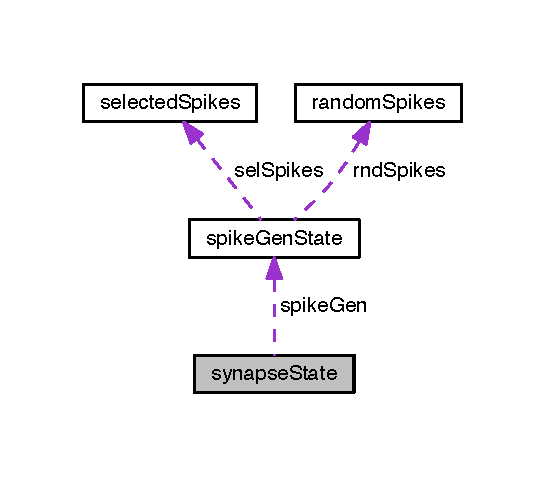
\includegraphics[width=262pt]{structsynapse_state__coll__graph}
\end{center}
\end{figure}
\subsection*{Data Fields}
\begin{DoxyCompactItemize}
\item 
unsigned int \hyperlink{structsynapse_state_aef661be02823d13d471c66bf0cd478db}{syn\+I\+D}
\item 
unsigned int \hyperlink{structsynapse_state_a2063050696509e31bdd72dbb0607c6ee}{core\+I\+D}
\item 
tw\+\_\+lpid $\ast$ \hyperlink{structsynapse_state_a6d6a80692ca06baa6c9a11a624129763}{dests}
\item 
\hyperlink{structspike_gen_state}{spike\+Gen\+State} $\ast$ \hyperlink{structsynapse_state_a11fd4dc41f715eb6f04a68bc5fc9e292}{spike\+Gen}
\end{DoxyCompactItemize}


\subsection{Detailed Description}


Definition at line 17 of file synapse.\+h.



\subsection{Field Documentation}
\hypertarget{structsynapse_state_a2063050696509e31bdd72dbb0607c6ee}{}\index{synapse\+State@{synapse\+State}!core\+I\+D@{core\+I\+D}}
\index{core\+I\+D@{core\+I\+D}!synapse\+State@{synapse\+State}}
\subsubsection[{core\+I\+D}]{\setlength{\rightskip}{0pt plus 5cm}unsigned int core\+I\+D}\label{structsynapse_state_a2063050696509e31bdd72dbb0607c6ee}


Definition at line 19 of file synapse.\+h.

\hypertarget{structsynapse_state_a6d6a80692ca06baa6c9a11a624129763}{}\index{synapse\+State@{synapse\+State}!dests@{dests}}
\index{dests@{dests}!synapse\+State@{synapse\+State}}
\subsubsection[{dests}]{\setlength{\rightskip}{0pt plus 5cm}tw\+\_\+lpid$\ast$ dests}\label{structsynapse_state_a6d6a80692ca06baa6c9a11a624129763}


Definition at line 20 of file synapse.\+h.

\hypertarget{structsynapse_state_a11fd4dc41f715eb6f04a68bc5fc9e292}{}\index{synapse\+State@{synapse\+State}!spike\+Gen@{spike\+Gen}}
\index{spike\+Gen@{spike\+Gen}!synapse\+State@{synapse\+State}}
\subsubsection[{spike\+Gen}]{\setlength{\rightskip}{0pt plus 5cm}{\bf spike\+Gen\+State}$\ast$ spike\+Gen}\label{structsynapse_state_a11fd4dc41f715eb6f04a68bc5fc9e292}


Definition at line 22 of file synapse.\+h.

\hypertarget{structsynapse_state_aef661be02823d13d471c66bf0cd478db}{}\index{synapse\+State@{synapse\+State}!syn\+I\+D@{syn\+I\+D}}
\index{syn\+I\+D@{syn\+I\+D}!synapse\+State@{synapse\+State}}
\subsubsection[{syn\+I\+D}]{\setlength{\rightskip}{0pt plus 5cm}unsigned int syn\+I\+D}\label{structsynapse_state_aef661be02823d13d471c66bf0cd478db}


Definition at line 18 of file synapse.\+h.



The documentation for this struct was generated from the following file\+:\begin{DoxyCompactItemize}
\item 
/\+Users/\+Mark/\+Development/\+True\+North/tnt\+\_\+benchmark/models/\hyperlink{synapse_8h}{synapse.\+h}\end{DoxyCompactItemize}

\chapter{File Documentation}
\hypertarget{assist_8c}{}\section{/home/mplagge/development/tnt\+\_\+benchmark/assist.c File Reference}
\label{assist_8c}\index{/home/mplagge/development/tnt\+\_\+benchmark/assist.\+c@{/home/mplagge/development/tnt\+\_\+benchmark/assist.\+c}}
{\ttfamily \#include \char`\"{}assist.\+h\char`\"{}}\\*
{\ttfamily \#include $<$math.\+h$>$}\\*
Include dependency graph for assist.\+c\+:\nopagebreak
\begin{figure}[H]
\begin{center}
\leavevmode
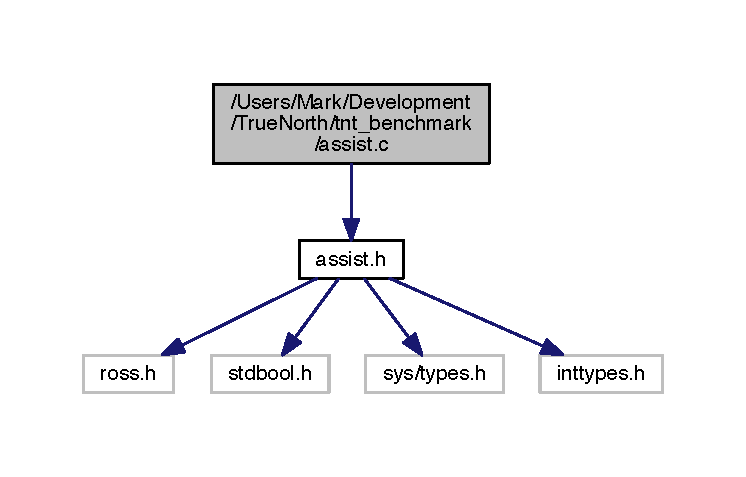
\includegraphics[width=340pt]{assist_8c__incl}
\end{center}
\end{figure}
\subsection*{Functions}
\begin{DoxyCompactItemize}
\item 
tw\+\_\+stime \hyperlink{assist_8c_a30602b11dbfa6bcb90dc00e7942cfb02}{get\+Next\+Event\+Time} (tw\+\_\+lp $\ast$lp)
\begin{DoxyCompactList}\small\item\em Gets the next small-\/tick event time. \end{DoxyCompactList}\item 
tw\+\_\+stime \hyperlink{assist_8c_a4d378196b7fceed090d64ec8820b4065}{get\+Current\+Big\+Tick} (tw\+\_\+stime now)
\begin{DoxyCompactList}\small\item\em Given a tw\+\_\+stime, returns the current big tick. \end{DoxyCompactList}\item 
tw\+\_\+stime \hyperlink{assist_8c_aa961bc9b414f1429b123fc8212c989fd}{get\+Next\+Big\+Tick} (tw\+\_\+stime now)
\begin{DoxyCompactList}\small\item\em Given a tw\+\_\+stime, returns the next big-\/tick that will happen. \end{DoxyCompactList}\end{DoxyCompactItemize}


\subsection{Function Documentation}
\hypertarget{assist_8c_a4d378196b7fceed090d64ec8820b4065}{}\index{assist.\+c@{assist.\+c}!get\+Current\+Big\+Tick@{get\+Current\+Big\+Tick}}
\index{get\+Current\+Big\+Tick@{get\+Current\+Big\+Tick}!assist.\+c@{assist.\+c}}
\subsubsection[{get\+Current\+Big\+Tick}]{\setlength{\rightskip}{0pt plus 5cm}tw\+\_\+stime get\+Current\+Big\+Tick (
\begin{DoxyParamCaption}
\item[{tw\+\_\+stime}]{now}
\end{DoxyParamCaption}
)}\label{assist_8c_a4d378196b7fceed090d64ec8820b4065}


Given a tw\+\_\+stime, returns the current big tick. 

If the time is in-\/between big ticks, this rounds down to the last big tick. There is a bit of a fuzz for times close to the next big tick so if the current time is within \hyperlink{assist_8h_a69434dbcf2196fc2fd1ab7cb57fc9491}{B\+I\+G\+\_\+\+T\+I\+C\+K\+\_\+\+E\+R\+R} of the next big tick, that will be returned instead. Sane parameters would probably be around .000001.\begin{DoxyRefDesc}{Todo}
\item[\hyperlink{todo__todo000001}{Todo}]\+: Implement \& determin if ε needs to be added to the return value.\end{DoxyRefDesc}
\begin{DoxyRefDesc}{Todo}
\item[\hyperlink{todo__todo000002}{Todo}]need to see if this will kill performance\+: \end{DoxyRefDesc}


Definition at line \hyperlink{assist_8c_source_l00030}{30} of file \hyperlink{assist_8c_source}{assist.\+c}.



References \hyperlink{model__main_8h_source_l00063}{C\+O\+R\+E\+\_\+\+S\+I\+Z\+E}.



Referenced by \hyperlink{assist_8c_source_l00041}{get\+Next\+Big\+Tick()}, and \hyperlink{neuron_8c_source_l00028}{linear\+Leak()}.


\begin{DoxyCode}
00030                                         \{
00031     tw\_stime ctick = now / \hyperlink{assist_8h_ad39b86a0b748731175572436f6672264}{CORE\_SIZE};
00033     \textcolor{keywordtype}{long} \textcolor{keywordtype}{double} vtr = 0;
00034     \textcolor{keywordtype}{long} \textcolor{keywordtype}{long} rem = modfl(ctick, &vtr);
00035     \textcolor{comment}{//Rem is current tick, vtr is offset.}
00036 
00037     \textcolor{keywordflow}{return} rem;
00038 
00039 \}
\end{DoxyCode}
\hypertarget{assist_8c_aa961bc9b414f1429b123fc8212c989fd}{}\index{assist.\+c@{assist.\+c}!get\+Next\+Big\+Tick@{get\+Next\+Big\+Tick}}
\index{get\+Next\+Big\+Tick@{get\+Next\+Big\+Tick}!assist.\+c@{assist.\+c}}
\subsubsection[{get\+Next\+Big\+Tick}]{\setlength{\rightskip}{0pt plus 5cm}tw\+\_\+stime get\+Next\+Big\+Tick (
\begin{DoxyParamCaption}
\item[{tw\+\_\+stime}]{now}
\end{DoxyParamCaption}
)}\label{assist_8c_aa961bc9b414f1429b123fc8212c989fd}


Given a tw\+\_\+stime, returns the next big-\/tick that will happen. 


\begin{DoxyParams}{Parameters}
{\em now} & Right now!\\
\hline
\end{DoxyParams}
\begin{DoxyReturn}{Returns}
Next big tick time. 
\end{DoxyReturn}


Definition at line \hyperlink{assist_8c_source_l00041}{41} of file \hyperlink{assist_8c_source}{assist.\+c}.



References \hyperlink{model__main_8h_source_l00063}{C\+O\+R\+E\+\_\+\+S\+I\+Z\+E}, and \hyperlink{assist_8c_source_l00030}{get\+Current\+Big\+Tick()}.



Referenced by \hyperlink{neuron_8c_source_l00167}{neuron\+Fire()}, and \hyperlink{neuron_8c_source_l00179}{send\+Heartbeat()}.


\begin{DoxyCode}
00041                                       \{
00042     \textcolor{keywordtype}{long} \textcolor{keywordtype}{long} curr = \hyperlink{assist_8h_ad39b86a0b748731175572436f6672264}{CORE\_SIZE} * \hyperlink{assist_8c_a4d378196b7fceed090d64ec8820b4065}{getCurrentBigTick}(now) + 1;
00043     \textcolor{keywordflow}{return} curr - now;
00044 
00045         \textcolor{comment}{//Need to figure this out - not accurate until this is done:}
00046 
00047 \}\end{DoxyCode}


Here is the call graph for this function\+:\nopagebreak
\begin{figure}[H]
\begin{center}
\leavevmode
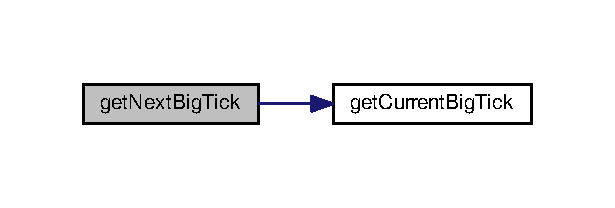
\includegraphics[width=295pt]{assist_8c_aa961bc9b414f1429b123fc8212c989fd_cgraph}
\end{center}
\end{figure}


\hypertarget{assist_8c_a30602b11dbfa6bcb90dc00e7942cfb02}{}\index{assist.\+c@{assist.\+c}!get\+Next\+Event\+Time@{get\+Next\+Event\+Time}}
\index{get\+Next\+Event\+Time@{get\+Next\+Event\+Time}!assist.\+c@{assist.\+c}}
\subsubsection[{get\+Next\+Event\+Time}]{\setlength{\rightskip}{0pt plus 5cm}tw\+\_\+stime get\+Next\+Event\+Time (
\begin{DoxyParamCaption}
\item[{tw\+\_\+lp $\ast$}]{lp}
\end{DoxyParamCaption}
)}\label{assist_8c_a30602b11dbfa6bcb90dc00e7942cfb02}


Gets the next small-\/tick event time. 

Gets the next event time, based on a random function. 

Definition at line \hyperlink{assist_8c_source_l00014}{14} of file \hyperlink{assist_8c_source}{assist.\+c}.



Referenced by \hyperlink{axon_8c_source_l00011}{axon\+Receive\+Message()}, and \hyperlink{synapse_8c_source_l00011}{synapse\+Receive\+Message()}.


\begin{DoxyCode}
00014                                     \{
00015 
00016     tw\_stime r =tw\_rand\_unif(lp->rng) / 10;
00017 
00018     \textcolor{keywordflow}{return} r;
00019 
00020 \}
\end{DoxyCode}

\hypertarget{assist_8c_source}{}\section{/\+Users/\+Mark/\+Development/\+True\+North/tnt\+\_\+benchmark/assist.c}

\begin{DoxyCode}
00001 \textcolor{comment}{//}
00002 \textcolor{comment}{//  assist.c}
00003 \textcolor{comment}{//  ROSS\_TOP}
00004 \textcolor{comment}{//}
00005 \textcolor{comment}{//  Created by Mark Plagge on 6/17/15.}
00006 \textcolor{comment}{//}
00007 \textcolor{comment}{//}
00008 
00009 \textcolor{preprocessor}{#}\textcolor{preprocessor}{include} \hyperlink{assist_8h}{"assist.h"}
00010 \textcolor{comment}{/**}
00011 \textcolor{comment}{ *  Gets the next event time, based on a random function. Moved here to allow for}
00012 \textcolor{comment}{ *  easier abstraciton, and random function replacement.}
00013 \textcolor{comment}{ *}
00014 \textcolor{comment}{ *}
00015 \textcolor{comment}{ *  @param lp Reference to the current LP so that the function can see the RNG}
00016 \textcolor{comment}{ *}
00017 \textcolor{comment}{ *  @return a tw\_stime value, such that \(\backslash\)f$ 0 < t < 1 \(\backslash\)f$. A delta for the next}
00018 \textcolor{comment}{ *  time slice.}
00019 \textcolor{comment}{ */}
\hypertarget{assist_8c_source_l00020}{}\hyperlink{assist_8h_a30602b11dbfa6bcb90dc00e7942cfb02}{00020} \hyperlink{assist_8h_a30602b11dbfa6bcb90dc00e7942cfb02}{tw\_stime} \hyperlink{assist_8h_a30602b11dbfa6bcb90dc00e7942cfb02}{getNextEventTime}(\hyperlink{assist_8h_a30602b11dbfa6bcb90dc00e7942cfb02}{tw\_lp} *\hyperlink{assist_8h_a30602b11dbfa6bcb90dc00e7942cfb02}{lp})\{
00021 
00022     tw\_stime r =tw\_rand\_unif(lp->rng) / 10;
00023 
00024     \textcolor{keywordflow}{return} r;
00025 
00026 \}
\end{DoxyCode}

\hypertarget{assist_8h}{}\section{/\+Users/\+Mark/\+Development/\+True\+North/tnt\+\_\+benchmark/assist.h File Reference}
\label{assist_8h}\index{/\+Users/\+Mark/\+Development/\+True\+North/tnt\+\_\+benchmark/assist.\+h@{/\+Users/\+Mark/\+Development/\+True\+North/tnt\+\_\+benchmark/assist.\+h}}
{\ttfamily \#include $<$stdio.\+h$>$}\\*
{\ttfamily \#include $<$inttypes.\+h$>$}\\*
{\ttfamily \#include $<$stdbool.\+h$>$}\\*
{\ttfamily \#include \char`\"{}ross.\+h\char`\"{}}\\*
Include dependency graph for assist.\+h\+:
\nopagebreak
\begin{figure}[H]
\begin{center}
\leavevmode
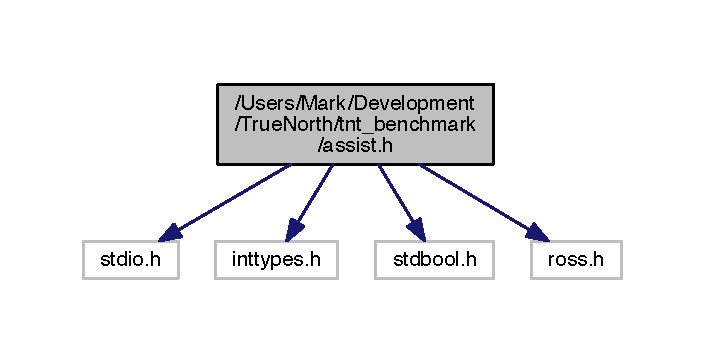
\includegraphics[width=338pt]{assist_8h__incl}
\end{center}
\end{figure}
This graph shows which files directly or indirectly include this file\+:
\nopagebreak
\begin{figure}[H]
\begin{center}
\leavevmode
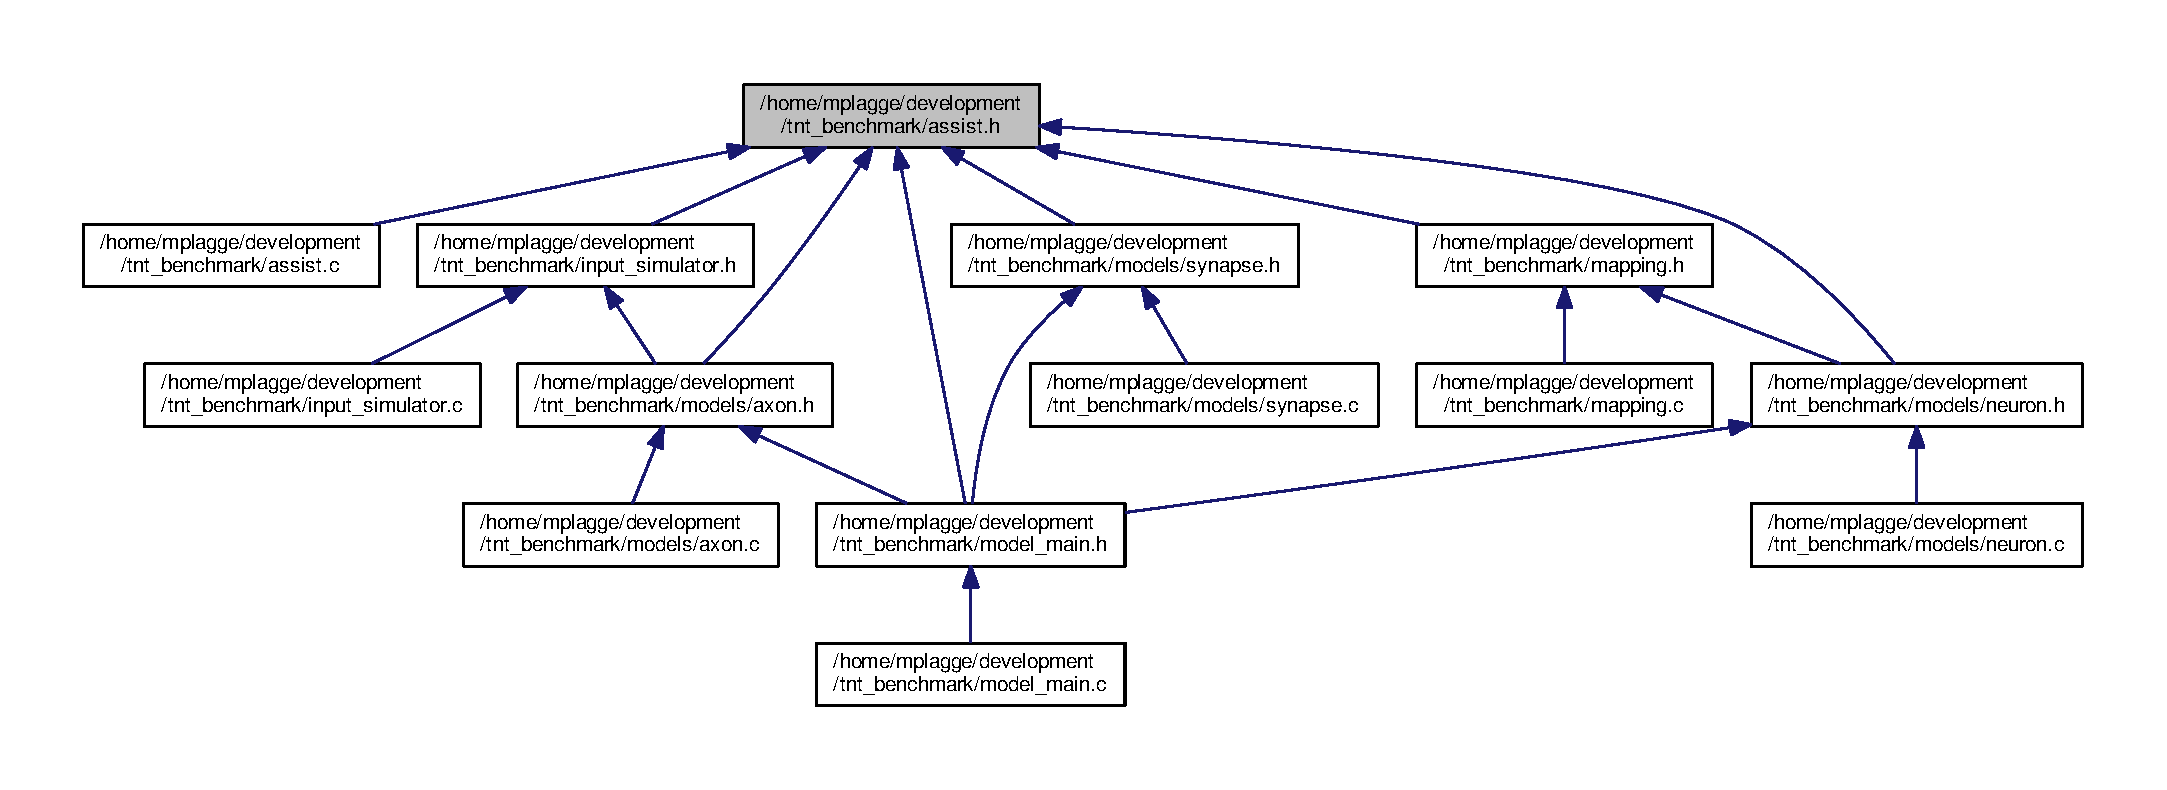
\includegraphics[width=350pt]{assist_8h__dep__incl}
\end{center}
\end{figure}
\subsection*{Data Structures}
\begin{DoxyCompactItemize}
\item 
struct \hyperlink{struct_msg___data}{Msg\+\_\+\+Data}
\begin{DoxyCompactList}\small\item\em Main message struct. \end{DoxyCompactList}\end{DoxyCompactItemize}
\subsection*{Macros}
\begin{DoxyCompactItemize}
\item 
\#define \hyperlink{assist_8h_a3f7a6e6a1210b6d9d7a42177dcb9634b}{\+\_\+id\+T}~uint\+\_\+fast32\+\_\+t
\item 
\#define \hyperlink{assist_8h_abe1fc1b8f9efd1187e564bcb8de7f815}{\+\_\+volt\+T}~int\+\_\+fast32\+\_\+t
\item 
\#define \hyperlink{assist_8h_ad77e6fc5a9b03d46e7c97b7c4b92e89f}{\+\_\+stat\+T}~int\+\_\+fast64\+\_\+t
\item 
\#define \hyperlink{assist_8h_abd3130ec511af0cc7768768554bd36a0}{\+\_\+reg\+I\+D\+T}~uint32\+\_\+t
\begin{DoxyCompactList}\small\item\em \+\_\+reg\+I\+D\+T is a \char`\"{}regional id\char`\"{} type. \end{DoxyCompactList}\item 
\#define \hyperlink{assist_8h_aaf4b596256d346dd40bc6f14c3eb9371}{I\+A\+B\+S}(a)~(((a) $<$ 0) ? (-\/a) \+: (a))
\begin{DoxyCompactList}\small\item\em I\+A\+B\+S is an integer absolute value function. \end{DoxyCompactList}\item 
\#define \hyperlink{assist_8h_ad383c153e77508e2556003da0e4ac3eb}{R\+Z\+E\+R}(a)~(((a) $<$ 0) ? (0) \+: (a))
\begin{DoxyCompactList}\small\item\em R\+Z\+E\+R is a floor function -\/ values below zero round up to zero. \end{DoxyCompactList}\end{DoxyCompactItemize}
\subsection*{Enumerations}
\begin{DoxyCompactItemize}
\item 
enum \hyperlink{assist_8h_a7c1688de451e0dea1e11617bce3ec450}{evt\+Type} \{ \\*
\hyperlink{assist_8h_a7c1688de451e0dea1e11617bce3ec450abb8b28588ca2e1c33d29df003b3b90ee}{A\+X\+O\+N\+\_\+\+O\+U\+T}, 
\hyperlink{assist_8h_a7c1688de451e0dea1e11617bce3ec450a9afa7ee7839cdd980f348a3a70b0054f}{A\+X\+O\+N\+\_\+\+H\+E\+A\+R\+T\+B\+E\+A\+T}, 
\hyperlink{assist_8h_a7c1688de451e0dea1e11617bce3ec450a6ad6b93d8a818550e7246f6e0d143afb}{S\+Y\+N\+A\+P\+S\+E\+\_\+\+O\+U\+T}, 
\hyperlink{assist_8h_a7c1688de451e0dea1e11617bce3ec450a777cedd6ca25a5d7a84aab10a8735af0}{N\+E\+U\+R\+O\+N\+\_\+\+O\+U\+T}, 
\\*
\hyperlink{assist_8h_a7c1688de451e0dea1e11617bce3ec450a226690009a653238a52339561e6c466e}{N\+E\+U\+R\+O\+N\+\_\+\+H\+E\+A\+R\+T\+B\+E\+A\+T}, 
\hyperlink{assist_8h_a7c1688de451e0dea1e11617bce3ec450add78176054e14835c454b5f2d1827d42}{G\+E\+N\+\_\+\+H\+E\+A\+R\+T\+B\+E\+A\+T}
 \}
\begin{DoxyCompactList}\small\item\em evt\+Type is a message/event identifier flag \end{DoxyCompactList}\end{DoxyCompactItemize}
\subsection*{Functions}
\begin{DoxyCompactItemize}
\item 
tw\+\_\+stime \hyperlink{assist_8h_a30602b11dbfa6bcb90dc00e7942cfb02}{get\+Next\+Event\+Time} (tw\+\_\+lp $\ast$lp)
\begin{DoxyCompactList}\small\item\em Gets the next event time, based on a random function. \end{DoxyCompactList}\end{DoxyCompactItemize}
\subsection*{Variables}
\begin{DoxyCompactItemize}
\item 
int \hyperlink{assist_8h_a67e8e45768f76b984a60fcff2b7c51aa}{N\+E\+U\+R\+O\+N\+S\+\_\+\+I\+N\+\_\+\+C\+O\+R\+E}
\begin{DoxyCompactList}\small\item\em Number of neurons per core. \end{DoxyCompactList}\item 
int \hyperlink{assist_8h_a142b2655c5a899956164ef4e1c394fea}{C\+O\+R\+E\+S\+\_\+\+I\+N\+\_\+\+S\+I\+M}
\item 
int \hyperlink{assist_8h_a519a06367b2b3f793c56d3ab78f5b2ef}{A\+X\+O\+N\+S\+\_\+\+I\+N\+\_\+\+C\+O\+R\+E}
\begin{DoxyCompactList}\small\item\em Number of axions per core. \end{DoxyCompactList}\item 
int \hyperlink{assist_8h_a076b99099b46431255982b2bb8ce06fb}{S\+Y\+N\+A\+P\+S\+E\+S\+\_\+\+I\+N\+\_\+\+C\+O\+R\+E}
\item 
unsigned int \hyperlink{assist_8h_a74019486208bb1d640927710d5344a94}{G\+E\+N\+\_\+\+O\+N}
\begin{DoxyCompactList}\small\item\em Simulation tuning variables. \end{DoxyCompactList}\item 
bool \hyperlink{assist_8h_ab42fd7d6d043114d1147acc77bd7e867}{G\+E\+N\+\_\+\+R\+N\+D}
\item 
unsigned int \hyperlink{assist_8h_a516f1496efbe86dedb0e2883bb7e7834}{R\+N\+D\+\_\+\+M\+O\+D\+E}
\item 
unsigned int \hyperlink{assist_8h_a4875b976acd12ff43cc03898be994253}{G\+E\+N\+\_\+\+P\+R\+O\+B}
\item 
unsigned int \hyperlink{assist_8h_a3ba8de640782035ea9e91ab791d9f14f}{G\+E\+N\+\_\+\+F\+C\+T}
\item 
unsigned int \hyperlink{assist_8h_a6f8efb1b6d497ba57f27acadae57dc4b}{G\+E\+N\+\_\+\+O\+U\+T\+B\+O\+U\+N\+D}
\item 
unsigned int \hyperlink{assist_8h_ab161ae8a99d41559eba4ab3dd8d69218}{G\+E\+N\+\_\+\+S\+E\+L\+\_\+\+M\+O\+D\+E}
\item 
unsigned int \hyperlink{assist_8h_a0a9f8592bd29be6c5c7433c3c0bf42dd}{S\+P\+\_\+\+D\+B\+G}
\item 
int \hyperlink{assist_8h_a433873baf41da436ba9c1734c8c5ddd2}{T\+H\+R\+E\+S\+H\+O\+L\+D\+\_\+\+M\+A\+X}
\begin{DoxyCompactList}\small\item\em Determines the maximum and minimum thresholds for a neuron to fire. \end{DoxyCompactList}\item 
int \hyperlink{assist_8h_a55f4484944f4174b5e677c0a71b30e4a}{T\+H\+R\+E\+S\+H\+O\+L\+D\+\_\+\+M\+I\+N}
\begin{DoxyCompactList}\small\item\em Minimum threshold. \end{DoxyCompactList}\item 
int \hyperlink{assist_8h_a20ef6d41d2f384358522fb59fb6226cb}{S\+Y\+N\+A\+P\+S\+E\+\_\+\+W\+E\+I\+G\+H\+T\+\_\+\+M\+A\+X}
\begin{DoxyCompactList}\small\item\em Each neuron is connected to the synapses (inputs) within the core it is running in. \end{DoxyCompactList}\item 
int \hyperlink{assist_8h_af38a0e2e2483ef81f7ea5175c366ce82}{S\+Y\+N\+A\+P\+S\+E\+\_\+\+W\+E\+I\+G\+H\+T\+\_\+\+M\+I\+N}
\begin{DoxyCompactList}\small\item\em Minimum synapse weight. \end{DoxyCompactList}\item 
int \hyperlink{assist_8h_ad39b86a0b748731175572436f6672264}{C\+O\+R\+E\+\_\+\+S\+I\+Z\+E}
\begin{DoxyCompactList}\small\item\em C\+O\+R\+E\+\_\+\+S\+I\+Z\+E is equal to the number of axions $\ast$ number of aneurons + num neurons + num axions. \end{DoxyCompactList}\end{DoxyCompactItemize}


\subsection{Macro Definition Documentation}
\hypertarget{assist_8h_a3f7a6e6a1210b6d9d7a42177dcb9634b}{}\index{assist.\+h@{assist.\+h}!\+\_\+id\+T@{\+\_\+id\+T}}
\index{\+\_\+id\+T@{\+\_\+id\+T}!assist.\+h@{assist.\+h}}
\subsubsection[{\+\_\+id\+T}]{\setlength{\rightskip}{0pt plus 5cm}\#define \+\_\+id\+T~uint\+\_\+fast32\+\_\+t}\label{assist_8h_a3f7a6e6a1210b6d9d7a42177dcb9634b}


Definition at line \hyperlink{assist_8h_source_l00018}{18} of file \hyperlink{assist_8h_source}{assist.\+h}.

\hypertarget{assist_8h_abd3130ec511af0cc7768768554bd36a0}{}\index{assist.\+h@{assist.\+h}!\+\_\+reg\+I\+D\+T@{\+\_\+reg\+I\+D\+T}}
\index{\+\_\+reg\+I\+D\+T@{\+\_\+reg\+I\+D\+T}!assist.\+h@{assist.\+h}}
\subsubsection[{\+\_\+reg\+I\+D\+T}]{\setlength{\rightskip}{0pt plus 5cm}\#define \+\_\+reg\+I\+D\+T~uint32\+\_\+t}\label{assist_8h_abd3130ec511af0cc7768768554bd36a0}


\+\_\+reg\+I\+D\+T is a \char`\"{}regional id\char`\"{} type. 

This variable type is for storing core\+I\+Ds and local\+I\+Ds. It must be half the bit size of tw\+\_\+lpid.\begin{DoxyRefDesc}{Todo}
\item[\hyperlink{todo__todo000001}{Todo}]\+: add macro to adjust the bit width. \end{DoxyRefDesc}


Definition at line \hyperlink{assist_8h_source_l00024}{24} of file \hyperlink{assist_8h_source}{assist.\+h}.

\hypertarget{assist_8h_ad77e6fc5a9b03d46e7c97b7c4b92e89f}{}\index{assist.\+h@{assist.\+h}!\+\_\+stat\+T@{\+\_\+stat\+T}}
\index{\+\_\+stat\+T@{\+\_\+stat\+T}!assist.\+h@{assist.\+h}}
\subsubsection[{\+\_\+stat\+T}]{\setlength{\rightskip}{0pt plus 5cm}\#define \+\_\+stat\+T~int\+\_\+fast64\+\_\+t}\label{assist_8h_ad77e6fc5a9b03d46e7c97b7c4b92e89f}


Definition at line \hyperlink{assist_8h_source_l00020}{20} of file \hyperlink{assist_8h_source}{assist.\+h}.

\hypertarget{assist_8h_abe1fc1b8f9efd1187e564bcb8de7f815}{}\index{assist.\+h@{assist.\+h}!\+\_\+volt\+T@{\+\_\+volt\+T}}
\index{\+\_\+volt\+T@{\+\_\+volt\+T}!assist.\+h@{assist.\+h}}
\subsubsection[{\+\_\+volt\+T}]{\setlength{\rightskip}{0pt plus 5cm}\#define \+\_\+volt\+T~int\+\_\+fast32\+\_\+t}\label{assist_8h_abe1fc1b8f9efd1187e564bcb8de7f815}


Definition at line \hyperlink{assist_8h_source_l00019}{19} of file \hyperlink{assist_8h_source}{assist.\+h}.

\hypertarget{assist_8h_aaf4b596256d346dd40bc6f14c3eb9371}{}\index{assist.\+h@{assist.\+h}!I\+A\+B\+S@{I\+A\+B\+S}}
\index{I\+A\+B\+S@{I\+A\+B\+S}!assist.\+h@{assist.\+h}}
\subsubsection[{I\+A\+B\+S}]{\setlength{\rightskip}{0pt plus 5cm}\#define I\+A\+B\+S(
\begin{DoxyParamCaption}
\item[{}]{a}
\end{DoxyParamCaption}
)~(((a) $<$ 0) ? (-\/a) \+: (a))}\label{assist_8h_aaf4b596256d346dd40bc6f14c3eb9371}


I\+A\+B\+S is an integer absolute value function. 



Definition at line \hyperlink{assist_8h_source_l00029}{29} of file \hyperlink{assist_8h_source}{assist.\+h}.

\hypertarget{assist_8h_ad383c153e77508e2556003da0e4ac3eb}{}\index{assist.\+h@{assist.\+h}!R\+Z\+E\+R@{R\+Z\+E\+R}}
\index{R\+Z\+E\+R@{R\+Z\+E\+R}!assist.\+h@{assist.\+h}}
\subsubsection[{R\+Z\+E\+R}]{\setlength{\rightskip}{0pt plus 5cm}\#define R\+Z\+E\+R(
\begin{DoxyParamCaption}
\item[{}]{a}
\end{DoxyParamCaption}
)~(((a) $<$ 0) ? (0) \+: (a))}\label{assist_8h_ad383c153e77508e2556003da0e4ac3eb}


R\+Z\+E\+R is a floor function -\/ values below zero round up to zero. 



Definition at line \hyperlink{assist_8h_source_l00031}{31} of file \hyperlink{assist_8h_source}{assist.\+h}.



\subsection{Enumeration Type Documentation}
\hypertarget{assist_8h_a7c1688de451e0dea1e11617bce3ec450}{}\index{assist.\+h@{assist.\+h}!evt\+Type@{evt\+Type}}
\index{evt\+Type@{evt\+Type}!assist.\+h@{assist.\+h}}
\subsubsection[{evt\+Type}]{\setlength{\rightskip}{0pt plus 5cm}enum {\bf evt\+Type}}\label{assist_8h_a7c1688de451e0dea1e11617bce3ec450}


evt\+Type is a message/event identifier flag 

\begin{Desc}
\item[Enumerator]\par
\begin{description}
\index{A\+X\+O\+N\+\_\+\+O\+U\+T@{A\+X\+O\+N\+\_\+\+O\+U\+T}!assist.\+h@{assist.\+h}}\index{assist.\+h@{assist.\+h}!A\+X\+O\+N\+\_\+\+O\+U\+T@{A\+X\+O\+N\+\_\+\+O\+U\+T}}\item[{\em 
\hypertarget{assist_8h_a7c1688de451e0dea1e11617bce3ec450abb8b28588ca2e1c33d29df003b3b90ee}{}A\+X\+O\+N\+\_\+\+O\+U\+T\label{assist_8h_a7c1688de451e0dea1e11617bce3ec450abb8b28588ca2e1c33d29df003b3b90ee}
}]\index{A\+X\+O\+N\+\_\+\+H\+E\+A\+R\+T\+B\+E\+A\+T@{A\+X\+O\+N\+\_\+\+H\+E\+A\+R\+T\+B\+E\+A\+T}!assist.\+h@{assist.\+h}}\index{assist.\+h@{assist.\+h}!A\+X\+O\+N\+\_\+\+H\+E\+A\+R\+T\+B\+E\+A\+T@{A\+X\+O\+N\+\_\+\+H\+E\+A\+R\+T\+B\+E\+A\+T}}\item[{\em 
\hypertarget{assist_8h_a7c1688de451e0dea1e11617bce3ec450a9afa7ee7839cdd980f348a3a70b0054f}{}A\+X\+O\+N\+\_\+\+H\+E\+A\+R\+T\+B\+E\+A\+T\label{assist_8h_a7c1688de451e0dea1e11617bce3ec450a9afa7ee7839cdd980f348a3a70b0054f}
}]Message originates from an axon. \index{S\+Y\+N\+A\+P\+S\+E\+\_\+\+O\+U\+T@{S\+Y\+N\+A\+P\+S\+E\+\_\+\+O\+U\+T}!assist.\+h@{assist.\+h}}\index{assist.\+h@{assist.\+h}!S\+Y\+N\+A\+P\+S\+E\+\_\+\+O\+U\+T@{S\+Y\+N\+A\+P\+S\+E\+\_\+\+O\+U\+T}}\item[{\em 
\hypertarget{assist_8h_a7c1688de451e0dea1e11617bce3ec450a6ad6b93d8a818550e7246f6e0d143afb}{}S\+Y\+N\+A\+P\+S\+E\+\_\+\+O\+U\+T\label{assist_8h_a7c1688de451e0dea1e11617bce3ec450a6ad6b93d8a818550e7246f6e0d143afb}
}]Axon heartbeat message -\/ big clock synchronization. \index{N\+E\+U\+R\+O\+N\+\_\+\+O\+U\+T@{N\+E\+U\+R\+O\+N\+\_\+\+O\+U\+T}!assist.\+h@{assist.\+h}}\index{assist.\+h@{assist.\+h}!N\+E\+U\+R\+O\+N\+\_\+\+O\+U\+T@{N\+E\+U\+R\+O\+N\+\_\+\+O\+U\+T}}\item[{\em 
\hypertarget{assist_8h_a7c1688de451e0dea1e11617bce3ec450a777cedd6ca25a5d7a84aab10a8735af0}{}N\+E\+U\+R\+O\+N\+\_\+\+O\+U\+T\label{assist_8h_a7c1688de451e0dea1e11617bce3ec450a777cedd6ca25a5d7a84aab10a8735af0}
}]Message originates from a synapse. \index{N\+E\+U\+R\+O\+N\+\_\+\+H\+E\+A\+R\+T\+B\+E\+A\+T@{N\+E\+U\+R\+O\+N\+\_\+\+H\+E\+A\+R\+T\+B\+E\+A\+T}!assist.\+h@{assist.\+h}}\index{assist.\+h@{assist.\+h}!N\+E\+U\+R\+O\+N\+\_\+\+H\+E\+A\+R\+T\+B\+E\+A\+T@{N\+E\+U\+R\+O\+N\+\_\+\+H\+E\+A\+R\+T\+B\+E\+A\+T}}\item[{\em 
\hypertarget{assist_8h_a7c1688de451e0dea1e11617bce3ec450a226690009a653238a52339561e6c466e}{}N\+E\+U\+R\+O\+N\+\_\+\+H\+E\+A\+R\+T\+B\+E\+A\+T\label{assist_8h_a7c1688de451e0dea1e11617bce3ec450a226690009a653238a52339561e6c466e}
}]Message originates from a neuron, and is going to an axion. \index{G\+E\+N\+\_\+\+H\+E\+A\+R\+T\+B\+E\+A\+T@{G\+E\+N\+\_\+\+H\+E\+A\+R\+T\+B\+E\+A\+T}!assist.\+h@{assist.\+h}}\index{assist.\+h@{assist.\+h}!G\+E\+N\+\_\+\+H\+E\+A\+R\+T\+B\+E\+A\+T@{G\+E\+N\+\_\+\+H\+E\+A\+R\+T\+B\+E\+A\+T}}\item[{\em 
\hypertarget{assist_8h_a7c1688de451e0dea1e11617bce3ec450add78176054e14835c454b5f2d1827d42}{}G\+E\+N\+\_\+\+H\+E\+A\+R\+T\+B\+E\+A\+T\label{assist_8h_a7c1688de451e0dea1e11617bce3ec450add78176054e14835c454b5f2d1827d42}
}]Neuron heartbeat messages -\/ for big clock syncronization. Signal generator messages -- used to simulate input for benchmarking. \end{description}
\end{Desc}


Definition at line \hyperlink{assist_8h_source_l00035}{35} of file \hyperlink{assist_8h_source}{assist.\+h}.


\begin{DoxyCode}
00035              \{
00036     \hyperlink{assist_8h_a7c1688de451e0dea1e11617bce3ec450abb8b28588ca2e1c33d29df003b3b90ee}{AXON\_OUT}, 
00037     \hyperlink{assist_8h_a7c1688de451e0dea1e11617bce3ec450a9afa7ee7839cdd980f348a3a70b0054f}{AXON\_HEARTBEAT}, 
00038     \hyperlink{assist_8h_a7c1688de451e0dea1e11617bce3ec450a6ad6b93d8a818550e7246f6e0d143afb}{SYNAPSE\_OUT}, 
00039     \hyperlink{assist_8h_a7c1688de451e0dea1e11617bce3ec450a777cedd6ca25a5d7a84aab10a8735af0}{NEURON\_OUT}, 
00040     \hyperlink{assist_8h_a7c1688de451e0dea1e11617bce3ec450a226690009a653238a52339561e6c466e}{NEURON\_HEARTBEAT}, 
00041     \hyperlink{assist_8h_a7c1688de451e0dea1e11617bce3ec450add78176054e14835c454b5f2d1827d42}{GEN\_HEARTBEAT} 
00042 \};
\end{DoxyCode}


\subsection{Function Documentation}
\hypertarget{assist_8h_a30602b11dbfa6bcb90dc00e7942cfb02}{}\index{assist.\+h@{assist.\+h}!get\+Next\+Event\+Time@{get\+Next\+Event\+Time}}
\index{get\+Next\+Event\+Time@{get\+Next\+Event\+Time}!assist.\+h@{assist.\+h}}
\subsubsection[{get\+Next\+Event\+Time}]{\setlength{\rightskip}{0pt plus 5cm}tw\+\_\+stime get\+Next\+Event\+Time (
\begin{DoxyParamCaption}
\item[{tw\+\_\+lp $\ast$}]{lp}
\end{DoxyParamCaption}
)}\label{assist_8h_a30602b11dbfa6bcb90dc00e7942cfb02}


Gets the next event time, based on a random function. 

Moved here to allow for easier abstraciton, and random function replacement.


\begin{DoxyParams}{Parameters}
{\em lp} & Reference to the current L\+P so that the function can see the R\+N\+G\\
\hline
\end{DoxyParams}
\begin{DoxyReturn}{Returns}
a tw\+\_\+stime value, such that $ 0 < t < 1 $. A delta for the next time slice. 
\end{DoxyReturn}


Definition at line \hyperlink{assist_8c_source_l00020}{20} of file \hyperlink{assist_8c_source}{assist.\+c}.


\begin{DoxyCode}
00020                                     \{
00021 
00022     tw\_stime r =tw\_rand\_unif(lp->rng) / 10;
00023 
00024     \textcolor{keywordflow}{return} r;
00025 
00026 \}\end{DoxyCode}


\subsection{Variable Documentation}
\hypertarget{assist_8h_a519a06367b2b3f793c56d3ab78f5b2ef}{}\index{assist.\+h@{assist.\+h}!A\+X\+O\+N\+S\+\_\+\+I\+N\+\_\+\+C\+O\+R\+E@{A\+X\+O\+N\+S\+\_\+\+I\+N\+\_\+\+C\+O\+R\+E}}
\index{A\+X\+O\+N\+S\+\_\+\+I\+N\+\_\+\+C\+O\+R\+E@{A\+X\+O\+N\+S\+\_\+\+I\+N\+\_\+\+C\+O\+R\+E}!assist.\+h@{assist.\+h}}
\subsubsection[{A\+X\+O\+N\+S\+\_\+\+I\+N\+\_\+\+C\+O\+R\+E}]{\setlength{\rightskip}{0pt plus 5cm}int A\+X\+O\+N\+S\+\_\+\+I\+N\+\_\+\+C\+O\+R\+E}\label{assist_8h_a519a06367b2b3f793c56d3ab78f5b2ef}


Number of axions per core. 

Generally is set to 1-\/1 with neurons in core 

Definition at line \hyperlink{model__main_8h_source_l00029}{29} of file \hyperlink{model__main_8h_source}{model\+\_\+main.\+h}.

\hypertarget{assist_8h_ad39b86a0b748731175572436f6672264}{}\index{assist.\+h@{assist.\+h}!C\+O\+R\+E\+\_\+\+S\+I\+Z\+E@{C\+O\+R\+E\+\_\+\+S\+I\+Z\+E}}
\index{C\+O\+R\+E\+\_\+\+S\+I\+Z\+E@{C\+O\+R\+E\+\_\+\+S\+I\+Z\+E}!assist.\+h@{assist.\+h}}
\subsubsection[{C\+O\+R\+E\+\_\+\+S\+I\+Z\+E}]{\setlength{\rightskip}{0pt plus 5cm}int C\+O\+R\+E\+\_\+\+S\+I\+Z\+E}\label{assist_8h_ad39b86a0b748731175572436f6672264}


C\+O\+R\+E\+\_\+\+S\+I\+Z\+E is equal to the number of axions $\ast$ number of aneurons + num neurons + num axions. 



Definition at line \hyperlink{model__main_8h_source_l00063}{63} of file \hyperlink{model__main_8h_source}{model\+\_\+main.\+h}.

\hypertarget{assist_8h_a142b2655c5a899956164ef4e1c394fea}{}\index{assist.\+h@{assist.\+h}!C\+O\+R\+E\+S\+\_\+\+I\+N\+\_\+\+S\+I\+M@{C\+O\+R\+E\+S\+\_\+\+I\+N\+\_\+\+S\+I\+M}}
\index{C\+O\+R\+E\+S\+\_\+\+I\+N\+\_\+\+S\+I\+M@{C\+O\+R\+E\+S\+\_\+\+I\+N\+\_\+\+S\+I\+M}!assist.\+h@{assist.\+h}}
\subsubsection[{C\+O\+R\+E\+S\+\_\+\+I\+N\+\_\+\+S\+I\+M}]{\setlength{\rightskip}{0pt plus 5cm}int C\+O\+R\+E\+S\+\_\+\+I\+N\+\_\+\+S\+I\+M}\label{assist_8h_a142b2655c5a899956164ef4e1c394fea}


Definition at line \hyperlink{model__main_8h_source_l00026}{26} of file \hyperlink{model__main_8h_source}{model\+\_\+main.\+h}.

\hypertarget{assist_8h_a3ba8de640782035ea9e91ab791d9f14f}{}\index{assist.\+h@{assist.\+h}!G\+E\+N\+\_\+\+F\+C\+T@{G\+E\+N\+\_\+\+F\+C\+T}}
\index{G\+E\+N\+\_\+\+F\+C\+T@{G\+E\+N\+\_\+\+F\+C\+T}!assist.\+h@{assist.\+h}}
\subsubsection[{G\+E\+N\+\_\+\+F\+C\+T}]{\setlength{\rightskip}{0pt plus 5cm}unsigned int G\+E\+N\+\_\+\+F\+C\+T}\label{assist_8h_a3ba8de640782035ea9e91ab791d9f14f}


Definition at line \hyperlink{model__main_8h_source_l00038}{38} of file \hyperlink{model__main_8h_source}{model\+\_\+main.\+h}.

\hypertarget{assist_8h_a74019486208bb1d640927710d5344a94}{}\index{assist.\+h@{assist.\+h}!G\+E\+N\+\_\+\+O\+N@{G\+E\+N\+\_\+\+O\+N}}
\index{G\+E\+N\+\_\+\+O\+N@{G\+E\+N\+\_\+\+O\+N}!assist.\+h@{assist.\+h}}
\subsubsection[{G\+E\+N\+\_\+\+O\+N}]{\setlength{\rightskip}{0pt plus 5cm}unsigned int G\+E\+N\+\_\+\+O\+N}\label{assist_8h_a74019486208bb1d640927710d5344a94}


Simulation tuning variables. 

noise generator values 

Definition at line \hyperlink{model__main_8h_source_l00034}{34} of file \hyperlink{model__main_8h_source}{model\+\_\+main.\+h}.

\hypertarget{assist_8h_a6f8efb1b6d497ba57f27acadae57dc4b}{}\index{assist.\+h@{assist.\+h}!G\+E\+N\+\_\+\+O\+U\+T\+B\+O\+U\+N\+D@{G\+E\+N\+\_\+\+O\+U\+T\+B\+O\+U\+N\+D}}
\index{G\+E\+N\+\_\+\+O\+U\+T\+B\+O\+U\+N\+D@{G\+E\+N\+\_\+\+O\+U\+T\+B\+O\+U\+N\+D}!assist.\+h@{assist.\+h}}
\subsubsection[{G\+E\+N\+\_\+\+O\+U\+T\+B\+O\+U\+N\+D}]{\setlength{\rightskip}{0pt plus 5cm}unsigned int G\+E\+N\+\_\+\+O\+U\+T\+B\+O\+U\+N\+D}\label{assist_8h_a6f8efb1b6d497ba57f27acadae57dc4b}


Definition at line \hyperlink{model__main_8h_source_l00039}{39} of file \hyperlink{model__main_8h_source}{model\+\_\+main.\+h}.

\hypertarget{assist_8h_a4875b976acd12ff43cc03898be994253}{}\index{assist.\+h@{assist.\+h}!G\+E\+N\+\_\+\+P\+R\+O\+B@{G\+E\+N\+\_\+\+P\+R\+O\+B}}
\index{G\+E\+N\+\_\+\+P\+R\+O\+B@{G\+E\+N\+\_\+\+P\+R\+O\+B}!assist.\+h@{assist.\+h}}
\subsubsection[{G\+E\+N\+\_\+\+P\+R\+O\+B}]{\setlength{\rightskip}{0pt plus 5cm}unsigned int G\+E\+N\+\_\+\+P\+R\+O\+B}\label{assist_8h_a4875b976acd12ff43cc03898be994253}


Definition at line \hyperlink{model__main_8h_source_l00037}{37} of file \hyperlink{model__main_8h_source}{model\+\_\+main.\+h}.

\hypertarget{assist_8h_ab42fd7d6d043114d1147acc77bd7e867}{}\index{assist.\+h@{assist.\+h}!G\+E\+N\+\_\+\+R\+N\+D@{G\+E\+N\+\_\+\+R\+N\+D}}
\index{G\+E\+N\+\_\+\+R\+N\+D@{G\+E\+N\+\_\+\+R\+N\+D}!assist.\+h@{assist.\+h}}
\subsubsection[{G\+E\+N\+\_\+\+R\+N\+D}]{\setlength{\rightskip}{0pt plus 5cm}bool G\+E\+N\+\_\+\+R\+N\+D}\label{assist_8h_ab42fd7d6d043114d1147acc77bd7e867}


Definition at line \hyperlink{model__main_8h_source_l00035}{35} of file \hyperlink{model__main_8h_source}{model\+\_\+main.\+h}.

\hypertarget{assist_8h_ab161ae8a99d41559eba4ab3dd8d69218}{}\index{assist.\+h@{assist.\+h}!G\+E\+N\+\_\+\+S\+E\+L\+\_\+\+M\+O\+D\+E@{G\+E\+N\+\_\+\+S\+E\+L\+\_\+\+M\+O\+D\+E}}
\index{G\+E\+N\+\_\+\+S\+E\+L\+\_\+\+M\+O\+D\+E@{G\+E\+N\+\_\+\+S\+E\+L\+\_\+\+M\+O\+D\+E}!assist.\+h@{assist.\+h}}
\subsubsection[{G\+E\+N\+\_\+\+S\+E\+L\+\_\+\+M\+O\+D\+E}]{\setlength{\rightskip}{0pt plus 5cm}unsigned int G\+E\+N\+\_\+\+S\+E\+L\+\_\+\+M\+O\+D\+E}\label{assist_8h_ab161ae8a99d41559eba4ab3dd8d69218}


Definition at line \hyperlink{model__main_8h_source_l00040}{40} of file \hyperlink{model__main_8h_source}{model\+\_\+main.\+h}.

\hypertarget{assist_8h_a67e8e45768f76b984a60fcff2b7c51aa}{}\index{assist.\+h@{assist.\+h}!N\+E\+U\+R\+O\+N\+S\+\_\+\+I\+N\+\_\+\+C\+O\+R\+E@{N\+E\+U\+R\+O\+N\+S\+\_\+\+I\+N\+\_\+\+C\+O\+R\+E}}
\index{N\+E\+U\+R\+O\+N\+S\+\_\+\+I\+N\+\_\+\+C\+O\+R\+E@{N\+E\+U\+R\+O\+N\+S\+\_\+\+I\+N\+\_\+\+C\+O\+R\+E}!assist.\+h@{assist.\+h}}
\subsubsection[{N\+E\+U\+R\+O\+N\+S\+\_\+\+I\+N\+\_\+\+C\+O\+R\+E}]{\setlength{\rightskip}{0pt plus 5cm}int N\+E\+U\+R\+O\+N\+S\+\_\+\+I\+N\+\_\+\+C\+O\+R\+E}\label{assist_8h_a67e8e45768f76b984a60fcff2b7c51aa}


Number of neurons per core. 



Definition at line \hyperlink{model__main_8h_source_l00021}{21} of file \hyperlink{model__main_8h_source}{model\+\_\+main.\+h}.

\hypertarget{assist_8h_a516f1496efbe86dedb0e2883bb7e7834}{}\index{assist.\+h@{assist.\+h}!R\+N\+D\+\_\+\+M\+O\+D\+E@{R\+N\+D\+\_\+\+M\+O\+D\+E}}
\index{R\+N\+D\+\_\+\+M\+O\+D\+E@{R\+N\+D\+\_\+\+M\+O\+D\+E}!assist.\+h@{assist.\+h}}
\subsubsection[{R\+N\+D\+\_\+\+M\+O\+D\+E}]{\setlength{\rightskip}{0pt plus 5cm}unsigned int R\+N\+D\+\_\+\+M\+O\+D\+E}\label{assist_8h_a516f1496efbe86dedb0e2883bb7e7834}


Definition at line \hyperlink{model__main_8h_source_l00036}{36} of file \hyperlink{model__main_8h_source}{model\+\_\+main.\+h}.

\hypertarget{assist_8h_a0a9f8592bd29be6c5c7433c3c0bf42dd}{}\index{assist.\+h@{assist.\+h}!S\+P\+\_\+\+D\+B\+G@{S\+P\+\_\+\+D\+B\+G}}
\index{S\+P\+\_\+\+D\+B\+G@{S\+P\+\_\+\+D\+B\+G}!assist.\+h@{assist.\+h}}
\subsubsection[{S\+P\+\_\+\+D\+B\+G}]{\setlength{\rightskip}{0pt plus 5cm}unsigned int S\+P\+\_\+\+D\+B\+G}\label{assist_8h_a0a9f8592bd29be6c5c7433c3c0bf42dd}


Definition at line \hyperlink{model__main_8h_source_l00041}{41} of file \hyperlink{model__main_8h_source}{model\+\_\+main.\+h}.

\hypertarget{assist_8h_a20ef6d41d2f384358522fb59fb6226cb}{}\index{assist.\+h@{assist.\+h}!S\+Y\+N\+A\+P\+S\+E\+\_\+\+W\+E\+I\+G\+H\+T\+\_\+\+M\+A\+X@{S\+Y\+N\+A\+P\+S\+E\+\_\+\+W\+E\+I\+G\+H\+T\+\_\+\+M\+A\+X}}
\index{S\+Y\+N\+A\+P\+S\+E\+\_\+\+W\+E\+I\+G\+H\+T\+\_\+\+M\+A\+X@{S\+Y\+N\+A\+P\+S\+E\+\_\+\+W\+E\+I\+G\+H\+T\+\_\+\+M\+A\+X}!assist.\+h@{assist.\+h}}
\subsubsection[{S\+Y\+N\+A\+P\+S\+E\+\_\+\+W\+E\+I\+G\+H\+T\+\_\+\+M\+A\+X}]{\setlength{\rightskip}{0pt plus 5cm}int S\+Y\+N\+A\+P\+S\+E\+\_\+\+W\+E\+I\+G\+H\+T\+\_\+\+M\+A\+X}\label{assist_8h_a20ef6d41d2f384358522fb59fb6226cb}


Each neuron is connected to the synapses (inputs) within the core it is running in. 

These parameters adjust the input weight given to each synapse. 

Definition at line \hyperlink{model__main_8h_source_l00054}{54} of file \hyperlink{model__main_8h_source}{model\+\_\+main.\+h}.

\hypertarget{assist_8h_af38a0e2e2483ef81f7ea5175c366ce82}{}\index{assist.\+h@{assist.\+h}!S\+Y\+N\+A\+P\+S\+E\+\_\+\+W\+E\+I\+G\+H\+T\+\_\+\+M\+I\+N@{S\+Y\+N\+A\+P\+S\+E\+\_\+\+W\+E\+I\+G\+H\+T\+\_\+\+M\+I\+N}}
\index{S\+Y\+N\+A\+P\+S\+E\+\_\+\+W\+E\+I\+G\+H\+T\+\_\+\+M\+I\+N@{S\+Y\+N\+A\+P\+S\+E\+\_\+\+W\+E\+I\+G\+H\+T\+\_\+\+M\+I\+N}!assist.\+h@{assist.\+h}}
\subsubsection[{S\+Y\+N\+A\+P\+S\+E\+\_\+\+W\+E\+I\+G\+H\+T\+\_\+\+M\+I\+N}]{\setlength{\rightskip}{0pt plus 5cm}int S\+Y\+N\+A\+P\+S\+E\+\_\+\+W\+E\+I\+G\+H\+T\+\_\+\+M\+I\+N}\label{assist_8h_af38a0e2e2483ef81f7ea5175c366ce82}


Minimum synapse weight. 

\begin{DoxySeeAlso}{See also}
\hyperlink{model__main_8h_a20ef6d41d2f384358522fb59fb6226cb}{S\+Y\+N\+A\+P\+S\+E\+\_\+\+W\+E\+I\+G\+H\+T\+\_\+\+M\+A\+X} 
\end{DoxySeeAlso}


Definition at line \hyperlink{model__main_8h_source_l00056}{56} of file \hyperlink{model__main_8h_source}{model\+\_\+main.\+h}.

\hypertarget{assist_8h_a076b99099b46431255982b2bb8ce06fb}{}\index{assist.\+h@{assist.\+h}!S\+Y\+N\+A\+P\+S\+E\+S\+\_\+\+I\+N\+\_\+\+C\+O\+R\+E@{S\+Y\+N\+A\+P\+S\+E\+S\+\_\+\+I\+N\+\_\+\+C\+O\+R\+E}}
\index{S\+Y\+N\+A\+P\+S\+E\+S\+\_\+\+I\+N\+\_\+\+C\+O\+R\+E@{S\+Y\+N\+A\+P\+S\+E\+S\+\_\+\+I\+N\+\_\+\+C\+O\+R\+E}!assist.\+h@{assist.\+h}}
\subsubsection[{S\+Y\+N\+A\+P\+S\+E\+S\+\_\+\+I\+N\+\_\+\+C\+O\+R\+E}]{\setlength{\rightskip}{0pt plus 5cm}int S\+Y\+N\+A\+P\+S\+E\+S\+\_\+\+I\+N\+\_\+\+C\+O\+R\+E}\label{assist_8h_a076b99099b46431255982b2bb8ce06fb}
\hypertarget{assist_8h_a433873baf41da436ba9c1734c8c5ddd2}{}\index{assist.\+h@{assist.\+h}!T\+H\+R\+E\+S\+H\+O\+L\+D\+\_\+\+M\+A\+X@{T\+H\+R\+E\+S\+H\+O\+L\+D\+\_\+\+M\+A\+X}}
\index{T\+H\+R\+E\+S\+H\+O\+L\+D\+\_\+\+M\+A\+X@{T\+H\+R\+E\+S\+H\+O\+L\+D\+\_\+\+M\+A\+X}!assist.\+h@{assist.\+h}}
\subsubsection[{T\+H\+R\+E\+S\+H\+O\+L\+D\+\_\+\+M\+A\+X}]{\setlength{\rightskip}{0pt plus 5cm}int T\+H\+R\+E\+S\+H\+O\+L\+D\+\_\+\+M\+A\+X}\label{assist_8h_a433873baf41da436ba9c1734c8c5ddd2}


Determines the maximum and minimum thresholds for a neuron to fire. 



Definition at line \hyperlink{model__main_8h_source_l00046}{46} of file \hyperlink{model__main_8h_source}{model\+\_\+main.\+h}.

\hypertarget{assist_8h_a55f4484944f4174b5e677c0a71b30e4a}{}\index{assist.\+h@{assist.\+h}!T\+H\+R\+E\+S\+H\+O\+L\+D\+\_\+\+M\+I\+N@{T\+H\+R\+E\+S\+H\+O\+L\+D\+\_\+\+M\+I\+N}}
\index{T\+H\+R\+E\+S\+H\+O\+L\+D\+\_\+\+M\+I\+N@{T\+H\+R\+E\+S\+H\+O\+L\+D\+\_\+\+M\+I\+N}!assist.\+h@{assist.\+h}}
\subsubsection[{T\+H\+R\+E\+S\+H\+O\+L\+D\+\_\+\+M\+I\+N}]{\setlength{\rightskip}{0pt plus 5cm}int T\+H\+R\+E\+S\+H\+O\+L\+D\+\_\+\+M\+I\+N}\label{assist_8h_a55f4484944f4174b5e677c0a71b30e4a}


Minimum threshold. 

\begin{DoxySeeAlso}{See also}
\hyperlink{model__main_8h_a433873baf41da436ba9c1734c8c5ddd2}{T\+H\+R\+E\+S\+H\+O\+L\+D\+\_\+\+M\+A\+X} 
\end{DoxySeeAlso}


Definition at line \hyperlink{model__main_8h_source_l00050}{50} of file \hyperlink{model__main_8h_source}{model\+\_\+main.\+h}.


\hypertarget{assist_8h_source}{}\section{/\+Users/\+Mark/\+Development/\+True\+North/tnt\+\_\+benchmark/assist.h}

\begin{DoxyCode}
00001 \textcolor{comment}{//}
00002 \textcolor{comment}{//  assist.h}
00003 \textcolor{comment}{//  ROSS\_TOP}
00004 \textcolor{comment}{//}
00005 \textcolor{comment}{//  Created by Mark Plagge on 6/17/15.}
00006 \textcolor{comment}{//}
00007 \textcolor{comment}{//}
00008 
00009 \textcolor{preprocessor}{#}\textcolor{preprocessor}{ifndef} \textcolor{preprocessor}{\_\_ROSS\_TOP\_\_assist\_\_}
00010 \textcolor{preprocessor}{#}\textcolor{preprocessor}{define} \textcolor{preprocessor}{\_\_ROSS\_TOP\_\_assist\_\_}
00011 
00012 \textcolor{preprocessor}{#}\textcolor{preprocessor}{include} \textcolor{preprocessor}{<}\textcolor{preprocessor}{stdio}\textcolor{preprocessor}{.}\textcolor{preprocessor}{h}\textcolor{preprocessor}{>}
00013 \textcolor{preprocessor}{#}\textcolor{preprocessor}{include} \textcolor{preprocessor}{<}\textcolor{preprocessor}{inttypes}\textcolor{preprocessor}{.}\textcolor{preprocessor}{h}\textcolor{preprocessor}{>}
00014 \textcolor{preprocessor}{#}\textcolor{preprocessor}{include} \textcolor{preprocessor}{<}\textcolor{preprocessor}{stdbool}\textcolor{preprocessor}{.}\textcolor{preprocessor}{h}\textcolor{preprocessor}{>}
00015 \textcolor{preprocessor}{#}\textcolor{preprocessor}{include} \textcolor{preprocessor}{"ross.h"}
00016 \textcolor{comment}{/***Type definitions for the nuron simulation */}
00017 
\hypertarget{assist_8h_source_l00018}{}\hyperlink{assist_8h_a3f7a6e6a1210b6d9d7a42177dcb9634b}{00018} \textcolor{preprocessor}{#}\textcolor{preprocessor}{define} \textcolor{preprocessor}{\_idT} \textcolor{preprocessor}{uint\_fast32\_t} \textcolor{comment}{//!<ID type - local id type for bit shifts and ID cases.}
\hypertarget{assist_8h_source_l00019}{}\hyperlink{assist_8h_abe1fc1b8f9efd1187e564bcb8de7f815}{00019} \textcolor{preprocessor}{#}\textcolor{preprocessor}{define} \textcolor{preprocessor}{\_voltT} \textcolor{preprocessor}{int\_fast32\_t} \textcolor{comment}{//!<Voltage data type (membrane potential)}
\hypertarget{assist_8h_source_l00020}{}\hyperlink{assist_8h_aa73c5ea0fe4ba938c96e6771b38dcb2a}{00020} \textcolor{preprocessor}{#}\textcolor{preprocessor}{define} \textcolor{preprocessor}{\_weightT} \textcolor{preprocessor}{uint\_fast32\_t} \textcolor{comment}{//!<Weight/probability type}
\hypertarget{assist_8h_source_l00021}{}\hyperlink{assist_8h_a5537d30256d443ce07efd3d879a4a720}{00021} \textcolor{preprocessor}{#}\textcolor{preprocessor}{define} \textcolor{preprocessor}{\_threshT} \textcolor{preprocessor}{int\_fast32\_t} \textcolor{comment}{//!<threshold data type - In the paper, this is two unsigned values
       and a reversal flag. Here, this is a signed integer.}
00022 
\hypertarget{assist_8h_source_l00023}{}\hyperlink{assist_8h_ad77e6fc5a9b03d46e7c97b7c4b92e89f}{00023} \textcolor{preprocessor}{#}\textcolor{preprocessor}{define} \textcolor{preprocessor}{\_statT} \textcolor{preprocessor}{int\_fast64\_t} \textcolor{comment}{//!<Counter data type for stats}
00024 \textcolor{comment}{/** \_regIDT is a "regional id" type. This variable type is for storing}
00025 \textcolor{comment}{ *  coreIDs and localIDs. It must be half the bit size of tw\_lpid. }
00026 \textcolor{comment}{ */}
\hypertarget{assist_8h_source_l00027}{}\hyperlink{assist_8h_abd3130ec511af0cc7768768554bd36a0}{00027} \textcolor{preprocessor}{#}\textcolor{preprocessor}{define} \textcolor{preprocessor}{\_regIDT} \textcolor{preprocessor}{uint32\_t}
00028 
00029 \textcolor{comment}{/* Global Macros */}
00030 
00031 \textcolor{comment}{/** IABS is an integer absolute value function */}
\hypertarget{assist_8h_source_l00032}{}\hyperlink{assist_8h_aaf4b596256d346dd40bc6f14c3eb9371}{00032} \textcolor{preprocessor}{#}\textcolor{preprocessor}{define} \textcolor{preprocessor}{IABS}\textcolor{preprocessor}{(}\textcolor{preprocessor}{a}\textcolor{preprocessor}{)} \textcolor{preprocessor}{(}\textcolor{preprocessor}{(}\textcolor{preprocessor}{(}\textcolor{preprocessor}{a}\textcolor{preprocessor}{)} \textcolor{preprocessor}{<} 0\textcolor{preprocessor}{)} \textcolor{preprocessor}{?} \textcolor{preprocessor}{(}\textcolor{preprocessor}{-}\textcolor{preprocessor}{a}\textcolor{preprocessor}{)} \textcolor{preprocessor}{:} \textcolor{preprocessor}{(}\textcolor{preprocessor}{a}\textcolor{preprocessor}{)}\textcolor{preprocessor}{)}
00033     \textcolor{comment}{/** RZER is a floor function - values below zero round up to zero */}
\hypertarget{assist_8h_source_l00034}{}\hyperlink{assist_8h_ad383c153e77508e2556003da0e4ac3eb}{00034} \textcolor{preprocessor}{#}\textcolor{preprocessor}{define} \textcolor{preprocessor}{RZER}\textcolor{preprocessor}{(}\textcolor{preprocessor}{a}\textcolor{preprocessor}{)} \textcolor{preprocessor}{(}\textcolor{preprocessor}{(}\textcolor{preprocessor}{(}\textcolor{preprocessor}{a}\textcolor{preprocessor}{)} \textcolor{preprocessor}{<} 0\textcolor{preprocessor}{)} \textcolor{preprocessor}{?} \textcolor{preprocessor}{(}0\textcolor{preprocessor}{)} \textcolor{preprocessor}{:} \textcolor{preprocessor}{(}\textcolor{preprocessor}{a}\textcolor{preprocessor}{)}\textcolor{preprocessor}{)}
00035 
00036 \textcolor{comment}{/* simulation structs. @todo: Maybe move these into main? */}
00037 \textcolor{comment}{/** evtType is a message/event identifier flag */}
\hypertarget{assist_8h_source_l00038}{}\hyperlink{assist_8h_a7c1688de451e0dea1e11617bce3ec450}{00038} \textcolor{keyword}{enum} \hyperlink{assist_8h_a7c1688de451e0dea1e11617bce3ec450}{evtType} \{
\hypertarget{assist_8h_source_l00039}{}\hyperlink{assist_8h_a7c1688de451e0dea1e11617bce3ec450abb8b28588ca2e1c33d29df003b3b90ee}{00039}     \hyperlink{assist_8h_a7c1688de451e0dea1e11617bce3ec450abb8b28588ca2e1c33d29df003b3b90ee}{AXON\_OUT}, \textcolor{comment}{//!< Message originates from an axon}
\hypertarget{assist_8h_source_l00040}{}\hyperlink{assist_8h_a7c1688de451e0dea1e11617bce3ec450a9afa7ee7839cdd980f348a3a70b0054f}{00040}     \hyperlink{assist_8h_a7c1688de451e0dea1e11617bce3ec450a9afa7ee7839cdd980f348a3a70b0054f}{AXON\_HEARTBEAT}, \textcolor{comment}{//!< Axon heartbeat message - big clock synchronization.}
\hypertarget{assist_8h_source_l00041}{}\hyperlink{assist_8h_a7c1688de451e0dea1e11617bce3ec450a6ad6b93d8a818550e7246f6e0d143afb}{00041}     \hyperlink{assist_8h_a7c1688de451e0dea1e11617bce3ec450a6ad6b93d8a818550e7246f6e0d143afb}{SYNAPSE\_OUT}, \textcolor{comment}{//!< Message originates from a synapse}
\hypertarget{assist_8h_source_l00042}{}\hyperlink{assist_8h_a7c1688de451e0dea1e11617bce3ec450a777cedd6ca25a5d7a84aab10a8735af0}{00042}     \hyperlink{assist_8h_a7c1688de451e0dea1e11617bce3ec450a777cedd6ca25a5d7a84aab10a8735af0}{NEURON\_OUT}, \textcolor{comment}{//!< Message originates from a neuron, and is going to an axion.}
\hypertarget{assist_8h_source_l00043}{}\hyperlink{assist_8h_a7c1688de451e0dea1e11617bce3ec450a226690009a653238a52339561e6c466e}{00043}     \hyperlink{assist_8h_a7c1688de451e0dea1e11617bce3ec450a226690009a653238a52339561e6c466e}{NEURON\_HEARTBEAT}, \textcolor{comment}{//!< Neuron heartbeat messages - for big clock
       syncronization.}
\hypertarget{assist_8h_source_l00044}{}\hyperlink{assist_8h_a7c1688de451e0dea1e11617bce3ec450add78176054e14835c454b5f2d1827d42}{00044}     \hyperlink{assist_8h_a7c1688de451e0dea1e11617bce3ec450add78176054e14835c454b5f2d1827d42}{GEN\_HEARTBEAT} \textcolor{comment}{//!< Signal generator messages -- used to simulate input for
       benchmarking.}
00045 \};
00046 \textcolor{comment}{/* Message structures */}
00047 \textcolor{comment}{/** Main message struct */}
\hypertarget{assist_8h_source_l00048}{}\hyperlink{struct_msg___data}{00048} \textcolor{keyword}{typedef} \textcolor{keyword}{struct} \{
\hypertarget{assist_8h_source_l00049}{}\hyperlink{struct_msg___data_a015b6eb45982e1842ee8fc389a099ced}{00049}     \textcolor{keyword}{enum} \hyperlink{assist_8h_a7c1688de451e0dea1e11617bce3ec450}{evtType} \hyperlink{struct_msg___data_a015b6eb45982e1842ee8fc389a099ced}{eventType};
\hypertarget{assist_8h_source_l00050}{}\hyperlink{struct_msg___data_a2e49a6bcc6c45ade722f746b1ea707f2}{00050}     \textcolor{keywordtype}{unsigned} \textcolor{keywordtype}{long} \hyperlink{struct_msg___data_a2e49a6bcc6c45ade722f746b1ea707f2}{rndCallCount};
\hypertarget{assist_8h_source_l00051}{}\hyperlink{struct_msg___data_aefc820e92a74047ec7ed74c1c45f818f}{00051}     \hyperlink{assist_8h_a3f7a6e6a1210b6d9d7a42177dcb9634b}{\_idT} \hyperlink{struct_msg___data_aefc820e92a74047ec7ed74c1c45f818f}{localID}; \textcolor{comment}{//!< Sender's local (within a core) id - used for weight lookups.}
00052 \}Msg\_Data;
00053 
00054 \textcolor{comment}{/* ***** Global variable defs */}
00055 \textcolor{keyword}{extern} \textcolor{keywordtype}{int} \hyperlink{model__main_8h_a67e8e45768f76b984a60fcff2b7c51aa}{NEURONS\_IN\_CORE};
00056 \textcolor{keyword}{extern} \textcolor{keywordtype}{int} \hyperlink{model__main_8h_a142b2655c5a899956164ef4e1c394fea}{CORES\_IN\_SIM};
00057 \textcolor{keyword}{extern} \textcolor{keywordtype}{int} \hyperlink{model__main_8h_a519a06367b2b3f793c56d3ab78f5b2ef}{AXONS\_IN\_CORE};
00058 \textcolor{keyword}{extern} \textcolor{keywordtype}{int} \hyperlink{assist_8h_a076b99099b46431255982b2bb8ce06fb}{SYNAPSES\_IN\_CORE};
00059 \textcolor{keyword}{extern} \textcolor{keywordtype}{unsigned} \textcolor{keywordtype}{int} \hyperlink{model__main_8h_a74019486208bb1d640927710d5344a94}{GEN\_ON};
00060 \textcolor{keyword}{extern} \textcolor{keywordtype}{bool} \hyperlink{model__main_8h_ab42fd7d6d043114d1147acc77bd7e867}{GEN\_RND};
00061 \textcolor{keyword}{extern} \textcolor{keywordtype}{unsigned} \textcolor{keywordtype}{int} \hyperlink{model__main_8h_a516f1496efbe86dedb0e2883bb7e7834}{RND\_MODE};
00062 \textcolor{keyword}{extern} \textcolor{keywordtype}{unsigned} \textcolor{keywordtype}{int} \hyperlink{model__main_8h_a4875b976acd12ff43cc03898be994253}{GEN\_PROB};
00063 \textcolor{keyword}{extern} \textcolor{keywordtype}{unsigned} \textcolor{keywordtype}{int} \hyperlink{model__main_8h_a3ba8de640782035ea9e91ab791d9f14f}{GEN\_FCT};
00064 \textcolor{keyword}{extern} \textcolor{keywordtype}{unsigned} \textcolor{keywordtype}{int} \hyperlink{model__main_8h_a6f8efb1b6d497ba57f27acadae57dc4b}{GEN\_OUTBOUND};
00065 \textcolor{keyword}{extern} \textcolor{keywordtype}{unsigned} \textcolor{keywordtype}{int} \hyperlink{model__main_8h_ab161ae8a99d41559eba4ab3dd8d69218}{GEN\_SEL\_MODE};
00066 \textcolor{keyword}{extern} \textcolor{keywordtype}{unsigned} \textcolor{keywordtype}{int} \hyperlink{model__main_8h_a0a9f8592bd29be6c5c7433c3c0bf42dd}{SP\_DBG};
00067 
00068 \textcolor{keyword}{extern} \textcolor{keywordtype}{int} \hyperlink{model__main_8h_a433873baf41da436ba9c1734c8c5ddd2}{THRESHOLD\_MAX};
00069 \textcolor{keyword}{extern} \textcolor{keywordtype}{int} \hyperlink{model__main_8h_a55f4484944f4174b5e677c0a71b30e4a}{THRESHOLD\_MIN};
00070 \textcolor{keyword}{extern} \textcolor{keywordtype}{int} \hyperlink{model__main_8h_a20ef6d41d2f384358522fb59fb6226cb}{SYNAPSE\_WEIGHT\_MAX};
00071 \textcolor{keyword}{extern} \textcolor{keywordtype}{int} \hyperlink{model__main_8h_af38a0e2e2483ef81f7ea5175c366ce82}{SYNAPSE\_WEIGHT\_MIN};
00072 ;
00073 \textcolor{keyword}{extern} \textcolor{keywordtype}{int} \hyperlink{model__main_8h_ad39b86a0b748731175572436f6672264}{CORE\_SIZE};
00074 \textcolor{keyword}{extern} \hyperlink{assist_8h_a69434dbcf2196fc2fd1ab7cb57fc9491}{tw\_stime} \hyperlink{assist_8h_a69434dbcf2196fc2fd1ab7cb57fc9491}{BIG\_TICK\_ERR};
00075 
00076 
00077 
00078 \textcolor{comment}{/**}
00079 \textcolor{comment}{ *  Gets the next event time, based on a random function. Moved here to allow for}
00080 \textcolor{comment}{ *  easier abstraciton, and random function replacement.}
00081 \textcolor{comment}{ *}
00082 \textcolor{comment}{ *}
00083 \textcolor{comment}{ *  @param lp Reference to the current LP so that the function can see the RNG}
00084 \textcolor{comment}{ *}
00085 \textcolor{comment}{ *  @return a tw\_stime value, such that \(\backslash\)f$ 0 < t < 1 \(\backslash\)f$. A delta for the next}
00086 \textcolor{comment}{ *  time slice.}
00087 \textcolor{comment}{ */}
00088 \hyperlink{assist_8h_a30602b11dbfa6bcb90dc00e7942cfb02}{tw\_stime} \hyperlink{assist_8h_a30602b11dbfa6bcb90dc00e7942cfb02}{getNextEventTime}(\hyperlink{assist_8h_a30602b11dbfa6bcb90dc00e7942cfb02}{tw\_lp} *\hyperlink{assist_8h_a30602b11dbfa6bcb90dc00e7942cfb02}{lp});
00089 \textcolor{comment}{/**}
00090 \textcolor{comment}{ *  @brief  Given a tw\_stime, returns the current big tick.  }
00091 \textcolor{comment}{ *}
00092 \textcolor{comment}{ *  @param now current time}
00093 \textcolor{comment}{ *}
00094 \textcolor{comment}{ *  @return the current big tick time.}
00095 \textcolor{comment}{ */}
00096 \hyperlink{assist_8h_a4d378196b7fceed090d64ec8820b4065}{tw\_stime} \hyperlink{assist_8h_a4d378196b7fceed090d64ec8820b4065}{getCurrentBigTick}(\hyperlink{assist_8h_a4d378196b7fceed090d64ec8820b4065}{tw\_stime} \hyperlink{assist_8h_a4d378196b7fceed090d64ec8820b4065}{now});
00097 
00098 \textcolor{preprocessor}{#}\textcolor{preprocessor}{endif} \textcolor{comment}{/* defined(\_\_ROSS\_TOP\_\_assist\_\_) */}
\end{DoxyCode}

\hypertarget{input__simulator_8c}{}\section{/home/mplagge/development/tnt\+\_\+benchmark/input\+\_\+simulator.c File Reference}
\label{input__simulator_8c}\index{/home/mplagge/development/tnt\+\_\+benchmark/input\+\_\+simulator.\+c@{/home/mplagge/development/tnt\+\_\+benchmark/input\+\_\+simulator.\+c}}
{\ttfamily \#include \char`\"{}input\+\_\+simulator.\+h\char`\"{}}\\*
Include dependency graph for input\+\_\+simulator.\+c\+:\nopagebreak
\begin{figure}[H]
\begin{center}
\leavevmode
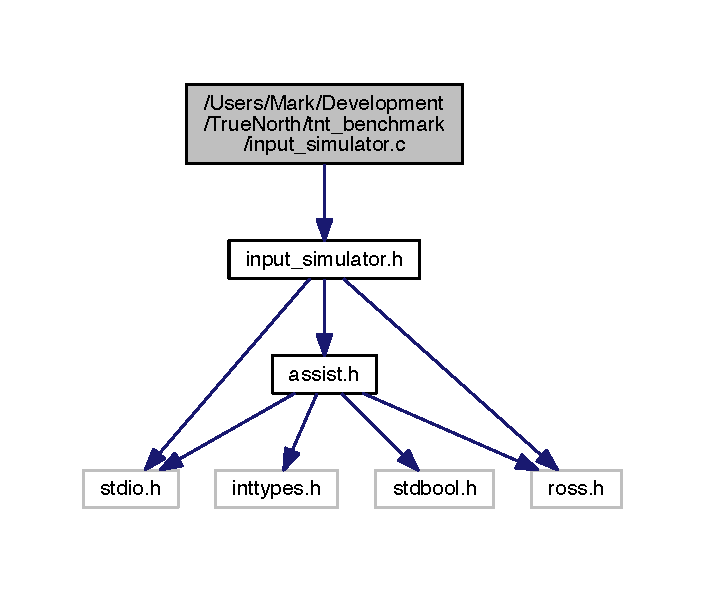
\includegraphics[width=340pt]{input__simulator_8c__incl}
\end{center}
\end{figure}
\subsection*{Functions}
\begin{DoxyCompactItemize}
\item 
bool \hyperlink{input__simulator_8c_a7ffa6df128d9c249ace6677ae62d1723}{uniform\+Gen} (void $\ast$spike\+Gen, tw\+\_\+lp $\ast$lp)
\end{DoxyCompactItemize}


\subsection{Function Documentation}
\hypertarget{input__simulator_8c_a7ffa6df128d9c249ace6677ae62d1723}{}\index{input\+\_\+simulator.\+c@{input\+\_\+simulator.\+c}!uniform\+Gen@{uniform\+Gen}}
\index{uniform\+Gen@{uniform\+Gen}!input\+\_\+simulator.\+c@{input\+\_\+simulator.\+c}}
\subsubsection[{uniform\+Gen}]{\setlength{\rightskip}{0pt plus 5cm}bool uniform\+Gen (
\begin{DoxyParamCaption}
\item[{void $\ast$}]{spike\+Gen, }
\item[{tw\+\_\+lp $\ast$}]{lp}
\end{DoxyParamCaption}
)}\label{input__simulator_8c_a7ffa6df128d9c249ace6677ae62d1723}


Definition at line \hyperlink{input__simulator_8c_source_l00010}{10} of file \hyperlink{input__simulator_8c_source}{input\+\_\+simulator.\+c}.



References \hyperlink{input__simulator_8h_source_l00050}{input\+Simulator\+State\+::random\+Rate}.


\begin{DoxyCode}
00010                                            \{
00011     \textcolor{keywordtype}{bool} willFire = \textcolor{keyword}{false};
00012 
00013     \hyperlink{structinput_simulator_state}{inputSimulatorState} * st = (\hyperlink{structinput_simulator_state}{inputSimulatorState} * ) spikeGen;
00014     tw\_rng\_stream *str = (tw\_rng\_stream *) lp->rng;
00015     \textcolor{keywordflow}{if}(tw\_rand\_unif(str) < st->\hyperlink{structinput_simulator_state_a1333eb5695ae83d1ffccf24b08bc6288}{randomRate})
00016         willFire = \textcolor{keyword}{true};
00017     \textcolor{keywordflow}{return} willFire;
00018 \}
\end{DoxyCode}

\hypertarget{input__simulator_8c_source}{}\section{/\+Users/\+Mark/\+Development/\+True\+North/tnt\+\_\+benchmark/input\+\_\+simulator.c}

\begin{DoxyCode}
00001 \textcolor{comment}{//}
00002 \textcolor{comment}{//  input\_simulator.c}
00003 \textcolor{comment}{//  ROSS\_TOP}
00004 \textcolor{comment}{//}
00005 \textcolor{comment}{//  Created by Mark Plagge on 6/18/15.}
00006 \textcolor{comment}{//}
00007 \textcolor{comment}{//}
00008 
00009 \textcolor{preprocessor}{#}\textcolor{preprocessor}{include} \hyperlink{input__simulator_8h}{"input\_simulator.h"}
\hypertarget{input__simulator_8c_source_l00010}{}\hyperlink{input__simulator_8h_ad6244e86a3542f8d3c64766e7e7c6746}{00010} \textcolor{keywordtype}{bool} \hyperlink{input__simulator_8h_ad6244e86a3542f8d3c64766e7e7c6746}{uniformGen}(\textcolor{keywordtype}{void} *spikeGen, tw\_lp *lp) \{
00011     \textcolor{keywordtype}{bool} willFire = \textcolor{keyword}{false};
00012 
00013     inputSimulatorState * st = (inputSimulatorState * ) spikeGen;
00014     tw\_rng\_stream *str = (tw\_rng\_stream *) lp->rng;
00015     \textcolor{keywordflow}{if}(tw\_rand\_unif(str) < st->randomRate)
00016         willFire = \textcolor{keyword}{true};
00017     \textcolor{keywordflow}{return} willFire;
00018 \}
\end{DoxyCode}

\hypertarget{input__simulator_8h}{}\section{/\+Users/\+Mark/\+Development/\+True\+North/tnt\+\_\+benchmark/input\+\_\+simulator.h File Reference}
\label{input__simulator_8h}\index{/\+Users/\+Mark/\+Development/\+True\+North/tnt\+\_\+benchmark/input\+\_\+simulator.\+h@{/\+Users/\+Mark/\+Development/\+True\+North/tnt\+\_\+benchmark/input\+\_\+simulator.\+h}}
{\ttfamily \#include $<$stdio.\+h$>$}\\*
{\ttfamily \#include \char`\"{}assist.\+h\char`\"{}}\\*
{\ttfamily \#include \char`\"{}ross.\+h\char`\"{}}\\*
Include dependency graph for input\+\_\+simulator.\+h\+:\nopagebreak
\begin{figure}[H]
\begin{center}
\leavevmode
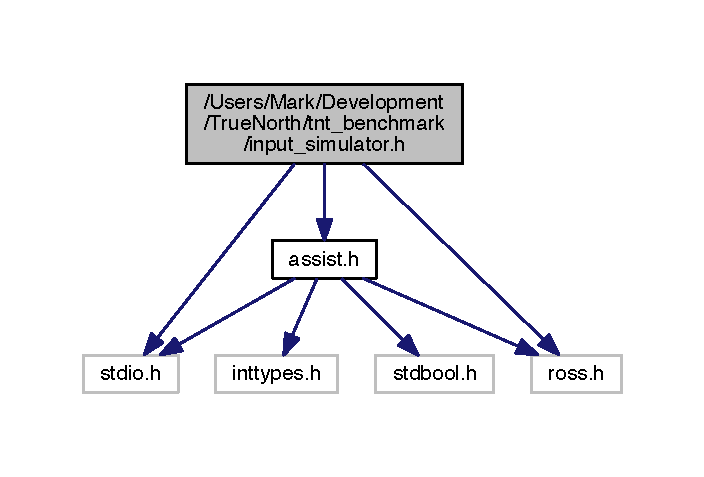
\includegraphics[width=338pt]{input__simulator_8h__incl}
\end{center}
\end{figure}
This graph shows which files directly or indirectly include this file\+:\nopagebreak
\begin{figure}[H]
\begin{center}
\leavevmode
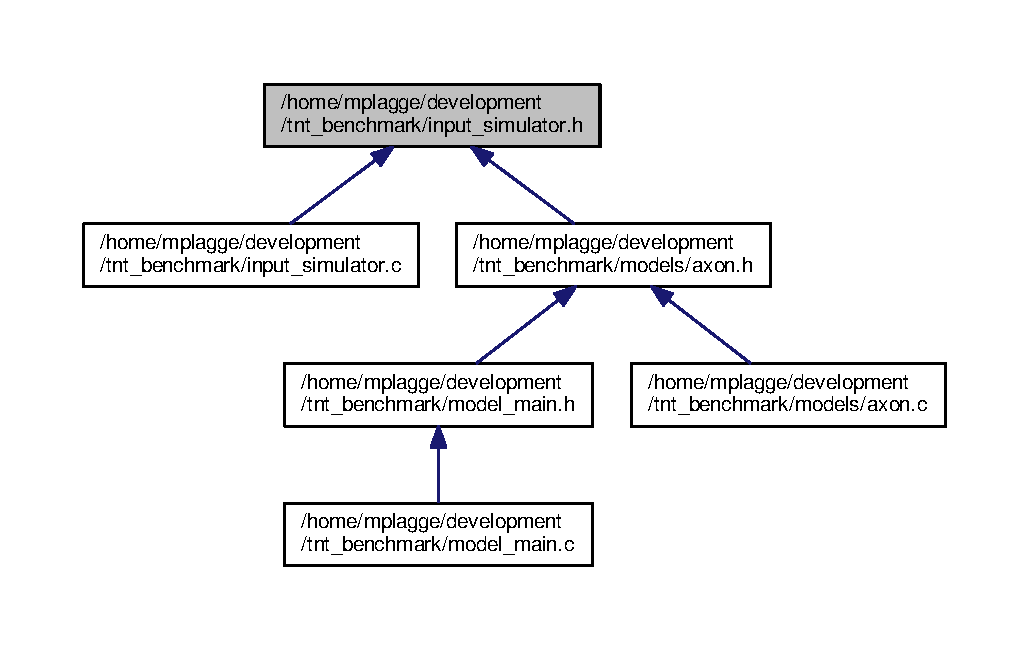
\includegraphics[width=350pt]{input__simulator_8h__dep__incl}
\end{center}
\end{figure}
\subsection*{Data Structures}
\begin{DoxyCompactItemize}
\item 
struct \hyperlink{structrandom_spikes}{random\+Spikes}
\begin{DoxyCompactList}\small\item\em Struct that genreates spikes randomly. \end{DoxyCompactList}\item 
struct \hyperlink{structselected_spikes}{selected\+Spikes}
\item 
struct \hyperlink{structinput_simulator_state}{input\+Simulator\+State}
\begin{DoxyCompactList}\small\item\em Struct that manages the spike generator. \end{DoxyCompactList}\end{DoxyCompactItemize}
\subsection*{Typedefs}
\begin{DoxyCompactItemize}
\item 
typedef bool($\ast$ \hyperlink{input__simulator_8h_aa47e87d309aab7727810011578bae86e}{spike\+Gen\+Del}) (void $\ast$spike\+Gen, tw\+\_\+lp $\ast$lp)
\begin{DoxyCompactList}\small\item\em Spike\+Generator Function Pointer. \end{DoxyCompactList}\end{DoxyCompactItemize}
\subsection*{Enumerations}
\begin{DoxyCompactItemize}
\item 
enum \hyperlink{input__simulator_8h_aa0d25534cd73156287b1136dd89c0215}{selected\+Random} \{ \hyperlink{input__simulator_8h_aa0d25534cd73156287b1136dd89c0215a4b3574e75cec43aa4dd3a0fd7940c632}{U\+N\+F}, 
\hyperlink{input__simulator_8h_aa0d25534cd73156287b1136dd89c0215ae003ec1158e3a4e295616ced12af154e}{N\+O\+R\+M}, 
\hyperlink{input__simulator_8h_aa0d25534cd73156287b1136dd89c0215a1697a91b22c2369eb2ba427c2d193329}{S\+E\+L\+E\+C\+T}
 \}
\end{DoxyCompactItemize}
\subsection*{Functions}
\begin{DoxyCompactItemize}
\item 
bool \hyperlink{input__simulator_8h_ad6244e86a3542f8d3c64766e7e7c6746}{uniform\+Gen} (void $\ast$gen\+\_\+state, tw\+\_\+lp $\ast$lp)
\item 
bool \hyperlink{input__simulator_8h_a7a9db804782d8a0c810fa90ae9c2dd05}{norm\+Gen} (void $\ast$gen\+\_\+state, tw\+\_\+lp $\ast$lp)
\item 
bool \hyperlink{input__simulator_8h_a7859f15c9115868c5c0ed88c43756482}{selected\+Gen} (void $\ast$spike\+Gen, tw\+\_\+lp $\ast$lp)
\end{DoxyCompactItemize}


\subsection{Typedef Documentation}
\hypertarget{input__simulator_8h_aa47e87d309aab7727810011578bae86e}{}\index{input\+\_\+simulator.\+h@{input\+\_\+simulator.\+h}!spike\+Gen\+Del@{spike\+Gen\+Del}}
\index{spike\+Gen\+Del@{spike\+Gen\+Del}!input\+\_\+simulator.\+h@{input\+\_\+simulator.\+h}}
\subsubsection[{spike\+Gen\+Del}]{\setlength{\rightskip}{0pt plus 5cm}typedef bool($\ast$ spike\+Gen\+Del) (void $\ast$spike\+Gen, tw\+\_\+lp $\ast$lp)}\label{input__simulator_8h_aa47e87d309aab7727810011578bae86e}


Spike\+Generator Function Pointer. 

Chooses the spike method function. 

Definition at line \hyperlink{input__simulator_8h_source_l00022}{22} of file \hyperlink{input__simulator_8h_source}{input\+\_\+simulator.\+h}.



\subsection{Enumeration Type Documentation}
\hypertarget{input__simulator_8h_aa0d25534cd73156287b1136dd89c0215}{}\index{input\+\_\+simulator.\+h@{input\+\_\+simulator.\+h}!selected\+Random@{selected\+Random}}
\index{selected\+Random@{selected\+Random}!input\+\_\+simulator.\+h@{input\+\_\+simulator.\+h}}
\subsubsection[{selected\+Random}]{\setlength{\rightskip}{0pt plus 5cm}enum {\bf selected\+Random}}\label{input__simulator_8h_aa0d25534cd73156287b1136dd89c0215}
\begin{Desc}
\item[Enumerator]\par
\begin{description}
\index{U\+N\+F@{U\+N\+F}!input\+\_\+simulator.\+h@{input\+\_\+simulator.\+h}}\index{input\+\_\+simulator.\+h@{input\+\_\+simulator.\+h}!U\+N\+F@{U\+N\+F}}\item[{\em 
\hypertarget{input__simulator_8h_aa0d25534cd73156287b1136dd89c0215a4b3574e75cec43aa4dd3a0fd7940c632}{}U\+N\+F\label{input__simulator_8h_aa0d25534cd73156287b1136dd89c0215a4b3574e75cec43aa4dd3a0fd7940c632}
}]\index{N\+O\+R\+M@{N\+O\+R\+M}!input\+\_\+simulator.\+h@{input\+\_\+simulator.\+h}}\index{input\+\_\+simulator.\+h@{input\+\_\+simulator.\+h}!N\+O\+R\+M@{N\+O\+R\+M}}\item[{\em 
\hypertarget{input__simulator_8h_aa0d25534cd73156287b1136dd89c0215ae003ec1158e3a4e295616ced12af154e}{}N\+O\+R\+M\label{input__simulator_8h_aa0d25534cd73156287b1136dd89c0215ae003ec1158e3a4e295616ced12af154e}
}]\index{S\+E\+L\+E\+C\+T@{S\+E\+L\+E\+C\+T}!input\+\_\+simulator.\+h@{input\+\_\+simulator.\+h}}\index{input\+\_\+simulator.\+h@{input\+\_\+simulator.\+h}!S\+E\+L\+E\+C\+T@{S\+E\+L\+E\+C\+T}}\item[{\em 
\hypertarget{input__simulator_8h_aa0d25534cd73156287b1136dd89c0215a1697a91b22c2369eb2ba427c2d193329}{}S\+E\+L\+E\+C\+T\label{input__simulator_8h_aa0d25534cd73156287b1136dd89c0215a1697a91b22c2369eb2ba427c2d193329}
}]\end{description}
\end{Desc}


Definition at line \hyperlink{input__simulator_8h_source_l00016}{16} of file \hyperlink{input__simulator_8h_source}{input\+\_\+simulator.\+h}.


\begin{DoxyCode}
00016                             \{
00017     \hyperlink{input__simulator_8h_aa0d25534cd73156287b1136dd89c0215a4b3574e75cec43aa4dd3a0fd7940c632}{UNF},
00018     \hyperlink{input__simulator_8h_aa0d25534cd73156287b1136dd89c0215ae003ec1158e3a4e295616ced12af154e}{NORM},
00019     \hyperlink{input__simulator_8h_aa0d25534cd73156287b1136dd89c0215a1697a91b22c2369eb2ba427c2d193329}{SELECT}
00020 \}\hyperlink{input__simulator_8h_aa0d25534cd73156287b1136dd89c0215}{selectedRandom};
\end{DoxyCode}


\subsection{Function Documentation}
\hypertarget{input__simulator_8h_a7a9db804782d8a0c810fa90ae9c2dd05}{}\index{input\+\_\+simulator.\+h@{input\+\_\+simulator.\+h}!norm\+Gen@{norm\+Gen}}
\index{norm\+Gen@{norm\+Gen}!input\+\_\+simulator.\+h@{input\+\_\+simulator.\+h}}
\subsubsection[{norm\+Gen}]{\setlength{\rightskip}{0pt plus 5cm}bool norm\+Gen (
\begin{DoxyParamCaption}
\item[{void $\ast$}]{gen\+\_\+state, }
\item[{tw\+\_\+lp $\ast$}]{lp}
\end{DoxyParamCaption}
)}\label{input__simulator_8h_a7a9db804782d8a0c810fa90ae9c2dd05}
\hypertarget{input__simulator_8h_a7859f15c9115868c5c0ed88c43756482}{}\index{input\+\_\+simulator.\+h@{input\+\_\+simulator.\+h}!selected\+Gen@{selected\+Gen}}
\index{selected\+Gen@{selected\+Gen}!input\+\_\+simulator.\+h@{input\+\_\+simulator.\+h}}
\subsubsection[{selected\+Gen}]{\setlength{\rightskip}{0pt plus 5cm}bool selected\+Gen (
\begin{DoxyParamCaption}
\item[{void $\ast$}]{spike\+Gen, }
\item[{tw\+\_\+lp $\ast$}]{lp}
\end{DoxyParamCaption}
)}\label{input__simulator_8h_a7859f15c9115868c5c0ed88c43756482}
\hypertarget{input__simulator_8h_ad6244e86a3542f8d3c64766e7e7c6746}{}\index{input\+\_\+simulator.\+h@{input\+\_\+simulator.\+h}!uniform\+Gen@{uniform\+Gen}}
\index{uniform\+Gen@{uniform\+Gen}!input\+\_\+simulator.\+h@{input\+\_\+simulator.\+h}}
\subsubsection[{uniform\+Gen}]{\setlength{\rightskip}{0pt plus 5cm}bool uniform\+Gen (
\begin{DoxyParamCaption}
\item[{void $\ast$}]{gen\+\_\+state, }
\item[{tw\+\_\+lp $\ast$}]{lp}
\end{DoxyParamCaption}
)}\label{input__simulator_8h_ad6244e86a3542f8d3c64766e7e7c6746}


Definition at line \hyperlink{input__simulator_8c_source_l00010}{10} of file \hyperlink{input__simulator_8c_source}{input\+\_\+simulator.\+c}.


\begin{DoxyCode}
00010                                            \{
00011     \textcolor{keywordtype}{bool} willFire = \textcolor{keyword}{false};
00012 
00013     \hyperlink{structinput_simulator_state}{inputSimulatorState} * st = (\hyperlink{structinput_simulator_state}{inputSimulatorState} * ) spikeGen;
00014     tw\_rng\_stream *str = (tw\_rng\_stream *) lp->rng;
00015     \textcolor{keywordflow}{if}(tw\_rand\_unif(str) < st->\hyperlink{structinput_simulator_state_a1333eb5695ae83d1ffccf24b08bc6288}{randomRate})
00016         willFire = \textcolor{keyword}{true};
00017     \textcolor{keywordflow}{return} willFire;
00018 \}\end{DoxyCode}

\hypertarget{input__simulator_8h_source}{}\section{/home/mplagge/development/tnt\+\_\+benchmark/input\+\_\+simulator.h}

\begin{DoxyCode}
00001 \textcolor{comment}{//}
00002 \textcolor{comment}{//  input\_simulator.h}
00003 \textcolor{comment}{//  ROSS\_TOP}
00004 \textcolor{comment}{//}
00005 \textcolor{comment}{//  Created by Mark Plagge on 6/18/15.}
00006 \textcolor{comment}{//}
00007 \textcolor{comment}{//}
00008 
00009 \textcolor{preprocessor}{#ifndef \_\_ROSS\_TOP\_\_input\_simulator\_\_}
00010 \textcolor{preprocessor}{#define \_\_ROSS\_TOP\_\_input\_simulator\_\_}
00011 
00012 \textcolor{preprocessor}{#include <stdio.h>}
00013 \textcolor{preprocessor}{#include "\hyperlink{assist_8h}{assist.h}"}
00014 \textcolor{preprocessor}{#include "ross.h"}
00015 
\hypertarget{input__simulator_8h_source_l00016}{}\hyperlink{input__simulator_8h_aa0d25534cd73156287b1136dd89c0215}{00016} \textcolor{keyword}{typedef} \textcolor{keyword}{enum} SelectedRandom \{
\hypertarget{input__simulator_8h_source_l00017}{}\hyperlink{input__simulator_8h_aa0d25534cd73156287b1136dd89c0215a4b3574e75cec43aa4dd3a0fd7940c632}{00017}     \hyperlink{input__simulator_8h_aa0d25534cd73156287b1136dd89c0215a4b3574e75cec43aa4dd3a0fd7940c632}{UNF},
\hypertarget{input__simulator_8h_source_l00018}{}\hyperlink{input__simulator_8h_aa0d25534cd73156287b1136dd89c0215ae003ec1158e3a4e295616ced12af154e}{00018}     \hyperlink{input__simulator_8h_aa0d25534cd73156287b1136dd89c0215ae003ec1158e3a4e295616ced12af154e}{NORM},
\hypertarget{input__simulator_8h_source_l00019}{}\hyperlink{input__simulator_8h_aa0d25534cd73156287b1136dd89c0215a1697a91b22c2369eb2ba427c2d193329}{00019}     \hyperlink{input__simulator_8h_aa0d25534cd73156287b1136dd89c0215a1697a91b22c2369eb2ba427c2d193329}{SELECT}
00020 \}\hyperlink{input__simulator_8h_aa0d25534cd73156287b1136dd89c0215}{selectedRandom};
\hypertarget{input__simulator_8h_source_l00022}{}\hyperlink{input__simulator_8h_aa47e87d309aab7727810011578bae86e}{00022} \textcolor{keyword}{typedef} bool (*\hyperlink{input__simulator_8h_aa47e87d309aab7727810011578bae86e}{spikeGenDel})(\textcolor{keywordtype}{void} *spikeGen, tw\_lp *lp);
00023 \textcolor{keywordtype}{bool} \hyperlink{input__simulator_8h_ad6244e86a3542f8d3c64766e7e7c6746}{uniformGen}(\textcolor{keywordtype}{void} *gen\_state, tw\_lp *lp);
00024 \textcolor{keywordtype}{bool} \hyperlink{input__simulator_8h_a7a9db804782d8a0c810fa90ae9c2dd05}{normGen}(\textcolor{keywordtype}{void} *gen\_state, tw\_lp *lp);
00025 \textcolor{keywordtype}{bool} \hyperlink{input__simulator_8h_a7859f15c9115868c5c0ed88c43756482}{selectedGen}(\textcolor{keywordtype}{void} *spikeGen, tw\_lp *lp);
00026 
00027 
\hypertarget{input__simulator_8h_source_l00029}{}\hyperlink{structrandom_spikes}{00029} \textcolor{keyword}{typedef} \textcolor{keyword}{struct }RandomSpikes \{
\hypertarget{input__simulator_8h_source_l00030}{}\hyperlink{structrandom_spikes_a1333eb5695ae83d1ffccf24b08bc6288}{00030}     \textcolor{keywordtype}{float} \hyperlink{structrandom_spikes_a1333eb5695ae83d1ffccf24b08bc6288}{randomRate}; 
\hypertarget{input__simulator_8h_source_l00031}{}\hyperlink{structrandom_spikes_a18766f12fc4212349fb61b221f83b779}{00031}     \hyperlink{input__simulator_8h_aa0d25534cd73156287b1136dd89c0215}{selectedRandom} \hyperlink{structrandom_spikes_a18766f12fc4212349fb61b221f83b779}{randMethod}; 
\hypertarget{input__simulator_8h_source_l00032}{}\hyperlink{structrandom_spikes_a0eb8199754a403ccc8eac256f9193a02}{00032}     \textcolor{keywordtype}{float} \hyperlink{structrandom_spikes_a0eb8199754a403ccc8eac256f9193a02}{rndFctVal}; 
00033 \}\hyperlink{structrandom_spikes}{randomSpikes};
00034 
\hypertarget{input__simulator_8h_source_l00035}{}\hyperlink{structselected_spikes}{00035} \textcolor{keyword}{typedef} \textcolor{keyword}{struct }SelectedSpikes \{
\hypertarget{input__simulator_8h_source_l00036}{}\hyperlink{structselected_spikes_a666eb9ad96121cf3e4ce134e1a4c12c0}{00036}     \textcolor{keywordtype}{int} * \hyperlink{structselected_spikes_a666eb9ad96121cf3e4ce134e1a4c12c0}{outputMesh}; 
\hypertarget{input__simulator_8h_source_l00037}{}\hyperlink{structselected_spikes_a97727a3be0dbd5813f860c99733048a8}{00037}     \textcolor{keywordtype}{int} \hyperlink{structselected_spikes_a97727a3be0dbd5813f860c99733048a8}{outputMeshLengh}; 
00038 \}\hyperlink{structselected_spikes}{selectedSpikes};
00039 
\hypertarget{input__simulator_8h_source_l00042}{}\hyperlink{structinput_simulator_state}{00042} \textcolor{keyword}{typedef} \textcolor{keyword}{struct }InputSimulator \{
\hypertarget{input__simulator_8h_source_l00043}{}\hyperlink{structinput_simulator_state_af892db49cef1c5e5d95010561e549678}{00043}     \textcolor{keywordtype}{int} \hyperlink{structinput_simulator_state_af892db49cef1c5e5d95010561e549678}{outbound}; 
\hypertarget{input__simulator_8h_source_l00044}{}\hyperlink{structinput_simulator_state_a569dc67b8984bb0a3616bf17f9763ebb}{00044}     tw\_lpid *\hyperlink{structinput_simulator_state_a569dc67b8984bb0a3616bf17f9763ebb}{connectedSynapses}; 
\hypertarget{input__simulator_8h_source_l00045}{}\hyperlink{structinput_simulator_state_ae40f21a48f3157bcad074f424046ed2c}{00045}     \hyperlink{input__simulator_8h_aa47e87d309aab7727810011578bae86e}{spikeGenDel} \hyperlink{structinput_simulator_state_ae40f21a48f3157bcad074f424046ed2c}{spikeGen};
00046         \textcolor{comment}{//selectedSpikes  selSpikes;}
00047         \textcolor{comment}{//randomSpikes  rndSpikes;}
\hypertarget{input__simulator_8h_source_l00048}{}\hyperlink{structinput_simulator_state_a666eb9ad96121cf3e4ce134e1a4c12c0}{00048}     \textcolor{keywordtype}{int} * \hyperlink{structinput_simulator_state_a666eb9ad96121cf3e4ce134e1a4c12c0}{outputMesh}; 
\hypertarget{input__simulator_8h_source_l00049}{}\hyperlink{structinput_simulator_state_a97727a3be0dbd5813f860c99733048a8}{00049}     \textcolor{keywordtype}{int} \hyperlink{structinput_simulator_state_a97727a3be0dbd5813f860c99733048a8}{outputMeshLengh}; 
\hypertarget{input__simulator_8h_source_l00050}{}\hyperlink{structinput_simulator_state_a1333eb5695ae83d1ffccf24b08bc6288}{00050}     \textcolor{keywordtype}{float} \hyperlink{structinput_simulator_state_a1333eb5695ae83d1ffccf24b08bc6288}{randomRate}; 
\hypertarget{input__simulator_8h_source_l00051}{}\hyperlink{structinput_simulator_state_a18766f12fc4212349fb61b221f83b779}{00051}     \hyperlink{input__simulator_8h_aa0d25534cd73156287b1136dd89c0215}{selectedRandom} \hyperlink{structinput_simulator_state_a18766f12fc4212349fb61b221f83b779}{randMethod}; 
\hypertarget{input__simulator_8h_source_l00052}{}\hyperlink{structinput_simulator_state_a0eb8199754a403ccc8eac256f9193a02}{00052}     \textcolor{keywordtype}{float} \hyperlink{structinput_simulator_state_a0eb8199754a403ccc8eac256f9193a02}{rndFctVal}; 
\hypertarget{input__simulator_8h_source_l00053}{}\hyperlink{structinput_simulator_state_accc0c3f890194cda401a16f5f54e43cb}{00053}     \textcolor{keywordtype}{int} \hyperlink{structinput_simulator_state_accc0c3f890194cda401a16f5f54e43cb}{currentOut}; 
00055 \}\hyperlink{structinput_simulator_state}{inputSimulatorState};
00056 \textcolor{preprocessor}{#endif }\textcolor{comment}{/* defined(\_\_ROSS\_TOP\_\_input\_simulator\_\_) */}\textcolor{preprocessor}{}
\end{DoxyCode}

\hypertarget{mapping_8c}{}\section{/home/mplagge/development/tnt\+\_\+benchmark/mapping.c File Reference}
\label{mapping_8c}\index{/home/mplagge/development/tnt\+\_\+benchmark/mapping.\+c@{/home/mplagge/development/tnt\+\_\+benchmark/mapping.\+c}}
{\ttfamily \#include \char`\"{}mapping.\+h\char`\"{}}\\*
Include dependency graph for mapping.\+c\+:\nopagebreak
\begin{figure}[H]
\begin{center}
\leavevmode
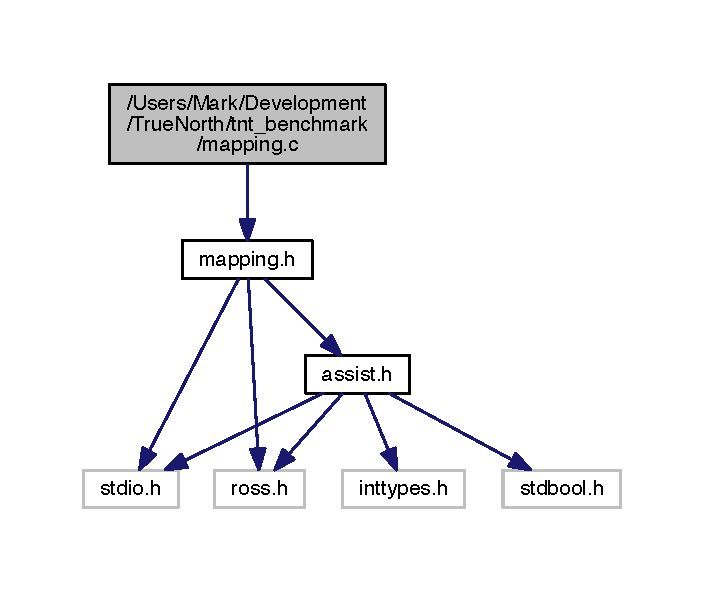
\includegraphics[width=340pt]{mapping_8c__incl}
\end{center}
\end{figure}

\hypertarget{mapping_8c_source}{}\section{/\+Users/\+Mark/\+Development/\+True\+North/tnt\+\_\+benchmark/mapping.c}

\begin{DoxyCode}
00001 \textcolor{comment}{//}
00002 \textcolor{comment}{//  mapping.c}
00003 \textcolor{comment}{//  ROSS\_TOP}
00004 \textcolor{comment}{//}
00005 \textcolor{comment}{//  Created by Mark Plagge on 6/18/15.}
00006 \textcolor{comment}{//}
00007 \textcolor{comment}{//}
00008 
00009 \textcolor{preprocessor}{#}\textcolor{preprocessor}{include} \hyperlink{mapping_8h}{"mapping.h"}
\end{DoxyCode}

\hypertarget{mapping_8h}{}\section{/home/mplagge/development/tnt\+\_\+benchmark/mapping.h File Reference}
\label{mapping_8h}\index{/home/mplagge/development/tnt\+\_\+benchmark/mapping.\+h@{/home/mplagge/development/tnt\+\_\+benchmark/mapping.\+h}}
{\ttfamily \#include $<$stdio.\+h$>$}\\*
{\ttfamily \#include \char`\"{}ross.\+h\char`\"{}}\\*
{\ttfamily \#include \char`\"{}assist.\+h\char`\"{}}\\*
Include dependency graph for mapping.\+h\+:\nopagebreak
\begin{figure}[H]
\begin{center}
\leavevmode
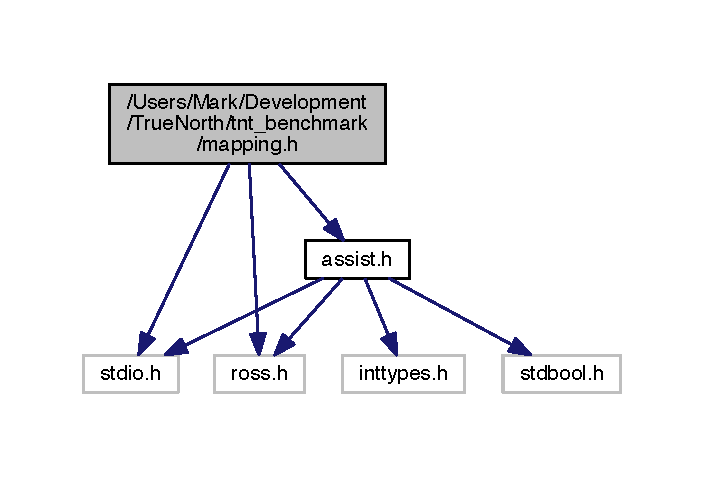
\includegraphics[width=340pt]{mapping_8h__incl}
\end{center}
\end{figure}
This graph shows which files directly or indirectly include this file\+:\nopagebreak
\begin{figure}[H]
\begin{center}
\leavevmode
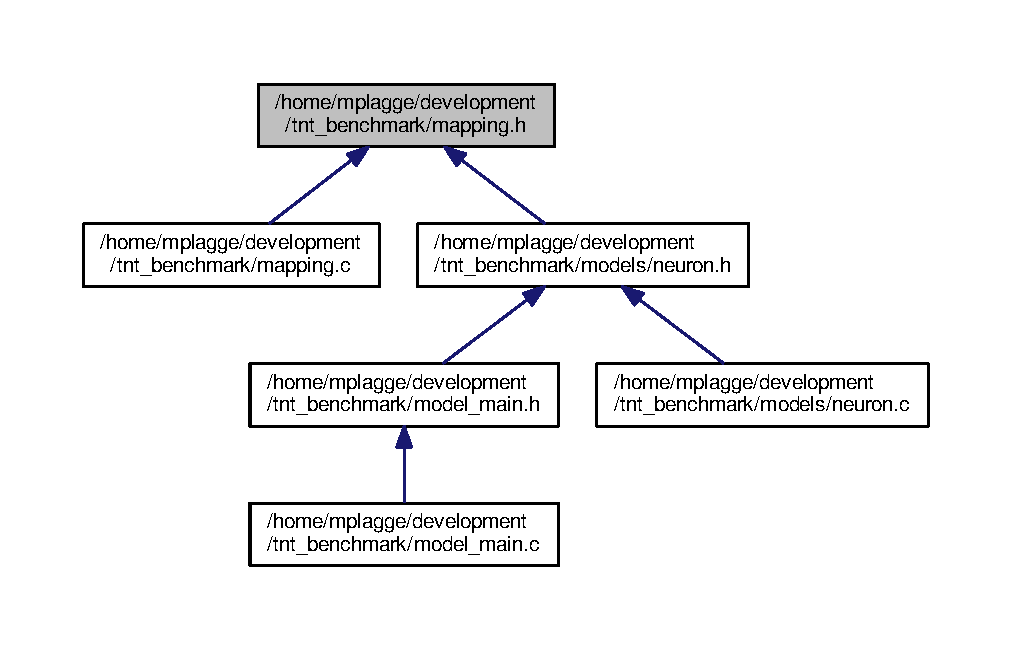
\includegraphics[width=350pt]{mapping_8h__dep__incl}
\end{center}
\end{figure}
\subsection*{Functions}
\begin{DoxyCompactItemize}
\item 
tw\+\_\+peid \hyperlink{mapping_8h_ab67eefe1d34d874bcd5f8cfa854e7fc7}{lp\+To\+Pe\+Map} (tw\+\_\+peid gid)
\begin{DoxyCompactList}\small\item\em Custom Mapping -\/ given a L\+P G\+I\+D return a P\+E. \end{DoxyCompactList}\item 
void \hyperlink{mapping_8h_af6a8846083f1bd8ca747136c3b5967d8}{mapping\+Setup} ()
\begin{DoxyCompactList}\small\item\em Setup mapping per P\+E. \end{DoxyCompactList}\item 
tw\+\_\+lp $\ast$ \hyperlink{mapping_8h_a65ae45764256c6f8a0552ec04a132fcf}{global\+To\+Local} (tw\+\_\+lpid gid)
\begin{DoxyCompactList}\small\item\em Given a global I\+D, return a L\+P. \end{DoxyCompactList}\end{DoxyCompactItemize}
\subsection*{Variables}
\begin{DoxyCompactItemize}
\item 
int \hyperlink{mapping_8h_a67e8e45768f76b984a60fcff2b7c51aa}{N\+E\+U\+R\+O\+N\+S\+\_\+\+I\+N\+\_\+\+C\+O\+R\+E}
\begin{DoxyCompactList}\small\item\em Number of neurons per core. \end{DoxyCompactList}\item 
int \hyperlink{mapping_8h_a076b99099b46431255982b2bb8ce06fb}{S\+Y\+N\+A\+P\+S\+E\+S\+\_\+\+I\+N\+\_\+\+C\+O\+R\+E}
\begin{DoxyCompactList}\small\item\em Number of synapses per core. \end{DoxyCompactList}\item 
int \hyperlink{mapping_8h_ad39b86a0b748731175572436f6672264}{C\+O\+R\+E\+\_\+\+S\+I\+Z\+E}
\begin{DoxyCompactList}\small\item\em C\+O\+R\+E\+\_\+\+S\+I\+Z\+E is equal to the number of axions $\ast$ number of aneurons + num neurons + num axions. \end{DoxyCompactList}\item 
int \hyperlink{mapping_8h_afe9ee9518533aa222adff4a27ff09281}{nlp\+\_\+per\+\_\+kp}
\item 
int \hyperlink{mapping_8h_a929a1afa1773005b4881bea7869fdb60}{nkp\+\_\+per\+\_\+pe}
\item 
int \hyperlink{mapping_8h_ae2910f7a5d9f53ae602e62bb0248edba}{C\+O\+R\+E\+\_\+\+L\+P\+\_\+\+O\+F\+F\+S\+E\+T}
\begin{DoxyCompactList}\small\item\em C\+O\+R\+E\+\_\+\+L\+P\+\_\+\+O\+F\+F\+S\+E\+T -\/ Manages the offset. \end{DoxyCompactList}\item 
int \hyperlink{mapping_8h_a1d3b60109ac1c91025d512707a3242a8}{C\+P\+E}
\end{DoxyCompactItemize}


\subsection{Function Documentation}
\hypertarget{mapping_8h_a65ae45764256c6f8a0552ec04a132fcf}{}\index{mapping.\+h@{mapping.\+h}!global\+To\+Local@{global\+To\+Local}}
\index{global\+To\+Local@{global\+To\+Local}!mapping.\+h@{mapping.\+h}}
\subsubsection[{global\+To\+Local}]{\setlength{\rightskip}{0pt plus 5cm}tw\+\_\+lp$\ast$ global\+To\+Local (
\begin{DoxyParamCaption}
\item[{tw\+\_\+lpid}]{gid}
\end{DoxyParamCaption}
)}\label{mapping_8h_a65ae45764256c6f8a0552ec04a132fcf}


Given a global I\+D, return a L\+P. 


\begin{DoxyParams}{Parameters}
{\em gid} & $<$\#gid description\#$>$\\
\hline
\end{DoxyParams}
\begin{DoxyReturn}{Returns}
$<$\#return value description\#$>$ 
\end{DoxyReturn}
\hypertarget{mapping_8h_ab67eefe1d34d874bcd5f8cfa854e7fc7}{}\index{mapping.\+h@{mapping.\+h}!lp\+To\+Pe\+Map@{lp\+To\+Pe\+Map}}
\index{lp\+To\+Pe\+Map@{lp\+To\+Pe\+Map}!mapping.\+h@{mapping.\+h}}
\subsubsection[{lp\+To\+Pe\+Map}]{\setlength{\rightskip}{0pt plus 5cm}tw\+\_\+peid lp\+To\+Pe\+Map (
\begin{DoxyParamCaption}
\item[{tw\+\_\+peid}]{gid}
\end{DoxyParamCaption}
)}\label{mapping_8h_ab67eefe1d34d874bcd5f8cfa854e7fc7}


Custom Mapping -\/ given a L\+P G\+I\+D return a P\+E. 


\begin{DoxyParams}{Parameters}
{\em gid} & $<$\#gid description\#$>$\\
\hline
\end{DoxyParams}
\begin{DoxyReturn}{Returns}
$<$\#return value description\#$>$ 
\end{DoxyReturn}
\hypertarget{mapping_8h_af6a8846083f1bd8ca747136c3b5967d8}{}\index{mapping.\+h@{mapping.\+h}!mapping\+Setup@{mapping\+Setup}}
\index{mapping\+Setup@{mapping\+Setup}!mapping.\+h@{mapping.\+h}}
\subsubsection[{mapping\+Setup}]{\setlength{\rightskip}{0pt plus 5cm}void mapping\+Setup (
\begin{DoxyParamCaption}
{}
\end{DoxyParamCaption}
)}\label{mapping_8h_af6a8846083f1bd8ca747136c3b5967d8}


Setup mapping per P\+E. 



\subsection{Variable Documentation}
\hypertarget{mapping_8h_ae2910f7a5d9f53ae602e62bb0248edba}{}\index{mapping.\+h@{mapping.\+h}!C\+O\+R\+E\+\_\+\+L\+P\+\_\+\+O\+F\+F\+S\+E\+T@{C\+O\+R\+E\+\_\+\+L\+P\+\_\+\+O\+F\+F\+S\+E\+T}}
\index{C\+O\+R\+E\+\_\+\+L\+P\+\_\+\+O\+F\+F\+S\+E\+T@{C\+O\+R\+E\+\_\+\+L\+P\+\_\+\+O\+F\+F\+S\+E\+T}!mapping.\+h@{mapping.\+h}}
\subsubsection[{C\+O\+R\+E\+\_\+\+L\+P\+\_\+\+O\+F\+F\+S\+E\+T}]{\setlength{\rightskip}{0pt plus 5cm}int C\+O\+R\+E\+\_\+\+L\+P\+\_\+\+O\+F\+F\+S\+E\+T}\label{mapping_8h_ae2910f7a5d9f53ae602e62bb0248edba}


C\+O\+R\+E\+\_\+\+L\+P\+\_\+\+O\+F\+F\+S\+E\+T -\/ Manages the offset. 

Calculated based on the size of a core, and the C\+P\+E vale, the number of P\+Es required to simulate a single core. For example, if core size is 128, and C\+P\+E is 2, then each P\+E will get 64 L\+Ps. T\+O\+D\+O\+: Add a synapse and neuron balancing function. 

Definition at line \hyperlink{mapping_8h_source_l00034}{34} of file \hyperlink{mapping_8h_source}{mapping.\+h}.

\hypertarget{mapping_8h_ad39b86a0b748731175572436f6672264}{}\index{mapping.\+h@{mapping.\+h}!C\+O\+R\+E\+\_\+\+S\+I\+Z\+E@{C\+O\+R\+E\+\_\+\+S\+I\+Z\+E}}
\index{C\+O\+R\+E\+\_\+\+S\+I\+Z\+E@{C\+O\+R\+E\+\_\+\+S\+I\+Z\+E}!mapping.\+h@{mapping.\+h}}
\subsubsection[{C\+O\+R\+E\+\_\+\+S\+I\+Z\+E}]{\setlength{\rightskip}{0pt plus 5cm}int C\+O\+R\+E\+\_\+\+S\+I\+Z\+E}\label{mapping_8h_ad39b86a0b748731175572436f6672264}


C\+O\+R\+E\+\_\+\+S\+I\+Z\+E is equal to the number of axions $\ast$ number of aneurons + num neurons + num axions. 



Definition at line \hyperlink{model__main_8h_source_l00063}{63} of file \hyperlink{model__main_8h_source}{model\+\_\+main.\+h}.

\hypertarget{mapping_8h_a1d3b60109ac1c91025d512707a3242a8}{}\index{mapping.\+h@{mapping.\+h}!C\+P\+E@{C\+P\+E}}
\index{C\+P\+E@{C\+P\+E}!mapping.\+h@{mapping.\+h}}
\subsubsection[{C\+P\+E}]{\setlength{\rightskip}{0pt plus 5cm}int C\+P\+E}\label{mapping_8h_a1d3b60109ac1c91025d512707a3242a8}
\hypertarget{mapping_8h_a67e8e45768f76b984a60fcff2b7c51aa}{}\index{mapping.\+h@{mapping.\+h}!N\+E\+U\+R\+O\+N\+S\+\_\+\+I\+N\+\_\+\+C\+O\+R\+E@{N\+E\+U\+R\+O\+N\+S\+\_\+\+I\+N\+\_\+\+C\+O\+R\+E}}
\index{N\+E\+U\+R\+O\+N\+S\+\_\+\+I\+N\+\_\+\+C\+O\+R\+E@{N\+E\+U\+R\+O\+N\+S\+\_\+\+I\+N\+\_\+\+C\+O\+R\+E}!mapping.\+h@{mapping.\+h}}
\subsubsection[{N\+E\+U\+R\+O\+N\+S\+\_\+\+I\+N\+\_\+\+C\+O\+R\+E}]{\setlength{\rightskip}{0pt plus 5cm}int N\+E\+U\+R\+O\+N\+S\+\_\+\+I\+N\+\_\+\+C\+O\+R\+E}\label{mapping_8h_a67e8e45768f76b984a60fcff2b7c51aa}


Number of neurons per core. 

/name Sim\+Params 

Definition at line \hyperlink{model__main_8h_source_l00024}{24} of file \hyperlink{model__main_8h_source}{model\+\_\+main.\+h}.

\hypertarget{mapping_8h_a929a1afa1773005b4881bea7869fdb60}{}\index{mapping.\+h@{mapping.\+h}!nkp\+\_\+per\+\_\+pe@{nkp\+\_\+per\+\_\+pe}}
\index{nkp\+\_\+per\+\_\+pe@{nkp\+\_\+per\+\_\+pe}!mapping.\+h@{mapping.\+h}}
\subsubsection[{nkp\+\_\+per\+\_\+pe}]{\setlength{\rightskip}{0pt plus 5cm}int nkp\+\_\+per\+\_\+pe}\label{mapping_8h_a929a1afa1773005b4881bea7869fdb60}
\hypertarget{mapping_8h_afe9ee9518533aa222adff4a27ff09281}{}\index{mapping.\+h@{mapping.\+h}!nlp\+\_\+per\+\_\+kp@{nlp\+\_\+per\+\_\+kp}}
\index{nlp\+\_\+per\+\_\+kp@{nlp\+\_\+per\+\_\+kp}!mapping.\+h@{mapping.\+h}}
\subsubsection[{nlp\+\_\+per\+\_\+kp}]{\setlength{\rightskip}{0pt plus 5cm}int nlp\+\_\+per\+\_\+kp}\label{mapping_8h_afe9ee9518533aa222adff4a27ff09281}
\hypertarget{mapping_8h_a076b99099b46431255982b2bb8ce06fb}{}\index{mapping.\+h@{mapping.\+h}!S\+Y\+N\+A\+P\+S\+E\+S\+\_\+\+I\+N\+\_\+\+C\+O\+R\+E@{S\+Y\+N\+A\+P\+S\+E\+S\+\_\+\+I\+N\+\_\+\+C\+O\+R\+E}}
\index{S\+Y\+N\+A\+P\+S\+E\+S\+\_\+\+I\+N\+\_\+\+C\+O\+R\+E@{S\+Y\+N\+A\+P\+S\+E\+S\+\_\+\+I\+N\+\_\+\+C\+O\+R\+E}!mapping.\+h@{mapping.\+h}}
\subsubsection[{S\+Y\+N\+A\+P\+S\+E\+S\+\_\+\+I\+N\+\_\+\+C\+O\+R\+E}]{\setlength{\rightskip}{0pt plus 5cm}int S\+Y\+N\+A\+P\+S\+E\+S\+\_\+\+I\+N\+\_\+\+C\+O\+R\+E}\label{mapping_8h_a076b99099b46431255982b2bb8ce06fb}


Number of synapses per core. 

Number of synapses per core.

Calculated value, needs to be neurons $\ast$ axons 

Definition at line \hyperlink{model__main_8h_source_l00026}{26} of file \hyperlink{model__main_8h_source}{model\+\_\+main.\+h}.


\hypertarget{mapping_8h_source}{}\section{/\+Users/\+Mark/\+Development/\+True\+North/tnt\+\_\+benchmark/mapping.h}

\begin{DoxyCode}
00001 \textcolor{comment}{//}
00002 \textcolor{comment}{//  mapping.h}
00003 \textcolor{comment}{//  ROSS\_TOP}
00004 \textcolor{comment}{//}
00005 \textcolor{comment}{//  Created by Mark Plagge on 6/18/15.}
00006 \textcolor{comment}{//}
00007 \textcolor{comment}{//}
00008 
00009 \textcolor{preprocessor}{#}\textcolor{preprocessor}{ifndef} \textcolor{preprocessor}{\_\_ROSS\_TOP\_\_mapping\_\_}
00010 \textcolor{preprocessor}{#}\textcolor{preprocessor}{define} \textcolor{preprocessor}{\_\_ROSS\_TOP\_\_mapping\_\_}
00011 
00012 \textcolor{preprocessor}{#}\textcolor{preprocessor}{include} \textcolor{preprocessor}{<}\textcolor{preprocessor}{stdio}\textcolor{preprocessor}{.}\textcolor{preprocessor}{h}\textcolor{preprocessor}{>}
00013 \textcolor{preprocessor}{#}\textcolor{preprocessor}{include} \textcolor{preprocessor}{"ross.h"}
00014 \textcolor{preprocessor}{#}\textcolor{preprocessor}{include} \hyperlink{assist_8h}{"assist.h"}
00015 
00016 \textcolor{preprocessor}{#}\textcolor{preprocessor}{endif} \textcolor{comment}{/* defined(\_\_ROSS\_TOP\_\_mapping\_\_) */}
\end{DoxyCode}

\hypertarget{model__main_8c}{}\section{/\+Users/\+Mark/\+Development/\+True\+North/tnt\+\_\+benchmark/model\+\_\+main.c File Reference}
\label{model__main_8c}\index{/\+Users/\+Mark/\+Development/\+True\+North/tnt\+\_\+benchmark/model\+\_\+main.\+c@{/\+Users/\+Mark/\+Development/\+True\+North/tnt\+\_\+benchmark/model\+\_\+main.\+c}}
{\ttfamily \#include \char`\"{}model\+\_\+main.\+h\char`\"{}}\\*
Include dependency graph for model\+\_\+main.\+c\+:\nopagebreak
\begin{figure}[H]
\begin{center}
\leavevmode
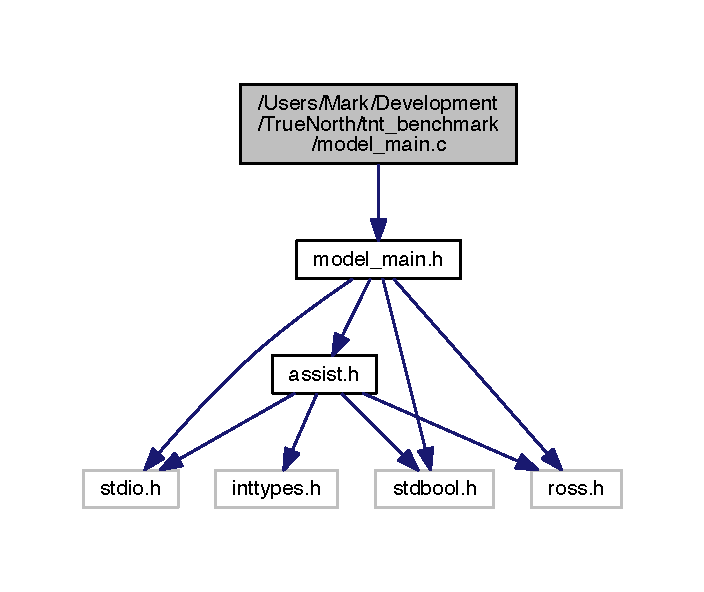
\includegraphics[width=338pt]{model__main_8c__incl}
\end{center}
\end{figure}
\subsection*{Functions}
\begin{DoxyCompactItemize}
\item 
int \hyperlink{model__main_8c_ae66f6b31b5ad750f1fe042a706a4e3d4}{main} ()
\end{DoxyCompactItemize}


\subsection{Function Documentation}
\hypertarget{model__main_8c_ae66f6b31b5ad750f1fe042a706a4e3d4}{}\index{model\+\_\+main.\+c@{model\+\_\+main.\+c}!main@{main}}
\index{main@{main}!model\+\_\+main.\+c@{model\+\_\+main.\+c}}
\subsubsection[{main}]{\setlength{\rightskip}{0pt plus 5cm}int main (
\begin{DoxyParamCaption}
{}
\end{DoxyParamCaption}
)}\label{model__main_8c_ae66f6b31b5ad750f1fe042a706a4e3d4}


Definition at line \hyperlink{model__main_8c_source_l00011}{11} of file \hyperlink{model__main_8c_source}{model\+\_\+main.\+c}.


\begin{DoxyCode}
00011            \{
00012     \textcolor{keywordflow}{return} 0;
00013 \}
\end{DoxyCode}

\hypertarget{model__main_8c_source}{}\section{/\+Users/\+Mark/\+Development/\+True\+North/tnt\+\_\+benchmark/model\+\_\+main.c}

\begin{DoxyCode}
00001 \textcolor{comment}{//}
00002 \textcolor{comment}{//  model\_main.c}
00003 \textcolor{comment}{//  ROSS\_TOP}
00004 \textcolor{comment}{//}
00005 \textcolor{comment}{//  Created by Mark Plagge on 6/17/15.}
00006 \textcolor{comment}{//}
00007 \textcolor{comment}{//}
00008 
00009 \textcolor{preprocessor}{#}\textcolor{preprocessor}{include} \hyperlink{model__main_8h}{"model\_main.h"}
00010 
\hypertarget{model__main_8c_source_l00011}{}\hyperlink{model__main_8c_ae66f6b31b5ad750f1fe042a706a4e3d4}{00011} \textcolor{keywordtype}{int} \hyperlink{model__main_8c_ae66f6b31b5ad750f1fe042a706a4e3d4}{main}() \{
00012     \textcolor{keywordflow}{return} 0;
00013 \}
\end{DoxyCode}

\hypertarget{model__main_8h}{}\section{/\+Users/\+Mark/\+Development/\+True\+North/tnt\+\_\+benchmark/model\+\_\+main.h File Reference}
\label{model__main_8h}\index{/\+Users/\+Mark/\+Development/\+True\+North/tnt\+\_\+benchmark/model\+\_\+main.\+h@{/\+Users/\+Mark/\+Development/\+True\+North/tnt\+\_\+benchmark/model\+\_\+main.\+h}}
{\ttfamily \#include \char`\"{}models/neuron\+\_\+model.\+h\char`\"{}}\\*
{\ttfamily \#include \char`\"{}models/synapse.\+h\char`\"{}}\\*
{\ttfamily \#include \char`\"{}assist.\+h\char`\"{}}\\*
{\ttfamily \#include \char`\"{}ross.\+h\char`\"{}}\\*
{\ttfamily \#include \char`\"{}spike\+\_\+generator.\+h\char`\"{}}\\*
{\ttfamily \#include \char`\"{}libs/sqlite3.\+h\char`\"{}}\\*
{\ttfamily \#include $<$stdio.\+h$>$}\\*
Include dependency graph for model\+\_\+main.\+h\+:\nopagebreak
\begin{figure}[H]
\begin{center}
\leavevmode
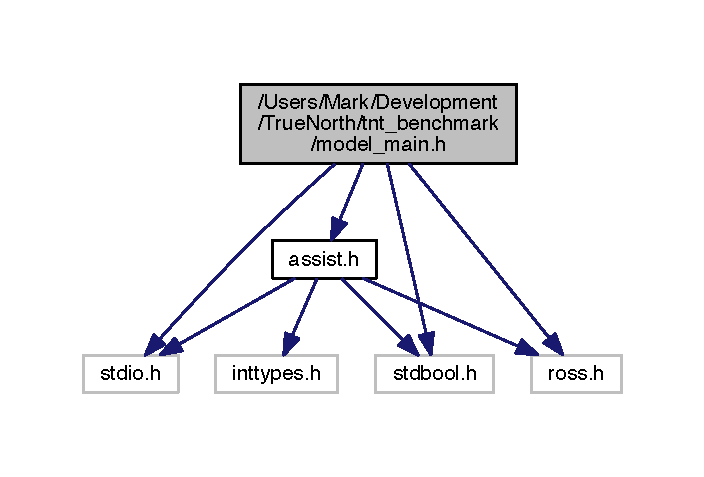
\includegraphics[width=350pt]{model__main_8h__incl}
\end{center}
\end{figure}
This graph shows which files directly or indirectly include this file\+:\nopagebreak
\begin{figure}[H]
\begin{center}
\leavevmode
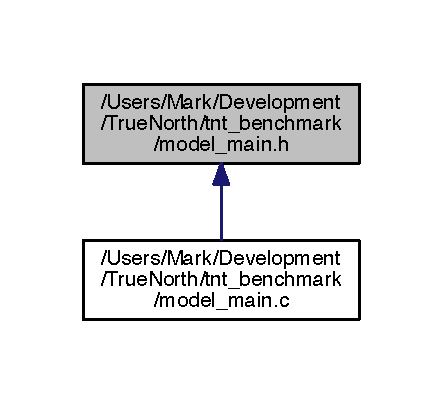
\includegraphics[width=212pt]{model__main_8h__dep__incl}
\end{center}
\end{figure}
\subsection*{Functions}
\begin{DoxyCompactItemize}
\item 
void \hyperlink{model__main_8h_a7a8df3f99e1d582c6c136b16d6e34d13}{pre\+\_\+run} ()
\item 
void \hyperlink{model__main_8h_a9309446aa05714b141a3d3caae4254db}{neuron\+\_\+event} (\hyperlink{structneuron_state}{neuron\+State} $\ast$s, tw\+\_\+bf $\ast$C\+V, \hyperlink{struct_msg___data}{Msg\+\_\+\+Data} $\ast$M, tw\+\_\+lp $\ast$lp)
\item 
void \hyperlink{model__main_8h_aea7de5bc5028e2df35cf3fe64f6cca6c}{synapse\+\_\+event} (\hyperlink{structsynapse_state}{synapse\+State} $\ast$s, tw\+\_\+bf $\ast$, \hyperlink{struct_msg___data}{Msg\+\_\+\+Data} $\ast$M, tw\+\_\+lp $\ast$lp)
\item 
void \hyperlink{model__main_8h_a8022723eba89664cca80e179b80a2b37}{neuron\+\_\+init} (\hyperlink{structneuron_state}{neuron\+State} $\ast$s, tw\+\_\+lp $\ast$lp)
\item 
void \hyperlink{model__main_8h_a579d8e5af0b1c0a80c8e83b7a534f873}{synapse\+\_\+init} (\hyperlink{structsynapse_state}{synapse\+State} $\ast$s, tw\+\_\+lp $\ast$lp)
\item 
void \hyperlink{model__main_8h_a801f93205937969fea2eff0bf2e76de9}{set\+Synapse\+Weight} (\hyperlink{structneuron_state}{neuron\+State} $\ast$s, tw\+\_\+lp $\ast$lp, int synapse\+I\+D)
\item 
void \hyperlink{model__main_8h_a4bd8bcd9c6de148a9f5c84fadd51106c}{neuron\+\_\+reverse} (\hyperlink{structneuron_state}{neuron\+State} $\ast$, tw\+\_\+bf $\ast$, \hyperlink{struct_msg___data}{Msg\+\_\+\+Data} $\ast$, tw\+\_\+lp $\ast$)
\item 
void \hyperlink{model__main_8h_a36fba0f7780630192391905fb40470cc}{synapse\+\_\+reverse} (\hyperlink{structneuron_state}{neuron\+State} $\ast$, tw\+\_\+bf $\ast$, \hyperlink{struct_msg___data}{Msg\+\_\+\+Data} $\ast$, tw\+\_\+lp $\ast$)
\item 
void \hyperlink{model__main_8h_a1f668d7246282bb6f62de09f934bee56}{synapse\+In} (int synapse\+I\+D, \hyperlink{structneuron_state}{neuron\+State} $\ast$s)
\item 
void \hyperlink{model__main_8h_a3b6bb8c3f517cbc71b3a12379f286c7f}{calculate\+Threshold} (int synapse\+I\+D, \hyperlink{structneuron_state}{neuron\+State} $\ast$s)
\item 
void \hyperlink{model__main_8h_ad3022d255395cdd5ce59a7a210232805}{check\+Fire} (int synapse\+I\+D, \hyperlink{structneuron_state}{neuron\+State} $\ast$s)
\item 
void \hyperlink{model__main_8h_acac9e41bea7d1d0911a0220de60a37b0}{neuron\+\_\+final} (\hyperlink{structneuron_state}{neuron\+State} $\ast$s, tw\+\_\+lp $\ast$lp)
\item 
void \hyperlink{model__main_8h_a3d695e7995cce87a03d6407d801e043d}{synapse\+\_\+final} (\hyperlink{structsynapse_state}{synapse\+State} $\ast$s, tw\+\_\+lp $\ast$lp)
\item 
void \hyperlink{model__main_8h_a90307b42f2863f00eb0d4290e576e0d2}{gen\+\_\+init} (\hyperlink{structspike_gen_state}{spike\+Gen\+State} $\ast$gen\+\_\+state, tw\+\_\+lp $\ast$lp)
\item 
void \hyperlink{model__main_8h_a9f6f8d34d84c91c98139da79b73a5996}{gen\+\_\+pre} (\hyperlink{structspike_gen_state}{spike\+Gen\+State} $\ast$gen\+\_\+state, tw\+\_\+lp $\ast$lp)
\item 
void \hyperlink{model__main_8h_a9b676e87fee87da0053e1af467a663da}{gen\+\_\+event} (\hyperlink{structspike_gen_state}{spike\+Gen\+State} $\ast$gen\+\_\+state, tw\+\_\+lp $\ast$lp)
\item 
void \hyperlink{model__main_8h_a655eec05ddf277450c550f96853a9799}{gen\+\_\+reverse} (\hyperlink{structspike_gen_state}{spike\+Gen\+State} $\ast$gen\+\_\+state, tw\+\_\+lp $\ast$lp)
\item 
void \hyperlink{model__main_8h_a8d028b3e829d2f44994be14d1cdcf84b}{gen\+\_\+final} (\hyperlink{structspike_gen_state}{spike\+Gen\+State} $\ast$gen\+\_\+state, tw\+\_\+lp $\ast$lp)
\item 
void \hyperlink{model__main_8h_a37439d03a72ad06efda28e7783dcc958}{get\+Local\+I\+Ds} (\hyperlink{mappings_8c_a672b405f17d1859fc9e26f09afe9a366}{gid\+\_\+t} global, \hyperlink{mappings_8c_ac35d555a6883d7624a8fc918f6cc91c0}{regid\+\_\+t} $\ast$core, \hyperlink{mappings_8c_ac35d555a6883d7624a8fc918f6cc91c0}{regid\+\_\+t} $\ast$local)
\begin{DoxyCompactList}\small\item\em Given a global I\+D, return the core number. \end{DoxyCompactList}\item 
\hyperlink{mappings_8c_a672b405f17d1859fc9e26f09afe9a366}{gid\+\_\+t} \hyperlink{model__main_8h_aba4107cb441dd8f8732f72c359a691c4}{global\+I\+D} (\hyperlink{mappings_8c_ac35d555a6883d7624a8fc918f6cc91c0}{regid\+\_\+t} core, \hyperlink{mappings_8c_ac35d555a6883d7624a8fc918f6cc91c0}{regid\+\_\+t} local)
\item 
void \hyperlink{model__main_8h_aa30d3f27017c4332fce3dca3ce944a67}{init\+Random\+Wts} (\hyperlink{structneuron_state}{neuron\+State} $\ast$s, tw\+\_\+lp $\ast$lp)
\begin{DoxyCompactList}\small\item\em neuron init helper functions\+: \end{DoxyCompactList}\item 
void \hyperlink{model__main_8h_aca6527a1ad95c75e8a0ba7d0b30b49fb}{init\+Random\+Recurrance} (\hyperlink{structneuron_state}{neuron\+State} $\ast$s)
\item 
void \hyperlink{model__main_8h_a4d92cef623a227e757b28c6068cf806c}{set\+Neuron\+Threshold} (\hyperlink{structneuron_state}{neuron\+State} $\ast$s, tw\+\_\+lp $\ast$lp)
\begin{DoxyCompactList}\small\item\em set\+Neuron\+Threshold -\/ Sets the threshold value of the neuron. \end{DoxyCompactList}\item 
void \hyperlink{model__main_8h_adb8d460fbe64ef0fdeb18a822e4e17fa}{init\+Neruon\+With\+Map} (\hyperlink{structneuron_state}{neuron\+State} $\ast$s, tw\+\_\+lp $\ast$lp, tw\+\_\+pe $\ast$pe)
\item 
void \hyperlink{model__main_8h_a1c2ffbc27679a309adf4732931990532}{init\+Synapse\+With\+Map} (\hyperlink{structneuron_state}{neuron\+State} $\ast$s, tw\+\_\+lp $\ast$lp, tw\+\_\+pe $\ast$pe)
\begin{DoxyCompactList}\small\item\em init\+Synapse\+With\+Map -- Initializes this particular synapse based on the sqllite map. \end{DoxyCompactList}\end{DoxyCompactItemize}
\subsection*{Variables}
\begin{DoxyCompactItemize}
\item 
int \hyperlink{model__main_8h_a67e8e45768f76b984a60fcff2b7c51aa}{N\+E\+U\+R\+O\+N\+S\+\_\+\+I\+N\+\_\+\+C\+O\+R\+E} = 4
\begin{DoxyCompactList}\small\item\em Number of neurons per core. \end{DoxyCompactList}\item 
int \hyperlink{model__main_8h_a076b99099b46431255982b2bb8ce06fb}{S\+Y\+N\+A\+P\+S\+E\+S\+\_\+\+I\+N\+\_\+\+C\+O\+R\+E} = 8
\begin{DoxyCompactList}\small\item\em Number of synapses per core. \end{DoxyCompactList}\item 
int \hyperlink{model__main_8h_a851557110b7442a40078d6ef85c2de76}{C\+O\+R\+E\+S\+\_\+\+P\+E\+R\+\_\+\+P\+E} = 2
\begin{DoxyCompactList}\small\item\em Each P\+E can have one or more virtual cores running during the simulation. \end{DoxyCompactList}\item 
int \hyperlink{model__main_8h_a433873baf41da436ba9c1734c8c5ddd2}{T\+H\+R\+E\+S\+H\+O\+L\+D\+\_\+\+M\+A\+X} = 11
\begin{DoxyCompactList}\small\item\em Determines the maximum and minimum thresholds for a neuron to fire. \end{DoxyCompactList}\item 
int \hyperlink{model__main_8h_a55f4484944f4174b5e677c0a71b30e4a}{T\+H\+R\+E\+S\+H\+O\+L\+D\+\_\+\+M\+I\+N} = 5
\begin{DoxyCompactList}\small\item\em Minimum threshold. \end{DoxyCompactList}\item 
int \hyperlink{model__main_8h_a20ef6d41d2f384358522fb59fb6226cb}{S\+Y\+N\+A\+P\+S\+E\+\_\+\+W\+E\+I\+G\+H\+T\+\_\+\+M\+A\+X} = 10
\begin{DoxyCompactList}\small\item\em Each neuron is connected to the synapses (inputs) within the core it is running in. \end{DoxyCompactList}\item 
int \hyperlink{model__main_8h_af38a0e2e2483ef81f7ea5175c366ce82}{S\+Y\+N\+A\+P\+S\+E\+\_\+\+W\+E\+I\+G\+H\+T\+\_\+\+M\+I\+N} = 5
\begin{DoxyCompactList}\small\item\em Minimum synapse weight. \end{DoxyCompactList}\item 
int \hyperlink{model__main_8h_ad39b86a0b748731175572436f6672264}{C\+O\+R\+E\+\_\+\+S\+I\+Z\+E}
\item 
float \hyperlink{model__main_8h_a0cd5ccf63b6dd9b12098d82503d03c05}{C\+L\+O\+C\+K\+\_\+\+S\+P\+E\+E\+D} = 1
\item 
int \hyperlink{model__main_8h_a8f579325f29e8089879da11747d83c96}{G\+E\+N\+\_\+\+L\+A\+G} = 1000
\item 
bool \hyperlink{model__main_8h_ac18d5985ff9fbfe912f1336eaa82ead6}{U\+S\+E\+\_\+\+O\+T\+H\+E\+R\+\_\+\+L\+E\+A\+K\+S} = false
\item 
bool \hyperlink{model__main_8h_a2a2a6154f99c6f9aa80e1afdcdc8d0d6}{U\+S\+E\+\_\+\+O\+T\+H\+E\+R\+\_\+\+R\+E\+S\+E\+T} = false
\item 
int \hyperlink{model__main_8h_abf39b7bc925f61737112787c578b06d3}{M\+I\+N\+\_\+\+L\+E\+A\+K} = 0
\item 
int \hyperlink{model__main_8h_a83c9373146a1150aa913c244e69abcaa}{M\+A\+X\+\_\+\+L\+E\+A\+K} = 10
\item 
char $\ast$ \hyperlink{model__main_8h_aa7b16932280ed0b12a0b4e7d675aac25}{A\+L\+T\+\_\+\+L\+E\+A\+K}
\item 
char $\ast$ \hyperlink{model__main_8h_a4c27ccb8c2f6992dcb9a961cc45e69a1}{A\+L\+T\+\_\+\+R\+E\+S\+E\+T}
\item 
int \hyperlink{model__main_8h_a789de05c7ed7a8cfadbd6b2e0c75516c}{M\+I\+N\+\_\+\+R\+E\+S\+E\+T} = 0
\item 
int \hyperlink{model__main_8h_ad6e4d5bfe16dc8db2633d5687661cfc8}{M\+A\+X\+\_\+\+R\+E\+S\+E\+T} = 10
\item 
int \hyperlink{model__main_8h_ac858bb435ac6b897dd949dbfdc61b5a5}{D\+E\+B\+U\+G\+\_\+\+M\+O\+D\+E} = 0
\item 
char $\ast$ \hyperlink{model__main_8h_a4e253d6390edbb51c63eac572d72b97a}{config\+File\+Path}
\item 
bool \hyperlink{model__main_8h_a002a2a64f4efdb283983d95f46f92596}{is\+File}
\item 
tw\+\_\+stime \hyperlink{model__main_8h_ac877337ae1e75d1b6640f41799f5a72c}{lookahead} = .\+00000000001
\item 
int \hyperlink{model__main_8h_a47d27feae0fedebece9a496a627122b9}{events\+\_\+per\+\_\+pe} = 0
\item 
int \hyperlink{model__main_8h_aaf6452b3f3c110587b95a22cf85b364a}{E\+X\+E\+C\+\_\+\+M\+E\+M\+O\+R\+Y} = 100000000
\item 
int \hyperlink{model__main_8h_a31c1ceb0e0910a3bc41f26c66252b321}{C\+L\+O\+C\+K\+\_\+\+R\+A\+T\+E} = 10
\item 
int \hyperlink{model__main_8h_aaa8f238cc23dfaa638510e226aad9df6}{tt\+\_\+neurons} = 0
\item 
int \hyperlink{model__main_8h_abb2a31424ba8aab7f54e79ae2cba5859}{tt\+\_\+synapses} = 0
\item 
bool \hyperlink{model__main_8h_ad65c1aa107c6fb135e0a75ecc78d52b2}{G\+E\+N\+\_\+\+O\+N} = 1
\begin{DoxyCompactList}\small\item\em Generator Options. \end{DoxyCompactList}\item 
bool \hyperlink{model__main_8h_ab42fd7d6d043114d1147acc77bd7e867}{G\+E\+N\+\_\+\+R\+N\+D} = 1
\item 
int \hyperlink{model__main_8h_a24519e41d61089dd8c7107f1cfe56ac2}{R\+N\+D\+\_\+\+M\+O\+D\+E} = 0
\item 
unsigned int \hyperlink{model__main_8h_a4875b976acd12ff43cc03898be994253}{G\+E\+N\+\_\+\+P\+R\+O\+B} = 50
\item 
unsigned int \hyperlink{model__main_8h_a3ba8de640782035ea9e91ab791d9f14f}{G\+E\+N\+\_\+\+F\+C\+T} = 5
\item 
int \hyperlink{model__main_8h_a4acc05ba6639c20420024881b69a585d}{G\+E\+N\+\_\+\+O\+U\+T\+B\+O\+U\+N\+D} = 4
\item 
const tw\+\_\+optdef \hyperlink{model__main_8h_ada0c7e7c55b61581d8fec48f6cf842b7}{app\+\_\+opt} \mbox{[}$\,$\mbox{]}
\item 
tw\+\_\+lptype \hyperlink{model__main_8h_a6acf8f296294224aa8201bdea5aba47e}{model\+\_\+lps} \mbox{[}$\,$\mbox{]}
\end{DoxyCompactItemize}


\subsection{Function Documentation}
\hypertarget{model__main_8h_a3b6bb8c3f517cbc71b3a12379f286c7f}{}\index{model\+\_\+main.\+h@{model\+\_\+main.\+h}!calculate\+Threshold@{calculate\+Threshold}}
\index{calculate\+Threshold@{calculate\+Threshold}!model\+\_\+main.\+h@{model\+\_\+main.\+h}}
\subsubsection[{calculate\+Threshold}]{\setlength{\rightskip}{0pt plus 5cm}void calculate\+Threshold (
\begin{DoxyParamCaption}
\item[{int}]{synapse\+I\+D, }
\item[{{\bf neuron\+State} $\ast$}]{s}
\end{DoxyParamCaption}
)}\label{model__main_8h_a3b6bb8c3f517cbc71b3a12379f286c7f}
\hypertarget{model__main_8h_ad3022d255395cdd5ce59a7a210232805}{}\index{model\+\_\+main.\+h@{model\+\_\+main.\+h}!check\+Fire@{check\+Fire}}
\index{check\+Fire@{check\+Fire}!model\+\_\+main.\+h@{model\+\_\+main.\+h}}
\subsubsection[{check\+Fire}]{\setlength{\rightskip}{0pt plus 5cm}void check\+Fire (
\begin{DoxyParamCaption}
\item[{int}]{synapse\+I\+D, }
\item[{{\bf neuron\+State} $\ast$}]{s}
\end{DoxyParamCaption}
)}\label{model__main_8h_ad3022d255395cdd5ce59a7a210232805}
\hypertarget{model__main_8h_a9b676e87fee87da0053e1af467a663da}{}\index{model\+\_\+main.\+h@{model\+\_\+main.\+h}!gen\+\_\+event@{gen\+\_\+event}}
\index{gen\+\_\+event@{gen\+\_\+event}!model\+\_\+main.\+h@{model\+\_\+main.\+h}}
\subsubsection[{gen\+\_\+event}]{\setlength{\rightskip}{0pt plus 5cm}void gen\+\_\+event (
\begin{DoxyParamCaption}
\item[{{\bf spike\+Gen\+State} $\ast$}]{gen\+\_\+state, }
\item[{tw\+\_\+lp $\ast$}]{lp}
\end{DoxyParamCaption}
)}\label{model__main_8h_a9b676e87fee87da0053e1af467a663da}
\hypertarget{model__main_8h_a8d028b3e829d2f44994be14d1cdcf84b}{}\index{model\+\_\+main.\+h@{model\+\_\+main.\+h}!gen\+\_\+final@{gen\+\_\+final}}
\index{gen\+\_\+final@{gen\+\_\+final}!model\+\_\+main.\+h@{model\+\_\+main.\+h}}
\subsubsection[{gen\+\_\+final}]{\setlength{\rightskip}{0pt plus 5cm}void gen\+\_\+final (
\begin{DoxyParamCaption}
\item[{{\bf spike\+Gen\+State} $\ast$}]{gen\+\_\+state, }
\item[{tw\+\_\+lp $\ast$}]{lp}
\end{DoxyParamCaption}
)}\label{model__main_8h_a8d028b3e829d2f44994be14d1cdcf84b}
\hypertarget{model__main_8h_a90307b42f2863f00eb0d4290e576e0d2}{}\index{model\+\_\+main.\+h@{model\+\_\+main.\+h}!gen\+\_\+init@{gen\+\_\+init}}
\index{gen\+\_\+init@{gen\+\_\+init}!model\+\_\+main.\+h@{model\+\_\+main.\+h}}
\subsubsection[{gen\+\_\+init}]{\setlength{\rightskip}{0pt plus 5cm}void gen\+\_\+init (
\begin{DoxyParamCaption}
\item[{{\bf spike\+Gen\+State} $\ast$}]{gen\+\_\+state, }
\item[{tw\+\_\+lp $\ast$}]{lp}
\end{DoxyParamCaption}
)}\label{model__main_8h_a90307b42f2863f00eb0d4290e576e0d2}
\hypertarget{model__main_8h_a9f6f8d34d84c91c98139da79b73a5996}{}\index{model\+\_\+main.\+h@{model\+\_\+main.\+h}!gen\+\_\+pre@{gen\+\_\+pre}}
\index{gen\+\_\+pre@{gen\+\_\+pre}!model\+\_\+main.\+h@{model\+\_\+main.\+h}}
\subsubsection[{gen\+\_\+pre}]{\setlength{\rightskip}{0pt plus 5cm}void gen\+\_\+pre (
\begin{DoxyParamCaption}
\item[{{\bf spike\+Gen\+State} $\ast$}]{gen\+\_\+state, }
\item[{tw\+\_\+lp $\ast$}]{lp}
\end{DoxyParamCaption}
)}\label{model__main_8h_a9f6f8d34d84c91c98139da79b73a5996}
\hypertarget{model__main_8h_a655eec05ddf277450c550f96853a9799}{}\index{model\+\_\+main.\+h@{model\+\_\+main.\+h}!gen\+\_\+reverse@{gen\+\_\+reverse}}
\index{gen\+\_\+reverse@{gen\+\_\+reverse}!model\+\_\+main.\+h@{model\+\_\+main.\+h}}
\subsubsection[{gen\+\_\+reverse}]{\setlength{\rightskip}{0pt plus 5cm}void gen\+\_\+reverse (
\begin{DoxyParamCaption}
\item[{{\bf spike\+Gen\+State} $\ast$}]{gen\+\_\+state, }
\item[{tw\+\_\+lp $\ast$}]{lp}
\end{DoxyParamCaption}
)}\label{model__main_8h_a655eec05ddf277450c550f96853a9799}
\hypertarget{model__main_8h_a37439d03a72ad06efda28e7783dcc958}{}\index{model\+\_\+main.\+h@{model\+\_\+main.\+h}!get\+Local\+I\+Ds@{get\+Local\+I\+Ds}}
\index{get\+Local\+I\+Ds@{get\+Local\+I\+Ds}!model\+\_\+main.\+h@{model\+\_\+main.\+h}}
\subsubsection[{get\+Local\+I\+Ds}]{\setlength{\rightskip}{0pt plus 5cm}void get\+Local\+I\+Ds (
\begin{DoxyParamCaption}
\item[{{\bf gid\+\_\+t}}]{global, }
\item[{{\bf regid\+\_\+t} $\ast$}]{core, }
\item[{{\bf regid\+\_\+t} $\ast$}]{local}
\end{DoxyParamCaption}
)}\label{model__main_8h_a37439d03a72ad06efda28e7783dcc958}


Given a global I\+D, return the core number. 

Given a global I\+D, return the core number. 

Definition at line 22 of file mappings.\+c.



Referenced by test\+Val().


\begin{DoxyCode}
22                                                                \{
23     (*core) = \hyperlink{mappings_8c_a5bf12e6001846798b26182c47c53df9b}{CORE}(global);
24     (*local)= \hyperlink{mappings_8c_a83bb0fed7e64e381d564a9f1cb951fac}{LOC}(global);
25 \}
\end{DoxyCode}
\hypertarget{model__main_8h_aba4107cb441dd8f8732f72c359a691c4}{}\index{model\+\_\+main.\+h@{model\+\_\+main.\+h}!global\+I\+D@{global\+I\+D}}
\index{global\+I\+D@{global\+I\+D}!model\+\_\+main.\+h@{model\+\_\+main.\+h}}
\subsubsection[{global\+I\+D}]{\setlength{\rightskip}{0pt plus 5cm}{\bf gid\+\_\+t} global\+I\+D (
\begin{DoxyParamCaption}
\item[{{\bf regid\+\_\+t}}]{core, }
\item[{{\bf regid\+\_\+t}}]{local}
\end{DoxyParamCaption}
)}\label{model__main_8h_aba4107cb441dd8f8732f72c359a691c4}


Definition at line 26 of file mappings.\+c.



Referenced by main(), and test\+Val().


\begin{DoxyCode}
26                                            \{
27     \hyperlink{mappings_8c_a672b405f17d1859fc9e26f09afe9a366}{gid\_t} returnVal = 0;
28     returnVal = ((uint64\_t)core << 32) | local;
29     \textcolor{keywordflow}{return} returnVal;
30 \}
\end{DoxyCode}
\hypertarget{model__main_8h_adb8d460fbe64ef0fdeb18a822e4e17fa}{}\index{model\+\_\+main.\+h@{model\+\_\+main.\+h}!init\+Neruon\+With\+Map@{init\+Neruon\+With\+Map}}
\index{init\+Neruon\+With\+Map@{init\+Neruon\+With\+Map}!model\+\_\+main.\+h@{model\+\_\+main.\+h}}
\subsubsection[{init\+Neruon\+With\+Map}]{\setlength{\rightskip}{0pt plus 5cm}void init\+Neruon\+With\+Map (
\begin{DoxyParamCaption}
\item[{{\bf neuron\+State} $\ast$}]{s, }
\item[{tw\+\_\+lp $\ast$}]{lp, }
\item[{tw\+\_\+pe $\ast$}]{pe}
\end{DoxyParamCaption}
)}\label{model__main_8h_adb8d460fbe64ef0fdeb18a822e4e17fa}
\hypertarget{model__main_8h_aca6527a1ad95c75e8a0ba7d0b30b49fb}{}\index{model\+\_\+main.\+h@{model\+\_\+main.\+h}!init\+Random\+Recurrance@{init\+Random\+Recurrance}}
\index{init\+Random\+Recurrance@{init\+Random\+Recurrance}!model\+\_\+main.\+h@{model\+\_\+main.\+h}}
\subsubsection[{init\+Random\+Recurrance}]{\setlength{\rightskip}{0pt plus 5cm}void init\+Random\+Recurrance (
\begin{DoxyParamCaption}
\item[{{\bf neuron\+State} $\ast$}]{s}
\end{DoxyParamCaption}
)}\label{model__main_8h_aca6527a1ad95c75e8a0ba7d0b30b49fb}
\hypertarget{model__main_8h_aa30d3f27017c4332fce3dca3ce944a67}{}\index{model\+\_\+main.\+h@{model\+\_\+main.\+h}!init\+Random\+Wts@{init\+Random\+Wts}}
\index{init\+Random\+Wts@{init\+Random\+Wts}!model\+\_\+main.\+h@{model\+\_\+main.\+h}}
\subsubsection[{init\+Random\+Wts}]{\setlength{\rightskip}{0pt plus 5cm}void init\+Random\+Wts (
\begin{DoxyParamCaption}
\item[{{\bf neuron\+State} $\ast$}]{s, }
\item[{tw\+\_\+lp $\ast$}]{lp}
\end{DoxyParamCaption}
)}\label{model__main_8h_aa30d3f27017c4332fce3dca3ce944a67}


neuron init helper functions\+: 

neuron init helper functions\+:

Essentially creates a randomized neural network if called on all new neurons. 
\begin{DoxyParams}{Parameters}
{\em $\ast$s} & The new neuron, created by R\+O\+S\+S indirectly. \\
\hline
\end{DoxyParams}


Definition at line 98 of file model\+\_\+main.\+c.



References neuron\+State\+::per\+Synapse\+Det, and S\+Y\+N\+A\+P\+S\+E\+S\+\_\+\+I\+N\+\_\+\+C\+O\+R\+E.


\begin{DoxyCode}
98                                              \{
99     s->\hyperlink{structneuron_state_a95688135a244a3ce3b35698a49d0da18}{perSynapseDet} = tw\_calloc(\textcolor{stringliteral}{"Error-SynapseWeightInit"} , 81, \textcolor{stringliteral}{"Neurons"}, \textcolor{keyword}{sizeof}(\textcolor{keywordtype}{bool}), 
      \hyperlink{assist_8h_a076b99099b46431255982b2bb8ce06fb}{SYNAPSES\_IN\_CORE});
100     s->\hyperlink{structneuron_state_ac21457aec3f29f9f28b58dd95e3d6fb2}{perSynapseWeight} = tw\_calloc(\textcolor{stringliteral}{"Error-SynapseWeightInit"} , 81, \textcolor{stringliteral}{"Neurons"}, \textcolor{keyword}{sizeof}(
      \hyperlink{assist_8h_a368ddcd71f7b61cb0f918f22d07ce999}{\_neVoltType}), \hyperlink{assist_8h_a076b99099b46431255982b2bb8ce06fb}{SYNAPSES\_IN\_CORE});
101         \textcolor{comment}{//randomized wts:}
102     \textcolor{keywordflow}{for}(\textcolor{keywordtype}{int} j = 0; j < \hyperlink{assist_8h_a076b99099b46431255982b2bb8ce06fb}{SYNAPSES\_IN\_CORE}; j ++)\{
103         s->\hyperlink{structneuron_state_a95688135a244a3ce3b35698a49d0da18}{perSynapseDet}[j] = \textcolor{keyword}{true};
104         s->\hyperlink{structneuron_state_ac21457aec3f29f9f28b58dd95e3d6fb2}{perSynapseWeight}[j] = tw\_rand\_integer(lp->rng, 0, 
      \hyperlink{assist_8h_a20ef6d41d2f384358522fb59fb6226cb}{SYNAPSE\_WEIGHT\_MAX});
105     \}
106 \}
\end{DoxyCode}
\hypertarget{model__main_8h_a1c2ffbc27679a309adf4732931990532}{}\index{model\+\_\+main.\+h@{model\+\_\+main.\+h}!init\+Synapse\+With\+Map@{init\+Synapse\+With\+Map}}
\index{init\+Synapse\+With\+Map@{init\+Synapse\+With\+Map}!model\+\_\+main.\+h@{model\+\_\+main.\+h}}
\subsubsection[{init\+Synapse\+With\+Map}]{\setlength{\rightskip}{0pt plus 5cm}void init\+Synapse\+With\+Map (
\begin{DoxyParamCaption}
\item[{{\bf neuron\+State} $\ast$}]{s, }
\item[{tw\+\_\+lp $\ast$}]{lp, }
\item[{tw\+\_\+pe $\ast$}]{pe}
\end{DoxyParamCaption}
)}\label{model__main_8h_a1c2ffbc27679a309adf4732931990532}


init\+Synapse\+With\+Map -- Initializes this particular synapse based on the sqllite map. 

See \hyperlink{model__main_8c_a266b9268757e9418220da53a9a12ff43}{init\+Neuron\+With\+Map()} for more information. 

Definition at line 119 of file model\+\_\+main.\+c.


\begin{DoxyCode}
119                                                               \{
120      printf(\textcolor{stringliteral}{"not implemented yet"});
121  \}
\end{DoxyCode}
\hypertarget{model__main_8h_a9309446aa05714b141a3d3caae4254db}{}\index{model\+\_\+main.\+h@{model\+\_\+main.\+h}!neuron\+\_\+event@{neuron\+\_\+event}}
\index{neuron\+\_\+event@{neuron\+\_\+event}!model\+\_\+main.\+h@{model\+\_\+main.\+h}}
\subsubsection[{neuron\+\_\+event}]{\setlength{\rightskip}{0pt plus 5cm}void neuron\+\_\+event (
\begin{DoxyParamCaption}
\item[{{\bf neuron\+State} $\ast$}]{s, }
\item[{tw\+\_\+bf $\ast$}]{C\+V, }
\item[{{\bf Msg\+\_\+\+Data} $\ast$}]{M, }
\item[{tw\+\_\+lp $\ast$}]{lp}
\end{DoxyParamCaption}
)}\label{model__main_8h_a9309446aa05714b141a3d3caae4254db}
\hypertarget{model__main_8h_acac9e41bea7d1d0911a0220de60a37b0}{}\index{model\+\_\+main.\+h@{model\+\_\+main.\+h}!neuron\+\_\+final@{neuron\+\_\+final}}
\index{neuron\+\_\+final@{neuron\+\_\+final}!model\+\_\+main.\+h@{model\+\_\+main.\+h}}
\subsubsection[{neuron\+\_\+final}]{\setlength{\rightskip}{0pt plus 5cm}void neuron\+\_\+final (
\begin{DoxyParamCaption}
\item[{{\bf neuron\+State} $\ast$}]{s, }
\item[{tw\+\_\+lp $\ast$}]{lp}
\end{DoxyParamCaption}
)}\label{model__main_8h_acac9e41bea7d1d0911a0220de60a37b0}
\hypertarget{model__main_8h_a8022723eba89664cca80e179b80a2b37}{}\index{model\+\_\+main.\+h@{model\+\_\+main.\+h}!neuron\+\_\+init@{neuron\+\_\+init}}
\index{neuron\+\_\+init@{neuron\+\_\+init}!model\+\_\+main.\+h@{model\+\_\+main.\+h}}
\subsubsection[{neuron\+\_\+init}]{\setlength{\rightskip}{0pt plus 5cm}void neuron\+\_\+init (
\begin{DoxyParamCaption}
\item[{{\bf neuron\+State} $\ast$}]{s, }
\item[{tw\+\_\+lp $\ast$}]{lp}
\end{DoxyParamCaption}
)}\label{model__main_8h_a8022723eba89664cca80e179b80a2b37}


Definition at line 44 of file model\+\_\+main.\+c.



References neuron\+State\+::fire\+Count, is\+File, neuron\+State\+::leak\+Rate, and neuron\+State\+::pr\+Voltage.


\begin{DoxyCode}
44                                             \{
45     tw\_lpid \textcolor{keyword}{self} = lp->gid;
46 
47         \textcolor{comment}{//set neuron local id}
48     s->\hyperlink{structneuron_state_acc19e6f856ad128cc1f90527d066700b}{coreID} = \hyperlink{assist_8h_a5bf12e6001846798b26182c47c53df9b}{CORE}(\textcolor{keyword}{self});
49     s->\hyperlink{structneuron_state_ab668c4d903557a2ac39f2a5141df3976}{neuronID} = \hyperlink{assist_8h_a83bb0fed7e64e381d564a9f1cb951fac}{LOC}(\textcolor{keyword}{self});
50         \textcolor{comment}{//initial membrane potential values}
51     s->\hyperlink{structneuron_state_ac20c9ef5b5825eb38f91c1f1dacfb21d}{prVoltage} = 0;
52     s->\hyperlink{structneuron_state_afc17c439bc3ffa469b045a7ceff7a25a}{fireCount} = 0;
53     s->\hyperlink{structneuron_state_a6f4e4d8fc1cf0257b486e01f628d2656}{lastLeakTime} = 0;
54     s->\hyperlink{structneuron_state_a0658ad1f8b57a00589c6ea84f9a4ab13}{lastActiveTime} = 0;
55         \textcolor{comment}{//benchmarking default values.}
56         \textcolor{comment}{//benchmark leak means membrane potential goes to zero after firing, and no leaks}
57     s->\hyperlink{structneuron_state_afe8da12a0fe0aef0987e785a64619706}{leakRate} = 0;
58     s->\hyperlink{structneuron_state_ad0271f69fc01192f4f85b74d9bee06de}{leak} = &\hyperlink{neuron__model_8h_a6d548f86a3f6618241b7ffc5dd3ad374}{noLeak};
59     s->\hyperlink{structneuron_state_a6f4e4d8fc1cf0257b486e01f628d2656}{lastLeakTime}= 0;
60     s->\hyperlink{structneuron_state_a0f71d6ac3efc9d397adfcc72c7fe40c1}{reverseLeak} = &\hyperlink{neuron__model_8h_a23e8b1105b7db3282e2b362edbb98f5a}{revNoLeak};
61     \textcolor{keywordflow}{if}(\hyperlink{assist_8h_a002a2a64f4efdb283983d95f46f92596}{isFile} == \textcolor{keyword}{false})\{ \textcolor{comment}{//no file map, so we use random values. For benchmark, we have to create}
62                          \textcolor{comment}{//a recurrance network.}
63         \hyperlink{model__main_8c_aa30d3f27017c4332fce3dca3ce944a67}{initRandomWts}(s, lp);
64 
65         
66 
67     \}
68         \textcolor{comment}{//using a sqlite mapping}
69     \textcolor{keywordflow}{else}\{
70 
71         initWithMap(s, lp, lp->pe);
72     \}
73 
74 
75 
76 \}
\end{DoxyCode}
\hypertarget{model__main_8h_a4bd8bcd9c6de148a9f5c84fadd51106c}{}\index{model\+\_\+main.\+h@{model\+\_\+main.\+h}!neuron\+\_\+reverse@{neuron\+\_\+reverse}}
\index{neuron\+\_\+reverse@{neuron\+\_\+reverse}!model\+\_\+main.\+h@{model\+\_\+main.\+h}}
\subsubsection[{neuron\+\_\+reverse}]{\setlength{\rightskip}{0pt plus 5cm}void neuron\+\_\+reverse (
\begin{DoxyParamCaption}
\item[{{\bf neuron\+State} $\ast$}]{, }
\item[{tw\+\_\+bf $\ast$}]{, }
\item[{{\bf Msg\+\_\+\+Data} $\ast$}]{, }
\item[{tw\+\_\+lp $\ast$}]{}
\end{DoxyParamCaption}
)}\label{model__main_8h_a4bd8bcd9c6de148a9f5c84fadd51106c}
\hypertarget{model__main_8h_a7a8df3f99e1d582c6c136b16d6e34d13}{}\index{model\+\_\+main.\+h@{model\+\_\+main.\+h}!pre\+\_\+run@{pre\+\_\+run}}
\index{pre\+\_\+run@{pre\+\_\+run}!model\+\_\+main.\+h@{model\+\_\+main.\+h}}
\subsubsection[{pre\+\_\+run}]{\setlength{\rightskip}{0pt plus 5cm}void pre\+\_\+run (
\begin{DoxyParamCaption}
{}
\end{DoxyParamCaption}
)}\label{model__main_8h_a7a8df3f99e1d582c6c136b16d6e34d13}


Definition at line 80 of file model\+\_\+main.\+c.


\begin{DoxyCode}
80                \{
81         \textcolor{comment}{//set up GID mapping here?}
82 \}
\end{DoxyCode}
\hypertarget{model__main_8h_a4d92cef623a227e757b28c6068cf806c}{}\index{model\+\_\+main.\+h@{model\+\_\+main.\+h}!set\+Neuron\+Threshold@{set\+Neuron\+Threshold}}
\index{set\+Neuron\+Threshold@{set\+Neuron\+Threshold}!model\+\_\+main.\+h@{model\+\_\+main.\+h}}
\subsubsection[{set\+Neuron\+Threshold}]{\setlength{\rightskip}{0pt plus 5cm}void set\+Neuron\+Threshold (
\begin{DoxyParamCaption}
\item[{{\bf neuron\+State} $\ast$}]{s, }
\item[{tw\+\_\+lp $\ast$}]{lp}
\end{DoxyParamCaption}
)}\label{model__main_8h_a4d92cef623a227e757b28c6068cf806c}


set\+Neuron\+Threshold -\/ Sets the threshold value of the neuron. 

If there is a map, then this will use the map\textquotesingle{}s values. Otherwise, it sets it to a random value based on the parameters \hyperlink{model__main_8h_a55f4484944f4174b5e677c0a71b30e4a}{T\+H\+R\+E\+S\+H\+O\+L\+D\+\_\+\+M\+I\+N} and \hyperlink{model__main_8h_a433873baf41da436ba9c1734c8c5ddd2}{T\+H\+R\+E\+S\+H\+O\+L\+D\+\_\+\+M\+A\+X}. 

Definition at line 129 of file model\+\_\+main.\+c.



References is\+File.


\begin{DoxyCode}
129                                                   \{
130     \textcolor{keywordflow}{if}(\hyperlink{assist_8h_a002a2a64f4efdb283983d95f46f92596}{isFile})\{
131             \textcolor{comment}{//todo: implement this sql/json/whatever file system}
132     \}
133     \textcolor{keywordflow}{else} \{
134         s->\hyperlink{structneuron_state_ac3d7ce178528ec72b94fc0698be8213a}{threshold} = tw\_rand\_integer(lp->rng, \hyperlink{assist_8h_a55f4484944f4174b5e677c0a71b30e4a}{THRESHOLD\_MIN}, 
      \hyperlink{assist_8h_a433873baf41da436ba9c1734c8c5ddd2}{THRESHOLD\_MAX});
135     \}
136 \}
\end{DoxyCode}
\hypertarget{model__main_8h_a801f93205937969fea2eff0bf2e76de9}{}\index{model\+\_\+main.\+h@{model\+\_\+main.\+h}!set\+Synapse\+Weight@{set\+Synapse\+Weight}}
\index{set\+Synapse\+Weight@{set\+Synapse\+Weight}!model\+\_\+main.\+h@{model\+\_\+main.\+h}}
\subsubsection[{set\+Synapse\+Weight}]{\setlength{\rightskip}{0pt plus 5cm}void set\+Synapse\+Weight (
\begin{DoxyParamCaption}
\item[{{\bf neuron\+State} $\ast$}]{s, }
\item[{tw\+\_\+lp $\ast$}]{lp, }
\item[{int}]{synapse\+I\+D}
\end{DoxyParamCaption}
)}\label{model__main_8h_a801f93205937969fea2eff0bf2e76de9}
\hypertarget{model__main_8h_aea7de5bc5028e2df35cf3fe64f6cca6c}{}\index{model\+\_\+main.\+h@{model\+\_\+main.\+h}!synapse\+\_\+event@{synapse\+\_\+event}}
\index{synapse\+\_\+event@{synapse\+\_\+event}!model\+\_\+main.\+h@{model\+\_\+main.\+h}}
\subsubsection[{synapse\+\_\+event}]{\setlength{\rightskip}{0pt plus 5cm}void synapse\+\_\+event (
\begin{DoxyParamCaption}
\item[{{\bf synapse\+State} $\ast$}]{s, }
\item[{tw\+\_\+bf $\ast$}]{, }
\item[{{\bf Msg\+\_\+\+Data} $\ast$}]{M, }
\item[{tw\+\_\+lp $\ast$}]{lp}
\end{DoxyParamCaption}
)}\label{model__main_8h_aea7de5bc5028e2df35cf3fe64f6cca6c}
\hypertarget{model__main_8h_a3d695e7995cce87a03d6407d801e043d}{}\index{model\+\_\+main.\+h@{model\+\_\+main.\+h}!synapse\+\_\+final@{synapse\+\_\+final}}
\index{synapse\+\_\+final@{synapse\+\_\+final}!model\+\_\+main.\+h@{model\+\_\+main.\+h}}
\subsubsection[{synapse\+\_\+final}]{\setlength{\rightskip}{0pt plus 5cm}void synapse\+\_\+final (
\begin{DoxyParamCaption}
\item[{{\bf synapse\+State} $\ast$}]{s, }
\item[{tw\+\_\+lp $\ast$}]{lp}
\end{DoxyParamCaption}
)}\label{model__main_8h_a3d695e7995cce87a03d6407d801e043d}
\hypertarget{model__main_8h_a579d8e5af0b1c0a80c8e83b7a534f873}{}\index{model\+\_\+main.\+h@{model\+\_\+main.\+h}!synapse\+\_\+init@{synapse\+\_\+init}}
\index{synapse\+\_\+init@{synapse\+\_\+init}!model\+\_\+main.\+h@{model\+\_\+main.\+h}}
\subsubsection[{synapse\+\_\+init}]{\setlength{\rightskip}{0pt plus 5cm}void synapse\+\_\+init (
\begin{DoxyParamCaption}
\item[{{\bf synapse\+State} $\ast$}]{s, }
\item[{tw\+\_\+lp $\ast$}]{lp}
\end{DoxyParamCaption}
)}\label{model__main_8h_a579d8e5af0b1c0a80c8e83b7a534f873}
\hypertarget{model__main_8h_a36fba0f7780630192391905fb40470cc}{}\index{model\+\_\+main.\+h@{model\+\_\+main.\+h}!synapse\+\_\+reverse@{synapse\+\_\+reverse}}
\index{synapse\+\_\+reverse@{synapse\+\_\+reverse}!model\+\_\+main.\+h@{model\+\_\+main.\+h}}
\subsubsection[{synapse\+\_\+reverse}]{\setlength{\rightskip}{0pt plus 5cm}void synapse\+\_\+reverse (
\begin{DoxyParamCaption}
\item[{{\bf neuron\+State} $\ast$}]{, }
\item[{tw\+\_\+bf $\ast$}]{, }
\item[{{\bf Msg\+\_\+\+Data} $\ast$}]{, }
\item[{tw\+\_\+lp $\ast$}]{}
\end{DoxyParamCaption}
)}\label{model__main_8h_a36fba0f7780630192391905fb40470cc}
\hypertarget{model__main_8h_a1f668d7246282bb6f62de09f934bee56}{}\index{model\+\_\+main.\+h@{model\+\_\+main.\+h}!synapse\+In@{synapse\+In}}
\index{synapse\+In@{synapse\+In}!model\+\_\+main.\+h@{model\+\_\+main.\+h}}
\subsubsection[{synapse\+In}]{\setlength{\rightskip}{0pt plus 5cm}void synapse\+In (
\begin{DoxyParamCaption}
\item[{int}]{synapse\+I\+D, }
\item[{{\bf neuron\+State} $\ast$}]{s}
\end{DoxyParamCaption}
)}\label{model__main_8h_a1f668d7246282bb6f62de09f934bee56}


\subsection{Variable Documentation}
\hypertarget{model__main_8h_aa7b16932280ed0b12a0b4e7d675aac25}{}\index{model\+\_\+main.\+h@{model\+\_\+main.\+h}!A\+L\+T\+\_\+\+L\+E\+A\+K@{A\+L\+T\+\_\+\+L\+E\+A\+K}}
\index{A\+L\+T\+\_\+\+L\+E\+A\+K@{A\+L\+T\+\_\+\+L\+E\+A\+K}!model\+\_\+main.\+h@{model\+\_\+main.\+h}}
\subsubsection[{A\+L\+T\+\_\+\+L\+E\+A\+K}]{\setlength{\rightskip}{0pt plus 5cm}char$\ast$ A\+L\+T\+\_\+\+L\+E\+A\+K}\label{model__main_8h_aa7b16932280ed0b12a0b4e7d675aac25}


Definition at line 63 of file model\+\_\+main.\+h.

\hypertarget{model__main_8h_a4c27ccb8c2f6992dcb9a961cc45e69a1}{}\index{model\+\_\+main.\+h@{model\+\_\+main.\+h}!A\+L\+T\+\_\+\+R\+E\+S\+E\+T@{A\+L\+T\+\_\+\+R\+E\+S\+E\+T}}
\index{A\+L\+T\+\_\+\+R\+E\+S\+E\+T@{A\+L\+T\+\_\+\+R\+E\+S\+E\+T}!model\+\_\+main.\+h@{model\+\_\+main.\+h}}
\subsubsection[{A\+L\+T\+\_\+\+R\+E\+S\+E\+T}]{\setlength{\rightskip}{0pt plus 5cm}char$\ast$ A\+L\+T\+\_\+\+R\+E\+S\+E\+T}\label{model__main_8h_a4c27ccb8c2f6992dcb9a961cc45e69a1}


Definition at line 64 of file model\+\_\+main.\+h.

\hypertarget{model__main_8h_ada0c7e7c55b61581d8fec48f6cf842b7}{}\index{model\+\_\+main.\+h@{model\+\_\+main.\+h}!app\+\_\+opt@{app\+\_\+opt}}
\index{app\+\_\+opt@{app\+\_\+opt}!model\+\_\+main.\+h@{model\+\_\+main.\+h}}
\subsubsection[{app\+\_\+opt}]{\setlength{\rightskip}{0pt plus 5cm}const tw\+\_\+optdef app\+\_\+opt\mbox{[}$\,$\mbox{]}}\label{model__main_8h_ada0c7e7c55b61581d8fec48f6cf842b7}
{\bfseries Initial value\+:}
\begin{DoxyCode}
= \{
        TWOPT\_GROUP(\textcolor{stringliteral}{"Config File Settings"}),
        TWOPT\_FLAG(\textcolor{stringliteral}{"loadF"}, \hyperlink{model__main_8h_a002a2a64f4efdb283983d95f46f92596}{isFile}, \textcolor{stringliteral}{"Load a file?"}),
        TWOPT\_CHAR(\textcolor{stringliteral}{"cnf\_file"}, \hyperlink{model__main_8h_a4e253d6390edbb51c63eac572d72b97a}{configFilePath}, \textcolor{stringliteral}{"Network Config File Path -- In Network Config
       format."}),
        TWOPT\_GROUP(\textcolor{stringliteral}{"Non-File Configuration"}),
        TWOPT\_UINT(\textcolor{stringliteral}{"neurons"}, \hyperlink{model__main_8h_a67e8e45768f76b984a60fcff2b7c51aa}{NEURONS\_IN\_CORE}, \textcolor{stringliteral}{"Neurons per core"}),
        TWOPT\_UINT(\textcolor{stringliteral}{"synapses"}, \hyperlink{model__main_8h_a076b99099b46431255982b2bb8ce06fb}{SYNAPSES\_IN\_CORE}, \textcolor{stringliteral}{"Synapses per core"}),
        TWOPT\_UINT(\textcolor{stringliteral}{"cores"}, \hyperlink{model__main_8h_a851557110b7442a40078d6ef85c2de76}{CORES\_PER\_PE}, \textcolor{stringliteral}{"Cores per PE"}),
        TWOPT\_UINT(\textcolor{stringliteral}{"th\_min"}, \hyperlink{model__main_8h_a55f4484944f4174b5e677c0a71b30e4a}{THRESHOLD\_MIN}, \textcolor{stringliteral}{"minimum threshold for neurons"}),
        TWOPT\_UINT(\textcolor{stringliteral}{"th\_max"}, \hyperlink{model__main_8h_a433873baf41da436ba9c1734c8c5ddd2}{THRESHOLD\_MAX}, \textcolor{stringliteral}{"maximum threshold for neurons"}),
        TWOPT\_UINT(\textcolor{stringliteral}{"wt\_min"}, \hyperlink{model__main_8h_af38a0e2e2483ef81f7ea5175c366ce82}{SYNAPSE\_WEIGHT\_MIN}, \textcolor{stringliteral}{"minimum synapse weight"}),
        TWOPT\_UINT(\textcolor{stringliteral}{"wt\_max"}, \hyperlink{model__main_8h_a20ef6d41d2f384358522fb59fb6226cb}{SYNAPSE\_WEIGHT\_MAX}, \textcolor{stringliteral}{"maximum synapse wweight"}),
        TWOPT\_GROUP(\textcolor{stringliteral}{"Input Sim Generator Options"}),
        TWOPT\_FLAG(\textcolor{stringliteral}{"genon"}, \hyperlink{model__main_8h_ad65c1aa107c6fb135e0a75ecc78d52b2}{GEN\_ON}, \textcolor{stringliteral}{"Input Generator On"}),
        TWOPT\_FLAG(\textcolor{stringliteral}{"genrd"}, \hyperlink{model__main_8h_ab42fd7d6d043114d1147acc77bd7e867}{GEN\_RND}, \textcolor{stringliteral}{"Use Random Input"}),
        TWOPT\_UINT(\textcolor{stringliteral}{"rndMd"}, \hyperlink{model__main_8h_a24519e41d61089dd8c7107f1cfe56ac2}{RND\_MODE}, \textcolor{stringliteral}{"Random gen mode. 0 is GE uniform. 1 is geometric. 2 is
       binomial. "}),
        TWOPT\_ULONG(\textcolor{stringliteral}{"prob"}, \hyperlink{model__main_8h_a4875b976acd12ff43cc03898be994253}{GEN\_PROB}, \textcolor{stringliteral}{"Probability setting"}),
        TWOPT\_ULONG(\textcolor{stringliteral}{"ftr"}, \hyperlink{model__main_8h_a3ba8de640782035ea9e91ab791d9f14f}{GEN\_FCT}, \textcolor{stringliteral}{"Probability or Lambda for geometric or binomial option."}),
        TWOPT\_ULONG(\textcolor{stringliteral}{"genout"}, \hyperlink{model__main_8h_a4acc05ba6639c20420024881b69a585d}{GEN\_OUTBOUND},
                    \textcolor{stringliteral}{"Number of outbound connections for generator (Set <= number of synapses per core."}),
        TWOPT\_GROUP(\textcolor{stringliteral}{"Misc. Settings"}),
        TWOPT\_FLAG(\textcolor{stringliteral}{"debug"}, \hyperlink{model__main_8h_ac858bb435ac6b897dd949dbfdc61b5a5}{DEBUG\_MODE}, \textcolor{stringliteral}{"Enable debug output"}),
        TWOPT\_ULONG(\textcolor{stringliteral}{"events"}, \hyperlink{model__main_8h_a47d27feae0fedebece9a496a627122b9}{events\_per\_pe}, \textcolor{stringliteral}{"Events per PE"}),
        TWOPT\_STIME(\textcolor{stringliteral}{"lh"}, \hyperlink{model__main_8h_ac877337ae1e75d1b6640f41799f5a72c}{lookahead}, \textcolor{stringliteral}{"Lookahead Setting"}),
        \{TWOPT\_END()\}
\}
\end{DoxyCode}


Definition at line 88 of file model\+\_\+main.\+h.

\hypertarget{model__main_8h_a31c1ceb0e0910a3bc41f26c66252b321}{}\index{model\+\_\+main.\+h@{model\+\_\+main.\+h}!C\+L\+O\+C\+K\+\_\+\+R\+A\+T\+E@{C\+L\+O\+C\+K\+\_\+\+R\+A\+T\+E}}
\index{C\+L\+O\+C\+K\+\_\+\+R\+A\+T\+E@{C\+L\+O\+C\+K\+\_\+\+R\+A\+T\+E}!model\+\_\+main.\+h@{model\+\_\+main.\+h}}
\subsubsection[{C\+L\+O\+C\+K\+\_\+\+R\+A\+T\+E}]{\setlength{\rightskip}{0pt plus 5cm}int C\+L\+O\+C\+K\+\_\+\+R\+A\+T\+E = 10}\label{model__main_8h_a31c1ceb0e0910a3bc41f26c66252b321}


Definition at line 75 of file model\+\_\+main.\+h.

\hypertarget{model__main_8h_a0cd5ccf63b6dd9b12098d82503d03c05}{}\index{model\+\_\+main.\+h@{model\+\_\+main.\+h}!C\+L\+O\+C\+K\+\_\+\+S\+P\+E\+E\+D@{C\+L\+O\+C\+K\+\_\+\+S\+P\+E\+E\+D}}
\index{C\+L\+O\+C\+K\+\_\+\+S\+P\+E\+E\+D@{C\+L\+O\+C\+K\+\_\+\+S\+P\+E\+E\+D}!model\+\_\+main.\+h@{model\+\_\+main.\+h}}
\subsubsection[{C\+L\+O\+C\+K\+\_\+\+S\+P\+E\+E\+D}]{\setlength{\rightskip}{0pt plus 5cm}float C\+L\+O\+C\+K\+\_\+\+S\+P\+E\+E\+D = 1}\label{model__main_8h_a0cd5ccf63b6dd9b12098d82503d03c05}


Definition at line 56 of file model\+\_\+main.\+h.

\hypertarget{model__main_8h_a4e253d6390edbb51c63eac572d72b97a}{}\index{model\+\_\+main.\+h@{model\+\_\+main.\+h}!config\+File\+Path@{config\+File\+Path}}
\index{config\+File\+Path@{config\+File\+Path}!model\+\_\+main.\+h@{model\+\_\+main.\+h}}
\subsubsection[{config\+File\+Path}]{\setlength{\rightskip}{0pt plus 5cm}char$\ast$ config\+File\+Path}\label{model__main_8h_a4e253d6390edbb51c63eac572d72b97a}


Definition at line 70 of file model\+\_\+main.\+h.

\hypertarget{model__main_8h_ad39b86a0b748731175572436f6672264}{}\index{model\+\_\+main.\+h@{model\+\_\+main.\+h}!C\+O\+R\+E\+\_\+\+S\+I\+Z\+E@{C\+O\+R\+E\+\_\+\+S\+I\+Z\+E}}
\index{C\+O\+R\+E\+\_\+\+S\+I\+Z\+E@{C\+O\+R\+E\+\_\+\+S\+I\+Z\+E}!model\+\_\+main.\+h@{model\+\_\+main.\+h}}
\subsubsection[{C\+O\+R\+E\+\_\+\+S\+I\+Z\+E}]{\setlength{\rightskip}{0pt plus 5cm}int C\+O\+R\+E\+\_\+\+S\+I\+Z\+E}\label{model__main_8h_ad39b86a0b748731175572436f6672264}


Definition at line 55 of file model\+\_\+main.\+h.

\hypertarget{model__main_8h_a851557110b7442a40078d6ef85c2de76}{}\index{model\+\_\+main.\+h@{model\+\_\+main.\+h}!C\+O\+R\+E\+S\+\_\+\+P\+E\+R\+\_\+\+P\+E@{C\+O\+R\+E\+S\+\_\+\+P\+E\+R\+\_\+\+P\+E}}
\index{C\+O\+R\+E\+S\+\_\+\+P\+E\+R\+\_\+\+P\+E@{C\+O\+R\+E\+S\+\_\+\+P\+E\+R\+\_\+\+P\+E}!model\+\_\+main.\+h@{model\+\_\+main.\+h}}
\subsubsection[{C\+O\+R\+E\+S\+\_\+\+P\+E\+R\+\_\+\+P\+E}]{\setlength{\rightskip}{0pt plus 5cm}int C\+O\+R\+E\+S\+\_\+\+P\+E\+R\+\_\+\+P\+E = 2}\label{model__main_8h_a851557110b7442a40078d6ef85c2de76}


Each P\+E can have one or more virtual cores running during the simulation. 

Default is 2. 

Definition at line 35 of file model\+\_\+main.\+h.



Referenced by get\+Total\+Neurons(), and get\+Total\+Synapses().

\hypertarget{model__main_8h_ac858bb435ac6b897dd949dbfdc61b5a5}{}\index{model\+\_\+main.\+h@{model\+\_\+main.\+h}!D\+E\+B\+U\+G\+\_\+\+M\+O\+D\+E@{D\+E\+B\+U\+G\+\_\+\+M\+O\+D\+E}}
\index{D\+E\+B\+U\+G\+\_\+\+M\+O\+D\+E@{D\+E\+B\+U\+G\+\_\+\+M\+O\+D\+E}!model\+\_\+main.\+h@{model\+\_\+main.\+h}}
\subsubsection[{D\+E\+B\+U\+G\+\_\+\+M\+O\+D\+E}]{\setlength{\rightskip}{0pt plus 5cm}int D\+E\+B\+U\+G\+\_\+\+M\+O\+D\+E = 0}\label{model__main_8h_ac858bb435ac6b897dd949dbfdc61b5a5}


Definition at line 67 of file model\+\_\+main.\+h.

\hypertarget{model__main_8h_a47d27feae0fedebece9a496a627122b9}{}\index{model\+\_\+main.\+h@{model\+\_\+main.\+h}!events\+\_\+per\+\_\+pe@{events\+\_\+per\+\_\+pe}}
\index{events\+\_\+per\+\_\+pe@{events\+\_\+per\+\_\+pe}!model\+\_\+main.\+h@{model\+\_\+main.\+h}}
\subsubsection[{events\+\_\+per\+\_\+pe}]{\setlength{\rightskip}{0pt plus 5cm}int events\+\_\+per\+\_\+pe = 0}\label{model__main_8h_a47d27feae0fedebece9a496a627122b9}


Definition at line 73 of file model\+\_\+main.\+h.

\hypertarget{model__main_8h_aaf6452b3f3c110587b95a22cf85b364a}{}\index{model\+\_\+main.\+h@{model\+\_\+main.\+h}!E\+X\+E\+C\+\_\+\+M\+E\+M\+O\+R\+Y@{E\+X\+E\+C\+\_\+\+M\+E\+M\+O\+R\+Y}}
\index{E\+X\+E\+C\+\_\+\+M\+E\+M\+O\+R\+Y@{E\+X\+E\+C\+\_\+\+M\+E\+M\+O\+R\+Y}!model\+\_\+main.\+h@{model\+\_\+main.\+h}}
\subsubsection[{E\+X\+E\+C\+\_\+\+M\+E\+M\+O\+R\+Y}]{\setlength{\rightskip}{0pt plus 5cm}int E\+X\+E\+C\+\_\+\+M\+E\+M\+O\+R\+Y = 100000000}\label{model__main_8h_aaf6452b3f3c110587b95a22cf85b364a}


Definition at line 74 of file model\+\_\+main.\+h.

\hypertarget{model__main_8h_a3ba8de640782035ea9e91ab791d9f14f}{}\index{model\+\_\+main.\+h@{model\+\_\+main.\+h}!G\+E\+N\+\_\+\+F\+C\+T@{G\+E\+N\+\_\+\+F\+C\+T}}
\index{G\+E\+N\+\_\+\+F\+C\+T@{G\+E\+N\+\_\+\+F\+C\+T}!model\+\_\+main.\+h@{model\+\_\+main.\+h}}
\subsubsection[{G\+E\+N\+\_\+\+F\+C\+T}]{\setlength{\rightskip}{0pt plus 5cm}unsigned int G\+E\+N\+\_\+\+F\+C\+T = 5}\label{model__main_8h_a3ba8de640782035ea9e91ab791d9f14f}


Definition at line 84 of file model\+\_\+main.\+h.

\hypertarget{model__main_8h_a8f579325f29e8089879da11747d83c96}{}\index{model\+\_\+main.\+h@{model\+\_\+main.\+h}!G\+E\+N\+\_\+\+L\+A\+G@{G\+E\+N\+\_\+\+L\+A\+G}}
\index{G\+E\+N\+\_\+\+L\+A\+G@{G\+E\+N\+\_\+\+L\+A\+G}!model\+\_\+main.\+h@{model\+\_\+main.\+h}}
\subsubsection[{G\+E\+N\+\_\+\+L\+A\+G}]{\setlength{\rightskip}{0pt plus 5cm}int G\+E\+N\+\_\+\+L\+A\+G = 1000}\label{model__main_8h_a8f579325f29e8089879da11747d83c96}


Definition at line 58 of file model\+\_\+main.\+h.

\hypertarget{model__main_8h_ad65c1aa107c6fb135e0a75ecc78d52b2}{}\index{model\+\_\+main.\+h@{model\+\_\+main.\+h}!G\+E\+N\+\_\+\+O\+N@{G\+E\+N\+\_\+\+O\+N}}
\index{G\+E\+N\+\_\+\+O\+N@{G\+E\+N\+\_\+\+O\+N}!model\+\_\+main.\+h@{model\+\_\+main.\+h}}
\subsubsection[{G\+E\+N\+\_\+\+O\+N}]{\setlength{\rightskip}{0pt plus 5cm}bool G\+E\+N\+\_\+\+O\+N = 1}\label{model__main_8h_ad65c1aa107c6fb135e0a75ecc78d52b2}


Generator Options. 



Definition at line 80 of file model\+\_\+main.\+h.

\hypertarget{model__main_8h_a4acc05ba6639c20420024881b69a585d}{}\index{model\+\_\+main.\+h@{model\+\_\+main.\+h}!G\+E\+N\+\_\+\+O\+U\+T\+B\+O\+U\+N\+D@{G\+E\+N\+\_\+\+O\+U\+T\+B\+O\+U\+N\+D}}
\index{G\+E\+N\+\_\+\+O\+U\+T\+B\+O\+U\+N\+D@{G\+E\+N\+\_\+\+O\+U\+T\+B\+O\+U\+N\+D}!model\+\_\+main.\+h@{model\+\_\+main.\+h}}
\subsubsection[{G\+E\+N\+\_\+\+O\+U\+T\+B\+O\+U\+N\+D}]{\setlength{\rightskip}{0pt plus 5cm}int G\+E\+N\+\_\+\+O\+U\+T\+B\+O\+U\+N\+D = 4}\label{model__main_8h_a4acc05ba6639c20420024881b69a585d}


Definition at line 85 of file model\+\_\+main.\+h.

\hypertarget{model__main_8h_a4875b976acd12ff43cc03898be994253}{}\index{model\+\_\+main.\+h@{model\+\_\+main.\+h}!G\+E\+N\+\_\+\+P\+R\+O\+B@{G\+E\+N\+\_\+\+P\+R\+O\+B}}
\index{G\+E\+N\+\_\+\+P\+R\+O\+B@{G\+E\+N\+\_\+\+P\+R\+O\+B}!model\+\_\+main.\+h@{model\+\_\+main.\+h}}
\subsubsection[{G\+E\+N\+\_\+\+P\+R\+O\+B}]{\setlength{\rightskip}{0pt plus 5cm}unsigned int G\+E\+N\+\_\+\+P\+R\+O\+B = 50}\label{model__main_8h_a4875b976acd12ff43cc03898be994253}


Definition at line 83 of file model\+\_\+main.\+h.

\hypertarget{model__main_8h_ab42fd7d6d043114d1147acc77bd7e867}{}\index{model\+\_\+main.\+h@{model\+\_\+main.\+h}!G\+E\+N\+\_\+\+R\+N\+D@{G\+E\+N\+\_\+\+R\+N\+D}}
\index{G\+E\+N\+\_\+\+R\+N\+D@{G\+E\+N\+\_\+\+R\+N\+D}!model\+\_\+main.\+h@{model\+\_\+main.\+h}}
\subsubsection[{G\+E\+N\+\_\+\+R\+N\+D}]{\setlength{\rightskip}{0pt plus 5cm}bool G\+E\+N\+\_\+\+R\+N\+D = 1}\label{model__main_8h_ab42fd7d6d043114d1147acc77bd7e867}


Definition at line 81 of file model\+\_\+main.\+h.

\hypertarget{model__main_8h_a002a2a64f4efdb283983d95f46f92596}{}\index{model\+\_\+main.\+h@{model\+\_\+main.\+h}!is\+File@{is\+File}}
\index{is\+File@{is\+File}!model\+\_\+main.\+h@{model\+\_\+main.\+h}}
\subsubsection[{is\+File}]{\setlength{\rightskip}{0pt plus 5cm}bool is\+File}\label{model__main_8h_a002a2a64f4efdb283983d95f46f92596}


Definition at line 71 of file model\+\_\+main.\+h.



Referenced by neuron\+\_\+init(), and set\+Neuron\+Threshold().

\hypertarget{model__main_8h_ac877337ae1e75d1b6640f41799f5a72c}{}\index{model\+\_\+main.\+h@{model\+\_\+main.\+h}!lookahead@{lookahead}}
\index{lookahead@{lookahead}!model\+\_\+main.\+h@{model\+\_\+main.\+h}}
\subsubsection[{lookahead}]{\setlength{\rightskip}{0pt plus 5cm}tw\+\_\+stime lookahead = .\+00000000001}\label{model__main_8h_ac877337ae1e75d1b6640f41799f5a72c}


Definition at line 72 of file model\+\_\+main.\+h.

\hypertarget{model__main_8h_a83c9373146a1150aa913c244e69abcaa}{}\index{model\+\_\+main.\+h@{model\+\_\+main.\+h}!M\+A\+X\+\_\+\+L\+E\+A\+K@{M\+A\+X\+\_\+\+L\+E\+A\+K}}
\index{M\+A\+X\+\_\+\+L\+E\+A\+K@{M\+A\+X\+\_\+\+L\+E\+A\+K}!model\+\_\+main.\+h@{model\+\_\+main.\+h}}
\subsubsection[{M\+A\+X\+\_\+\+L\+E\+A\+K}]{\setlength{\rightskip}{0pt plus 5cm}int M\+A\+X\+\_\+\+L\+E\+A\+K = 10}\label{model__main_8h_a83c9373146a1150aa913c244e69abcaa}


Definition at line 62 of file model\+\_\+main.\+h.

\hypertarget{model__main_8h_ad6e4d5bfe16dc8db2633d5687661cfc8}{}\index{model\+\_\+main.\+h@{model\+\_\+main.\+h}!M\+A\+X\+\_\+\+R\+E\+S\+E\+T@{M\+A\+X\+\_\+\+R\+E\+S\+E\+T}}
\index{M\+A\+X\+\_\+\+R\+E\+S\+E\+T@{M\+A\+X\+\_\+\+R\+E\+S\+E\+T}!model\+\_\+main.\+h@{model\+\_\+main.\+h}}
\subsubsection[{M\+A\+X\+\_\+\+R\+E\+S\+E\+T}]{\setlength{\rightskip}{0pt plus 5cm}int M\+A\+X\+\_\+\+R\+E\+S\+E\+T = 10}\label{model__main_8h_ad6e4d5bfe16dc8db2633d5687661cfc8}


Definition at line 66 of file model\+\_\+main.\+h.

\hypertarget{model__main_8h_abf39b7bc925f61737112787c578b06d3}{}\index{model\+\_\+main.\+h@{model\+\_\+main.\+h}!M\+I\+N\+\_\+\+L\+E\+A\+K@{M\+I\+N\+\_\+\+L\+E\+A\+K}}
\index{M\+I\+N\+\_\+\+L\+E\+A\+K@{M\+I\+N\+\_\+\+L\+E\+A\+K}!model\+\_\+main.\+h@{model\+\_\+main.\+h}}
\subsubsection[{M\+I\+N\+\_\+\+L\+E\+A\+K}]{\setlength{\rightskip}{0pt plus 5cm}int M\+I\+N\+\_\+\+L\+E\+A\+K = 0}\label{model__main_8h_abf39b7bc925f61737112787c578b06d3}


Definition at line 61 of file model\+\_\+main.\+h.

\hypertarget{model__main_8h_a789de05c7ed7a8cfadbd6b2e0c75516c}{}\index{model\+\_\+main.\+h@{model\+\_\+main.\+h}!M\+I\+N\+\_\+\+R\+E\+S\+E\+T@{M\+I\+N\+\_\+\+R\+E\+S\+E\+T}}
\index{M\+I\+N\+\_\+\+R\+E\+S\+E\+T@{M\+I\+N\+\_\+\+R\+E\+S\+E\+T}!model\+\_\+main.\+h@{model\+\_\+main.\+h}}
\subsubsection[{M\+I\+N\+\_\+\+R\+E\+S\+E\+T}]{\setlength{\rightskip}{0pt plus 5cm}int M\+I\+N\+\_\+\+R\+E\+S\+E\+T = 0}\label{model__main_8h_a789de05c7ed7a8cfadbd6b2e0c75516c}


Definition at line 65 of file model\+\_\+main.\+h.

\hypertarget{model__main_8h_a6acf8f296294224aa8201bdea5aba47e}{}\index{model\+\_\+main.\+h@{model\+\_\+main.\+h}!model\+\_\+lps@{model\+\_\+lps}}
\index{model\+\_\+lps@{model\+\_\+lps}!model\+\_\+main.\+h@{model\+\_\+main.\+h}}
\subsubsection[{model\+\_\+lps}]{\setlength{\rightskip}{0pt plus 5cm}tw\+\_\+lptype model\+\_\+lps\mbox{[}$\,$\mbox{]}}\label{model__main_8h_a6acf8f296294224aa8201bdea5aba47e}


Definition at line 12 of file model\+\_\+main.\+c.

\hypertarget{model__main_8h_a67e8e45768f76b984a60fcff2b7c51aa}{}\index{model\+\_\+main.\+h@{model\+\_\+main.\+h}!N\+E\+U\+R\+O\+N\+S\+\_\+\+I\+N\+\_\+\+C\+O\+R\+E@{N\+E\+U\+R\+O\+N\+S\+\_\+\+I\+N\+\_\+\+C\+O\+R\+E}}
\index{N\+E\+U\+R\+O\+N\+S\+\_\+\+I\+N\+\_\+\+C\+O\+R\+E@{N\+E\+U\+R\+O\+N\+S\+\_\+\+I\+N\+\_\+\+C\+O\+R\+E}!model\+\_\+main.\+h@{model\+\_\+main.\+h}}
\subsubsection[{N\+E\+U\+R\+O\+N\+S\+\_\+\+I\+N\+\_\+\+C\+O\+R\+E}]{\setlength{\rightskip}{0pt plus 5cm}int N\+E\+U\+R\+O\+N\+S\+\_\+\+I\+N\+\_\+\+C\+O\+R\+E = 4}\label{model__main_8h_a67e8e45768f76b984a60fcff2b7c51aa}


Number of neurons per core. 

Parameter Defs\+: Neurons in Core Max Syapse Weight Threshold Max Parameters for tuning neurons. 

Definition at line 27 of file model\+\_\+main.\+h.



Referenced by get\+Total\+Neurons().

\hypertarget{model__main_8h_a24519e41d61089dd8c7107f1cfe56ac2}{}\index{model\+\_\+main.\+h@{model\+\_\+main.\+h}!R\+N\+D\+\_\+\+M\+O\+D\+E@{R\+N\+D\+\_\+\+M\+O\+D\+E}}
\index{R\+N\+D\+\_\+\+M\+O\+D\+E@{R\+N\+D\+\_\+\+M\+O\+D\+E}!model\+\_\+main.\+h@{model\+\_\+main.\+h}}
\subsubsection[{R\+N\+D\+\_\+\+M\+O\+D\+E}]{\setlength{\rightskip}{0pt plus 5cm}int R\+N\+D\+\_\+\+M\+O\+D\+E = 0}\label{model__main_8h_a24519e41d61089dd8c7107f1cfe56ac2}


Definition at line 82 of file model\+\_\+main.\+h.

\hypertarget{model__main_8h_a20ef6d41d2f384358522fb59fb6226cb}{}\index{model\+\_\+main.\+h@{model\+\_\+main.\+h}!S\+Y\+N\+A\+P\+S\+E\+\_\+\+W\+E\+I\+G\+H\+T\+\_\+\+M\+A\+X@{S\+Y\+N\+A\+P\+S\+E\+\_\+\+W\+E\+I\+G\+H\+T\+\_\+\+M\+A\+X}}
\index{S\+Y\+N\+A\+P\+S\+E\+\_\+\+W\+E\+I\+G\+H\+T\+\_\+\+M\+A\+X@{S\+Y\+N\+A\+P\+S\+E\+\_\+\+W\+E\+I\+G\+H\+T\+\_\+\+M\+A\+X}!model\+\_\+main.\+h@{model\+\_\+main.\+h}}
\subsubsection[{S\+Y\+N\+A\+P\+S\+E\+\_\+\+W\+E\+I\+G\+H\+T\+\_\+\+M\+A\+X}]{\setlength{\rightskip}{0pt plus 5cm}int S\+Y\+N\+A\+P\+S\+E\+\_\+\+W\+E\+I\+G\+H\+T\+\_\+\+M\+A\+X = 10}\label{model__main_8h_a20ef6d41d2f384358522fb59fb6226cb}


Each neuron is connected to the synapses (inputs) within the core it is running in. 

These parameters adjust the input weight given to each synapse. 

Definition at line 47 of file model\+\_\+main.\+h.

\hypertarget{model__main_8h_af38a0e2e2483ef81f7ea5175c366ce82}{}\index{model\+\_\+main.\+h@{model\+\_\+main.\+h}!S\+Y\+N\+A\+P\+S\+E\+\_\+\+W\+E\+I\+G\+H\+T\+\_\+\+M\+I\+N@{S\+Y\+N\+A\+P\+S\+E\+\_\+\+W\+E\+I\+G\+H\+T\+\_\+\+M\+I\+N}}
\index{S\+Y\+N\+A\+P\+S\+E\+\_\+\+W\+E\+I\+G\+H\+T\+\_\+\+M\+I\+N@{S\+Y\+N\+A\+P\+S\+E\+\_\+\+W\+E\+I\+G\+H\+T\+\_\+\+M\+I\+N}!model\+\_\+main.\+h@{model\+\_\+main.\+h}}
\subsubsection[{S\+Y\+N\+A\+P\+S\+E\+\_\+\+W\+E\+I\+G\+H\+T\+\_\+\+M\+I\+N}]{\setlength{\rightskip}{0pt plus 5cm}int S\+Y\+N\+A\+P\+S\+E\+\_\+\+W\+E\+I\+G\+H\+T\+\_\+\+M\+I\+N = 5}\label{model__main_8h_af38a0e2e2483ef81f7ea5175c366ce82}


Minimum synapse weight. 

\begin{DoxySeeAlso}{See also}
\hyperlink{model__main_8h_a20ef6d41d2f384358522fb59fb6226cb}{S\+Y\+N\+A\+P\+S\+E\+\_\+\+W\+E\+I\+G\+H\+T\+\_\+\+M\+A\+X} 
\end{DoxySeeAlso}


Definition at line 49 of file model\+\_\+main.\+h.

\hypertarget{model__main_8h_a076b99099b46431255982b2bb8ce06fb}{}\index{model\+\_\+main.\+h@{model\+\_\+main.\+h}!S\+Y\+N\+A\+P\+S\+E\+S\+\_\+\+I\+N\+\_\+\+C\+O\+R\+E@{S\+Y\+N\+A\+P\+S\+E\+S\+\_\+\+I\+N\+\_\+\+C\+O\+R\+E}}
\index{S\+Y\+N\+A\+P\+S\+E\+S\+\_\+\+I\+N\+\_\+\+C\+O\+R\+E@{S\+Y\+N\+A\+P\+S\+E\+S\+\_\+\+I\+N\+\_\+\+C\+O\+R\+E}!model\+\_\+main.\+h@{model\+\_\+main.\+h}}
\subsubsection[{S\+Y\+N\+A\+P\+S\+E\+S\+\_\+\+I\+N\+\_\+\+C\+O\+R\+E}]{\setlength{\rightskip}{0pt plus 5cm}int S\+Y\+N\+A\+P\+S\+E\+S\+\_\+\+I\+N\+\_\+\+C\+O\+R\+E = 8}\label{model__main_8h_a076b99099b46431255982b2bb8ce06fb}


Number of synapses per core. 



Definition at line 31 of file model\+\_\+main.\+h.



Referenced by get\+Total\+Synapses(), and init\+Random\+Wts().

\hypertarget{model__main_8h_a433873baf41da436ba9c1734c8c5ddd2}{}\index{model\+\_\+main.\+h@{model\+\_\+main.\+h}!T\+H\+R\+E\+S\+H\+O\+L\+D\+\_\+\+M\+A\+X@{T\+H\+R\+E\+S\+H\+O\+L\+D\+\_\+\+M\+A\+X}}
\index{T\+H\+R\+E\+S\+H\+O\+L\+D\+\_\+\+M\+A\+X@{T\+H\+R\+E\+S\+H\+O\+L\+D\+\_\+\+M\+A\+X}!model\+\_\+main.\+h@{model\+\_\+main.\+h}}
\subsubsection[{T\+H\+R\+E\+S\+H\+O\+L\+D\+\_\+\+M\+A\+X}]{\setlength{\rightskip}{0pt plus 5cm}int T\+H\+R\+E\+S\+H\+O\+L\+D\+\_\+\+M\+A\+X = 11}\label{model__main_8h_a433873baf41da436ba9c1734c8c5ddd2}


Determines the maximum and minimum thresholds for a neuron to fire. 



Definition at line 39 of file model\+\_\+main.\+h.

\hypertarget{model__main_8h_a55f4484944f4174b5e677c0a71b30e4a}{}\index{model\+\_\+main.\+h@{model\+\_\+main.\+h}!T\+H\+R\+E\+S\+H\+O\+L\+D\+\_\+\+M\+I\+N@{T\+H\+R\+E\+S\+H\+O\+L\+D\+\_\+\+M\+I\+N}}
\index{T\+H\+R\+E\+S\+H\+O\+L\+D\+\_\+\+M\+I\+N@{T\+H\+R\+E\+S\+H\+O\+L\+D\+\_\+\+M\+I\+N}!model\+\_\+main.\+h@{model\+\_\+main.\+h}}
\subsubsection[{T\+H\+R\+E\+S\+H\+O\+L\+D\+\_\+\+M\+I\+N}]{\setlength{\rightskip}{0pt plus 5cm}int T\+H\+R\+E\+S\+H\+O\+L\+D\+\_\+\+M\+I\+N = 5}\label{model__main_8h_a55f4484944f4174b5e677c0a71b30e4a}


Minimum threshold. 

\begin{DoxySeeAlso}{See also}
\hyperlink{model__main_8h_a433873baf41da436ba9c1734c8c5ddd2}{T\+H\+R\+E\+S\+H\+O\+L\+D\+\_\+\+M\+A\+X} 
\end{DoxySeeAlso}


Definition at line 43 of file model\+\_\+main.\+h.

\hypertarget{model__main_8h_aaa8f238cc23dfaa638510e226aad9df6}{}\index{model\+\_\+main.\+h@{model\+\_\+main.\+h}!tt\+\_\+neurons@{tt\+\_\+neurons}}
\index{tt\+\_\+neurons@{tt\+\_\+neurons}!model\+\_\+main.\+h@{model\+\_\+main.\+h}}
\subsubsection[{tt\+\_\+neurons}]{\setlength{\rightskip}{0pt plus 5cm}int tt\+\_\+neurons = 0}\label{model__main_8h_aaa8f238cc23dfaa638510e226aad9df6}


Definition at line 77 of file model\+\_\+main.\+h.

\hypertarget{model__main_8h_abb2a31424ba8aab7f54e79ae2cba5859}{}\index{model\+\_\+main.\+h@{model\+\_\+main.\+h}!tt\+\_\+synapses@{tt\+\_\+synapses}}
\index{tt\+\_\+synapses@{tt\+\_\+synapses}!model\+\_\+main.\+h@{model\+\_\+main.\+h}}
\subsubsection[{tt\+\_\+synapses}]{\setlength{\rightskip}{0pt plus 5cm}int tt\+\_\+synapses = 0}\label{model__main_8h_abb2a31424ba8aab7f54e79ae2cba5859}


Definition at line 78 of file model\+\_\+main.\+h.

\hypertarget{model__main_8h_ac18d5985ff9fbfe912f1336eaa82ead6}{}\index{model\+\_\+main.\+h@{model\+\_\+main.\+h}!U\+S\+E\+\_\+\+O\+T\+H\+E\+R\+\_\+\+L\+E\+A\+K\+S@{U\+S\+E\+\_\+\+O\+T\+H\+E\+R\+\_\+\+L\+E\+A\+K\+S}}
\index{U\+S\+E\+\_\+\+O\+T\+H\+E\+R\+\_\+\+L\+E\+A\+K\+S@{U\+S\+E\+\_\+\+O\+T\+H\+E\+R\+\_\+\+L\+E\+A\+K\+S}!model\+\_\+main.\+h@{model\+\_\+main.\+h}}
\subsubsection[{U\+S\+E\+\_\+\+O\+T\+H\+E\+R\+\_\+\+L\+E\+A\+K\+S}]{\setlength{\rightskip}{0pt plus 5cm}bool U\+S\+E\+\_\+\+O\+T\+H\+E\+R\+\_\+\+L\+E\+A\+K\+S = false}\label{model__main_8h_ac18d5985ff9fbfe912f1336eaa82ead6}


Definition at line 59 of file model\+\_\+main.\+h.

\hypertarget{model__main_8h_a2a2a6154f99c6f9aa80e1afdcdc8d0d6}{}\index{model\+\_\+main.\+h@{model\+\_\+main.\+h}!U\+S\+E\+\_\+\+O\+T\+H\+E\+R\+\_\+\+R\+E\+S\+E\+T@{U\+S\+E\+\_\+\+O\+T\+H\+E\+R\+\_\+\+R\+E\+S\+E\+T}}
\index{U\+S\+E\+\_\+\+O\+T\+H\+E\+R\+\_\+\+R\+E\+S\+E\+T@{U\+S\+E\+\_\+\+O\+T\+H\+E\+R\+\_\+\+R\+E\+S\+E\+T}!model\+\_\+main.\+h@{model\+\_\+main.\+h}}
\subsubsection[{U\+S\+E\+\_\+\+O\+T\+H\+E\+R\+\_\+\+R\+E\+S\+E\+T}]{\setlength{\rightskip}{0pt plus 5cm}bool U\+S\+E\+\_\+\+O\+T\+H\+E\+R\+\_\+\+R\+E\+S\+E\+T = false}\label{model__main_8h_a2a2a6154f99c6f9aa80e1afdcdc8d0d6}


Definition at line 60 of file model\+\_\+main.\+h.


\hypertarget{model__main_8h_source}{}\section{/\+Users/\+Mark/\+Development/\+True\+North/tnt\+\_\+benchmark/model\+\_\+main.h}

\begin{DoxyCode}
00001 \textcolor{comment}{//}
00002 \textcolor{comment}{//  model\_main.h}
00003 \textcolor{comment}{//  ROSS\_TOP}
00004 \textcolor{comment}{//}
00005 \textcolor{comment}{//  Created by Mark Plagge on 6/17/15.}
00006 \textcolor{comment}{//}
00007 \textcolor{comment}{//}
00008 
00009 \textcolor{preprocessor}{#}\textcolor{preprocessor}{ifndef} \textcolor{preprocessor}{\_\_ROSS\_TOP\_\_model\_main\_\_}
00010 \textcolor{preprocessor}{#}\textcolor{preprocessor}{define} \textcolor{preprocessor}{\_\_ROSS\_TOP\_\_model\_main\_\_}
00011 
00012 \textcolor{preprocessor}{#}\textcolor{preprocessor}{include} \textcolor{preprocessor}{<}\textcolor{preprocessor}{stdio}\textcolor{preprocessor}{.}\textcolor{preprocessor}{h}\textcolor{preprocessor}{>}
00013 \textcolor{preprocessor}{#}\textcolor{preprocessor}{include} \hyperlink{assist_8h}{"assist.h"}
00014 \textcolor{preprocessor}{#}\textcolor{preprocessor}{include} \textcolor{preprocessor}{"ross.h"}
00015 \textcolor{preprocessor}{#}\textcolor{preprocessor}{include} \textcolor{preprocessor}{<}\textcolor{preprocessor}{stdbool}\textcolor{preprocessor}{.}\textcolor{preprocessor}{h}\textcolor{preprocessor}{>}
00016 
00017     \textcolor{comment}{// Variable holders for command lne params & external variables */}
00018 \textcolor{comment}{/**}
00019 \textcolor{comment}{ *  Number of neurons per core.}
00020 \textcolor{comment}{ */}
\hypertarget{model__main_8h_source_l00021}{}\hyperlink{model__main_8h_a67e8e45768f76b984a60fcff2b7c51aa}{00021} \textcolor{keywordtype}{int} \hyperlink{model__main_8h_a67e8e45768f76b984a60fcff2b7c51aa}{NEURONS\_IN\_CORE} = 128;
00022 
00023 \textcolor{comment}{/** number of synapses per core. Calculated value, needs to be neurons * axons */}
\hypertarget{model__main_8h_source_l00024}{}\hyperlink{model__main_8h_adc924fa4a60574e27538b63daed224d2}{00024} \textcolor{keywordtype}{int} \hyperlink{model__main_8h_adc924fa4a60574e27538b63daed224d2}{SYNSAPES\_IN\_CORE};
00025 \textcolor{comment}{/* Calculated number of cores in simulation */}
\hypertarget{model__main_8h_source_l00026}{}\hyperlink{model__main_8h_a142b2655c5a899956164ef4e1c394fea}{00026} \textcolor{keywordtype}{int} \hyperlink{model__main_8h_a142b2655c5a899956164ef4e1c394fea}{CORES\_IN\_SIM};
00027 
00028 \textcolor{comment}{/** Number of axions per core. Generally is set to 1-1 with neurons in core */}
\hypertarget{model__main_8h_source_l00029}{}\hyperlink{model__main_8h_a519a06367b2b3f793c56d3ab78f5b2ef}{00029} \textcolor{keywordtype}{int} \hyperlink{model__main_8h_a519a06367b2b3f793c56d3ab78f5b2ef}{AXONS\_IN\_CORE} = 128;
00030 
00031 \textcolor{comment}{/** Simulation tuning variables */}
00032 
00033 \textcolor{comment}{/** noise generator values */}
\hypertarget{model__main_8h_source_l00034}{}\hyperlink{model__main_8h_a74019486208bb1d640927710d5344a94}{00034} \textcolor{keywordtype}{unsigned} \textcolor{keywordtype}{int} \hyperlink{model__main_8h_a74019486208bb1d640927710d5344a94}{GEN\_ON} = 1;
\hypertarget{model__main_8h_source_l00035}{}\hyperlink{model__main_8h_ab42fd7d6d043114d1147acc77bd7e867}{00035} \textcolor{keywordtype}{bool} \hyperlink{model__main_8h_ab42fd7d6d043114d1147acc77bd7e867}{GEN\_RND} = 1;
\hypertarget{model__main_8h_source_l00036}{}\hyperlink{model__main_8h_a516f1496efbe86dedb0e2883bb7e7834}{00036} \textcolor{keywordtype}{unsigned} \textcolor{keywordtype}{int} \hyperlink{model__main_8h_a516f1496efbe86dedb0e2883bb7e7834}{RND\_MODE} = 0;
\hypertarget{model__main_8h_source_l00037}{}\hyperlink{model__main_8h_a4875b976acd12ff43cc03898be994253}{00037} \textcolor{keywordtype}{unsigned} \textcolor{keywordtype}{int} \hyperlink{model__main_8h_a4875b976acd12ff43cc03898be994253}{GEN\_PROB} = 50;
\hypertarget{model__main_8h_source_l00038}{}\hyperlink{model__main_8h_a3ba8de640782035ea9e91ab791d9f14f}{00038} \textcolor{keywordtype}{unsigned} \textcolor{keywordtype}{int} \hyperlink{model__main_8h_a3ba8de640782035ea9e91ab791d9f14f}{GEN\_FCT} = 5;
\hypertarget{model__main_8h_source_l00039}{}\hyperlink{model__main_8h_a6f8efb1b6d497ba57f27acadae57dc4b}{00039} \textcolor{keywordtype}{unsigned} \textcolor{keywordtype}{int} \hyperlink{model__main_8h_a6f8efb1b6d497ba57f27acadae57dc4b}{GEN\_OUTBOUND} = 0;
\hypertarget{model__main_8h_source_l00040}{}\hyperlink{model__main_8h_ab161ae8a99d41559eba4ab3dd8d69218}{00040} \textcolor{keywordtype}{unsigned} \textcolor{keywordtype}{int} \hyperlink{model__main_8h_ab161ae8a99d41559eba4ab3dd8d69218}{GEN\_SEL\_MODE} = 0;
\hypertarget{model__main_8h_source_l00041}{}\hyperlink{model__main_8h_a0a9f8592bd29be6c5c7433c3c0bf42dd}{00041} \textcolor{keywordtype}{unsigned} \textcolor{keywordtype}{int} \hyperlink{model__main_8h_a0a9f8592bd29be6c5c7433c3c0bf42dd}{SP\_DBG} = 0;
00042 
00043 
00044 \textcolor{comment}{/**  Determines the maximum and minimum thresholds for a neuron to fire.}
00045 \textcolor{comment}{ */}
\hypertarget{model__main_8h_source_l00046}{}\hyperlink{model__main_8h_a433873baf41da436ba9c1734c8c5ddd2}{00046} \textcolor{keywordtype}{int} \hyperlink{model__main_8h_a433873baf41da436ba9c1734c8c5ddd2}{THRESHOLD\_MAX} = 100;
00047 \textcolor{comment}{/**}
00048 \textcolor{comment}{ *  Minimum threshold. @see THRESHOLD\_MAX}
00049 \textcolor{comment}{ */}
\hypertarget{model__main_8h_source_l00050}{}\hyperlink{model__main_8h_a55f4484944f4174b5e677c0a71b30e4a}{00050} \textcolor{keywordtype}{int} \hyperlink{model__main_8h_a55f4484944f4174b5e677c0a71b30e4a}{THRESHOLD\_MIN} = 30;
00051 \textcolor{comment}{/**}
00052 \textcolor{comment}{ *  Each neuron is connected to the synapses (inputs) within the core it is running in.}
00053 \textcolor{comment}{ *  These parameters adjust the input weight given to each synapse. */}
\hypertarget{model__main_8h_source_l00054}{}\hyperlink{model__main_8h_a20ef6d41d2f384358522fb59fb6226cb}{00054} \textcolor{keywordtype}{int} \hyperlink{model__main_8h_a20ef6d41d2f384358522fb59fb6226cb}{SYNAPSE\_WEIGHT\_MAX} = 10;
00055 \textcolor{comment}{/** Minimum synapse weight. @see SYNAPSE\_WEIGHT\_MAX */}
\hypertarget{model__main_8h_source_l00056}{}\hyperlink{model__main_8h_af38a0e2e2483ef81f7ea5175c366ce82}{00056} \textcolor{keywordtype}{int} \hyperlink{model__main_8h_af38a0e2e2483ef81f7ea5175c366ce82}{SYNAPSE\_WEIGHT\_MIN} = 1;
\hypertarget{model__main_8h_source_l00057}{}\hyperlink{model__main_8h_a776ede5752cb807ce8cc1a9c82182bdd}{00057} \hyperlink{model__main_8h_a776ede5752cb807ce8cc1a9c82182bdd}{tw\_stime} \hyperlink{model__main_8h_a776ede5752cb807ce8cc1a9c82182bdd}{PER\_SYNAPSE\_DET\_P} = .50;
00058 
00059     \textcolor{comment}{//Neuron Tuning variables:}
00060 
00061     \textcolor{comment}{//Simulation Variables}
00062 \textcolor{comment}{/**CORE\_SIZE is equal to the number of axions * number of aneurons + num neurons + num axions */}
\hypertarget{model__main_8h_source_l00063}{}\hyperlink{model__main_8h_ad39b86a0b748731175572436f6672264}{00063} \textcolor{keywordtype}{int} \hyperlink{model__main_8h_ad39b86a0b748731175572436f6672264}{CORE\_SIZE};
00064 
00065 
00066 
00067 \textcolor{preprocessor}{#}\textcolor{preprocessor}{endif} \textcolor{comment}{/* defined(\_\_ROSS\_TOP\_\_model\_main\_\_) */}
\end{DoxyCode}

\hypertarget{axon_8c}{}\section{/home/mplagge/development/tnt\+\_\+benchmark/models/axon.c File Reference}
\label{axon_8c}\index{/home/mplagge/development/tnt\+\_\+benchmark/models/axon.\+c@{/home/mplagge/development/tnt\+\_\+benchmark/models/axon.\+c}}
{\ttfamily \#include \char`\"{}axon.\+h\char`\"{}}\\*
Include dependency graph for axon.\+c\+:\nopagebreak
\begin{figure}[H]
\begin{center}
\leavevmode
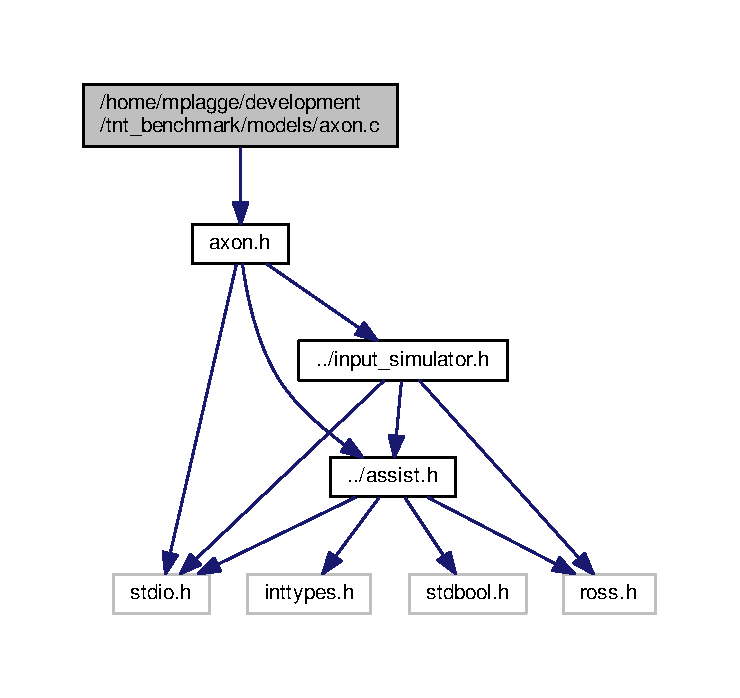
\includegraphics[width=350pt]{axon_8c__incl}
\end{center}
\end{figure}
\subsection*{Functions}
\begin{DoxyCompactItemize}
\item 
void \hyperlink{axon_8c_ab136d88cfbbb1e9f0f3687908dd54851}{axon\+Receive\+Message} (\hyperlink{structaxon_state}{axon\+State} $\ast$st, \hyperlink{struct_msg___data}{Msg\+\_\+\+Data} $\ast$M, tw\+\_\+lp $\ast$lp)
\begin{DoxyCompactList}\small\item\em Handles a message sent to an Axon. \end{DoxyCompactList}\item 
void \hyperlink{axon_8c_a4540abe1d7c57cae5b0ff088d3d47fd1}{axon\+Reverse\+State} (\hyperlink{structaxon_state}{axon\+State} $\ast$st, \hyperlink{struct_msg___data}{Msg\+\_\+\+Data} $\ast$M, tw\+\_\+lp $\ast$lp)
\end{DoxyCompactItemize}


\subsection{Function Documentation}
\hypertarget{axon_8c_ab136d88cfbbb1e9f0f3687908dd54851}{}\index{axon.\+c@{axon.\+c}!axon\+Receive\+Message@{axon\+Receive\+Message}}
\index{axon\+Receive\+Message@{axon\+Receive\+Message}!axon.\+c@{axon.\+c}}
\subsubsection[{axon\+Receive\+Message}]{\setlength{\rightskip}{0pt plus 5cm}void axon\+Receive\+Message (
\begin{DoxyParamCaption}
\item[{{\bf axon\+State} $\ast$}]{st, }
\item[{{\bf Msg\+\_\+\+Data} $\ast$}]{M, }
\item[{tw\+\_\+lp $\ast$}]{lp}
\end{DoxyParamCaption}
)}\label{axon_8c_ab136d88cfbbb1e9f0f3687908dd54851}


Handles a message sent to an Axon. 


\begin{DoxyParams}{Parameters}
{\em st} & state \\
\hline
{\em M} & message \\
\hline
{\em lp} & lp \\
\hline
\end{DoxyParams}


Definition at line \hyperlink{axon_8c_source_l00011}{11} of file \hyperlink{axon_8c_source}{axon.\+c}.



References \hyperlink{assist_8h_source_l00058}{A\+X\+O\+N\+\_\+\+O\+U\+T}, \hyperlink{axon_8h_source_l00018}{axon\+State\+::dest\+Synapse}, \hyperlink{assist_8h_source_l00071}{Msg\+\_\+\+Data\+::event\+Type}, \hyperlink{assist_8c_source_l00014}{get\+Next\+Event\+Time()}, \hyperlink{assist_8h_source_l00061}{N\+E\+U\+R\+O\+N\+\_\+\+O\+U\+T}, \hyperlink{assist_8h_source_l00072}{Msg\+\_\+\+Data\+::rnd\+Call\+Count}, and \hyperlink{axon_8h_source_l00017}{axon\+State\+::send\+Msg\+Count}.


\begin{DoxyCode}
00011                                                               \{
00012     \textcolor{keywordtype}{long} start\_count = lp->rng->count;
00013     tw\_stime time;
00014     st->\hyperlink{structaxon_state_a217ba44fb923dc4dc62bb73b14e61517}{sendMsgCount} ++;
00015     \textcolor{keywordflow}{if}(M->\hyperlink{struct_msg___data_a015b6eb45982e1842ee8fc389a099ced}{eventType} == \hyperlink{assist_8h_a7c1688de451e0dea1e11617bce3ec450a777cedd6ca25a5d7a84aab10a8735af0}{NEURON\_OUT}) \{
00016             time = \hyperlink{assist_8c_a30602b11dbfa6bcb90dc00e7942cfb02}{getNextEventTime}(lp);
00017             tw\_event *newEvent = tw\_event\_new(st->\hyperlink{structaxon_state_a665999819b255f36d756f17b85bc9a03}{destSynapse}, time, lp);
00018             \hyperlink{struct_msg___data}{Msg\_Data} *data = (\hyperlink{struct_msg___data}{Msg\_Data} * ) tw\_event\_data(newEvent);
00019             data->\hyperlink{struct_msg___data_a015b6eb45982e1842ee8fc389a099ced}{eventType} = \hyperlink{assist_8h_a7c1688de451e0dea1e11617bce3ec450abb8b28588ca2e1c33d29df003b3b90ee}{AXON\_OUT};
00020             tw\_event\_send(newEvent);
00021     \}
00022     \textcolor{keywordflow}{else} \{
00023             \textcolor{comment}{//Call the signal generator. TBD}
00024 
00025     \}
00026     M->\hyperlink{struct_msg___data_a2e49a6bcc6c45ade722f746b1ea707f2}{rndCallCount} = lp->rng->count - start\_count;
00027 
00028 \}
\end{DoxyCode}


Here is the call graph for this function\+:\nopagebreak
\begin{figure}[H]
\begin{center}
\leavevmode
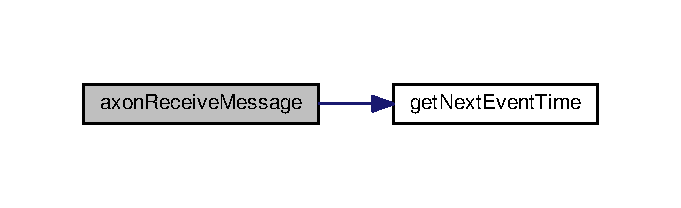
\includegraphics[width=327pt]{axon_8c_ab136d88cfbbb1e9f0f3687908dd54851_cgraph}
\end{center}
\end{figure}


\hypertarget{axon_8c_a4540abe1d7c57cae5b0ff088d3d47fd1}{}\index{axon.\+c@{axon.\+c}!axon\+Reverse\+State@{axon\+Reverse\+State}}
\index{axon\+Reverse\+State@{axon\+Reverse\+State}!axon.\+c@{axon.\+c}}
\subsubsection[{axon\+Reverse\+State}]{\setlength{\rightskip}{0pt plus 5cm}void axon\+Reverse\+State (
\begin{DoxyParamCaption}
\item[{{\bf axon\+State} $\ast$}]{st, }
\item[{{\bf Msg\+\_\+\+Data} $\ast$}]{M, }
\item[{tw\+\_\+lp $\ast$}]{lp}
\end{DoxyParamCaption}
)}\label{axon_8c_a4540abe1d7c57cae5b0ff088d3d47fd1}


Definition at line \hyperlink{axon_8c_source_l00029}{29} of file \hyperlink{axon_8c_source}{axon.\+c}.



References \hyperlink{assist_8h_source_l00072}{Msg\+\_\+\+Data\+::rnd\+Call\+Count}, and \hyperlink{axon_8h_source_l00017}{axon\+State\+::send\+Msg\+Count}.


\begin{DoxyCode}
00029                                                              \{
00030     st->\hyperlink{structaxon_state_a217ba44fb923dc4dc62bb73b14e61517}{sendMsgCount} --;
00031     \textcolor{keywordtype}{long} count = M->\hyperlink{struct_msg___data_a2e49a6bcc6c45ade722f746b1ea707f2}{rndCallCount};
00032     \textcolor{keywordflow}{while} (count--) \{
00033         tw\_rand\_reverse\_unif(lp->rng);
00034     \}
00035 
00036 \}\end{DoxyCode}

\hypertarget{axon_8c_source}{}\section{axon.\+c}
\label{axon_8c_source}\index{/\+Users/\+Mark/\+Development/\+True\+North/tnt\+\_\+benchmark/models/axon.\+c@{/\+Users/\+Mark/\+Development/\+True\+North/tnt\+\_\+benchmark/models/axon.\+c}}

\begin{DoxyCode}
00001 \textcolor{comment}{//}
00002 \textcolor{comment}{//  axon.c}
00003 \textcolor{comment}{//  ROSS\_TOP}
00004 \textcolor{comment}{//}
00005 \textcolor{comment}{//  Created by Mark Plagge on 6/18/15.}
00006 \textcolor{comment}{//}
00007 \textcolor{comment}{//}
00008 
00009 \textcolor{preprocessor}{#}\textcolor{preprocessor}{include} \hyperlink{axon_8h}{"axon.h"}
\end{DoxyCode}

\hypertarget{axon_8h}{}\section{/\+Users/\+Mark/\+Development/\+True\+North/tnt\+\_\+benchmark/models/axon.h File Reference}
\label{axon_8h}\index{/\+Users/\+Mark/\+Development/\+True\+North/tnt\+\_\+benchmark/models/axon.\+h@{/\+Users/\+Mark/\+Development/\+True\+North/tnt\+\_\+benchmark/models/axon.\+h}}
{\ttfamily \#include $<$stdio.\+h$>$}\\*
{\ttfamily \#include \char`\"{}../assist.\+h\char`\"{}}\\*
Include dependency graph for axon.\+h\+:
\nopagebreak
\begin{figure}[H]
\begin{center}
\leavevmode
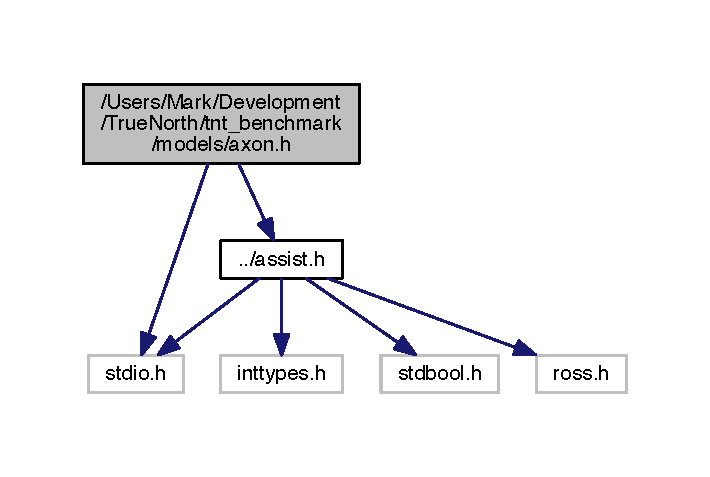
\includegraphics[width=341pt]{axon_8h__incl}
\end{center}
\end{figure}
This graph shows which files directly or indirectly include this file\+:
\nopagebreak
\begin{figure}[H]
\begin{center}
\leavevmode
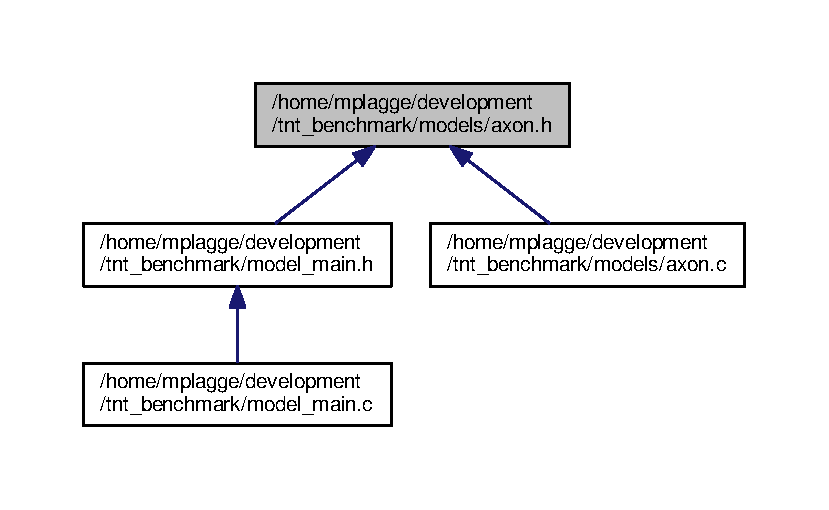
\includegraphics[width=212pt]{axon_8h__dep__incl}
\end{center}
\end{figure}
\subsection*{Data Structures}
\begin{DoxyCompactItemize}
\item 
struct \hyperlink{structaxon_state}{axon\+State}
\end{DoxyCompactItemize}

\hypertarget{axon_8h_source}{}\section{axon.\+h}
\label{axon_8h_source}\index{/home/mplagge/development/tnt\+\_\+benchmark/models/axon.\+h@{/home/mplagge/development/tnt\+\_\+benchmark/models/axon.\+h}}

\begin{DoxyCode}
00001 \textcolor{comment}{//}
00002 \textcolor{comment}{//  axon.h}
00003 \textcolor{comment}{//  ROSS\_TOP}
00004 \textcolor{comment}{//}
00005 \textcolor{comment}{//  Created by Mark Plagge on 6/18/15.}
00006 \textcolor{comment}{//}
00007 \textcolor{comment}{//}
00008 
00009 \textcolor{preprocessor}{#ifndef \_\_ROSS\_TOP\_\_axon\_\_}
00010 \textcolor{preprocessor}{#define \_\_ROSS\_TOP\_\_axon\_\_}
00011 
00012 \textcolor{preprocessor}{#include <stdio.h>}
00013 \textcolor{preprocessor}{#include "../assist.h"}
00014 \textcolor{preprocessor}{#include "../input\_simulator.h"}
00015 
\hypertarget{axon_8h_source_l00016}{}\hyperlink{structaxon_state}{00016} \textcolor{keyword}{typedef} \textcolor{keyword}{struct }AxonState \{
\hypertarget{axon_8h_source_l00017}{}\hyperlink{structaxon_state_a217ba44fb923dc4dc62bb73b14e61517}{00017}     \hyperlink{assist_8h_ad77e6fc5a9b03d46e7c97b7c4b92e89f}{\_statT} \hyperlink{structaxon_state_a217ba44fb923dc4dc62bb73b14e61517}{sendMsgCount};
\hypertarget{axon_8h_source_l00018}{}\hyperlink{structaxon_state_a665999819b255f36d756f17b85bc9a03}{00018}     tw\_lpid \hyperlink{structaxon_state_a665999819b255f36d756f17b85bc9a03}{destSynapse};
00019 
\hypertarget{axon_8h_source_l00020}{}\hyperlink{structaxon_state_ad1d67487729ff78dd3f00885184b1ef3}{00020}     \hyperlink{structinput_simulator_state}{inputSimulatorState} *\hyperlink{structaxon_state_ad1d67487729ff78dd3f00885184b1ef3}{sim};
00021 \}\hyperlink{structaxon_state}{axonState};
00029 \textcolor{keywordtype}{void} \hyperlink{axon_8h_ab136d88cfbbb1e9f0f3687908dd54851}{axonReceiveMessage}(\hyperlink{structaxon_state}{axonState} *st, \hyperlink{struct_msg___data}{Msg\_Data} *M, tw\_lp *lp);
00030 \textcolor{keywordtype}{void} \hyperlink{axon_8h_a4540abe1d7c57cae5b0ff088d3d47fd1}{axonReverseState}(\hyperlink{structaxon_state}{axonState} *st, \hyperlink{struct_msg___data}{Msg\_Data} *M, tw\_lp *lp);
00031 \textcolor{preprocessor}{#endif }\textcolor{comment}{/* defined(\_\_ROSS\_TOP\_\_axon\_\_) */}\textcolor{preprocessor}{}
\end{DoxyCode}

\hypertarget{neuron_8c}{}\section{/\+Users/\+Mark/\+Development/\+True\+North/tnt\+\_\+benchmark/models/neuron.c File Reference}
\label{neuron_8c}\index{/\+Users/\+Mark/\+Development/\+True\+North/tnt\+\_\+benchmark/models/neuron.\+c@{/\+Users/\+Mark/\+Development/\+True\+North/tnt\+\_\+benchmark/models/neuron.\+c}}
{\ttfamily \#include \char`\"{}neuron.\+h\char`\"{}}\\*
Include dependency graph for neuron.\+c\+:
\nopagebreak
\begin{figure}[H]
\begin{center}
\leavevmode
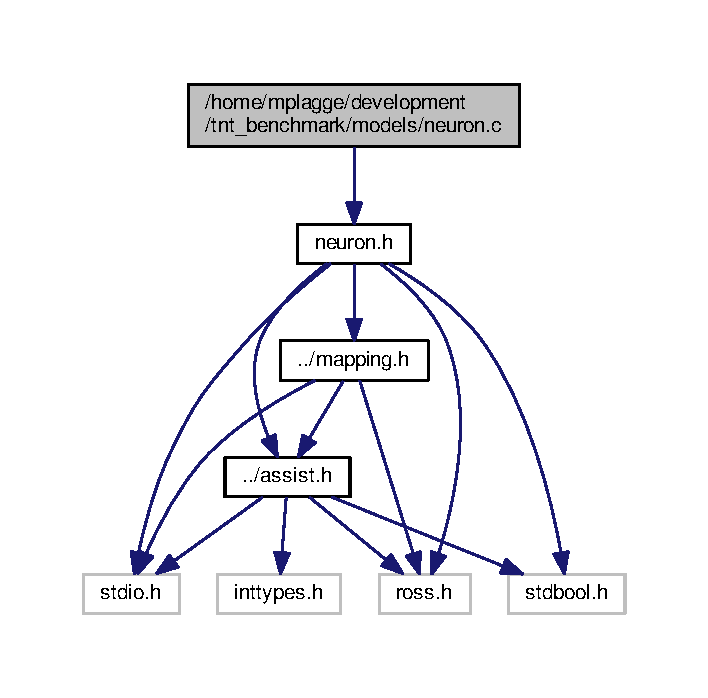
\includegraphics[width=338pt]{neuron_8c__incl}
\end{center}
\end{figure}

\hypertarget{neuron_8c_source}{}\section{neuron.\+c}
\label{neuron_8c_source}\index{/\+Users/\+Mark/\+Development/\+True\+North/tnt\+\_\+benchmark/models/neuron.\+c@{/\+Users/\+Mark/\+Development/\+True\+North/tnt\+\_\+benchmark/models/neuron.\+c}}

\begin{DoxyCode}
00001 \textcolor{comment}{//}
00002 \textcolor{comment}{//  neuron.c}
00003 \textcolor{comment}{//  ROSS\_TOP}
00004 \textcolor{comment}{//}
00005 \textcolor{comment}{//  Created by Mark Plagge on 6/18/15.}
00006 \textcolor{comment}{//}
00007 \textcolor{comment}{//}
00008 
00009 \textcolor{preprocessor}{#}\textcolor{preprocessor}{include} \hyperlink{neuron_8h}{"neuron.h"}
00010 
00011 \textcolor{comment}{/** @name LeakFunctions}
00012 \textcolor{comment}{ * Neuron functions that manage leaks. All voltage state saving}
00013 \textcolor{comment}{ * must be handled in the neuron event function neuronReceiveMessage().}
00014 \textcolor{comment}{ * @\{}
00015 \textcolor{comment}{ */}
\hypertarget{neuron_8c_source_l00016}{}\hyperlink{neuron_8h_a8e52befc10f975c6be39cc93af573d7e}{00016} \textcolor{keywordtype}{void} \hyperlink{neuron_8h_a8e52befc10f975c6be39cc93af573d7e}{noLeak}(\textcolor{keywordtype}{void} *neuron, tw\_stime now) \{
00017   \textcolor{comment}{// do nothing!!}
00018 \}
\hypertarget{neuron_8c_source_l00019}{}\hyperlink{neuron_8h_ac5bebec77c5216533ec5f6acd086532e}{00019} \textcolor{keywordtype}{void} \hyperlink{neuron_8h_ac5bebec77c5216533ec5f6acd086532e}{revNoLeak}(\textcolor{keywordtype}{void} *neuron, tw\_stime now) \{
00020   \textcolor{comment}{// do nothing!!}
00021 \}
00022 \textcolor{comment}{/**}
00023 \textcolor{comment}{ *  @details LinearLeak is the standard linear leak function from the paper. Using the leakRate
       parameter inside \(\backslash\)link NeuronModel the neuron state \(\backslash\)endlink, this follows a simple linear function, reducing the
       membrane potential by a fixed rate per tick.}
00024 \textcolor{comment}{ *}
00025 \textcolor{comment}{}
00026 \textcolor{comment}{ *  @see NeuronModel}
00027 \textcolor{comment}{ */}
\hypertarget{neuron_8c_source_l00028}{}\hyperlink{neuron_8h_a64dc379b459a2b07b40bce35381210e8}{00028} \textcolor{keywordtype}{void} \hyperlink{neuron_8h_a64dc379b459a2b07b40bce35381210e8}{linearLeak}(\textcolor{keywordtype}{void} *neuron, tw\_stime now) \{
00029     neuronState *s = (neuronState *)neuron;
00030     tw\_stime bigTick = getCurrentBigTick(now);
00031     tw\_stime delta = bigTick - s->lastLeakTime;
00032 
00033     s->membranePot -= s->leakRate * delta;
00034     s->lastLeakTime = now;
00035 \}
00036 
\hypertarget{neuron_8c_source_l00037}{}\hyperlink{neuron_8h_a26ced40d7ad7a0b448a136d8724fe18b}{00037} \textcolor{keywordtype}{void} \hyperlink{neuron_8h_a26ced40d7ad7a0b448a136d8724fe18b}{revLinearLeak}(\textcolor{keywordtype}{void} *neuron, tw\_stime now)\{
00038     neuronState *s = (neuronState *)neuron;
00039     tw\_stime delta = s->lastLeakTime - now;
00040 
00041     s->membranePot += s->leakRate * delta;
00042     s->lastLeakTime = now;
00043 \}
00044 
00045 
00046 
00047 \textcolor{comment}{/** @\}*/}
00048 \textcolor{comment}{/** @name ResetFunctions  }
00049 \textcolor{comment}{ Reset function defs. Neuron reset functions will}
00050 \textcolor{comment}{ change the neuron state without saving the previous state. All voltage state saving}
00051 \textcolor{comment}{ must be handled in the neuron event function neuronReceiveMessage(). }
00052 \textcolor{comment}{ @todo: Check that reverse reset functions are needed, since previous voltage is stored in the neuron.}
00053 \textcolor{comment}{ * @\{ */}
00054 
00055 
\hypertarget{neuron_8c_source_l00056}{}\hyperlink{neuron_8h_a7f8eaa35f03747c795a2b727b364537b}{00056} \textcolor{keywordtype}{void} \hyperlink{neuron_8h_a7f8eaa35f03747c795a2b727b364537b}{resetZero}(\textcolor{keywordtype}{void} *neuronState) \{
00057     \textcolor{keyword}{struct} \hyperlink{structneuron_state}{NeuronModel} *s = (\textcolor{keyword}{struct} \hyperlink{structneuron_state}{NeuronModel} *)neuronState;
00058     s\hyperlink{structneuron_state_a0fdd8f44c4105a94e17c4c58a51db486}{->}\hyperlink{structneuron_state_a0fdd8f44c4105a94e17c4c58a51db486}{membranePot} = 0; \textcolor{comment}{// set current voltage to 0.}
00059 \}
00060 
00061 \textcolor{comment}{/**}
00062 \textcolor{comment}{ *  @details  Note: Linear functions use the \(\backslash\)link \_voltT voltT \(\backslash\)endlink data type.}
00063 \textcolor{comment}{ *  If a neuron uses a linear reset, this parameter must be set upon neuron creation. }
00064 \textcolor{comment}{ @todo: Check implementation against paper.}
00065 \textcolor{comment}{ *}
00066 \textcolor{comment}{ */}
\hypertarget{neuron_8c_source_l00067}{}\hyperlink{neuron_8h_a2e78d7d2b70bf7349c3854b3727dcc25}{00067} \textcolor{keywordtype}{void} \hyperlink{neuron_8h_a2e78d7d2b70bf7349c3854b3727dcc25}{resetLinear}(\textcolor{keywordtype}{void} *neuronState) \{
00068     \textcolor{keyword}{struct} \hyperlink{structneuron_state}{NeuronModel} *s = (\textcolor{keyword}{struct} \hyperlink{structneuron_state}{NeuronModel} *)neuronState;
00069   \textcolor{comment}{// reduce the value of the neuron based on the linear reduction function}
00070   \textcolor{comment}{// in the paper}
00071     \hyperlink{assist_8h_abe1fc1b8f9efd1187e564bcb8de7f815}{\_voltT} resetParam = (\hyperlink{assist_8h_abe1fc1b8f9efd1187e564bcb8de7f815}{\_voltT}) &resetParam;
00072   s\hyperlink{structneuron_state_a0fdd8f44c4105a94e17c4c58a51db486}{->}\hyperlink{structneuron_state_a0fdd8f44c4105a94e17c4c58a51db486}{membranePot} = s\hyperlink{structneuron_state_a0fdd8f44c4105a94e17c4c58a51db486}{->}\hyperlink{structneuron_state_a0fdd8f44c4105a94e17c4c58a51db486}{membranePot} - resetParam;
00073 \}
00074 
\hypertarget{neuron_8c_source_l00075}{}\hyperlink{neuron_8h_a09e54832158e2f6abe898437979aae00}{00075} \textcolor{keywordtype}{void} \hyperlink{neuron_8h_a09e54832158e2f6abe898437979aae00}{reverseResetLinear}(\textcolor{keywordtype}{void} *neuronState)\{
00076     \textcolor{keyword}{struct} \hyperlink{structneuron_state}{NeuronModel} *s = (\textcolor{keyword}{struct} \hyperlink{structneuron_state}{NeuronModel} *)neuronState;
00077     \hyperlink{assist_8h_abe1fc1b8f9efd1187e564bcb8de7f815}{\_voltT} resetParam = (\hyperlink{assist_8h_abe1fc1b8f9efd1187e564bcb8de7f815}{\_voltT}) &resetParam;
00078     s\hyperlink{structneuron_state_a0fdd8f44c4105a94e17c4c58a51db486}{->}\hyperlink{structneuron_state_a0fdd8f44c4105a94e17c4c58a51db486}{membranePot} = s\hyperlink{structneuron_state_a0fdd8f44c4105a94e17c4c58a51db486}{->}\hyperlink{structneuron_state_a0fdd8f44c4105a94e17c4c58a51db486}{membranePot} + resetParam;
00079 \}
00080 \textcolor{comment}{/** @todo: Check that this is the proper way to handle reset zero function */}
\hypertarget{neuron_8c_source_l00081}{}\hyperlink{neuron_8h_ae53276ccdb759ba1ea09806cbf9fc940}{00081} \textcolor{keywordtype}{void} \hyperlink{neuron_8h_ae53276ccdb759ba1ea09806cbf9fc940}{reverseResetZero}(\textcolor{keywordtype}{void} *neuronState)\{
00082 
00083 \}
00084 
00085 
00086     \textcolor{comment}{/** @\} */}
00087 
00088 \textcolor{comment}{/** @name NeuronFunctions }
00089 \textcolor{comment}{* Main neuron functions and behaviors}
00090 \textcolor{comment}{*  @\{ }
00091 \textcolor{comment}{ */}
00092 
00093 \textcolor{comment}{/**}
00094 \textcolor{comment}{ *  @details  neruonReceiveMessage runs when an event is received by a neuron.}
00095 \textcolor{comment}{ *  The events are handled in the following fashion:}
00096 \textcolor{comment}{ *  - If the event is a synapse, the neuron integrates the weight of the synapse into its membrane
       potential.}
00097 \textcolor{comment}{ *    - The count of big-tick synapse messages recived is incremented.}
00098 \textcolor{comment}{ *    - If the count changes from zero to one, the function creates and queues a heartbeat event for
       the next big-tick.}
00099 \textcolor{comment}{ *  - If the event is a heartbeat, the neuron will leak, potentially fire, and reset.}
00100 \textcolor{comment}{ *}
00101 \textcolor{comment}{ *  Big-Tick events are sent at time \(\backslash\)f$𝒯\_\{bigTick\} - ε\(\backslash\)f$, so that the the event will arrive at the
       next bit-tick time.}
00102 \textcolor{comment}{ *}
00103 \textcolor{comment}{ */}
\hypertarget{neuron_8c_source_l00104}{}\hyperlink{neuron_8h_aa6819d7492f0173f2234ba0b8b0bb674}{00104} \textcolor{keywordtype}{void} \hyperlink{neuron_8h_aa6819d7492f0173f2234ba0b8b0bb674}{neuronReceiveMessage}(neuronState *st, tw\_stime time, Msg\_Data *m,
00105 tw\_lp *lp)\{
00106     \textcolor{keywordtype}{bool} willFire = \textcolor{keyword}{false};
00107         \textcolor{comment}{//save the previous state of the neuron:}
00108     st->savedLastLeakTime = st->lastLeakTime;
00109     st->savedLastActiveTime = st->lastActiveTime;
00110     st\hyperlink{structneuron_state_a5efe5de0478ea513ed5d90d89a49fcca}{->}\hyperlink{structneuron_state_a5efe5de0478ea513ed5d90d89a49fcca}{savedMembranePot} = st\hyperlink{structneuron_state_a0fdd8f44c4105a94e17c4c58a51db486}{->}\hyperlink{structneuron_state_a0fdd8f44c4105a94e17c4c58a51db486}{membranePot};
00111         \textcolor{comment}{//random fn call state management.}
00112     \textcolor{keywordtype}{unsigned} \textcolor{keywordtype}{long} startCount = lp->rng->count;
00113 
00114     \textcolor{keywordflow}{switch} (m\hyperlink{struct_msg___data_a015b6eb45982e1842ee8fc389a099ced}{->}\hyperlink{struct_msg___data_a015b6eb45982e1842ee8fc389a099ced}{eventType}) \{
00115   \textcolor{keywordflow}{case} SYNAPSE\_OUT:
00116             integrateSynapse(m->localID, st, lp);
00117 
00118                 \textcolor{comment}{//next, we will check if a heartbeat message should be sent}
00119             \textcolor{keywordflow}{if}(st\hyperlink{structneuron_state_af8935bcba177f2f3dfb9119c39ef7dc5}{->}\hyperlink{structneuron_state_af8935bcba177f2f3dfb9119c39ef7dc5}{receivedSynapseMsgs} == 0) \{
00120                 sendHeartbeat(st, lp, time);
00121             \}
00122             st\hyperlink{structneuron_state_af8935bcba177f2f3dfb9119c39ef7dc5}{->}\hyperlink{structneuron_state_af8935bcba177f2f3dfb9119c39ef7dc5}{receivedSynapseMsgs} ++;
00123 
00124 
00125             \textcolor{keywordflow}{break};
00126 
00127         \textcolor{keywordflow}{case} \hyperlink{assist_8h_a7c1688de451e0dea1e11617bce3ec450a226690009a653238a52339561e6c466e}{NEURON\_HEARTBEAT}:
00128             st\hyperlink{structneuron_state_af8935bcba177f2f3dfb9119c39ef7dc5}{->}\hyperlink{structneuron_state_af8935bcba177f2f3dfb9119c39ef7dc5}{receivedSynapseMsgs} = 0;
00129 
00130                 \textcolor{comment}{//Currently operates - leak->fire->(reset)}
00131             st->doLeak(st, time);
00132             willFire = \hyperlink{neuron_8h_a92d5882a15e11e2a6733483d51428e46}{neuronShouldFire}\hyperlink{neuron_8h_a92d5882a15e11e2a6733483d51428e46}{(}st\hyperlink{neuron_8h_a92d5882a15e11e2a6733483d51428e46}{)};
00133             \textcolor{keywordflow}{if}(willFire)\{
00134                 neuronFire(st, time, m);
00135                 neuronPostFire(st, time, m);
00136                 st\hyperlink{structneuron_state_afe8825076c4cf3863c677307fec63c61}{->}\hyperlink{structneuron_state_afe8825076c4cf3863c677307fec63c61}{fireCount} ++;
00137             \}
00138 
00139             neuronPostIntegrate(st, time, lp, willFire);
00140             \textcolor{comment}{//stats collection}
00141             st\hyperlink{structneuron_state_a71fbb9a79e8048b473b6e09d29a64bbe}{->}\hyperlink{structneuron_state_a71fbb9a79e8048b473b6e09d29a64bbe}{SOPSCount} ++;
00142             \textcolor{keywordflow}{break};
00143 
00144   \textcolor{keywordflow}{default}:
00145                 \textcolor{comment}{//Error condition - non-valid input.}
00146             \textcolor{keywordflow}{break};
00147     \}
00148 
00149         \textcolor{comment}{//store the random calls in the message:}
00150     m->rndCallCount = lp->rng->count - startCount;
00151 
00152     st\hyperlink{structneuron_state_ab8f63a1dfdb2992657530ff8a63fdc01}{->}\hyperlink{structneuron_state_ab8f63a1dfdb2992657530ff8a63fdc01}{rcvdMsgCount} ++;
00153 
00154 
00155 
00156 \}
\hypertarget{neuron_8c_source_l00157}{}\hyperlink{neuron_8h_a92d5882a15e11e2a6733483d51428e46}{00157} \textcolor{keywordtype}{bool} \hyperlink{neuron_8h_a92d5882a15e11e2a6733483d51428e46}{neuronShouldFire}(neuronState *st)\{
00158         \textcolor{comment}{//check negative threshold values:}
00159     \textcolor{keywordflow}{if}(st->membranePot < ) \{
00160         \textcolor{keywordflow}{if}(st->negThresReset) \{
00161                 \textcolor{comment}{//reset to \(\backslash\)f$-β\_j\(\backslash\)f$}
00162         \}
00163     \}
00164     \textcolor{keywordflow}{return} st\hyperlink{structneuron_state_a0fdd8f44c4105a94e17c4c58a51db486}{->}\hyperlink{structneuron_state_a0fdd8f44c4105a94e17c4c58a51db486}{membranePot} > st\hyperlink{structneuron_state_a132470c4c17828c209e3403ccf7ee680}{->}\hyperlink{structneuron_state_a132470c4c17828c209e3403ccf7ee680}{threshold};
00165 \}
\hypertarget{neuron_8c_source_l00166}{}\hyperlink{neuron_8h_ae071ef984b7e0dd4ec38fca91e0abe39}{00166} \textcolor{keywordtype}{void} \hyperlink{neuron_8h_ae071ef984b7e0dd4ec38fca91e0abe39}{neuronFire}(neuronState *st, tw\_stime time, Msg\_Data *m)\{
00167 
00168 \}
\hypertarget{neuron_8c_source_l00169}{}\hyperlink{neuron_8h_ab1f4997e4bfe11e78faa6d37748aee67}{00169} \textcolor{keywordtype}{void} \hyperlink{neuron_8h_ab1f4997e4bfe11e78faa6d37748aee67}{neuronPostFire}(neuronState *st, tw\_stime time, Msg\_Data *m)\{
00170 
00171 \}
\hypertarget{neuron_8c_source_l00172}{}\hyperlink{neuron_8h_a06ee765bfae45fe9b7f0619bf4abe63d}{00172} \textcolor{keywordtype}{void} \hyperlink{neuron_8h_a06ee765bfae45fe9b7f0619bf4abe63d}{generateWaitEvent}(neuronState *st, tw\_stime time, tw\_lp *lp)\{
00173 
00174 \}
\hypertarget{neuron_8c_source_l00175}{}\hyperlink{neuron_8h_ae630bdf5dd3744870968f07a6971659c}{00175} \textcolor{keywordtype}{void} \hyperlink{neuron_8h_ae630bdf5dd3744870968f07a6971659c}{integrateSynapse}(\hyperlink{assist_8h_a3f7a6e6a1210b6d9d7a42177dcb9634b}{\_idT} synapseID,neuronState *st, tw\_lp *lp) \{
00176     \hyperlink{assist_8h_abe1fc1b8f9efd1187e564bcb8de7f815}{\_voltT} adjustedWeight;
00177     \textcolor{keywordflow}{if}(st->perSynapseDet[synapseID] == \textcolor{keyword}{true}) \{
00178         adjustedWeight = st->perSynapseWeight[synapseID];
00179         st->membranePot += adjustedWeight;
00180     \} \textcolor{keywordflow}{else} \{ \textcolor{comment}{//stochastic mode weights:}
00181         \hyperlink{assist_8h_abe1fc1b8f9efd1187e564bcb8de7f815}{\_voltT} rand = tw\_rand\_integer(lp->rng, st->, <#\textcolor{keywordtype}{long} high#>)
00182 
00183 \}
00184 
00185 \textcolor{keywordtype}{void} neuronPostIntegrate(neuronState *st, tw\_stime time, tw\_lp *lp, \textcolor{keywordtype}{bool} didFire)\{
00186 
00187 \}
00188 \textcolor{comment}{/** @\} */}
\end{DoxyCode}

\hypertarget{neuron_8h}{}\section{/home/mplagge/development/tnt\+\_\+benchmark/models/neuron.h File Reference}
\label{neuron_8h}\index{/home/mplagge/development/tnt\+\_\+benchmark/models/neuron.\+h@{/home/mplagge/development/tnt\+\_\+benchmark/models/neuron.\+h}}
{\ttfamily \#include $<$stdio.\+h$>$}\\*
{\ttfamily \#include \char`\"{}../assist.\+h\char`\"{}}\\*
{\ttfamily \#include \char`\"{}../mapping.\+h\char`\"{}}\\*
{\ttfamily \#include \char`\"{}ross.\+h\char`\"{}}\\*
{\ttfamily \#include $<$stdbool.\+h$>$}\\*
Include dependency graph for neuron.\+h\+:\nopagebreak
\begin{figure}[H]
\begin{center}
\leavevmode
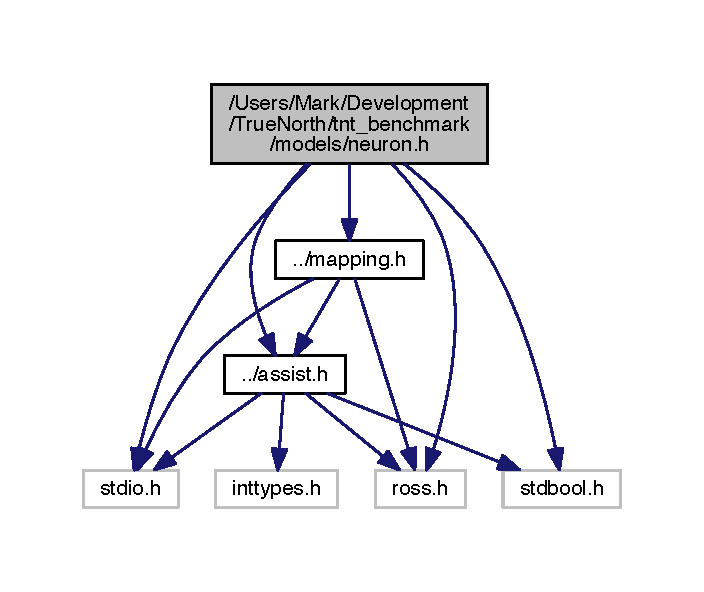
\includegraphics[width=340pt]{neuron_8h__incl}
\end{center}
\end{figure}
This graph shows which files directly or indirectly include this file\+:\nopagebreak
\begin{figure}[H]
\begin{center}
\leavevmode
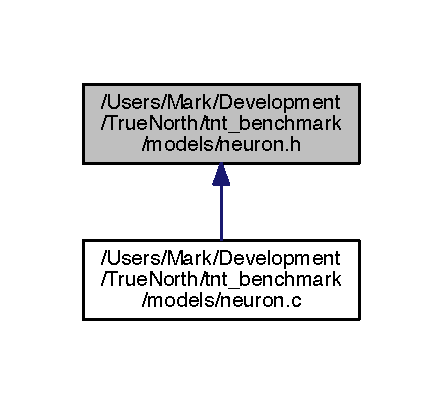
\includegraphics[width=350pt]{neuron_8h__dep__incl}
\end{center}
\end{figure}
\subsection*{Data Structures}
\begin{DoxyCompactItemize}
\item 
union \hyperlink{unionreset_rate}{reset\+Rate}
\begin{DoxyCompactList}\small\item\em Reset\+Rate This is a support union for neuron reset rates. \end{DoxyCompactList}\item 
struct \hyperlink{structneuron_state}{neuron\+State}
\begin{DoxyCompactList}\small\item\em This struct maintains the state of an individual neuron.\+The neuron struct contains the parameters needed to maintain state in the neuron, along with references to output commands (dendrites). \end{DoxyCompactList}\end{DoxyCompactItemize}
\subsection*{Typedefs}
\begin{DoxyCompactItemize}
\item 
typedef void($\ast$ \hyperlink{neuron_8h_a7362d32c8d9b6dc323f5d1b05af9855b}{leak\+Fun\+Del}) (void $\ast$\hyperlink{structneuron_state}{neuron\+State}, tw\+\_\+stime now)
\item 
typedef void($\ast$ \hyperlink{neuron_8h_abf61b10b4b6116161a9e5c9d7ac54be1}{reverse\+Leak\+Del}) (void $\ast$neuron, tw\+\_\+stime now)
\item 
typedef void($\ast$ \hyperlink{neuron_8h_ae7e5990745cd949246894bfb633ca4a2}{reset\+Fun\+Del}) (void $\ast$\hyperlink{structneuron_state}{neuron\+State})
\begin{DoxyCompactList}\small\item\em Reset\+Fun\+Del -\/ This is a function that handles different reset rate calculations. \end{DoxyCompactList}\item 
typedef void($\ast$ \hyperlink{neuron_8h_aa939c0acc5b3367975f2f0cb7bc36d17}{reverse\+Reset\+Del}) (void $\ast$\hyperlink{structneuron_state}{neuron\+State})
\begin{DoxyCompactList}\small\item\em This is a function that reverses the reset command. \end{DoxyCompactList}\end{DoxyCompactItemize}
\subsection*{Enumerations}
\begin{DoxyCompactItemize}
\item 
enum \hyperlink{neuron_8h_a48885ea6be5b55a2e24de9f97552d4ee}{neuron\+Fire\+Mode} \{ \hyperlink{neuron_8h_a48885ea6be5b55a2e24de9f97552d4eea520c6b216334b8c2d914cf9fab8cd460}{N\+F\+M} = 0
 \}
\begin{DoxyCompactList}\small\item\em typedef Neuron\+Fire\+Mode Just in case there are multiple fire modes, this enum exists to differentiate them. \end{DoxyCompactList}\end{DoxyCompactItemize}
\subsection*{Functions}
\begin{DoxyCompactItemize}
\item 
void \hyperlink{neuron_8h_a8e52befc10f975c6be39cc93af573d7e}{no\+Leak} (void $\ast$neuron, tw\+\_\+stime now)
\begin{DoxyCompactList}\small\item\em no\+Leak -\/ A non leaking neuron function. \end{DoxyCompactList}\item 
void \hyperlink{neuron_8h_a64dc379b459a2b07b40bce35381210e8}{linear\+Leak} (void $\ast$neuron, tw\+\_\+stime now)
\begin{DoxyCompactList}\small\item\em A linear leak function -\/ uses monotonic up and down leaks. \end{DoxyCompactList}\item 
void \hyperlink{neuron_8h_a5a4f7abf694fe6ff2aa68ebd5584bc4b}{monotonic\+Up\+Leak} (void $\ast$neuron, tw\+\_\+stime now)
\item 
void \hyperlink{neuron_8h_a8c023bc2fc6d628a105b460226b106f9}{monotonic\+Down\+Leak} (void $\ast$neuron, tw\+\_\+stime now)
\item 
void \hyperlink{neuron_8h_a5477909af0c953cabd578adf0695e5e5}{divergent\+Leak} (void $\ast$neuron, tw\+\_\+stime now)
\item 
void \hyperlink{neuron_8h_ad5df8be6cabf9a00abf073cee3be0362}{convergent\+Leak} (void $\ast$neuron, tw\+\_\+stime now)
\item 
void \hyperlink{neuron_8h_ac5bebec77c5216533ec5f6acd086532e}{rev\+No\+Leak} (void $\ast$neuron, tw\+\_\+stime now)
\begin{DoxyCompactList}\small\item\em Reverse leak function for use when neurons have no defined leak function. \end{DoxyCompactList}\item 
void \hyperlink{neuron_8h_a26ced40d7ad7a0b448a136d8724fe18b}{rev\+Linear\+Leak} (void $\ast$neuron, tw\+\_\+stime now)
\begin{DoxyCompactList}\small\item\em Reverse leak function neurons that have a linear leak function assigned. \end{DoxyCompactList}\item 
void \hyperlink{neuron_8h_a233aa7ebe6cbfb664fe366a05a8dac1f}{reset\+Normal} (void $\ast$\hyperlink{structneuron_state}{neuron\+State})
\begin{DoxyCompactList}\small\item\em Resets neuron voltage to $R$ after firing. \end{DoxyCompactList}\item 
void \hyperlink{neuron_8h_a2e78d7d2b70bf7349c3854b3727dcc25}{reset\+Linear} (void $\ast$\hyperlink{structneuron_state}{neuron\+State})
\begin{DoxyCompactList}\small\item\em Resets neuron voltage based on linear function. \end{DoxyCompactList}\item 
void \hyperlink{neuron_8h_a6e11be912b4860cd1978b2d8c49b9703}{reset\+None} (void $\ast$\hyperlink{structneuron_state}{neuron\+State})
\begin{DoxyCompactList}\small\item\em No reset function -\/ does not reset membrane potential after firing. \end{DoxyCompactList}\item 
void \hyperlink{neuron_8h_a09e54832158e2f6abe898437979aae00}{reverse\+Reset\+Linear} (void $\ast$\hyperlink{structneuron_state}{neuron\+State})
\item 
void \hyperlink{neuron_8h_ae53276ccdb759ba1ea09806cbf9fc940}{reverse\+Reset\+Zero} (void $\ast$\hyperlink{structneuron_state}{neuron\+State})
\item 
void \hyperlink{neuron_8h_a50b2475c0a8d745eb8f144b72d7eabdf}{reverse\+Reset\+None} (void $\ast$\hyperlink{structneuron_state}{neuron\+State})
\item 
void \hyperlink{neuron_8h_a01dcc8e3f0132786bd59ecb847013284}{neuron\+Reverse\+Final} (\hyperlink{structneuron_state}{neuron\+State} $\ast$s, tw\+\_\+bf $\ast$C\+V, \hyperlink{struct_msg___data}{Msg\+\_\+\+Data} $\ast$m, tw\+\_\+lp $\ast$lp)
\begin{DoxyCompactList}\small\item\em neuron\+Reverse\+Final final neuron reversal function. \end{DoxyCompactList}\item 
void \hyperlink{neuron_8h_aa6819d7492f0173f2234ba0b8b0bb674}{neuron\+Receive\+Message} (\hyperlink{structneuron_state}{neuron\+State} $\ast$st, tw\+\_\+stime time, \hyperlink{struct_msg___data}{Msg\+\_\+\+Data} $\ast$m, tw\+\_\+lp $\ast$lp)
\begin{DoxyCompactList}\small\item\em handles incomming synapse messages. \end{DoxyCompactList}\item 
void \hyperlink{neuron_8h_a683379b633b55058dd5b8b67929c165c}{neuron\+Fire} (\hyperlink{structneuron_state}{neuron\+State} $\ast$st, tw\+\_\+stime time, tw\+\_\+lp $\ast$lp)
\begin{DoxyCompactList}\small\item\em neuron\+Fire manages a firing event. \end{DoxyCompactList}\item 
void \hyperlink{neuron_8h_ae630bdf5dd3744870968f07a6971659c}{integrate\+Synapse} (\hyperlink{assist_8h_a3f7a6e6a1210b6d9d7a42177dcb9634b}{\+\_\+id\+T} synapse\+I\+D, \hyperlink{structneuron_state}{neuron\+State} $\ast$st, tw\+\_\+lp $\ast$lp)
\begin{DoxyCompactList}\small\item\em function that adds a synapse\textquotesingle{}s value to the current neuron\textquotesingle{}s membrane potential. \end{DoxyCompactList}\item 
void \hyperlink{neuron_8h_a766dff9e530486b055e97ebe392268b8}{send\+Heartbeat} (\hyperlink{structneuron_state}{neuron\+State} $\ast$st, tw\+\_\+lp $\ast$lp, tw\+\_\+stime time)
\begin{DoxyCompactList}\small\item\em Function that sends a heartbeat message to this neuron. \end{DoxyCompactList}\item 
bool \hyperlink{neuron_8h_a3520b013e0c2f711b9f5c16e19306be6}{neuron\+Should\+Fire} (\hyperlink{structneuron_state}{neuron\+State} $\ast$st, tw\+\_\+lp $\ast$lp)
\begin{DoxyCompactList}\small\item\em Checks to see if a neuron should fire. \end{DoxyCompactList}\item 
void \hyperlink{neuron_8h_aabaff47eadb1e61b34c19b6e982f6511}{neuron\+Post\+Integrate} (\hyperlink{structneuron_state}{neuron\+State} $\ast$st, tw\+\_\+stime time, tw\+\_\+lp $\ast$lp, bool will\+Fire)
\begin{DoxyCompactList}\small\item\em Function that runs after integration \& firing, for reset function and threshold bounce calls. \end{DoxyCompactList}\item 
void \hyperlink{neuron_8h_afee2e0acc66d8d10aee8d52c8d245c82}{stochastic\+Integrate} (\hyperlink{assist_8h_aa73c5ea0fe4ba938c96e6771b38dcb2a}{\+\_\+weight\+T} weight, \hyperlink{structneuron_state}{neuron\+State} $\ast$st, tw\+\_\+lp $\ast$lp)
\begin{DoxyCompactList}\small\item\em Neuron stochastic integration function -\/ for use with stochastic leaks and synapse messages. \end{DoxyCompactList}\item 
void \hyperlink{neuron_8h_aaae24f12a4b2a537740f29d65eb3e51e}{neron\+Reverse\+Sate} (\hyperlink{structneuron_state}{neuron\+State} $\ast$s, tw\+\_\+bf $\ast$C\+V, \hyperlink{struct_msg___data}{Msg\+\_\+\+Data} $\ast$M, tw\+\_\+lp $\ast$lp)
\end{DoxyCompactItemize}


\subsection{Typedef Documentation}
\hypertarget{neuron_8h_a7362d32c8d9b6dc323f5d1b05af9855b}{}\index{neuron.\+h@{neuron.\+h}!leak\+Fun\+Del@{leak\+Fun\+Del}}
\index{leak\+Fun\+Del@{leak\+Fun\+Del}!neuron.\+h@{neuron.\+h}}
\subsubsection[{leak\+Fun\+Del}]{\setlength{\rightskip}{0pt plus 5cm}typedef void($\ast$ {\bf leak\+Fun\+Del}) (void $\ast${\bf neuron\+State}, tw\+\_\+stime now)}\label{neuron_8h_a7362d32c8d9b6dc323f5d1b05af9855b}


Definition at line \hyperlink{neuron_8h_source_l00033}{33} of file \hyperlink{neuron_8h_source}{neuron.\+h}.

\hypertarget{neuron_8h_ae7e5990745cd949246894bfb633ca4a2}{}\index{neuron.\+h@{neuron.\+h}!reset\+Fun\+Del@{reset\+Fun\+Del}}
\index{reset\+Fun\+Del@{reset\+Fun\+Del}!neuron.\+h@{neuron.\+h}}
\subsubsection[{reset\+Fun\+Del}]{\setlength{\rightskip}{0pt plus 5cm}typedef void($\ast$ reset\+Fun\+Del) (void $\ast${\bf neuron\+State})}\label{neuron_8h_ae7e5990745cd949246894bfb633ca4a2}


Reset\+Fun\+Del -\/ This is a function that handles different reset rate calculations. 

It takes the state of the neuron, and applies various reset functions to the neuron\textquotesingle{}s voltage. Some reset functions described by true north include a zeroing function (standard integrate and fire), a linear drop function, and a non-\/reduction function. Also functions for leaks below. 

Definition at line \hyperlink{neuron_8h_source_l00094}{94} of file \hyperlink{neuron_8h_source}{neuron.\+h}.

\hypertarget{neuron_8h_abf61b10b4b6116161a9e5c9d7ac54be1}{}\index{neuron.\+h@{neuron.\+h}!reverse\+Leak\+Del@{reverse\+Leak\+Del}}
\index{reverse\+Leak\+Del@{reverse\+Leak\+Del}!neuron.\+h@{neuron.\+h}}
\subsubsection[{reverse\+Leak\+Del}]{\setlength{\rightskip}{0pt plus 5cm}typedef void($\ast$ {\bf reverse\+Leak\+Del}) (void $\ast$neuron, tw\+\_\+stime now)}\label{neuron_8h_abf61b10b4b6116161a9e5c9d7ac54be1}


Definition at line \hyperlink{neuron_8h_source_l00059}{59} of file \hyperlink{neuron_8h_source}{neuron.\+h}.

\hypertarget{neuron_8h_aa939c0acc5b3367975f2f0cb7bc36d17}{}\index{neuron.\+h@{neuron.\+h}!reverse\+Reset\+Del@{reverse\+Reset\+Del}}
\index{reverse\+Reset\+Del@{reverse\+Reset\+Del}!neuron.\+h@{neuron.\+h}}
\subsubsection[{reverse\+Reset\+Del}]{\setlength{\rightskip}{0pt plus 5cm}reverse\+Reset\+Del}\label{neuron_8h_aa939c0acc5b3367975f2f0cb7bc36d17}


This is a function that reverses the reset command. 

Run first, since the reset function is run last. 

Definition at line \hyperlink{neuron_8h_source_l00125}{125} of file \hyperlink{neuron_8h_source}{neuron.\+h}.



\subsection{Enumeration Type Documentation}
\hypertarget{neuron_8h_a48885ea6be5b55a2e24de9f97552d4ee}{}\index{neuron.\+h@{neuron.\+h}!neuron\+Fire\+Mode@{neuron\+Fire\+Mode}}
\index{neuron\+Fire\+Mode@{neuron\+Fire\+Mode}!neuron.\+h@{neuron.\+h}}
\subsubsection[{neuron\+Fire\+Mode}]{\setlength{\rightskip}{0pt plus 5cm}enum {\bf neuron\+Fire\+Mode}}\label{neuron_8h_a48885ea6be5b55a2e24de9f97552d4ee}


typedef Neuron\+Fire\+Mode Just in case there are multiple fire modes, this enum exists to differentiate them. 

\begin{Desc}
\item[Enumerator]\par
\begin{description}
\index{N\+F\+M@{N\+F\+M}!neuron.\+h@{neuron.\+h}}\index{neuron.\+h@{neuron.\+h}!N\+F\+M@{N\+F\+M}}\item[{\em 
\hypertarget{neuron_8h_a48885ea6be5b55a2e24de9f97552d4eea520c6b216334b8c2d914cf9fab8cd460}{}N\+F\+M\label{neuron_8h_a48885ea6be5b55a2e24de9f97552d4eea520c6b216334b8c2d914cf9fab8cd460}
}]\end{description}
\end{Desc}


Definition at line \hyperlink{neuron_8h_source_l00023}{23} of file \hyperlink{neuron_8h_source}{neuron.\+h}.


\begin{DoxyCode}
00023                                 \{
00024   \hyperlink{neuron_8h_a48885ea6be5b55a2e24de9f97552d4eea520c6b216334b8c2d914cf9fab8cd460}{NFM} = 0  \textcolor{comment}{// normal fire mode (if voltage > threshold, fire);}
00025     \} \hyperlink{neuron_8h_a48885ea6be5b55a2e24de9f97552d4ee}{neuronFireMode};
\end{DoxyCode}


\subsection{Function Documentation}
\hypertarget{neuron_8h_ad5df8be6cabf9a00abf073cee3be0362}{}\index{neuron.\+h@{neuron.\+h}!convergent\+Leak@{convergent\+Leak}}
\index{convergent\+Leak@{convergent\+Leak}!neuron.\+h@{neuron.\+h}}
\subsubsection[{convergent\+Leak}]{\setlength{\rightskip}{0pt plus 5cm}void convergent\+Leak (
\begin{DoxyParamCaption}
\item[{void $\ast$}]{neuron, }
\item[{tw\+\_\+stime}]{now}
\end{DoxyParamCaption}
)}\label{neuron_8h_ad5df8be6cabf9a00abf073cee3be0362}
\hypertarget{neuron_8h_a5477909af0c953cabd578adf0695e5e5}{}\index{neuron.\+h@{neuron.\+h}!divergent\+Leak@{divergent\+Leak}}
\index{divergent\+Leak@{divergent\+Leak}!neuron.\+h@{neuron.\+h}}
\subsubsection[{divergent\+Leak}]{\setlength{\rightskip}{0pt plus 5cm}void divergent\+Leak (
\begin{DoxyParamCaption}
\item[{void $\ast$}]{neuron, }
\item[{tw\+\_\+stime}]{now}
\end{DoxyParamCaption}
)}\label{neuron_8h_a5477909af0c953cabd578adf0695e5e5}
\hypertarget{neuron_8h_ae630bdf5dd3744870968f07a6971659c}{}\index{neuron.\+h@{neuron.\+h}!integrate\+Synapse@{integrate\+Synapse}}
\index{integrate\+Synapse@{integrate\+Synapse}!neuron.\+h@{neuron.\+h}}
\subsubsection[{integrate\+Synapse}]{\setlength{\rightskip}{0pt plus 5cm}void integrate\+Synapse (
\begin{DoxyParamCaption}
\item[{{\bf \+\_\+id\+T}}]{synapse\+I\+D, }
\item[{{\bf neuron\+State} $\ast$}]{st, }
\item[{tw\+\_\+lp $\ast$}]{lp}
\end{DoxyParamCaption}
)}\label{neuron_8h_ae630bdf5dd3744870968f07a6971659c}


function that adds a synapse\textquotesingle{}s value to the current neuron\textquotesingle{}s membrane potential. 


\begin{DoxyParams}{Parameters}
{\em synapse\+I\+D} & local\+I\+D of the synapse sending the message. \\
\hline
\end{DoxyParams}


Definition at line \hyperlink{neuron_8c_source_l00199}{199} of file \hyperlink{neuron_8c_source}{neuron.\+c}.



References \hyperlink{assist_8h_source_l00020}{\+\_\+volt\+T}, \hyperlink{neuron_8h_source_l00153}{neuron\+State\+::membrane\+Pot}, \hyperlink{neuron_8c_source_l00191}{stochastic\+Integrate()}, \hyperlink{neuron_8h_source_l00187}{neuron\+State\+::synaptic\+Weight\+Prob}, and \hyperlink{neuron_8h_source_l00192}{neuron\+State\+::synaptic\+Weight\+Prob\+Select}.



Referenced by \hyperlink{neuron_8c_source_l00103}{neuron\+Receive\+Message()}.


\begin{DoxyCode}
00199                                                                  \{
00200 
00201     \textcolor{keywordflow}{if}(st->\hyperlink{structneuron_state_a4568f103808a436a62d7c7c47dc90e9b}{synapticWeightProbSelect}[synapseID] == \textcolor{keyword}{true}) \{
00202         \hyperlink{neuron_8c_afee2e0acc66d8d10aee8d52c8d245c82}{stochasticIntegrate}(st->\hyperlink{structneuron_state_aa71c0acf1edf08865e1f9729a2414efa}{synapticWeightProb}[synapseID], st, lp)
      ;
00203     \} \textcolor{keywordflow}{else} \{ \textcolor{comment}{//det. mode integrate:}
00204         \hyperlink{assist_8h_abe1fc1b8f9efd1187e564bcb8de7f815}{\_voltT} adjustedWeight = st->\hyperlink{structneuron_state_aa71c0acf1edf08865e1f9729a2414efa}{synapticWeightProb}[synapseID];
00205         st->\hyperlink{structneuron_state_a0fdd8f44c4105a94e17c4c58a51db486}{membranePot} += adjustedWeight;
00206     \}
00207 
00208 
00209 \}
\end{DoxyCode}


Here is the call graph for this function\+:\nopagebreak
\begin{figure}[H]
\begin{center}
\leavevmode
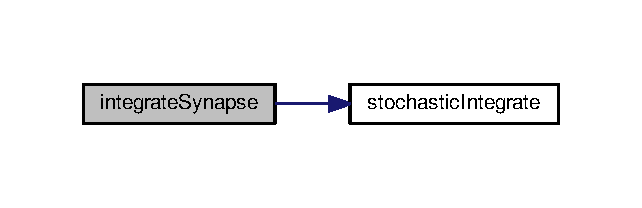
\includegraphics[width=308pt]{neuron_8h_ae630bdf5dd3744870968f07a6971659c_cgraph}
\end{center}
\end{figure}


\hypertarget{neuron_8h_a64dc379b459a2b07b40bce35381210e8}{}\index{neuron.\+h@{neuron.\+h}!linear\+Leak@{linear\+Leak}}
\index{linear\+Leak@{linear\+Leak}!neuron.\+h@{neuron.\+h}}
\subsubsection[{linear\+Leak}]{\setlength{\rightskip}{0pt plus 5cm}void linear\+Leak (
\begin{DoxyParamCaption}
\item[{void $\ast$}]{neuron, }
\item[{tw\+\_\+stime}]{now}
\end{DoxyParamCaption}
)}\label{neuron_8h_a64dc379b459a2b07b40bce35381210e8}


A linear leak function -\/ uses monotonic up and down leaks. 


\begin{DoxyParams}{Parameters}
{\em neuron} & The current neuron state. \\
\hline
{\em now} & The current simulation time.\\
\hline
\end{DoxyParams}
Linear\+Leak is the standard linear leak function from the paper. Using the leak\+Rate parameter inside \hyperlink{}{the neuron state }, this follows a simple linear function, reducing the membrane potential by a fixed rate per tick.

\begin{DoxySeeAlso}{See also}
Neuron\+Model 
\end{DoxySeeAlso}


Definition at line \hyperlink{neuron_8c_source_l00028}{28} of file \hyperlink{neuron_8c_source}{neuron.\+c}.



References \hyperlink{assist_8c_source_l00030}{get\+Current\+Big\+Tick()}, and \hyperlink{neuron_8h_source_l00162}{neuron\+State\+::last\+Leak\+Time}.


\begin{DoxyCode}
00028                                             \{
00029     \hyperlink{structneuron_state}{neuronState} *s = (\hyperlink{structneuron_state}{neuronState} *)neuron;
00030     tw\_stime bigTick = \hyperlink{assist_8c_a4d378196b7fceed090d64ec8820b4065}{getCurrentBigTick}(now);
00031     tw\_stime delta = bigTick - s->\hyperlink{structneuron_state_a6f4e4d8fc1cf0257b486e01f628d2656}{lastLeakTime};
00032 
00033         \textcolor{comment}{//s->membranePot -= s->leakRate * delta;}
00034     s->\hyperlink{structneuron_state_a6f4e4d8fc1cf0257b486e01f628d2656}{lastLeakTime} = now;
00035 \}
\end{DoxyCode}


Here is the call graph for this function\+:\nopagebreak
\begin{figure}[H]
\begin{center}
\leavevmode
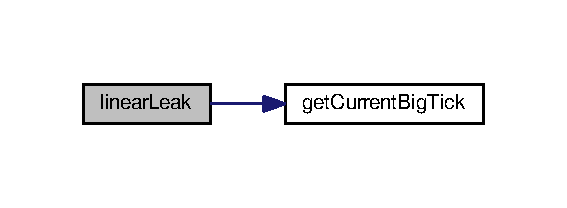
\includegraphics[width=272pt]{neuron_8h_a64dc379b459a2b07b40bce35381210e8_cgraph}
\end{center}
\end{figure}


\hypertarget{neuron_8h_a8c023bc2fc6d628a105b460226b106f9}{}\index{neuron.\+h@{neuron.\+h}!monotonic\+Down\+Leak@{monotonic\+Down\+Leak}}
\index{monotonic\+Down\+Leak@{monotonic\+Down\+Leak}!neuron.\+h@{neuron.\+h}}
\subsubsection[{monotonic\+Down\+Leak}]{\setlength{\rightskip}{0pt plus 5cm}void monotonic\+Down\+Leak (
\begin{DoxyParamCaption}
\item[{void $\ast$}]{neuron, }
\item[{tw\+\_\+stime}]{now}
\end{DoxyParamCaption}
)}\label{neuron_8h_a8c023bc2fc6d628a105b460226b106f9}
\hypertarget{neuron_8h_a5a4f7abf694fe6ff2aa68ebd5584bc4b}{}\index{neuron.\+h@{neuron.\+h}!monotonic\+Up\+Leak@{monotonic\+Up\+Leak}}
\index{monotonic\+Up\+Leak@{monotonic\+Up\+Leak}!neuron.\+h@{neuron.\+h}}
\subsubsection[{monotonic\+Up\+Leak}]{\setlength{\rightskip}{0pt plus 5cm}void monotonic\+Up\+Leak (
\begin{DoxyParamCaption}
\item[{void $\ast$}]{neuron, }
\item[{tw\+\_\+stime}]{now}
\end{DoxyParamCaption}
)}\label{neuron_8h_a5a4f7abf694fe6ff2aa68ebd5584bc4b}
\hypertarget{neuron_8h_aaae24f12a4b2a537740f29d65eb3e51e}{}\index{neuron.\+h@{neuron.\+h}!neron\+Reverse\+Sate@{neron\+Reverse\+Sate}}
\index{neron\+Reverse\+Sate@{neron\+Reverse\+Sate}!neuron.\+h@{neuron.\+h}}
\subsubsection[{neron\+Reverse\+Sate}]{\setlength{\rightskip}{0pt plus 5cm}void neron\+Reverse\+Sate (
\begin{DoxyParamCaption}
\item[{{\bf neuron\+State} $\ast$}]{s, }
\item[{tw\+\_\+bf $\ast$}]{C\+V, }
\item[{{\bf Msg\+\_\+\+Data} $\ast$}]{M, }
\item[{tw\+\_\+lp $\ast$}]{lp}
\end{DoxyParamCaption}
)}\label{neuron_8h_aaae24f12a4b2a537740f29d65eb3e51e}


Definition at line \hyperlink{neuron_8c_source_l00232}{232} of file \hyperlink{neuron_8c_source}{neuron.\+c}.



References \hyperlink{assist_8h_source_l00071}{Msg\+\_\+\+Data\+::event\+Type}, \hyperlink{neuron_8h_source_l00214}{neuron\+State\+::fire\+Count}, \hyperlink{neuron_8h_source_l00218}{neuron\+State\+::fired\+Last}, \hyperlink{neuron_8h_source_l00161}{neuron\+State\+::last\+Active\+Time}, \hyperlink{neuron_8h_source_l00162}{neuron\+State\+::last\+Leak\+Time}, \hyperlink{neuron_8h_source_l00153}{neuron\+State\+::membrane\+Pot}, \hyperlink{neuron_8h_source_l00166}{neuron\+State\+::received\+Synapse\+Msgs}, \hyperlink{neuron_8h_source_l00164}{neuron\+State\+::saved\+Last\+Active\+Time}, \hyperlink{neuron_8h_source_l00165}{neuron\+State\+::saved\+Last\+Leak\+Time}, \hyperlink{neuron_8h_source_l00154}{neuron\+State\+::saved\+Membrane\+Pot}, \hyperlink{neuron_8h_source_l00216}{neuron\+State\+::\+S\+O\+P\+S\+Count}, and \hyperlink{assist_8h_source_l00060}{S\+Y\+N\+A\+P\+S\+E\+\_\+\+O\+U\+T}.


\begin{DoxyCode}
00232                                                                          \{
00233         \textcolor{comment}{//reverse function.}
00234     \textcolor{keywordflow}{if}(M->\hyperlink{struct_msg___data_a015b6eb45982e1842ee8fc389a099ced}{eventType} == \hyperlink{assist_8h_a7c1688de451e0dea1e11617bce3ec450a6ad6b93d8a818550e7246f6e0d143afb}{SYNAPSE\_OUT})
00235         s->\hyperlink{structneuron_state_af8935bcba177f2f3dfb9119c39ef7dc5}{receivedSynapseMsgs} --;
00236     \textcolor{keywordflow}{else}
00237         s->\hyperlink{structneuron_state_a71fbb9a79e8048b473b6e09d29a64bbe}{SOPSCount} --;
00238 
00239     \textcolor{keywordflow}{if}(s->\hyperlink{structneuron_state_a287eb8703dbfb177165d31c8840646b8}{firedLast} == \textcolor{keyword}{true})\{
00240         s->\hyperlink{structneuron_state_afe8825076c4cf3863c677307fec63c61}{fireCount} --;
00241     \}
00242 
00243     s->\hyperlink{structneuron_state_a0fdd8f44c4105a94e17c4c58a51db486}{membranePot}  = s->\hyperlink{structneuron_state_a5efe5de0478ea513ed5d90d89a49fcca}{savedMembranePot};
00244     s->\hyperlink{structneuron_state_a0658ad1f8b57a00589c6ea84f9a4ab13}{lastActiveTime} = s->\hyperlink{structneuron_state_a6922b3f3041346eb83cfc6352a22277b}{savedLastActiveTime};
00245     s->\hyperlink{structneuron_state_a6f4e4d8fc1cf0257b486e01f628d2656}{lastLeakTime} = s->\hyperlink{structneuron_state_a50734a9ba605a083a90814b63d039a03}{savedLastLeakTime};
00246 
00247 
00248 \}
\end{DoxyCode}
\hypertarget{neuron_8h_a683379b633b55058dd5b8b67929c165c}{}\index{neuron.\+h@{neuron.\+h}!neuron\+Fire@{neuron\+Fire}}
\index{neuron\+Fire@{neuron\+Fire}!neuron.\+h@{neuron.\+h}}
\subsubsection[{neuron\+Fire}]{\setlength{\rightskip}{0pt plus 5cm}void neuron\+Fire (
\begin{DoxyParamCaption}
\item[{{\bf neuron\+State} $\ast$}]{st, }
\item[{tw\+\_\+stime}]{time, }
\item[{tw\+\_\+lp $\ast$}]{lp}
\end{DoxyParamCaption}
)}\label{neuron_8h_a683379b633b55058dd5b8b67929c165c}


neuron\+Fire manages a firing event. 

Firing events occur when a synchro message is received, so these calculations are done on big-\/ticks only. 

Definition at line \hyperlink{neuron_8c_source_l00167}{167} of file \hyperlink{neuron_8c_source}{neuron.\+c}.



References \hyperlink{neuron_8h_source_l00202}{neuron\+State\+::dendrite\+Global\+Dest}, \hyperlink{assist_8h_source_l00071}{Msg\+\_\+\+Data\+::event\+Type}, \hyperlink{neuron_8h_source_l00218}{neuron\+State\+::fired\+Last}, \hyperlink{assist_8c_source_l00041}{get\+Next\+Big\+Tick()}, \hyperlink{assist_8h_source_l00073}{Msg\+\_\+\+Data\+::local\+I\+D}, \hyperlink{neuron_8h_source_l00149}{neuron\+State\+::my\+Local\+I\+D}, and \hyperlink{assist_8h_source_l00061}{N\+E\+U\+R\+O\+N\+\_\+\+O\+U\+T}.



Referenced by \hyperlink{neuron_8c_source_l00103}{neuron\+Receive\+Message()}.


\begin{DoxyCode}
00167                                                           \{
00168     tw\_stime nextHeartbeat = \hyperlink{assist_8c_aa961bc9b414f1429b123fc8212c989fd}{getNextBigTick}(time);
00169     tw\_event *newEvent = tw\_event\_new(st->\hyperlink{structneuron_state_a4199c14c5aabfd52f441e01623bdc84c}{dendriteGlobalDest}, nextHeartbeat, lp);
00170     \hyperlink{struct_msg___data}{Msg\_Data} *data = (\hyperlink{struct_msg___data}{Msg\_Data} *) tw\_event\_data(newEvent);
00171     data->\hyperlink{struct_msg___data_a015b6eb45982e1842ee8fc389a099ced}{eventType} = \hyperlink{assist_8h_a7c1688de451e0dea1e11617bce3ec450a777cedd6ca25a5d7a84aab10a8735af0}{NEURON\_OUT};
00172     data->\hyperlink{struct_msg___data_aefc820e92a74047ec7ed74c1c45f818f}{localID} = st->\hyperlink{structneuron_state_ac24762c24aede292a2ce5df78114881c}{myLocalID};
00173     tw\_event\_send(newEvent);
00174     st->\hyperlink{structneuron_state_a287eb8703dbfb177165d31c8840646b8}{firedLast} = \textcolor{keyword}{true};
00175 \}
\end{DoxyCode}


Here is the call graph for this function\+:\nopagebreak
\begin{figure}[H]
\begin{center}
\leavevmode
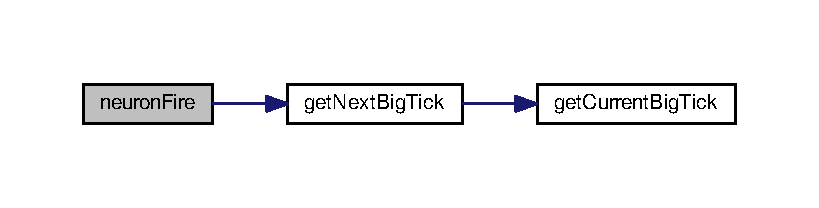
\includegraphics[width=350pt]{neuron_8h_a683379b633b55058dd5b8b67929c165c_cgraph}
\end{center}
\end{figure}


\hypertarget{neuron_8h_aabaff47eadb1e61b34c19b6e982f6511}{}\index{neuron.\+h@{neuron.\+h}!neuron\+Post\+Integrate@{neuron\+Post\+Integrate}}
\index{neuron\+Post\+Integrate@{neuron\+Post\+Integrate}!neuron.\+h@{neuron.\+h}}
\subsubsection[{neuron\+Post\+Integrate}]{\setlength{\rightskip}{0pt plus 5cm}void neuron\+Post\+Integrate (
\begin{DoxyParamCaption}
\item[{{\bf neuron\+State} $\ast$}]{st, }
\item[{tw\+\_\+stime}]{time, }
\item[{tw\+\_\+lp $\ast$}]{lp, }
\item[{bool}]{will\+Fire}
\end{DoxyParamCaption}
)}\label{neuron_8h_aabaff47eadb1e61b34c19b6e982f6511}


Function that runs after integration \& firing, for reset function and threshold bounce calls. 


\begin{DoxyParams}{Parameters}
{\em st} & state \\
\hline
{\em time} & event time \\
\hline
{\em lp} & lp \\
\hline
{\em did\+Fire} & did the neuron fire during this big tick?\\
\hline
\end{DoxyParams}
\begin{DoxyRefDesc}{Todo}
\item[\hyperlink{todo__todo000007}{Todo}]There is potentially an issue here -\/ does the True\+North architecture draw a new pseudorandom number during the threshold, fire, reset functions, or does it resuse them? It looks like re-\/use, so that\textquotesingle{}s what I\textquotesingle{}m doing here. \end{DoxyRefDesc}


Definition at line \hyperlink{neuron_8c_source_l00214}{214} of file \hyperlink{neuron_8c_source}{neuron.\+c}.



References \hyperlink{assist_8h_source_l00023}{\+\_\+rand\+T}, \hyperlink{assist_8h_source_l00022}{\+\_\+thresh\+T}, \hyperlink{assist_8h_source_l00020}{\+\_\+volt\+T}, \hyperlink{neuron_8h_source_l00177}{neuron\+State\+::do\+Reset}, \hyperlink{neuron_8h_source_l00158}{neuron\+State\+::drawn\+Random\+Number}, \hyperlink{assist_8h_source_l00048}{D\+T}, \hyperlink{neuron_8h_source_l00153}{neuron\+State\+::membrane\+Pot}, \hyperlink{neuron_8h_source_l00156}{neuron\+State\+::negative\+Threshold}, \hyperlink{neuron_8h_source_l00182}{neuron\+State\+::neg\+Thres\+Reset}, \hyperlink{neuron_8h_source_l00180}{neuron\+State\+::reset\+Mode}, and \hyperlink{neuron_8h_source_l00160}{neuron\+State\+::reset\+Voltage}.



Referenced by \hyperlink{neuron_8c_source_l00103}{neuron\+Receive\+Message()}.


\begin{DoxyCode}
00214                                                                                   \{
00215     \textcolor{keywordflow}{if}(willFire)\{ \textcolor{comment}{// neuron will/did fire:}
00216         st->\hyperlink{structneuron_state_afcf9d931e4fda519c43b4efeab687463}{doReset}(st);
00217     \} \textcolor{keywordflow}{else} \textcolor{keywordflow}{if} (st->\hyperlink{structneuron_state_a0fdd8f44c4105a94e17c4c58a51db486}{membranePot} < -1 * (st->\hyperlink{structneuron_state_a678bcd9f031e290178cd5d2855e74279}{negativeThreshold} * st->
      \hyperlink{structneuron_state_a3ec480684e7a2cfc67a8ef7ac1bf57b9}{negThresReset} + (st->\hyperlink{structneuron_state_a678bcd9f031e290178cd5d2855e74279}{negativeThreshold} + st->
      \hyperlink{structneuron_state_a296a4f04813c4882d6acd8c9074abd35}{drawnRandomNumber})))\{
00218             \textcolor{comment}{//sanity variables for the formulaic reset/bounce instead of calling functions:}
00219         \hyperlink{assist_8h_a5537d30256d443ce07efd3d879a4a720}{\_threshT} B = st->\hyperlink{structneuron_state_a678bcd9f031e290178cd5d2855e74279}{negativeThreshold};
00220         \textcolor{keywordtype}{int} K = st->\hyperlink{structneuron_state_a3ec480684e7a2cfc67a8ef7ac1bf57b9}{negThresReset};
00221         \textcolor{keywordtype}{int} G = st->\hyperlink{structneuron_state_af67bb650aa3150a6a31e16a874d71f91}{resetMode};
00222         \hyperlink{assist_8h_a520ac495f188eb0bc5645cffa3c4328b}{\_randT} n = st->\hyperlink{structneuron_state_a296a4f04813c4882d6acd8c9074abd35}{drawnRandomNumber};
00223         \hyperlink{assist_8h_abe1fc1b8f9efd1187e564bcb8de7f815}{\_voltT} R = st->\hyperlink{structneuron_state_af69a2c108fe9e7154fa047ea5acc5d80}{resetVoltage};
00224         \hyperlink{assist_8h_abe1fc1b8f9efd1187e564bcb8de7f815}{\_voltT} V = st->\hyperlink{structneuron_state_a0fdd8f44c4105a94e17c4c58a51db486}{membranePot};
00225         st->\hyperlink{structneuron_state_a0fdd8f44c4105a94e17c4c58a51db486}{membranePot} = (-(B*K) + (-(\hyperlink{assist_8h_acfde2b62c9c4e0413f3066bbd65c428a}{DT}(G)) * R +
00226                                      \hyperlink{assist_8h_acfde2b62c9c4e0413f3066bbd65c428a}{DT}(G-1) * (V + (B + n)) +
00227                                      \hyperlink{assist_8h_acfde2b62c9c4e0413f3066bbd65c428a}{DT}(G-2) * V) * (1-K));
00228 
00229     \}
00230 
00231 \}
\end{DoxyCode}
\hypertarget{neuron_8h_aa6819d7492f0173f2234ba0b8b0bb674}{}\index{neuron.\+h@{neuron.\+h}!neuron\+Receive\+Message@{neuron\+Receive\+Message}}
\index{neuron\+Receive\+Message@{neuron\+Receive\+Message}!neuron.\+h@{neuron.\+h}}
\subsubsection[{neuron\+Receive\+Message}]{\setlength{\rightskip}{0pt plus 5cm}void neuron\+Receive\+Message (
\begin{DoxyParamCaption}
\item[{{\bf neuron\+State} $\ast$}]{st, }
\item[{tw\+\_\+stime}]{time, }
\item[{{\bf Msg\+\_\+\+Data} $\ast$}]{m, }
\item[{tw\+\_\+lp $\ast$}]{lp}
\end{DoxyParamCaption}
)}\label{neuron_8h_aa6819d7492f0173f2234ba0b8b0bb674}


handles incomming synapse messages. 

In this model, the neurons send messages to axons during \char`\"{}big tick\char`\"{} intervals. This is done through an event sent upon receipt of the first synapse message of the current big-\/tick.


\begin{DoxyParams}{Parameters}
{\em st} & current neuron state \\
\hline
{\em time} & time event was received \\
\hline
{\em m} & event message data \\
\hline
{\em lp} & lp.\\
\hline
\end{DoxyParams}
neruon\+Receive\+Message runs when an event is received by a neuron. The events are handled in the following fashion\+:
\begin{DoxyItemize}
\item If the event is a synapse, the neuron integrates the weight of the synapse into its membrane potential.
\begin{DoxyItemize}
\item The count of big-\/tick synapse messages recived is incremented.
\item If the count changes from zero to one, the function creates and queues a heartbeat event for the next big-\/tick.
\end{DoxyItemize}
\item If the event is a heartbeat, the neuron will leak, potentially fire, and reset.
\end{DoxyItemize}

Big-\/\+Tick events are sent at time $𝒯_{bigTick} - ε$, so that the the event will arrive at the next bit-\/tick time. 

Definition at line \hyperlink{neuron_8c_source_l00103}{103} of file \hyperlink{neuron_8c_source}{neuron.\+c}.



References \hyperlink{neuron_8h_source_l00205}{neuron\+State\+::do\+Leak}, \hyperlink{neuron_8h_source_l00158}{neuron\+State\+::drawn\+Random\+Number}, \hyperlink{assist_8h_source_l00071}{Msg\+\_\+\+Data\+::event\+Type}, \hyperlink{neuron_8h_source_l00214}{neuron\+State\+::fire\+Count}, \hyperlink{neuron_8h_source_l00218}{neuron\+State\+::fired\+Last}, \hyperlink{neuron_8c_source_l00199}{integrate\+Synapse()}, \hyperlink{neuron_8h_source_l00161}{neuron\+State\+::last\+Active\+Time}, \hyperlink{neuron_8h_source_l00162}{neuron\+State\+::last\+Leak\+Time}, \hyperlink{assist_8h_source_l00073}{Msg\+\_\+\+Data\+::local\+I\+D}, \hyperlink{neuron_8h_source_l00153}{neuron\+State\+::membrane\+Pot}, \hyperlink{assist_8h_source_l00062}{N\+E\+U\+R\+O\+N\+\_\+\+H\+E\+A\+R\+T\+B\+E\+A\+T}, \hyperlink{neuron_8c_source_l00167}{neuron\+Fire()}, \hyperlink{neuron_8c_source_l00214}{neuron\+Post\+Integrate()}, \hyperlink{neuron_8c_source_l00161}{neuron\+Should\+Fire()}, \hyperlink{neuron_8h_source_l00215}{neuron\+State\+::rcvd\+Msg\+Count}, \hyperlink{neuron_8h_source_l00166}{neuron\+State\+::received\+Synapse\+Msgs}, \hyperlink{assist_8h_source_l00072}{Msg\+\_\+\+Data\+::rnd\+Call\+Count}, \hyperlink{neuron_8h_source_l00164}{neuron\+State\+::saved\+Last\+Active\+Time}, \hyperlink{neuron_8h_source_l00165}{neuron\+State\+::saved\+Last\+Leak\+Time}, \hyperlink{neuron_8h_source_l00154}{neuron\+State\+::saved\+Membrane\+Pot}, \hyperlink{neuron_8c_source_l00179}{send\+Heartbeat()}, \hyperlink{neuron_8h_source_l00216}{neuron\+State\+::\+S\+O\+P\+S\+Count}, \hyperlink{assist_8h_source_l00060}{S\+Y\+N\+A\+P\+S\+E\+\_\+\+O\+U\+T}, and \hyperlink{neuron_8h_source_l00157}{neuron\+State\+::threshold\+P\+R\+N\+Mask}.


\begin{DoxyCode}
00104           \{
00105     \textcolor{keywordtype}{bool} willFire = \textcolor{keyword}{false};
00106     st->\hyperlink{structneuron_state_a287eb8703dbfb177165d31c8840646b8}{firedLast} = \textcolor{keyword}{false};
00107         \textcolor{comment}{//save the previous state of the neuron:}
00108     st->\hyperlink{structneuron_state_a50734a9ba605a083a90814b63d039a03}{savedLastLeakTime} = st->\hyperlink{structneuron_state_a6f4e4d8fc1cf0257b486e01f628d2656}{lastLeakTime};
00109     st->\hyperlink{structneuron_state_a6922b3f3041346eb83cfc6352a22277b}{savedLastActiveTime} = st->\hyperlink{structneuron_state_a0658ad1f8b57a00589c6ea84f9a4ab13}{lastActiveTime};
00110     st->\hyperlink{structneuron_state_a5efe5de0478ea513ed5d90d89a49fcca}{savedMembranePot} = st->\hyperlink{structneuron_state_a0fdd8f44c4105a94e17c4c58a51db486}{membranePot};
00111         \textcolor{comment}{//random fn call state management.}
00112     \textcolor{keywordtype}{unsigned} \textcolor{keywordtype}{long} startCount = lp->rng->count;
00113 
00114     \textcolor{keywordflow}{switch} (m->\hyperlink{struct_msg___data_a015b6eb45982e1842ee8fc389a099ced}{eventType}) \{
00115   \textcolor{keywordflow}{case} \hyperlink{assist_8h_a7c1688de451e0dea1e11617bce3ec450a6ad6b93d8a818550e7246f6e0d143afb}{SYNAPSE\_OUT}:
00116             \hyperlink{neuron_8c_ae630bdf5dd3744870968f07a6971659c}{integrateSynapse}(m->\hyperlink{struct_msg___data_aefc820e92a74047ec7ed74c1c45f818f}{localID}, st, lp);
00117 
00118                 \textcolor{comment}{//next, we will check if a heartbeat message should be sent}
00119             \textcolor{keywordflow}{if}(st->\hyperlink{structneuron_state_af8935bcba177f2f3dfb9119c39ef7dc5}{receivedSynapseMsgs} == 0) \{
00120                 \hyperlink{neuron_8c_a766dff9e530486b055e97ebe392268b8}{sendHeartbeat}(st, lp, time);
00121             \}
00122             st->\hyperlink{structneuron_state_af8935bcba177f2f3dfb9119c39ef7dc5}{receivedSynapseMsgs} ++;
00123 
00124 
00125             \textcolor{keywordflow}{break};
00126 
00127         \textcolor{keywordflow}{case} \hyperlink{assist_8h_a7c1688de451e0dea1e11617bce3ec450a226690009a653238a52339561e6c466e}{NEURON\_HEARTBEAT}:
00128             st->\hyperlink{structneuron_state_af8935bcba177f2f3dfb9119c39ef7dc5}{receivedSynapseMsgs} = 0;
00129                 \textcolor{comment}{//set up drawn random number for the heartbeat.}
00130             \textcolor{keywordflow}{if}(st->\hyperlink{structneuron_state_aa501d6ee7cacd5435deec79c07637b08}{thresholdPRNMask} != 0)
00131                 st->\hyperlink{structneuron_state_a296a4f04813c4882d6acd8c9074abd35}{drawnRandomNumber} = tw\_rand\_integer(lp->rng, 0, st->
      \hyperlink{structneuron_state_aa501d6ee7cacd5435deec79c07637b08}{thresholdPRNMask});
00132 
00133                 \textcolor{comment}{//Currently operates - leak->fire->(reset)}
00134             st->\hyperlink{structneuron_state_aa430f424f34dc59dc27736e27ec61320}{doLeak}(st, time);
00135             willFire = \hyperlink{neuron_8c_a3520b013e0c2f711b9f5c16e19306be6}{neuronShouldFire}(st,lp);
00136             \textcolor{keywordflow}{if}(willFire)\{
00137                 \hyperlink{neuron_8c_a683379b633b55058dd5b8b67929c165c}{neuronFire}(st, time, lp);
00138                 st->\hyperlink{structneuron_state_afe8825076c4cf3863c677307fec63c61}{fireCount} ++;
00139             \}
00140 
00141             \hyperlink{neuron_8c_aabaff47eadb1e61b34c19b6e982f6511}{neuronPostIntegrate}(st, time, lp, willFire);
00142             \textcolor{comment}{//stats collection}
00143             st->\hyperlink{structneuron_state_a71fbb9a79e8048b473b6e09d29a64bbe}{SOPSCount} ++;
00144             st->\hyperlink{structneuron_state_a0658ad1f8b57a00589c6ea84f9a4ab13}{lastActiveTime} = tw\_now(lp);
00145             \textcolor{keywordflow}{break};
00146 
00147   \textcolor{keywordflow}{default}:
00148                 \textcolor{comment}{//Error condition - non-valid input.}
00149             \textcolor{keywordflow}{break};
00150     \}
00151 
00152         \textcolor{comment}{//store the random calls in the message:}
00153     m->\hyperlink{struct_msg___data_a2e49a6bcc6c45ade722f746b1ea707f2}{rndCallCount} = lp->rng->count - startCount;
00154 
00155     st->\hyperlink{structneuron_state_ab8f63a1dfdb2992657530ff8a63fdc01}{rcvdMsgCount} ++;
00156 
00157 
00158 
00159 \}
\end{DoxyCode}


Here is the call graph for this function\+:\nopagebreak
\begin{figure}[H]
\begin{center}
\leavevmode
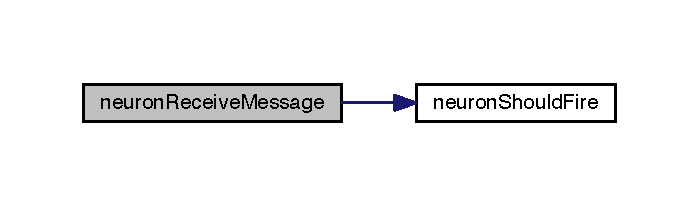
\includegraphics[width=350pt]{neuron_8h_aa6819d7492f0173f2234ba0b8b0bb674_cgraph}
\end{center}
\end{figure}


\hypertarget{neuron_8h_a01dcc8e3f0132786bd59ecb847013284}{}\index{neuron.\+h@{neuron.\+h}!neuron\+Reverse\+Final@{neuron\+Reverse\+Final}}
\index{neuron\+Reverse\+Final@{neuron\+Reverse\+Final}!neuron.\+h@{neuron.\+h}}
\subsubsection[{neuron\+Reverse\+Final}]{\setlength{\rightskip}{0pt plus 5cm}void neuron\+Reverse\+Final (
\begin{DoxyParamCaption}
\item[{{\bf neuron\+State} $\ast$}]{s, }
\item[{tw\+\_\+bf $\ast$}]{C\+V, }
\item[{{\bf Msg\+\_\+\+Data} $\ast$}]{m, }
\item[{tw\+\_\+lp $\ast$}]{lp}
\end{DoxyParamCaption}
)}\label{neuron_8h_a01dcc8e3f0132786bd59ecb847013284}


neuron\+Reverse\+Final final neuron reversal function. 

Used to roll back any calls made by the neuron. Decrements received\+Synapse\+Msgs Reset funs have already been run at this point \begin{DoxySeeAlso}{See also}
\hyperlink{neuron_8h_abf61b10b4b6116161a9e5c9d7ac54be1}{reverse\+Leak\+Del()} and 

\hyperlink{neuron_8h_aa939c0acc5b3367975f2f0cb7bc36d17}{reverse\+Reset\+Del()} 
\end{DoxySeeAlso}

\begin{DoxyParams}{Parameters}
{\em s} & the neuron state \\
\hline
{\em C\+V} & transported bitfield \\
\hline
{\em m} & the rollback message \\
\hline
{\em lp} & the lp \\
\hline
\end{DoxyParams}
\hypertarget{neuron_8h_a3520b013e0c2f711b9f5c16e19306be6}{}\index{neuron.\+h@{neuron.\+h}!neuron\+Should\+Fire@{neuron\+Should\+Fire}}
\index{neuron\+Should\+Fire@{neuron\+Should\+Fire}!neuron.\+h@{neuron.\+h}}
\subsubsection[{neuron\+Should\+Fire}]{\setlength{\rightskip}{0pt plus 5cm}bool neuron\+Should\+Fire (
\begin{DoxyParamCaption}
\item[{{\bf neuron\+State} $\ast$}]{st, }
\item[{tw\+\_\+lp $\ast$}]{lp}
\end{DoxyParamCaption}
)}\label{neuron_8h_a3520b013e0c2f711b9f5c16e19306be6}


Checks to see if a neuron should fire. 

\begin{DoxyRefDesc}{Todo}
\item[\hyperlink{todo__todo000008}{Todo}]check to see if this is needed, since it looks like just a simple if statement is in order.\end{DoxyRefDesc}



\begin{DoxyParams}{Parameters}
{\em st} & neuron state\\
\hline
\end{DoxyParams}
\begin{DoxyReturn}{Returns}
true if the neuron is ready to fire. 
\end{DoxyReturn}


Definition at line \hyperlink{neuron_8c_source_l00161}{161} of file \hyperlink{neuron_8c_source}{neuron.\+c}.



References \hyperlink{neuron_8h_source_l00158}{neuron\+State\+::drawn\+Random\+Number}, \hyperlink{neuron_8h_source_l00153}{neuron\+State\+::membrane\+Pot}, and \hyperlink{neuron_8h_source_l00155}{neuron\+State\+::threshold}.



Referenced by \hyperlink{neuron_8c_source_l00103}{neuron\+Receive\+Message()}.


\begin{DoxyCode}
00161                                                  \{
00162         \textcolor{comment}{//check negative threshold values:}
00163 
00164     \textcolor{keywordflow}{return} st->\hyperlink{structneuron_state_a0fdd8f44c4105a94e17c4c58a51db486}{membranePot} >= st->\hyperlink{structneuron_state_a132470c4c17828c209e3403ccf7ee680}{threshold} + st->
      \hyperlink{structneuron_state_a296a4f04813c4882d6acd8c9074abd35}{drawnRandomNumber};
00165 \}
\end{DoxyCode}
\hypertarget{neuron_8h_a8e52befc10f975c6be39cc93af573d7e}{}\index{neuron.\+h@{neuron.\+h}!no\+Leak@{no\+Leak}}
\index{no\+Leak@{no\+Leak}!neuron.\+h@{neuron.\+h}}
\subsubsection[{no\+Leak}]{\setlength{\rightskip}{0pt plus 5cm}void no\+Leak (
\begin{DoxyParamCaption}
\item[{void $\ast$}]{neuron, }
\item[{tw\+\_\+stime}]{now}
\end{DoxyParamCaption}
)}\label{neuron_8h_a8e52befc10f975c6be39cc93af573d7e}


no\+Leak -\/ A non leaking neuron function. 


\begin{DoxyParams}{Parameters}
{\em neuron} & The current neuron state. \\
\hline
{\em now} & The current simulation time. \\
\hline
\end{DoxyParams}


Definition at line \hyperlink{neuron_8c_source_l00016}{16} of file \hyperlink{neuron_8c_source}{neuron.\+c}.


\begin{DoxyCode}
00016                                         \{
00017   \textcolor{comment}{// do nothing!!}
00018 \}
\end{DoxyCode}
\hypertarget{neuron_8h_a2e78d7d2b70bf7349c3854b3727dcc25}{}\index{neuron.\+h@{neuron.\+h}!reset\+Linear@{reset\+Linear}}
\index{reset\+Linear@{reset\+Linear}!neuron.\+h@{neuron.\+h}}
\subsubsection[{reset\+Linear}]{\setlength{\rightskip}{0pt plus 5cm}void reset\+Linear (
\begin{DoxyParamCaption}
\item[{void $\ast$}]{neuron\+State}
\end{DoxyParamCaption}
)}\label{neuron_8h_a2e78d7d2b70bf7349c3854b3727dcc25}


Resets neuron voltage based on linear function. 


\begin{DoxyParams}{Parameters}
{\em \hyperlink{structneuron_state}{neuron\+State}} & \hyperlink{structneuron_state}{neuron\+State}\\
\hline
\end{DoxyParams}
Linear reset mode -\/ ignores $R$, and sets the membrane potential to the difference between the threshold and the potential. 

Definition at line \hyperlink{neuron_8c_source_l00066}{66} of file \hyperlink{neuron_8c_source}{neuron.\+c}.


\begin{DoxyCode}
00066                                     \{
00067     \textcolor{keyword}{struct }NeuronModel *s = (\textcolor{keyword}{struct }NeuronModel *)\hyperlink{structneuron_state}{neuronState};
00068     s->\hyperlink{structneuron_state_a0fdd8f44c4105a94e17c4c58a51db486}{membranePot} = s->membranePot - s->threshold;
00069 \}
\end{DoxyCode}
\hypertarget{neuron_8h_a6e11be912b4860cd1978b2d8c49b9703}{}\index{neuron.\+h@{neuron.\+h}!reset\+None@{reset\+None}}
\index{reset\+None@{reset\+None}!neuron.\+h@{neuron.\+h}}
\subsubsection[{reset\+None}]{\setlength{\rightskip}{0pt plus 5cm}void reset\+None (
\begin{DoxyParamCaption}
\item[{void $\ast$}]{neuron\+State}
\end{DoxyParamCaption}
)}\label{neuron_8h_a6e11be912b4860cd1978b2d8c49b9703}


No reset function -\/ does not reset membrane potential after firing. 


\begin{DoxyParams}{Parameters}
{\em \hyperlink{structneuron_state}{neuron\+State}} & current neuron state. \\
\hline
\end{DoxyParams}
\hypertarget{neuron_8h_a233aa7ebe6cbfb664fe366a05a8dac1f}{}\index{neuron.\+h@{neuron.\+h}!reset\+Normal@{reset\+Normal}}
\index{reset\+Normal@{reset\+Normal}!neuron.\+h@{neuron.\+h}}
\subsubsection[{reset\+Normal}]{\setlength{\rightskip}{0pt plus 5cm}void reset\+Normal (
\begin{DoxyParamCaption}
\item[{void $\ast$}]{neuron\+State}
\end{DoxyParamCaption}
)}\label{neuron_8h_a233aa7ebe6cbfb664fe366a05a8dac1f}


Resets neuron voltage to $R$ after firing. 

a normal reset mode function.


\begin{DoxyParams}{Parameters}
{\em \hyperlink{structneuron_state}{neuron\+State}} & current neuron state \\
\hline
\end{DoxyParams}


Definition at line \hyperlink{neuron_8c_source_l00056}{56} of file \hyperlink{neuron_8c_source}{neuron.\+c}.


\begin{DoxyCode}
00056                                     \{
00057     \textcolor{keyword}{struct }NeuronModel *s = (\textcolor{keyword}{struct }NeuronModel *)\hyperlink{structneuron_state}{neuronState};
00058     s->\hyperlink{structneuron_state_a0fdd8f44c4105a94e17c4c58a51db486}{membranePot} = s->resetVoltage; \textcolor{comment}{// set current voltage to \(\backslash\)f$R\(\backslash\)f$.}
00059 \}
\end{DoxyCode}
\hypertarget{neuron_8h_a09e54832158e2f6abe898437979aae00}{}\index{neuron.\+h@{neuron.\+h}!reverse\+Reset\+Linear@{reverse\+Reset\+Linear}}
\index{reverse\+Reset\+Linear@{reverse\+Reset\+Linear}!neuron.\+h@{neuron.\+h}}
\subsubsection[{reverse\+Reset\+Linear}]{\setlength{\rightskip}{0pt plus 5cm}void reverse\+Reset\+Linear (
\begin{DoxyParamCaption}
\item[{void $\ast$}]{neuron\+State}
\end{DoxyParamCaption}
)}\label{neuron_8h_a09e54832158e2f6abe898437979aae00}


Definition at line \hyperlink{neuron_8c_source_l00071}{71} of file \hyperlink{neuron_8c_source}{neuron.\+c}.



References \hyperlink{assist_8h_source_l00020}{\+\_\+volt\+T}.


\begin{DoxyCode}
00071                                           \{
00072     \textcolor{keyword}{struct }NeuronModel *s = (\textcolor{keyword}{struct }NeuronModel *)\hyperlink{structneuron_state}{neuronState};
00073     \hyperlink{assist_8h_abe1fc1b8f9efd1187e564bcb8de7f815}{\_voltT} resetParam = (\hyperlink{assist_8h_abe1fc1b8f9efd1187e564bcb8de7f815}{\_voltT}) &resetParam;
00074     s->membranePot = s->membranePot + resetParam;
00075 \}
\end{DoxyCode}
\hypertarget{neuron_8h_a50b2475c0a8d745eb8f144b72d7eabdf}{}\index{neuron.\+h@{neuron.\+h}!reverse\+Reset\+None@{reverse\+Reset\+None}}
\index{reverse\+Reset\+None@{reverse\+Reset\+None}!neuron.\+h@{neuron.\+h}}
\subsubsection[{reverse\+Reset\+None}]{\setlength{\rightskip}{0pt plus 5cm}void reverse\+Reset\+None (
\begin{DoxyParamCaption}
\item[{void $\ast$}]{neuron\+State}
\end{DoxyParamCaption}
)}\label{neuron_8h_a50b2475c0a8d745eb8f144b72d7eabdf}
\hypertarget{neuron_8h_ae53276ccdb759ba1ea09806cbf9fc940}{}\index{neuron.\+h@{neuron.\+h}!reverse\+Reset\+Zero@{reverse\+Reset\+Zero}}
\index{reverse\+Reset\+Zero@{reverse\+Reset\+Zero}!neuron.\+h@{neuron.\+h}}
\subsubsection[{reverse\+Reset\+Zero}]{\setlength{\rightskip}{0pt plus 5cm}void reverse\+Reset\+Zero (
\begin{DoxyParamCaption}
\item[{void $\ast$}]{neuron\+State}
\end{DoxyParamCaption}
)}\label{neuron_8h_ae53276ccdb759ba1ea09806cbf9fc940}
\begin{DoxyRefDesc}{Todo}
\item[\hyperlink{todo__todo000006}{Todo}]\+: Check that this is the proper way to handle reset zero function \end{DoxyRefDesc}


Definition at line \hyperlink{neuron_8c_source_l00079}{79} of file \hyperlink{neuron_8c_source}{neuron.\+c}.


\begin{DoxyCode}
00079                                         \{
00080 
00081 \}
\end{DoxyCode}
\hypertarget{neuron_8h_a26ced40d7ad7a0b448a136d8724fe18b}{}\index{neuron.\+h@{neuron.\+h}!rev\+Linear\+Leak@{rev\+Linear\+Leak}}
\index{rev\+Linear\+Leak@{rev\+Linear\+Leak}!neuron.\+h@{neuron.\+h}}
\subsubsection[{rev\+Linear\+Leak}]{\setlength{\rightskip}{0pt plus 5cm}void rev\+Linear\+Leak (
\begin{DoxyParamCaption}
\item[{void $\ast$}]{neuron, }
\item[{tw\+\_\+stime}]{now}
\end{DoxyParamCaption}
)}\label{neuron_8h_a26ced40d7ad7a0b448a136d8724fe18b}


Reverse leak function neurons that have a linear leak function assigned. 


\begin{DoxyParams}{Parameters}
{\em neuron} & current neuron state \\
\hline
{\em now} & tw\+\_\+stime representing current time of simulation. \\
\hline
\end{DoxyParams}


Definition at line \hyperlink{neuron_8c_source_l00037}{37} of file \hyperlink{neuron_8c_source}{neuron.\+c}.



References \hyperlink{neuron_8h_source_l00162}{neuron\+State\+::last\+Leak\+Time}.


\begin{DoxyCode}
00037                                               \{
00038     \hyperlink{structneuron_state}{neuronState} *s = (\hyperlink{structneuron_state}{neuronState} *)neuron;
00039     tw\_stime delta = s->\hyperlink{structneuron_state_a6f4e4d8fc1cf0257b486e01f628d2656}{lastLeakTime} - now;
00040 
00041         \textcolor{comment}{//s->membranePot += s->leakRate * delta;}
00042     s->\hyperlink{structneuron_state_a6f4e4d8fc1cf0257b486e01f628d2656}{lastLeakTime} = now;
00043 \}
\end{DoxyCode}
\hypertarget{neuron_8h_ac5bebec77c5216533ec5f6acd086532e}{}\index{neuron.\+h@{neuron.\+h}!rev\+No\+Leak@{rev\+No\+Leak}}
\index{rev\+No\+Leak@{rev\+No\+Leak}!neuron.\+h@{neuron.\+h}}
\subsubsection[{rev\+No\+Leak}]{\setlength{\rightskip}{0pt plus 5cm}void rev\+No\+Leak (
\begin{DoxyParamCaption}
\item[{void $\ast$}]{neuron, }
\item[{tw\+\_\+stime}]{now}
\end{DoxyParamCaption}
)}\label{neuron_8h_ac5bebec77c5216533ec5f6acd086532e}


Reverse leak function for use when neurons have no defined leak function. 


\begin{DoxyParams}{Parameters}
{\em neuron} & current neuron state \\
\hline
{\em now} & tw\+\_\+stime representing current time of simulation. \\
\hline
\end{DoxyParams}


Definition at line \hyperlink{neuron_8c_source_l00019}{19} of file \hyperlink{neuron_8c_source}{neuron.\+c}.


\begin{DoxyCode}
00019                                            \{
00020   \textcolor{comment}{// do nothing!!}
00021 \}
\end{DoxyCode}
\hypertarget{neuron_8h_a766dff9e530486b055e97ebe392268b8}{}\index{neuron.\+h@{neuron.\+h}!send\+Heartbeat@{send\+Heartbeat}}
\index{send\+Heartbeat@{send\+Heartbeat}!neuron.\+h@{neuron.\+h}}
\subsubsection[{send\+Heartbeat}]{\setlength{\rightskip}{0pt plus 5cm}void send\+Heartbeat (
\begin{DoxyParamCaption}
\item[{{\bf neuron\+State} $\ast$}]{st, }
\item[{tw\+\_\+lp $\ast$}]{lp, }
\item[{tw\+\_\+stime}]{time}
\end{DoxyParamCaption}
)}\label{neuron_8h_a766dff9e530486b055e97ebe392268b8}


Function that sends a heartbeat message to this neuron. 


\begin{DoxyParams}{Parameters}
{\em lp} & $<$\#lp description\#$>$ \\
\hline
{\em time} & $<$\#time description\#$>$ \\
\hline
\end{DoxyParams}


Definition at line \hyperlink{neuron_8c_source_l00179}{179} of file \hyperlink{neuron_8c_source}{neuron.\+c}.



References \hyperlink{assist_8h_source_l00071}{Msg\+\_\+\+Data\+::event\+Type}, \hyperlink{assist_8c_source_l00041}{get\+Next\+Big\+Tick()}, \hyperlink{assist_8h_source_l00073}{Msg\+\_\+\+Data\+::local\+I\+D}, \hyperlink{neuron_8h_source_l00149}{neuron\+State\+::my\+Local\+I\+D}, and \hyperlink{assist_8h_source_l00062}{N\+E\+U\+R\+O\+N\+\_\+\+H\+E\+A\+R\+T\+B\+E\+A\+T}.



Referenced by \hyperlink{neuron_8c_source_l00103}{neuron\+Receive\+Message()}.


\begin{DoxyCode}
00179                                                              \{
00180         \textcolor{comment}{//heartbeat message gen:}
00181     tw\_stime nextHeartbeat = \hyperlink{assist_8c_aa961bc9b414f1429b123fc8212c989fd}{getNextBigTick}(time);
00182     tw\_event *newEvent = tw\_event\_new(lp->gid, nextHeartbeat, lp);
00183     \hyperlink{struct_msg___data}{Msg\_Data} *data = (\hyperlink{struct_msg___data}{Msg\_Data} *) tw\_event\_data(newEvent);
00184     data->\hyperlink{struct_msg___data_a015b6eb45982e1842ee8fc389a099ced}{eventType} = \hyperlink{assist_8h_a7c1688de451e0dea1e11617bce3ec450a226690009a653238a52339561e6c466e}{NEURON\_HEARTBEAT};
00185     data->\hyperlink{struct_msg___data_aefc820e92a74047ec7ed74c1c45f818f}{localID} = st->\hyperlink{structneuron_state_ac24762c24aede292a2ce5df78114881c}{myLocalID};
00186     tw\_event\_send(newEvent);
00187 
00188 
00189 \}
\end{DoxyCode}


Here is the call graph for this function\+:\nopagebreak
\begin{figure}[H]
\begin{center}
\leavevmode
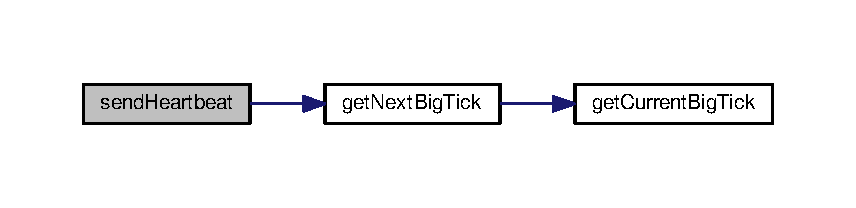
\includegraphics[width=350pt]{neuron_8h_a766dff9e530486b055e97ebe392268b8_cgraph}
\end{center}
\end{figure}


\hypertarget{neuron_8h_afee2e0acc66d8d10aee8d52c8d245c82}{}\index{neuron.\+h@{neuron.\+h}!stochastic\+Integrate@{stochastic\+Integrate}}
\index{stochastic\+Integrate@{stochastic\+Integrate}!neuron.\+h@{neuron.\+h}}
\subsubsection[{stochastic\+Integrate}]{\setlength{\rightskip}{0pt plus 5cm}void stochastic\+Integrate (
\begin{DoxyParamCaption}
\item[{{\bf \+\_\+weight\+T}}]{weight, }
\item[{{\bf neuron\+State} $\ast$}]{st, }
\item[{tw\+\_\+lp $\ast$}]{lp}
\end{DoxyParamCaption}
)}\label{neuron_8h_afee2e0acc66d8d10aee8d52c8d245c82}


Neuron stochastic integration function -\/ for use with stochastic leaks and synapse messages. 


\begin{DoxyParams}{Parameters}
{\em weight} & weight of selected leak or synapse \\
\hline
{\em st} & the neuron state \\
\hline
{\em lp} & lp for range functions. \\
\hline
\end{DoxyParams}


Definition at line \hyperlink{neuron_8c_source_l00191}{191} of file \hyperlink{neuron_8c_source}{neuron.\+c}.



References \hyperlink{assist_8h_source_l00052}{B\+I\+N\+C\+O\+M\+P}, \hyperlink{neuron_8h_source_l00158}{neuron\+State\+::drawn\+Random\+Number}, \hyperlink{neuron_8h_source_l00153}{neuron\+State\+::membrane\+Pot}, and \hyperlink{assist_8h_source_l00050}{S\+G\+N}.



Referenced by \hyperlink{neuron_8c_source_l00199}{integrate\+Synapse()}.


\begin{DoxyCode}
00191                                                                      \{
00192     \textcolor{keywordtype}{long} drawnRandom = st->\hyperlink{structneuron_state_a296a4f04813c4882d6acd8c9074abd35}{drawnRandomNumber};
00193     \textcolor{keywordflow}{if} (\hyperlink{assist_8h_abbf94867faa4abd8c53c87576efd05f3}{BINCOMP}(weight, drawnRandom))\{
00194         st->\hyperlink{structneuron_state_a0fdd8f44c4105a94e17c4c58a51db486}{membranePot} += \hyperlink{assist_8h_a95ed41486ca0ed53262e4b8934d4afac}{SGN}(weight);
00195     \}
00196 \}
\end{DoxyCode}

\hypertarget{neuron_8h_source}{}\section{neuron.\+h}
\label{neuron_8h_source}\index{/home/mplagge/development/tnt\+\_\+benchmark/models/neuron.\+h@{/home/mplagge/development/tnt\+\_\+benchmark/models/neuron.\+h}}

\begin{DoxyCode}
00001 \textcolor{comment}{//}
00002 \textcolor{comment}{//  neuron.h}
00003 \textcolor{comment}{//  ROSS\_TOP}
00004 \textcolor{comment}{//}
00005 \textcolor{comment}{//  Created by Mark Plagge on 6/18/15.}
00006 \textcolor{comment}{//}
00007 \textcolor{comment}{//}
00008 
00009 \textcolor{preprocessor}{#ifndef \_\_ROSS\_TOP\_\_neuron\_\_}
00010 \textcolor{preprocessor}{#define \_\_ROSS\_TOP\_\_neuron\_\_}
00011 
00012 \textcolor{preprocessor}{#include <stdio.h>}
00013 \textcolor{preprocessor}{#include "../assist.h"}
00014 \textcolor{preprocessor}{#include "../mapping.h"}
00015 \textcolor{preprocessor}{#include "ross.h"}
00016 \textcolor{preprocessor}{#include <stdbool.h>}
00017 
\hypertarget{neuron_8h_source_l00023}{}\hyperlink{neuron_8h_a48885ea6be5b55a2e24de9f97552d4ee}{00023}     \textcolor{keyword}{typedef} \textcolor{keyword}{enum} NeuronFireMode \{
\hypertarget{neuron_8h_source_l00024}{}\hyperlink{neuron_8h_a48885ea6be5b55a2e24de9f97552d4eea520c6b216334b8c2d914cf9fab8cd460}{00024}   \hyperlink{neuron_8h_a48885ea6be5b55a2e24de9f97552d4eea520c6b216334b8c2d914cf9fab8cd460}{NFM} = 0  \textcolor{comment}{// normal fire mode (if voltage > threshold, fire);}
00025     \} \hyperlink{neuron_8h_a48885ea6be5b55a2e24de9f97552d4ee}{neuronFireMode};
00026 
\hypertarget{neuron_8h_source_l00033}{}\hyperlink{neuron_8h_a7362d32c8d9b6dc323f5d1b05af9855b}{00033} \textcolor{keyword}{typedef} void (*\hyperlink{structleak_fun_del}{leakFunDel})(\textcolor{keywordtype}{void} *\hyperlink{structneuron_state}{neuronState}, tw\_stime now);
00034 
00041 \textcolor{keywordtype}{void} \hyperlink{neuron_8h_a8e52befc10f975c6be39cc93af573d7e}{noLeak}(\textcolor{keywordtype}{void} *neuron, tw\_stime now);
00048 \textcolor{keywordtype}{void} \hyperlink{neuron_8h_a64dc379b459a2b07b40bce35381210e8}{linearLeak}(\textcolor{keywordtype}{void} *neuron, tw\_stime now);
00049 
00050 \textcolor{keywordtype}{void} \hyperlink{neuron_8h_a5a4f7abf694fe6ff2aa68ebd5584bc4b}{monotonicUpLeak}(\textcolor{keywordtype}{void} *neuron, tw\_stime now);
00051 \textcolor{keywordtype}{void} \hyperlink{neuron_8h_a8c023bc2fc6d628a105b460226b106f9}{monotonicDownLeak}(\textcolor{keywordtype}{void} *neuron, tw\_stime now);
00052 
00053 \textcolor{keywordtype}{void} \hyperlink{neuron_8h_a5477909af0c953cabd578adf0695e5e5}{divergentLeak}(\textcolor{keywordtype}{void} *neuron, tw\_stime now);
00054 \textcolor{keywordtype}{void} \hyperlink{neuron_8h_ad5df8be6cabf9a00abf073cee3be0362}{convergentLeak}(\textcolor{keywordtype}{void} *neuron, tw\_stime now);
00055 
\hypertarget{neuron_8h_source_l00059}{}\hyperlink{neuron_8h_abf61b10b4b6116161a9e5c9d7ac54be1}{00059} \textcolor{keyword}{typedef} void (*\hyperlink{structreverse_leak_del}{reverseLeakDel})(\textcolor{keywordtype}{void} *neuron, tw\_stime now);
00060 
00067 \textcolor{keywordtype}{void} \hyperlink{neuron_8h_ac5bebec77c5216533ec5f6acd086532e}{revNoLeak}(\textcolor{keywordtype}{void} *neuron, tw\_stime now);
00068 
00075 \textcolor{keywordtype}{void} \hyperlink{neuron_8h_a26ced40d7ad7a0b448a136d8724fe18b}{revLinearLeak}(\textcolor{keywordtype}{void} *neuron, tw\_stime now);
00076 
\hypertarget{neuron_8h_source_l00080}{}\hyperlink{unionreset_rate}{00080} \textcolor{keyword}{typedef} \textcolor{keyword}{union }ResetRate \{
\hypertarget{neuron_8h_source_l00081}{}\hyperlink{unionreset_rate_a4bf8a23e4a9874ff73208c681eae1ced}{00081}     \textcolor{keywordtype}{int} \hyperlink{unionreset_rate_a4bf8a23e4a9874ff73208c681eae1ced}{linearRate};
\hypertarget{neuron_8h_source_l00082}{}\hyperlink{unionreset_rate_a54aaba14ce85fd9c5d7b385d98727e36}{00082}     \textcolor{keywordtype}{float} \hyperlink{unionreset_rate_a54aaba14ce85fd9c5d7b385d98727e36}{nonLinearRate};
\hypertarget{neuron_8h_source_l00083}{}\hyperlink{unionreset_rate_a5a9af6c017d8b70e4db9283f2f7e726b}{00083}     \hyperlink{assist_8h_abe1fc1b8f9efd1187e564bcb8de7f815}{\_voltT} \hyperlink{unionreset_rate_a5a9af6c017d8b70e4db9283f2f7e726b}{voltRate};
00084 \} \hyperlink{unionreset_rate}{resetRate};
00085 
\hypertarget{neuron_8h_source_l00094}{}\hyperlink{neuron_8h_ae7e5990745cd949246894bfb633ca4a2}{00094} \textcolor{keyword}{typedef} void (*\hyperlink{neuron_8h_ae7e5990745cd949246894bfb633ca4a2}{resetFunDel})(\textcolor{keywordtype}{void} *\hyperlink{structneuron_state}{neuronState});
00103 \textcolor{keywordtype}{void} \hyperlink{neuron_8h_a233aa7ebe6cbfb664fe366a05a8dac1f}{resetNormal}(\textcolor{keywordtype}{void} *\hyperlink{structneuron_state}{neuronState});
00104 
00110 \textcolor{keywordtype}{void} \hyperlink{neuron_8h_a2e78d7d2b70bf7349c3854b3727dcc25}{resetLinear}(\textcolor{keywordtype}{void} *\hyperlink{structneuron_state}{neuronState});
00116 \textcolor{keywordtype}{void} \hyperlink{neuron_8h_a6e11be912b4860cd1978b2d8c49b9703}{resetNone}(\textcolor{keywordtype}{void} *\hyperlink{structneuron_state}{neuronState});
00117 
00118 
00119 
\hypertarget{neuron_8h_source_l00125}{}\hyperlink{neuron_8h_aa939c0acc5b3367975f2f0cb7bc36d17}{00125} \textcolor{keyword}{typedef} void (*\hyperlink{neuron_8h_aa939c0acc5b3367975f2f0cb7bc36d17}{reverseResetDel})(\textcolor{keywordtype}{void} *\hyperlink{structneuron_state}{neuronState});
00126 
00127 \textcolor{keywordtype}{void} \hyperlink{neuron_8h_a09e54832158e2f6abe898437979aae00}{reverseResetLinear}(\textcolor{keywordtype}{void} *\hyperlink{structneuron_state}{neuronState});
00128 
00129 \textcolor{keywordtype}{void} \hyperlink{neuron_8h_ae53276ccdb759ba1ea09806cbf9fc940}{reverseResetZero}(\textcolor{keywordtype}{void} *\hyperlink{structneuron_state}{neuronState});
00130 
00131 \textcolor{keywordtype}{void} \hyperlink{neuron_8h_a50b2475c0a8d745eb8f144b72d7eabdf}{reverseResetNone}(\textcolor{keywordtype}{void} *\hyperlink{structneuron_state}{neuronState});
00132 
00133 
00134 
\hypertarget{neuron_8h_source_l00144}{}\hyperlink{structneuron_state}{00144} \textcolor{keyword}{typedef} \textcolor{keyword}{struct }NeuronModel \{
00147         \textcolor{comment}{//IDs and Lookup info}
\hypertarget{neuron_8h_source_l00148}{}\hyperlink{structneuron_state_a76ef99e5766b6e36c3f41a2920e8c56c}{00148}     \hyperlink{assist_8h_a3f7a6e6a1210b6d9d7a42177dcb9634b}{\_idT} \hyperlink{structneuron_state_a76ef99e5766b6e36c3f41a2920e8c56c}{myCoreID}; 
\hypertarget{neuron_8h_source_l00149}{}\hyperlink{structneuron_state_ac24762c24aede292a2ce5df78114881c}{00149}     \hyperlink{assist_8h_a3f7a6e6a1210b6d9d7a42177dcb9634b}{\_idT} \hyperlink{structneuron_state_ac24762c24aede292a2ce5df78114881c}{myLocalID}; 
00150 
00152         \textcolor{comment}{//Proper state information}
\hypertarget{neuron_8h_source_l00153}{}\hyperlink{structneuron_state_a0fdd8f44c4105a94e17c4c58a51db486}{00153}     \hyperlink{assist_8h_abe1fc1b8f9efd1187e564bcb8de7f815}{\_voltT} \hyperlink{structneuron_state_a0fdd8f44c4105a94e17c4c58a51db486}{membranePot}; 
\hypertarget{neuron_8h_source_l00154}{}\hyperlink{structneuron_state_a5efe5de0478ea513ed5d90d89a49fcca}{00154}     \hyperlink{assist_8h_abe1fc1b8f9efd1187e564bcb8de7f815}{\_voltT} \hyperlink{structneuron_state_a5efe5de0478ea513ed5d90d89a49fcca}{savedMembranePot}; 
\hypertarget{neuron_8h_source_l00155}{}\hyperlink{structneuron_state_a132470c4c17828c209e3403ccf7ee680}{00155}     \hyperlink{assist_8h_a5537d30256d443ce07efd3d879a4a720}{\_threshT} \hyperlink{structneuron_state_a132470c4c17828c209e3403ccf7ee680}{threshold}; 
\hypertarget{neuron_8h_source_l00156}{}\hyperlink{structneuron_state_a678bcd9f031e290178cd5d2855e74279}{00156}     \hyperlink{assist_8h_a5537d30256d443ce07efd3d879a4a720}{\_threshT} \hyperlink{structneuron_state_a678bcd9f031e290178cd5d2855e74279}{negativeThreshold}; 
\hypertarget{neuron_8h_source_l00157}{}\hyperlink{structneuron_state_aa501d6ee7cacd5435deec79c07637b08}{00157}     \hyperlink{assist_8h_a5537d30256d443ce07efd3d879a4a720}{\_threshT} \hyperlink{structneuron_state_aa501d6ee7cacd5435deec79c07637b08}{thresholdPRNMask}; 
\hypertarget{neuron_8h_source_l00158}{}\hyperlink{structneuron_state_a296a4f04813c4882d6acd8c9074abd35}{00158}     \hyperlink{assist_8h_a520ac495f188eb0bc5645cffa3c4328b}{\_randT} \hyperlink{structneuron_state_a296a4f04813c4882d6acd8c9074abd35}{drawnRandomNumber}; 
00159 
\hypertarget{neuron_8h_source_l00160}{}\hyperlink{structneuron_state_af69a2c108fe9e7154fa047ea5acc5d80}{00160}     \hyperlink{assist_8h_abe1fc1b8f9efd1187e564bcb8de7f815}{\_voltT} \hyperlink{structneuron_state_af69a2c108fe9e7154fa047ea5acc5d80}{resetVoltage}; 
\hypertarget{neuron_8h_source_l00161}{}\hyperlink{structneuron_state_a0658ad1f8b57a00589c6ea84f9a4ab13}{00161}     tw\_stime \hyperlink{structneuron_state_a0658ad1f8b57a00589c6ea84f9a4ab13}{lastActiveTime}; 
\hypertarget{neuron_8h_source_l00162}{}\hyperlink{structneuron_state_a6f4e4d8fc1cf0257b486e01f628d2656}{00162}     tw\_stime \hyperlink{structneuron_state_a6f4e4d8fc1cf0257b486e01f628d2656}{lastLeakTime};
\hypertarget{neuron_8h_source_l00164}{}\hyperlink{structneuron_state_a6922b3f3041346eb83cfc6352a22277b}{00164}     tw\_stime \hyperlink{structneuron_state_a6922b3f3041346eb83cfc6352a22277b}{savedLastActiveTime};
\hypertarget{neuron_8h_source_l00165}{}\hyperlink{structneuron_state_a50734a9ba605a083a90814b63d039a03}{00165}     tw\_stime \hyperlink{structneuron_state_a50734a9ba605a083a90814b63d039a03}{savedLastLeakTime}; 
\hypertarget{neuron_8h_source_l00166}{}\hyperlink{structneuron_state_af8935bcba177f2f3dfb9119c39ef7dc5}{00166}     uint\_fast16\_t \hyperlink{structneuron_state_af8935bcba177f2f3dfb9119c39ef7dc5}{receivedSynapseMsgs}; 
00173     \textcolor{comment}{/* neuron firing parameters */}
\hypertarget{neuron_8h_source_l00174}{}\hyperlink{structneuron_state_a55890f9e021064df30e9d18a9df98845}{00174}     \hyperlink{neuron_8h_a48885ea6be5b55a2e24de9f97552d4ee}{neuronFireMode} \hyperlink{structneuron_state_a55890f9e021064df30e9d18a9df98845}{fireMode}; 
00175 
\hypertarget{neuron_8h_source_l00177}{}\hyperlink{structneuron_state_afcf9d931e4fda519c43b4efeab687463}{00177}     \hyperlink{neuron_8h_ae7e5990745cd949246894bfb633ca4a2}{resetFunDel} \hyperlink{structneuron_state_afcf9d931e4fda519c43b4efeab687463}{doReset}; 
00178 
00179         \textcolor{comment}{//** as a test, this is the 𝛾 value - trying out mathematical reset style */}
\hypertarget{neuron_8h_source_l00180}{}\hyperlink{structneuron_state_af67bb650aa3150a6a31e16a874d71f91}{00180}     \textcolor{keywordtype}{short} \textcolor{keywordtype}{int} \hyperlink{structneuron_state_af67bb650aa3150a6a31e16a874d71f91}{resetMode};
00181 
\hypertarget{neuron_8h_source_l00182}{}\hyperlink{structneuron_state_a3ec480684e7a2cfc67a8ef7ac1bf57b9}{00182}     \textcolor{keywordtype}{bool} \hyperlink{structneuron_state_a3ec480684e7a2cfc67a8ef7ac1bf57b9}{negThresReset}; 
00183 
\hypertarget{neuron_8h_source_l00184}{}\hyperlink{structneuron_state_abf6970098695585c81e101b2a741b9a5}{00184}     \hyperlink{neuron_8h_aa939c0acc5b3367975f2f0cb7bc36d17}{reverseResetDel} \hyperlink{structneuron_state_abf6970098695585c81e101b2a741b9a5}{reverseReset}; 
00185 
00186         \textcolor{comment}{//Weight parameters}
\hypertarget{neuron_8h_source_l00187}{}\hyperlink{structneuron_state_aa71c0acf1edf08865e1f9729a2414efa}{00187}     \hyperlink{assist_8h_aa73c5ea0fe4ba938c96e6771b38dcb2a}{\_weightT} *\hyperlink{structneuron_state_aa71c0acf1edf08865e1f9729a2414efa}{synapticWeightProb}; 
\hypertarget{neuron_8h_source_l00192}{}\hyperlink{structneuron_state_a4568f103808a436a62d7c7c47dc90e9b}{00192}     \textcolor{keywordtype}{bool} *\hyperlink{structneuron_state_a4568f103808a436a62d7c7c47dc90e9b}{synapticWeightProbSelect}; 
00199         \textcolor{comment}{//Output locations:}
\hypertarget{neuron_8h_source_l00200}{}\hyperlink{structneuron_state_a62463fa4d33c39297aa5ce3a145d474f}{00200}     \hyperlink{assist_8h_a3f7a6e6a1210b6d9d7a42177dcb9634b}{\_idT} \hyperlink{structneuron_state_a62463fa4d33c39297aa5ce3a145d474f}{dendriteCore}; 
\hypertarget{neuron_8h_source_l00201}{}\hyperlink{structneuron_state_a73e5b16411af572181411b8fd8d5117d}{00201}     \hyperlink{assist_8h_a3f7a6e6a1210b6d9d7a42177dcb9634b}{\_idT} \hyperlink{structneuron_state_a73e5b16411af572181411b8fd8d5117d}{dendriteLocal}; 
\hypertarget{neuron_8h_source_l00202}{}\hyperlink{structneuron_state_a4199c14c5aabfd52f441e01623bdc84c}{00202}     tw\_lpid \hyperlink{structneuron_state_a4199c14c5aabfd52f441e01623bdc84c}{dendriteGlobalDest}; 
00203 
00204         \textcolor{comment}{//Leak functionality}
\hypertarget{neuron_8h_source_l00205}{}\hyperlink{structneuron_state_aa430f424f34dc59dc27736e27ec61320}{00205}     \hyperlink{structleak_fun_del}{leakFunDel} \hyperlink{structneuron_state_aa430f424f34dc59dc27736e27ec61320}{doLeak}; 
\hypertarget{neuron_8h_source_l00206}{}\hyperlink{structneuron_state_af4ded7f575b64ada6c0a6664f638307c}{00206}     \hyperlink{structreverse_leak_del}{reverseLeakDel} \hyperlink{structneuron_state_af4ded7f575b64ada6c0a6664f638307c}{doLeakReverse}; 
00207 
\hypertarget{neuron_8h_source_l00208}{}\hyperlink{structneuron_state_ac580cc92949834b3675de3aae267e8e7}{00208}     \hyperlink{assist_8h_aa73c5ea0fe4ba938c96e6771b38dcb2a}{\_weightT} \hyperlink{structneuron_state_ac580cc92949834b3675de3aae267e8e7}{leakRateProb}; 
\hypertarget{neuron_8h_source_l00209}{}\hyperlink{structneuron_state_a20889d9b55895bcc719d6aad2766b8f8}{00209}     \textcolor{keywordtype}{bool} \hyperlink{structneuron_state_a20889d9b55895bcc719d6aad2766b8f8}{leakWeightProbSelect}; 
00210 
\hypertarget{neuron_8h_source_l00211}{}\hyperlink{structneuron_state_a11691cf6bf906102089c842e78be55fe}{00211}     \textcolor{keywordtype}{bool} \hyperlink{structneuron_state_a11691cf6bf906102089c842e78be55fe}{leakReversalFlag}; 
00212 
00213         \textcolor{comment}{//Stats}
\hypertarget{neuron_8h_source_l00214}{}\hyperlink{structneuron_state_afe8825076c4cf3863c677307fec63c61}{00214}     \hyperlink{assist_8h_ad77e6fc5a9b03d46e7c97b7c4b92e89f}{\_statT} \hyperlink{structneuron_state_afe8825076c4cf3863c677307fec63c61}{fireCount}; 
\hypertarget{neuron_8h_source_l00215}{}\hyperlink{structneuron_state_ab8f63a1dfdb2992657530ff8a63fdc01}{00215}     \hyperlink{assist_8h_ad77e6fc5a9b03d46e7c97b7c4b92e89f}{\_statT} \hyperlink{structneuron_state_ab8f63a1dfdb2992657530ff8a63fdc01}{rcvdMsgCount}; 
\hypertarget{neuron_8h_source_l00216}{}\hyperlink{structneuron_state_a71fbb9a79e8048b473b6e09d29a64bbe}{00216}     \hyperlink{assist_8h_ad77e6fc5a9b03d46e7c97b7c4b92e89f}{\_statT} \hyperlink{structneuron_state_a71fbb9a79e8048b473b6e09d29a64bbe}{SOPSCount}; 
00217 
\hypertarget{neuron_8h_source_l00218}{}\hyperlink{structneuron_state_a287eb8703dbfb177165d31c8840646b8}{00218}     \textcolor{keywordtype}{bool} \hyperlink{structneuron_state_a287eb8703dbfb177165d31c8840646b8}{firedLast}; 
00219 
00220 \}\hyperlink{structneuron_state}{neuronState};
00221 
00222 \textcolor{comment}{/* ***Neuron functions */}
00232 \textcolor{keywordtype}{void} \hyperlink{neuron_8h_a01dcc8e3f0132786bd59ecb847013284}{neuronReverseFinal}(\hyperlink{structneuron_state}{neuronState} *s, tw\_bf *CV,
      \hyperlink{struct_msg___data}{Msg\_Data} *m,tw\_lp *lp);
00233 
00243 \textcolor{keywordtype}{void} \hyperlink{neuron_8h_aa6819d7492f0173f2234ba0b8b0bb674}{neuronReceiveMessage}(\hyperlink{structneuron_state}{neuronState} *st, tw\_stime time, 
      \hyperlink{struct_msg___data}{Msg\_Data} *m,
00244                           tw\_lp *lp);
00246 \textcolor{keywordtype}{void} \hyperlink{neuron_8h_a683379b633b55058dd5b8b67929c165c}{neuronFire}(\hyperlink{structneuron_state}{neuronState} *st, tw\_stime time, tw\_lp *lp);
00247 
00248 
00254 \textcolor{keywordtype}{void} \hyperlink{neuron_8h_ae630bdf5dd3744870968f07a6971659c}{integrateSynapse}(\hyperlink{assist_8h_a3f7a6e6a1210b6d9d7a42177dcb9634b}{\_idT} synapseID,\hyperlink{structneuron_state}{neuronState} *st, tw\_lp *lp);
00255 
00262 \textcolor{keywordtype}{void} \hyperlink{neuron_8h_a766dff9e530486b055e97ebe392268b8}{sendHeartbeat}(\hyperlink{structneuron_state}{neuronState} *st, tw\_lp *lp, tw\_stime time);
00263 
00271 \textcolor{keywordtype}{bool} \hyperlink{neuron_8h_a3520b013e0c2f711b9f5c16e19306be6}{neuronShouldFire}(\hyperlink{structneuron_state}{neuronState} *st, tw\_lp *lp);
00272 
00281 \textcolor{keywordtype}{void} \hyperlink{neuron_8h_aabaff47eadb1e61b34c19b6e982f6511}{neuronPostIntegrate}(\hyperlink{structneuron_state}{neuronState} *st, tw\_stime time, tw\_lp *lp, \textcolor{keywordtype}{bool} 
      willFire);
00289 \textcolor{keywordtype}{void} \hyperlink{neuron_8h_afee2e0acc66d8d10aee8d52c8d245c82}{stochasticIntegrate}(\hyperlink{assist_8h_aa73c5ea0fe4ba938c96e6771b38dcb2a}{\_weightT} weight, \hyperlink{structneuron_state}{neuronState} *st, tw\_lp *lp)
      ;
00290 
00291 
00292 \textcolor{keywordtype}{void} \hyperlink{neuron_8h_aaae24f12a4b2a537740f29d65eb3e51e}{neronReverseSate}(\hyperlink{structneuron_state}{neuronState} *s, tw\_bf *CV, 
      \hyperlink{struct_msg___data}{Msg\_Data} *M, tw\_lp *lp);
00293 
00294 \textcolor{preprocessor}{#endif }\textcolor{comment}{/* defined(\_\_ROSS\_TOP\_\_neuron\_\_) */}\textcolor{preprocessor}{}
\end{DoxyCode}

\hypertarget{synapse_8c}{}\section{/\+Users/\+Mark/\+Development/\+True\+North/tnt\+\_\+benchmark/models/synapse.c File Reference}
\label{synapse_8c}\index{/\+Users/\+Mark/\+Development/\+True\+North/tnt\+\_\+benchmark/models/synapse.\+c@{/\+Users/\+Mark/\+Development/\+True\+North/tnt\+\_\+benchmark/models/synapse.\+c}}
{\ttfamily \#include \char`\"{}synapse.\+h\char`\"{}}\\*
Include dependency graph for synapse.\+c\+:
\nopagebreak
\begin{figure}[H]
\begin{center}
\leavevmode
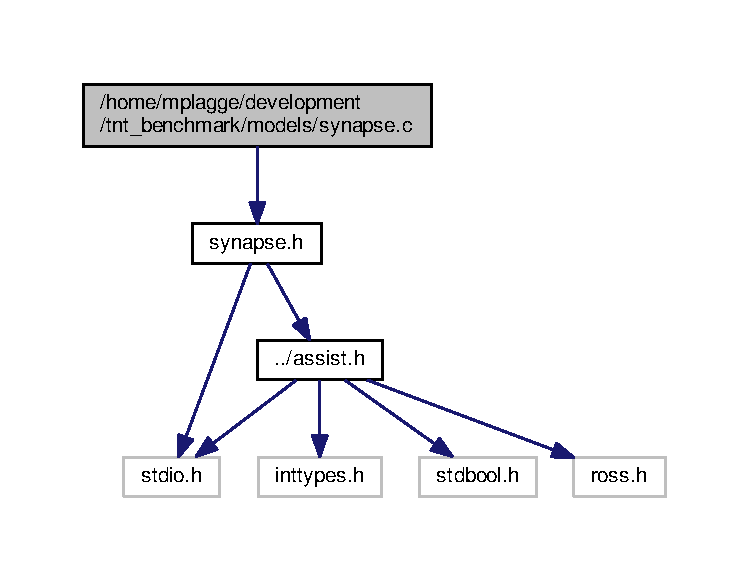
\includegraphics[width=344pt]{synapse_8c__incl}
\end{center}
\end{figure}

\hypertarget{synapse_8c_source}{}\section{synapse.\+c}
\label{synapse_8c_source}\index{/\+Users/\+Mark/\+Development/\+True\+North/tnt\+\_\+benchmark/models/synapse.\+c@{/\+Users/\+Mark/\+Development/\+True\+North/tnt\+\_\+benchmark/models/synapse.\+c}}

\begin{DoxyCode}
00001 \textcolor{comment}{//}
00002 \textcolor{comment}{//  synapse.c}
00003 \textcolor{comment}{//  ROSS\_TOP}
00004 \textcolor{comment}{//}
00005 \textcolor{comment}{//  Created by Mark Plagge on 6/18/15.}
00006 \textcolor{comment}{//}
00007 \textcolor{comment}{//}
00008 
00009 \textcolor{preprocessor}{#}\textcolor{preprocessor}{include} \hyperlink{synapse_8h}{"synapse.h"}
\end{DoxyCode}

\hypertarget{synapse_8h}{}\section{/\+Users/\+Mark/\+Development/\+True\+North/tnt\+\_\+benchmark/models/synapse.h File Reference}
\label{synapse_8h}\index{/\+Users/\+Mark/\+Development/\+True\+North/tnt\+\_\+benchmark/models/synapse.\+h@{/\+Users/\+Mark/\+Development/\+True\+North/tnt\+\_\+benchmark/models/synapse.\+h}}
{\ttfamily \#include $<$stdio.\+h$>$}\\*
{\ttfamily \#include \char`\"{}../assist.\+h\char`\"{}}\\*
{\ttfamily \#include \char`\"{}../input\+\_\+simulator.\+h\char`\"{}}\\*
Include dependency graph for synapse.\+h\+:
\nopagebreak
\begin{figure}[H]
\begin{center}
\leavevmode
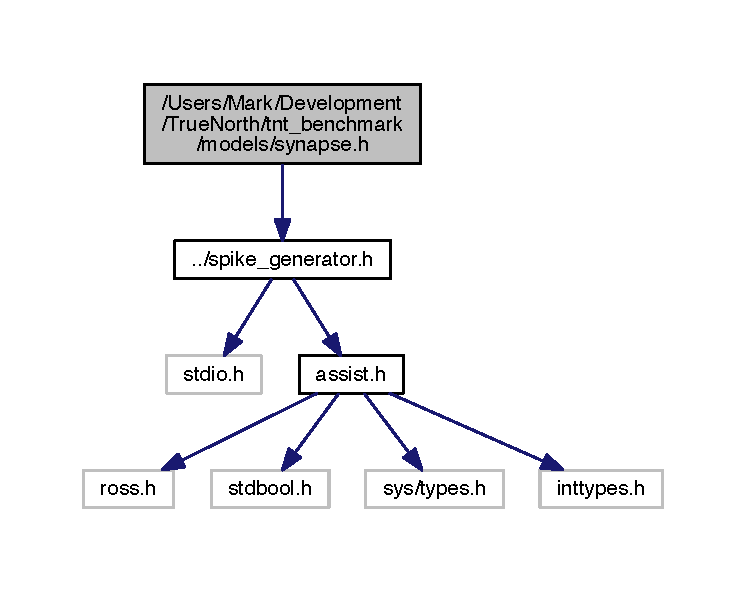
\includegraphics[width=344pt]{synapse_8h__incl}
\end{center}
\end{figure}
This graph shows which files directly or indirectly include this file\+:
\nopagebreak
\begin{figure}[H]
\begin{center}
\leavevmode
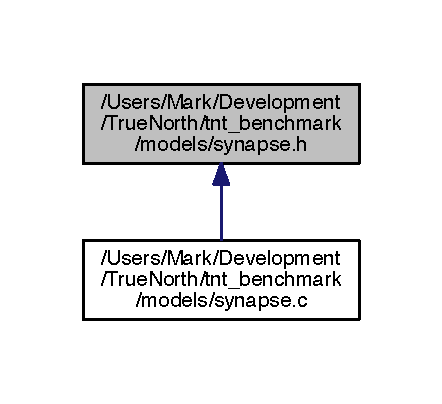
\includegraphics[width=212pt]{synapse_8h__dep__incl}
\end{center}
\end{figure}
\subsection*{Data Structures}
\begin{DoxyCompactItemize}
\item 
struct \hyperlink{structsynapse_state}{synapse\+State}
\begin{DoxyCompactList}\small\item\em Synapse state structure. \end{DoxyCompactList}\end{DoxyCompactItemize}

\hypertarget{synapse_8h_source}{}\section{synapse.\+h}
\label{synapse_8h_source}\index{/\+Users/\+Mark/\+Development/\+True\+North/tnt\+\_\+benchmark/models/synapse.\+h@{/\+Users/\+Mark/\+Development/\+True\+North/tnt\+\_\+benchmark/models/synapse.\+h}}

\begin{DoxyCode}
00001 \textcolor{comment}{//}
00002 \textcolor{comment}{//  synapse.h}
00003 \textcolor{comment}{//  ROSS\_TOP}
00004 \textcolor{comment}{//}
00005 \textcolor{comment}{//  Created by Mark Plagge on 6/18/15.}
00006 \textcolor{comment}{//}
00007 \textcolor{comment}{//}
00008 
00009 \textcolor{preprocessor}{#}\textcolor{preprocessor}{ifndef} \textcolor{preprocessor}{\_\_ROSS\_TOP\_\_synapse\_\_}
00010 \textcolor{preprocessor}{#}\textcolor{preprocessor}{define} \textcolor{preprocessor}{\_\_ROSS\_TOP\_\_synapse\_\_}
00011 
00012 \textcolor{preprocessor}{#}\textcolor{preprocessor}{include} \textcolor{preprocessor}{<}\textcolor{preprocessor}{stdio}\textcolor{preprocessor}{.}\textcolor{preprocessor}{h}\textcolor{preprocessor}{>}
00013 \textcolor{preprocessor}{#}\textcolor{preprocessor}{include} \textcolor{preprocessor}{"../assist.h"}
00014 \textcolor{preprocessor}{#}\textcolor{preprocessor}{include} \textcolor{preprocessor}{"../input\_simulator.h"}
00015 \textcolor{comment}{/**Synapse state structure. Synapses have a destination GID, calculated on creation from the current
       core and the mapping table. Each synapse talks to its connected neuron, sending messages to the neuron at a
       TS of ε, generated by the function in assist.h getNextEventTS. @see getNextEventTS(tw\_lp* lp). Synapses
       within the core, I.E., neuron nums < j-1, send a message at ε to the next synapse in the core. This simulates the
       "synaptic crossbar" found in the TrueNorth architecture.}
00016 \textcolor{comment}{ Synapses also have stats on sent neuron messages, and sent synapse messages. */}
00017 
\hypertarget{synapse_8h_source_l00018}{}\hyperlink{structsynapse_state}{00018} \textcolor{keyword}{typedef} \textcolor{keyword}{struct} \hyperlink{structsynapse_state}{SynapseState} \{
\hypertarget{synapse_8h_source_l00019}{}\hyperlink{structsynapse_state_a665999819b255f36d756f17b85bc9a03}{00019}     \hyperlink{structsynapse_state_a665999819b255f36d756f17b85bc9a03}{tw\_lpid} \hyperlink{structsynapse_state_a665999819b255f36d756f17b85bc9a03}{destSynapse};
\hypertarget{synapse_8h_source_l00020}{}\hyperlink{structsynapse_state_a0710dca002b4b3a3f7ae72633bef3691}{00020}     \hyperlink{structsynapse_state_a0710dca002b4b3a3f7ae72633bef3691}{tw\_lpid} \hyperlink{structsynapse_state_a0710dca002b4b3a3f7ae72633bef3691}{destNeuron};
\hypertarget{synapse_8h_source_l00021}{}\hyperlink{structsynapse_state_ab73db495221608d3eae73d51670d29f0}{00021}     \hyperlink{structsynapse_state_ab73db495221608d3eae73d51670d29f0}{id\_t} \hyperlink{structsynapse_state_ab73db495221608d3eae73d51670d29f0}{mySynapseNum};
\hypertarget{synapse_8h_source_l00022}{}\hyperlink{structsynapse_state_a9e389b0b50f9ec5e3f5b7b0f5383d6d5}{00022}     \hyperlink{assist_8h_ad77e6fc5a9b03d46e7c97b7c4b92e89f}{\_statT} \hyperlink{structsynapse_state_a9e389b0b50f9ec5e3f5b7b0f5383d6d5}{neuronMsgSent};
\hypertarget{synapse_8h_source_l00023}{}\hyperlink{structsynapse_state_a3fd766946f24d2fd6a2021ec24939284}{00023}     \hyperlink{assist_8h_ad77e6fc5a9b03d46e7c97b7c4b92e89f}{\_statT} \hyperlink{structsynapse_state_a3fd766946f24d2fd6a2021ec24939284}{synapseMsgSent};
00024 \}synapseState;
00025 
00026 
00027 \textcolor{preprocessor}{#}\textcolor{preprocessor}{endif} \textcolor{comment}{/* defined(\_\_ROSS\_TOP\_\_synapse\_\_) */}
\end{DoxyCode}

%--- End generated contents ---

% Index
\backmatter
\newpage
\phantomsection
\clearemptydoublepage
\addcontentsline{toc}{chapter}{Index}
\printindex

\end{document}
